\documentclass[11pt]{report}
\usepackage[margin=1in]{geometry}
\usepackage[T1,OT1]{fontenc}   % OT1 by default, T1 inside the chapters whose note uses it
\usepackage{amsmath,amssymb}
\usepackage{cancel}
\usepackage{xcolor}
\usepackage{booktabs}
\usepackage{array}
\usepackage{longtable}
\usepackage{graphicx}
\usepackage{placeins}
\usepackage{tikz}
\usetikzlibrary{arrows.meta,decorations.pathmorphing,decorations.markings,positioning,calc}
\usepackage[colorlinks=true,linkcolor=blue,citecolor=blue,urlcolor=blue]{hyperref}
\hypersetup{pdftitle={Inverse-bremsstrahlung heating of KrF laser gases: afterglow reheating as it stands},
  pdfauthor={Cooper K. Watson}}

%================================================================
%  Inverse-bremsstrahlung heating of KrF laser gases: a compendium.
%  Part I is written for the compendium (part1.tex). Part II is six
%  notes, one chapter each (chapters/<key>.tex with their tables and
%  figures in chapters/<key>/), assembled from the notes' sources with
%  every label, reference and citation key prefixed by the chapter's
%  key: env, qib, nl, lad, pd, ea. No hyperlinks inside table cells
%  (they crash macOS Preview): use \ref* and \nlcite there.
%================================================================

\setlength{\emergencystretch}{3em}
\setlength{\LTcapwidth}{\textwidth}
\setlength{\belowcaptionskip}{4pt}
\newcolumntype{L}[1]{>{\raggedright\arraybackslash}p{#1}}
\makeatletter
\newcommand{\tabinput}[1]{\@@input #1 }
\makeatother

% the notation of the six notes (one definition each; \avea is the
% electron-atom note's bold a, since the plasma derivation's \av is bold a_0)
\newcommand{\dd}{\mathrm d}
\newcommand{\kB}{k_B}
\newcommand{\ehat}{\hat{\mathbf e}}
\newcommand{\Ev}{\mathbf E}
\newcommand{\vv}{\mathbf v}
\newcommand{\jv}{\mathbf j}
\newcommand{\kv}{\mathbf k}
\newcommand{\pv}{\mathbf p}
\newcommand{\rv}{\mathbf r}
\newcommand{\Rv}{\mathbf R}
\newcommand{\Av}{\mathbf A}
\newcommand{\Qv}{\mathbf Q}
\newcommand{\av}{\mathbf a_0}
\newcommand{\avea}{\mathbf a}
\newcommand{\Vol}{\mathcal V}
\newcommand{\vosc}{\mathbf v_{\rm osc}}
\newcommand{\vos}{v_{\rm os}}
\newcommand{\Up}{U_{\rm p}}
\newcommand{\vt}{v_t}
\newcommand{\nuT}{\nu_T}
\newcommand{\nueff}{\nu_{\rm eff}}
\newcommand{\nuea}{\nu_{ea}}
\newcommand{\nuei}{\nu_{ei}}
\newcommand{\num}{\nu_m}
\newcommand{\Te}{T_e}
\newcommand{\fbest}{f_{\rm best}}
\newcommand{\lnL}{\ln\Lambda}
\newcommand{\sm}{\sigma_{\rm m}}
\newcommand{\Ebar}{\bar E}
\newcommand{\lambdabar}{{\mkern0.75mu\mathchar'26\mkern-9.75mu\lambda}}
\DeclareMathOperator{\Imag}{Im}
\DeclareMathOperator{\Real}{Re}
\DeclareMathOperator{\sgn}{sgn}
\DeclareMathOperator{\erf}{erf}

% chapters: the note's date under its title, its appendices as sections
% A, B, ... of the chapter, its abstract, and its bibliography as a section
\newcommand{\notedate}[1]{\noindent{\small\itshape The note of #1.}\par\medskip}
\makeatletter
\newcommand{\chapterappendix}{%
  \setcounter{section}{0}%
  \renewcommand{\thesection}{\thechapter.\Alph{section}}%
  \renewcommand{\theHsection}{\thechapter.app.\Alph{section}}}
\renewenvironment{thebibliography}[1]
  {\section*{References}%
   \addcontentsline{toc}{section}{References}%
   \list{\@biblabel{\@arabic\c@enumiv}}%
        {\settowidth\labelwidth{\@biblabel{#1}}%
         \leftmargin\labelwidth
         \advance\leftmargin\labelsep
         \@openbib@code
         \usecounter{enumiv}%
         \let\p@enumiv\@empty
         \renewcommand\theenumiv{\@arabic\c@enumiv}}%
   \sloppy
   \clubpenalty4000
   \@clubpenalty \clubpenalty
   \widowpenalty4000%
   \sfcode`\.\@m}
  {\def\@noitemerr
     {\@latex@warning{Empty `thebibliography' environment}}%
   \endlist}
\makeatother
\newenvironment{chapterabstract}{\begin{quote}\small\noindent\textbf{Abstract.}\ }{\end{quote}}
% a citation without a link, for table cells
\newcommand{\nlcite}[1]{\begin{NoHyper}\cite{#1}\end{NoHyper}}

\begin{document}
% the title page, the contents and the body each number their own pages,
% so that no two pages share a page anchor
\pagenumbering{alph}
\begin{titlepage}
\centering
\vspace*{2cm}
{\LARGE\bfseries Inverse-bremsstrahlung heating\\[4pt] of KrF laser gases\par}
\vspace{0.8cm}
{\large Afterglow reheating as it stands, and the six notes behind it\par}
\vspace{1.2cm}
{\large Cooper K.\ Watson\par}
\vspace{0.4cm}
{\large October 20, 2026\par}
\vspace{1.6cm}
\begin{minipage}{0.86\textwidth}
\small
\noindent This compendium collects six notes on the heating of the free electrons of KrF
laser gases by inverse bremsstrahlung, and asks of them one question: can an
electromagnetic wave that reheats the electrons of the afterglow, after the electron beam
has stopped, make the laser more efficient? Part~I answers it as the notes stand. The
heating half of the proposal is verified in silico. At the afterglow's
$10^{20}$~m$^{-3}$ a wave of 0.64 to 3.8~THz is absorbed through 10~cm of gas, where
microwaves heat a layer millimetres deep, the absorption coefficient is known to 1.6\,\%
in its kernel and to about 20\,\% in krypton's cross section at the afterglow's
0.63~eV, and $1.4\times10^{3}$ to $1.5\times10^{4}$~W\,cm$^{-2}$ holds the electrons, far
from the nonlinear regimes of Langdon and Silin. The efficiency half is open. A THz wave
would form 1.4 to 1.8 times the electron beam's KrF$^*$ per absorbed joule, but that
count leaves out the electron collisions of Kr$^*$ and KrF$^*$ on which the sign of the
gain rests, and no note follows the KrF$^*$ to laser energy or to the wall plug. The
nonlinearity of inverse bremsstrahlung and the laser's own field are invalidated as
levers. Part~I ends with the measurements and the calculation that would settle the
rest, and Part~II reproduces the six notes in full.
\end{minipage}
\end{titlepage}
\pagenumbering{roman}
\tableofcontents
\clearpage
\pagenumbering{arabic}

\part{Afterglow reheating: where the case stands}\label{p1:part:case}
%================================================================
%  Part I: afterglow reheating, where the case stands. Every number
%  is printed in the chapter cited next to it, or follows from such
%  numbers by the arithmetic shown. No hyperlinks inside table cells.
%================================================================

\chapter{The question and the verdict}
\label{p1:chap:verdict}

%================================================================
\section{The proposal}
\label{p1:sec:proposal}
%================================================================

{\noindent}(1) An electron beam pumps a KrF laser gas by making ion pairs and
excited atoms, and KrF$^*$ forms from them, much of it through the harpoon
reaction of excited krypton with F$_2$. When the beam stops, the electrons it
leaves behind cool and are lost to attachment and recombination. This is the
afterglow. Part~\ref{p1:part:notes} describes it in the neon-buffered fill of an
electron-beam-pumped laser, Ne/Kr/F$_2$ $=0.948/0.05/0.002$ at 2~atm, by
electrons at 0.63~eV and $10^{20}$~m$^{-3}$, against 1.5~eV and
$2.72\times10^{21}$~m$^{-3}$ with the beam on (Sec.~\ref{nl:sec:regime}). The
afterglow holds 27 times fewer electrons, and colder ones.

{\noindent}(2) Reheating sends an electromagnetic wave into the afterglow. The wave
heats the free electrons by inverse bremsstrahlung (IB), the hotter electrons
excite krypton again, and the excited krypton forms KrF$^*$ while F$_2$ lasts. The
question of this compendium is whether that can make the laser more efficient,
that is, raise the laser energy per unit of electrical energy.

{\noindent}(3) It can only if five links hold (Fig.~\ref{p1:fig:chain}):
\begin{itemize}
\item[L1] \emph{Coupling.} The wave enters the gas and is absorbed through the
  depth of the gain medium, rather than reflected or absorbed in a thin skin.
\item[L2] \emph{Absorption.} The absorption coefficient that decides L1 is known.
\item[L3] \emph{Heating.} An available intensity raises the electron temperature,
  in a regime that the kinetic equation of the electrons describes.
\item[L4] \emph{Partition.} The energy the electrons take from the wave forms
  KrF$^*$ at a useful efficiency.
\item[L5] \emph{Laser and wall plug.} Laser photons extract the KrF$^*$, and the
  source of the wave is efficient enough for the gain to pay.
\end{itemize}

{\noindent}(4) A link is called \emph{verified} here when the calculations of
Part~\ref{p1:part:notes} establish it, with their inputs tested against measurements
where the notes cite such tests. Nothing in Part~\ref{p1:part:notes} measures
reheating itself. A link or a lever is \emph{invalidated} when those calculations
rule it out, and \emph{open} when they do not settle it, in which case
Chapter~\ref{p1:chap:settle} names what would.

%================================================================
\section{The verdict}
\label{p1:sec:verdict}
%================================================================

{\noindent}(1) The heating half of the proposal stands, and the efficiency half is
open. Coupling, absorption and heating are verified in silico, with one constraint
that shapes the proposal: only the THz band heats the afterglow through
centimetres, while microwaves heat a layer millimetres deep. The partition favours
the field. At the afterglow's density a wave far above the collision frequency
forms KrF$^*$ at 1.4 to 1.8 times the electron beam's rate per absorbed joule, but
that count leaves out the electron collisions with Kr$^*$ and KrF$^*$ on which the
sign of the gain rests, and no note carries the KrF$^*$ to laser energy or to the
wall plug. Two levers are invalidated: the nonlinearity of IB, and the laser's own
field. Table~\ref{p1:tab:verdict} collects the verdict, and
Chapter~\ref{p1:chap:evidence} gives the evidence link by link.

\begin{figure}[t]
\centering
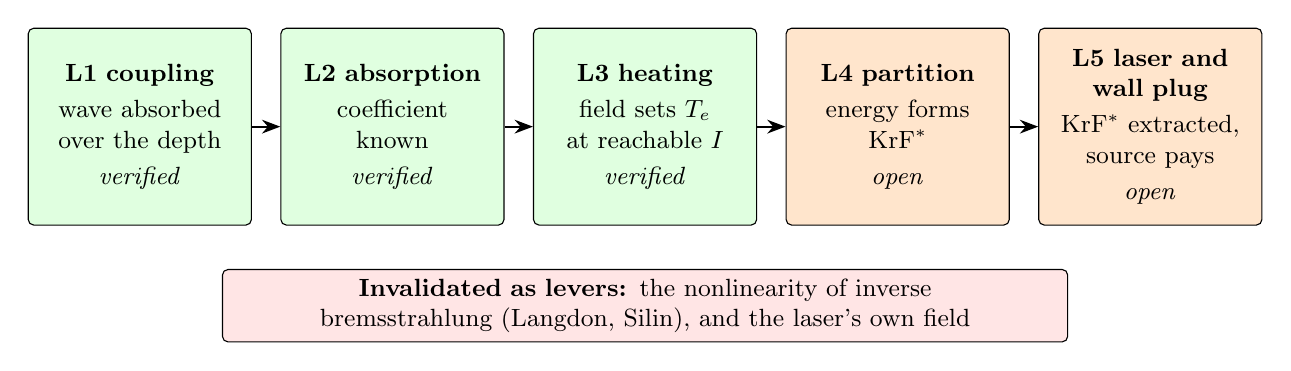
\begin{tikzpicture}[>=Stealth,
  link/.style={draw, rounded corners=2pt, align=center, text width=2.6cm,
    minimum height=2.5cm, font=\small},
  ver/.style={link, fill=green!12},
  opn/.style={link, fill=orange!20},
  inv/.style={draw, rounded corners=2pt, align=center, text width=10.5cm,
    font=\small, fill=red!10}]
\node[ver] (L1) {\textbf{L1 coupling}\\[2pt] wave absorbed\\ over the depth\\[2pt] \emph{verified}};
\node[ver, right=0.36cm of L1] (L2) {\textbf{L2 absorption}\\[2pt] coefficient\\ known\\[2pt] \emph{verified}};
\node[ver, right=0.36cm of L2] (L3) {\textbf{L3 heating}\\[2pt] field sets $T_e$\\ at reachable $I$\\[2pt] \emph{verified}};
\node[opn, right=0.36cm of L3] (L4) {\textbf{L4 partition}\\[2pt] energy forms\\ KrF$^*$\\[2pt] \emph{open}};
\node[opn, right=0.36cm of L4] (L5) {\textbf{L5 laser and}\\ \textbf{wall plug}\\[2pt] KrF$^*$ extracted,\\ source pays\\[2pt] \emph{open}};
\foreach \a/\b in {L1/L2,L2/L3,L3/L4,L4/L5} \draw[->,thick] (\a) -- (\b);
\node[inv, below=0.55cm of L3] (N) {\textbf{Invalidated as levers:} the nonlinearity of
  inverse bremsstrahlung (Langdon, Silin), and the laser's own field};
\end{tikzpicture}
\caption{The chain from the wave to the laser energy, with the standing of each link
in Part~\ref*{p1:part:notes}. The THz band carries L1. The open links hinge on the
electron collisions of Kr$^*$ and KrF$^*$, the extraction of the KrF$^*$ and the
efficiency of the source.}
\label{p1:fig:chain}
\end{figure}

\begin{table}[t]
\caption{Where afterglow reheating stands, link by link. The numbers are for the
afterglow of Chapter~\ref*{nl:chapter}, $10^{20}$~m$^{-3}$, unless stated otherwise.}
\label{p1:tab:verdict}
\centering
\small
\begin{tabular}{@{}L{1.9cm} L{1.7cm} L{8.4cm} L{3.0cm}@{}}
\toprule
link & standing & what Part~\ref*{p1:part:notes} establishes & where \\
\midrule
L1 coupling & verified & 10~cm is absorbed at 0.64 to 3.8~THz, 2.6~cm at 0.67~THz, and a
microwave within millimetres. Reflection does not bind. & Secs.~\ref*{env:sec:spectrum},
\ref*{nl:sec:regime}, Tables~\ref*{env:tab:main}, \ref*{qib:tab:fbest}\\
\addlinespace
L2 absorption & verified & The classical kernel is within 1.6\,\% of the quantum one at
0.3 to 4~THz. Krypton's cross section is tested to a few per cent above 0.95~eV and to
about 20\,\% at 0.63~eV. Ions matter only in a cold afterglow. &
Secs.~\ref*{ea:sec:thermal}, \ref*{env:sec:sources}, \ref*{ea:sec:ei}\\
\addlinespace
L3 heating & verified & $1.4\times10^{3}$ to $1.5\times10^{4}$~W\,cm$^{-2}$ hold the
electrons at 0.63~eV, 5.8~kW\,cm$^{-3}$, far below Langdon's and Silin's thresholds. &
Sec.~\ref*{nl:sec:regime}, Table~\ref*{nl:tab:regime}\\
\addlinespace
nonlinearity, laser's field & invalidated & The lasing field is $7.1\times10^{3}$ times
below the heating threshold, and Langdon's regime needs 33 to 80 times it. &
Secs.~\ref*{nl:sec:answer}, \ref*{nl:sec:regime}\\
\addlinespace
L4 partition & open & 0.274 to 0.352 KrF$^*$ per absorbed joule at high frequency against
the beam's 0.198, without the electron collisions of Kr$^*$ and KrF$^*$ or the 5s to 5p
cycle. & Tables~\ref*{nl:tab:share}, \ref*{nl:tab:source}, Secs.~\ref*{nl:sec:wallplug},
\ref*{qib:sec:ladder}\\
\addlinespace
L5 laser, wall plug & open & No note follows the photons. The source must reach 0.56 to
0.72 of the beam's efficiency times the ratio of the two extractions. &
Secs.~\ref*{qib:sec:stands}, \ref*{nl:sec:wallplug}, Eq.~(\ref*{p1:eq:wallplug})\\
\bottomrule
\end{tabular}
\end{table}

%================================================================
\section{Reading Part~II}
\label{p1:sec:reading}
%================================================================

{\noindent}(1) Part~\ref{p1:part:notes} is six notes, one chapter each, in their
reading order. Chapter~\ref{env:chapter} derives the best frequency for krypton gases
and settles THz against GHz (L1, L2). Chapter~\ref{qib:chapter} follows the excited
atoms inside the electrons' balances and marches a pulse (L1, L4).
Chapter~\ref{nl:chapter} locates the lasers and the sources against the
nonlinearities of IB and counts what field pumping buys (L3, L4, L5).
Chapter~\ref{lad:chapter} tests the absorption model against measured absorption in
laser plasmas (L2). Chapter~\ref{pd:chapter} derives the quantum theory of IB on ions
and Chapter~\ref{ea:chapter} that of absorption on atoms at THz frequencies (L2, L3).

{\noindent}(2) Each chapter keeps its note's text, notation and references, with its
own numbering inside the chapter. Chapters~\ref{env:chapter}, \ref{lad:chapter},
\ref{pd:chapter} and \ref{ea:chapter} use Gaussian units and Chapters~\ref{qib:chapter}
and \ref{nl:chapter} SI units. Electron densities are in cm$^{-3}$ in
Chapters~\ref{env:chapter}, \ref{qib:chapter} and \ref{lad:chapter} and in m$^{-3}$ in
Chapters~\ref{nl:chapter} and \ref{ea:chapter}, and $10^{14}$~cm$^{-3}$ is
$10^{20}$~m$^{-3}$. ``These notes'' in a chapter means that chapter.


\chapter{The evidence, link by link}
\label{p1:chap:evidence}

%================================================================
\section{L1: coupling}
\label{p1:sec:L1}
%================================================================

{\noindent}(1) A wave heats a depth $L$ of gas best at the frequency whose absorption
length is $L$, provided the gas reflects no more than 5\,\% of it,
Eq.~\eqref{env:eq:fbest}. Far above the collision and plasma frequencies the
absorption coefficient falls as $f^{-2}$, Eq.~\eqref{env:eq:alpha}, and the frequency
that matches the depth grows as the square root of the electron density, the
collision frequency and the depth, Eq.~\eqref{env:eq:fA}. The afterglow's fewer and
colder electrons therefore need a lower frequency than the gas with the beam on.

{\noindent}(2) At the afterglow's density, $10^{14}$~cm$^{-3}$, a depth of 10~cm calls
for 1.1, 2.2 and 3.8~THz in pure krypton at 0.1, 0.5 and 2~atm
(Table~\ref{env:tab:main}), and for 0.64 to 2.4~THz in the Ne fill and 1 to 3.5~THz in
the Ar fill from 0.1 to 2~atm (Table~\ref{qib:tab:fbest}), with the electrons heated by
300~kW\,cm$^{-3}$ in both tables. In the afterglow itself, at 0.63~eV in the Ne fill, a
0.67~THz wave is absorbed in 2.6~cm (Sec.~\ref{nl:sec:regime}). There the electrons'
collision frequency is 0.12 of the wave's angular frequency (Table~\ref{nl:tab:regime})
and the cutoff lies at 0.090~THz (Sec.~\ref{env:sec:reflection}), so the absorption
coefficient falls as $f^{-2}$, and 10~cm takes $(10/2.6)^{1/2}=2.0$ times that
frequency, 1.3~THz.

{\noindent}(3) Microwaves do not reach that depth. In the afterglow a 2.45~GHz wave
lies far below the collision frequency, $\langle\nu_m\rangle/\omega=32$
(Table~\ref{nl:tab:regime}), and a 170~GHz wave heats a layer 2.5~mm deep
(Sec.~\ref{nl:sec:regime}). In krypton at $10^{14}$~cm$^{-3}$ and 0.5~atm, where the
collisions outrun the cutoff, a GHz wave does enter the gas, 43\,\% of it reflected at
2.45~GHz and 1\,\% at 95~GHz, but it is absorbed in 1.8 to 4.2~mm, and over the
pressures and both gases in 0.6 to 8.3~mm, so that the front millimetres take all of it
(Sec.~\ref{env:sec:spectrum}).

{\noindent}(4) The cutoff does not bind in the afterglow. The plasma frequency is
0.090~THz at $10^{14}$~cm$^{-3}$ (Sec.~\ref{env:sec:reflection}), where with the beam on
it is 0.47~THz (Sec.~\ref{nl:sec:share}).

\medskip
\noindent\textbf{Standing: verified, with a band.} A wave of 0.64 to 3.8~THz, 1.3~THz in
the Ne fill's afterglow, deposits its power through 10~cm of gas at the afterglow's
density. A 0.67~THz wave deposits it through 2.6~cm, and a microwave in a layer
millimetres deep. Volumetric reheating is a THz proposal.

%================================================================
\section{L2: absorption}
\label{p1:sec:L2}
%================================================================

{\noindent}(1) The absorption coefficient is the Drude form with the collision
frequency $\nueff=\nuea+\nuT\Lambda$, Eq.~\eqref{env:eq:nueff}, the atoms entering
through the energy-weighted average of their momentum-transfer collision frequency,
Eq.~\eqref{env:eq:nuea}, and the ions through the Spitzer frequency and the Gaunt
factor. Three things decide whether it is right: the kernel of the atoms, the cross
sections that the kernel takes, and the term of the ions.

{\noindent}(2) \emph{The kernel.} The classical kernel treats the electron as a
particle that absorbs continuously. Against the quantum rate between exact scattering
states it is within 1.6\,\% in either fill from 0.3 to 4~THz at every electron
temperature from 300~K to 1.08~eV (Sec.~\ref{ea:sec:thermal}), so the absorption lengths
of L1 stand. It fails only far above that band: at 28.3~THz and 300~K the quantum
absorption is 10\,\% below it in the neon fill and 28\,\% below it in the argon fill.

{\noindent}(3) \emph{The cross sections.} Krypton's momentum-transfer cross section is
tested by the drift velocities it predicts. Between 0.95 and 2.6~eV the computed drift
velocity is 0.96 to 1.02 times Nakamura's measurements \cite{p1:Nakamura1991} and 0.84
to 0.97 times those of Pack, Voshall and Phelps \cite{p1:Pack1962}
(Sec.~\ref{env:sec:sources}). Below 0.95~eV only the latter exist, and across the
Ramsauer minimum the computed drift velocity is 0.80 to 1.20 times them. Since the
drift velocity weights the inverse of the cross section over the same electrons, the
cross section is tested there to about 20\,\%, and the afterglow's 0.63~eV electrons
sit in that minimum, which lies at 0.5~eV (Sec.~\ref{env:sec:atoms}).

{\noindent}(4) \emph{The ions.} The ions matter only in a cold afterglow. While the
electrons stay at 0.63~eV the ions catch up with the atoms only above
$10^{22}$~m$^{-3}$. At 300~K they take over at 1~THz above $7.0\times10^{19}$~m$^{-3}$
in the neon fill and $1.5\times10^{20}$~m$^{-3}$ in the argon fill with the classical
Gaunt factor, and at $10^{20}$~m$^{-3}$ they absorb 1.4 times as much as the atoms in
the neon fill (Sec.~\ref{ea:sec:ei}). There the collisions are classical, and the ions'
term rests on an estimate, the larger of Scheuer's classical Gaunt factor and one. The
theory of that term is tested elsewhere. The quantum theory gives the Coulomb logarithm
with no cutoff put in by hand (Sec.~\ref{pd:sec:summary}, Eq.~\eqref{env:eq:Lambda1}),
and with no fitted parameter the ladder of Chapter~\ref{lad:chapter} gives
$0.96\pm0.04$ of the measured absorption of ten nitrogen--hydrogen laser plasmas of
Turnbull et al.\ \cite{p1:Turnbull2023,p1:Turnbull2024} and $1.19\pm0.06$ of four
hydrogen ones (Eq.~\eqref{lad:eq:verdict}). Those plasmas, at temperatures such as the
0.36~keV of the hydrogen point of Sec.~\ref{lad:sec:idea}, are far from the afterglow.

{\noindent}(5) \emph{The solvers.} Two independently written solvers of the two-term
equation agree within 0.2\,\% in the electrons' mean energy and in the absorbed power
(Sec.~\ref{qib:sec:solvers}), and the kinetic solver of Chapter~\ref{nl:chapter}
reproduces Langdon's absorption fit within 1.8\,\% (Sec.~\ref{nl:sec:checks}).

\medskip
\noindent\textbf{Standing: verified where the atoms absorb.} The kernel holds to 1.6\,\%
in the THz band, and krypton's cross section is tested to a few per cent for electrons
above 0.95~eV and to about 20\,\% at the afterglow's 0.63~eV. In a thermalized
afterglow above $10^{20}$~m$^{-3}$ the ions take over, and their term rests there on a
classical estimate.

%================================================================
\section{L3: heating}
\label{p1:sec:L3}
%================================================================

{\noindent}(1) In a laser gas the field takes over the electron temperature once its
heating exceeds the electrons' collisional losses, at the intensity $I_{\rm heat}$ of
Eq.~\eqref{nl:eq:thresholds}, below which a wave crosses a weakly ionized plasma
without changing it appreciably \cite{p1:GinzburgGurevich1960}. In the Ne fill's
afterglow the electrons lose $3.6\times10^{8}$~eV\,s$^{-1}$ each at 0.63~eV, and
$I_{\rm heat}$ is $2.8\times10^{2}$~W\,cm$^{-2}$ at 2.45~GHz,
$1.4\times10^{3}$~W\,cm$^{-2}$ at 170~GHz and $1.5\times10^{4}$~W\,cm$^{-2}$ at
0.67~THz (Table~\ref{nl:tab:regime}). Gyrotrons deliver 1~MW at 170~GHz
\cite{p1:Sakamoto2007} and 0.21~MW at 0.67~THz \cite{p1:Glyavin2012}
(Fig.~\ref{nl:fig:regime}), and the second holds $1.5\times10^{4}$~W\,cm$^{-2}$ over
14~cm$^2$.

{\noindent}(2) The power per volume is small against the beam's. To hold the
afterglow's electrons at 0.63~eV the field must give each $3.6\times10^{8}$~eV\,s$^{-1}$,
5.8~kW\,cm$^{-3}$ at $10^{20}$~m$^{-3}$, and to hold them at the beam-on 1.5~eV
$1.1\times10^{9}$~eV\,s$^{-1}$ (Table~\ref{nl:tab:regime}), 18~kW\,cm$^{-3}$. These are
1.0 and 2.9\,\% of the 0.6~MW\,cm$^{-3}$ of beam that makes the beam-on density in a
full kinetic model of the laser (Sec.~\ref{nl:sec:share}).

{\noindent}(3) The heating stays in the regime the kinetic equation describes.
Langdon's flattening of the distribution needs 33 to 51 times $I_{\rm heat}$ in the
afterglow, and Silin's regime a further 11.5 times (Sec.~\ref{nl:sec:regime}). At every
point of the scans the quiver velocity is at most 0.13 of the thermal one
(Sec.~\ref{nl:sec:kinetic}). For electrons whose energy far exceeds the photon's, the
exchange of several photons changes how the energy is gained but not how fast, so the
classical kernel holds at any intensity, and with elastic losses alone a 0.5~eV rise of
the electron temperature in pure krypton needs 53~W\,cm$^{-2}$ at 0.3~THz and
585~W\,cm$^{-2}$ at 1~THz (Sec.~\ref{ea:sec:strong}).

{\noindent}(4) The density answers to the heating. Heated hard, the afterglow ionizes
itself. At $10^{14}$~cm$^{-3}$ and 300~kW\,cm$^{-3}$ the density e-folds in 2.4 to
5.2~ns in pure krypton and in krypton with F$_2$ at 0.1~atm
(Sec.~\ref{env:sec:particles}), and the Ne fill multiplies its electrons more than
$e$-fold in 1~$\mu$s at every pressure at that density (Table~\ref{qib:tab:fbest}).
Above the ionization balance the reheated afterglow becomes a discharge sustained by
the field. A self-sustained discharge forms 0.337 to 0.354 KrF$^*$ per absorbed joule
(Sec.~\ref{nl:sec:wallplug}), and the notes do not address its stability. Below that
balance the F$_2$ removes the electrons. In krypton with 2\,\% F$_2$ attachment takes
them in 0.1 to 17~ns (Sec.~\ref{env:sec:f2}), so reheating acts on electrons that turn
over in nanoseconds.

\medskip
\noindent\textbf{Standing: verified.} $1.4\times10^{3}$ to
$1.5\times10^{4}$~W\,cm$^{-2}$ hold the afterglow's electrons at their temperature, and
a few per cent of the beam's power per volume holds them at the beam-on temperature, in
a regime that the two-term kinetic equation and the classical kernel describe.

%================================================================
\section{What is invalidated}
\label{p1:sec:invalid}
%================================================================

{\noindent}(1) \emph{The laser's own field.} At 10~MW\,cm$^{-2}$, a few saturation
intensities, the KrF field is $7.1\times10^{3}$ times below $I_{\rm heat}$ in the Ne
fill and $1.5\times10^{4}$ times in the Ar fill (Sec.~\ref{nl:sec:regime}). The laser's
light does not reheat its own electrons.

{\noindent}(2) \emph{The nonlinearity of IB.} An auxiliary field reaches only the
nonlinearity of a weakly ionized gas, in which the field sets the electron temperature,
long before Langdon's flattening \cite{p1:Langdon1980} or Silin's saturation, which need
33 to 80 and 380 to 920 times more intensity (Sec.~\ref{nl:sec:answer}). The
nonlinearity of IB is not by itself a lever on the efficiency of a gas laser
(Sec.~\ref{nl:sec:verdict}).

{\noindent}(3) \emph{The frequency as a lever, with the beam on.} A field far above the
collision frequency heats each electron in proportion to its collision frequency and
gives a distribution whose tail reaches krypton's 9.9~eV levels, where a DC field heats
the slow electrons most (Sec.~\ref{nl:sec:share}). At the beam-on density the
electron--electron collisions supply most of that tail anyway, and what is left of the
frequency's advantage is 2 to 7\,\% where the field's power exceeds the beam's
(Sec.~\ref{nl:sec:verdict}). In the afterglow, with 27 times fewer electrons, the lever
survives, which L4 takes up.

%================================================================
\section{L4: partition}
\label{p1:sec:L4}
%================================================================

{\noindent}(1) The formation efficiency $\eta_{\rm form}$ of Eq.~\eqref{nl:eq:etaform}
counts the KrF$^*$ that a partition of the absorbed power forms per absorbed energy, at
the photon energy of 4.997~eV, with the branchings of a KrF kinetic network: 0.87 for
Kr$^*$ through the harpoon in the Ne fill, 0.81 in the Ar fill, and 0.68 through the
ions. The electron beam forms 0.198 in the Ne fill by the same count once its
sub-excitation electrons are credited, 0.175 without them, and a full kinetic model of
the laser gives 0.194 (Sec.~\ref{nl:sec:wallplug}).

{\noindent}(2) At the afterglow's density the frequency still matters. At
$10^{20}$~m$^{-3}$ a field far above the collision frequency, 28.3~THz in the scans,
gives krypton 66.4\,\% of the absorbed power in the Ne fill at the lowest power, against
42.7\,\% from a DC field of the same absorbed power, a ratio of 1.556, and the ratio is
1.596 in the Ar fill (Table~\ref{nl:tab:share}). With electrons sustained by the beam
it is 1.709 and 1.899 (Table~\ref{nl:tab:source}). In the afterglow a 2.45~GHz wave is a
DC field for this purpose, $\langle\nu_m\rangle/\omega=32$, while a THz wave lies above
the collision frequency, $\langle\nu_m\rangle/\omega=0.12$ already at 0.67~THz
(Table~\ref{nl:tab:regime}).

{\noindent}(3) The high frequency forms 0.274 to 0.352 KrF$^*$ per absorbed joule in the
Ne fill at $10^{20}$~m$^{-3}$: 0.274 and 0.351 at the powers of 2 and 5~Td with the growth
model (Table~\ref{nl:tab:share}), and 0.298 and 0.352 for the field's marginal power with
beam-sustained electrons (Table~\ref{nl:tab:source}). That is 1.4 to 1.8 times the
beam's 0.198. A DC field forms 0.175 to 0.326 there. In the Ar fill the high frequency
forms 0.342 to 0.375 against 0.101 to 0.208.

{\noindent}(4) The count leaves out what a reheated afterglow does most.
\begin{itemize}
\item \emph{The electron collisions of Kr$^*$ and KrF$^*$.} At the beam-on density the
  stepwise ionization $e+{\rm Kr}^*\to{\rm Kr}^++2e$ runs at 0.39 to 1.63 of the harpoon
  rate in the Ne fill, at the rate of Kannari et al.\ \cite{p1:Kannari1985}, and lowers
  the KrF$^*$ yield of a Kr$^*$ by 4.8 to 11.8\,\%, which lowers field pumping, mostly
  through Kr$^*$, more than beam pumping, mostly through ions. In a full kinetic model of
  microwave co-pumping the sign of the laser energy that the field gains rests on that
  one rate, and the electron quench of KrF$^*$ is a candidate second
  (Sec.~\ref{nl:sec:wallplug}). No measurement of the stepwise ionization was found
  (Sec.~\ref{qib:sec:ladder}). In the afterglow these collisions weigh more, since
  Kr$^*$ accumulates once its harpoon partner is gone, 10 and 8 times in the pulses of
  Sec.~\ref{qib:sec:pulse}.
\item \emph{The 5s to 5p cycle.} The electrons lift Kr$^*$ to 5p with the measured cross
  sections of Jung et al.\ \cite{p1:Jung2005}, and in the krypton fill at 1~atm and
  $10^{15}$~cm$^{-3}$, at 10~THz, the 5p manifold returns 84\,\% by collisions with the
  gas, 15\,\% superelastically and 1.2\,\% by radiation (Sec.~\ref{qib:sec:ladder}). Net
  of what they give back, the excited atoms take 0.007 to 2.9 times the absorbed power
  from the electrons in the Ne fill and up to 23.5 times in the krypton fill
  (Sec.~\ref{qib:sec:results}). A faster collisional return ends more of the cycle's
  energy in the gas (Sec.~\ref{qib:sec:limits}), and one measured total loss rate of a
  5p level bounds it \cite{p1:Gazeli2021}.
\item \emph{The F$_2$.} Kr$^*$ forms KrF$^*$ only while F$_2$ lasts, and the electrons
  burn it by attachment, $3\times10^{8}$ to $6\times10^{8}$ molecules per electron per
  second in the pulses of Sec.~\ref{qib:sec:pulse}, where half of it is gone at 134~ns at
  $10^{15}$~cm$^{-3}$ and at 11~ns at $10^{16}$~cm$^{-3}$. The afterglow inherits what
  the pump leaves.
\end{itemize}

\medskip
\noindent\textbf{Standing: open.} Per absorbed joule a THz wave in the afterglow would
form 1.4 to 1.8 times the KrF$^*$ of the beam, and a microwave less. The count leaves
out the stepwise ionization, the electron quench of KrF$^*$ and the 5s to 5p cycle,
which grow with the electron temperature and with Kr$^*$, and whether Kr$^*$ becomes
KrF$^*$ at all depends on the F$_2$ the pump leaves.

%================================================================
\section{L5: the laser and the wall plug}
\label{p1:sec:L5}
%================================================================

{\noindent}(1) KrF$^*$ formed in the afterglow is laser energy only if photons extract
it before it is lost. No note follows the photons. The excimers' own kinetics, the
photons, the gas temperature, the atomic fluorine and the walls are left to a
time-domain model of the laser (Sec.~\ref{qib:sec:stands}).

{\noindent}(2) Field pumping beats beam pumping at the wall plug when
$\eta_{\rm src}\eta_{{\rm form},f}>\eta_{\rm beam}\eta_{{\rm form},b}$, that is when the
source's efficiency exceeds 0.57 to 0.65 of the efficiency with which the pulsed power
puts energy into the gas through the foil, for the field's power at the beam-on density
(Sec.~\ref{nl:sec:wallplug}). In the afterglow the KrF$^*$ must also be extracted. With
$\eta_x$ the fraction of the KrF$^*$ that leaves as laser light, the condition is
\begin{equation}
\eta_{\rm src}\,\eta_{{\rm form},f}\,\eta_{x,f}>\eta_{\rm beam}\,\eta_{{\rm form},b}\,\eta_{x,b},
\label{p1:eq:wallplug}
\end{equation}
with $f$ for the field and $b$ for the beam. With the afterglow's
$\eta_{{\rm form},f}=0.274$ to 0.352 against 0.198, the source must reach 0.56 to 0.72
of $\eta_{\rm beam}$ times $\eta_{x,b}/\eta_{x,f}$. No note computes either $\eta_x$.

{\noindent}(3) The sources that the notes cite are the 1~MW gyrotron at 170~GHz and the
0.21~MW gyrotron at 0.67~THz. In the afterglow the first heats 2.5~mm and the second
2.6~cm (L1). The notes cite no source of comparable power at the 1.3~THz that heats
10~cm of the Ne fill's afterglow.

\medskip
\noindent\textbf{Standing: open.} Whether reheating raises the laser's efficiency
depends on the extraction of the afterglow's KrF$^*$ and on the efficiency of a THz
source, neither of which Part~\ref{p1:part:notes} computes.


\chapter{What would settle it}
\label{p1:chap:settle}

{\noindent}(1) The open links hinge on two rates, one return rate and one calculation.
In the order of their cost:
\begin{enumerate}
\item \emph{The stepwise ionization $e+{\rm Kr}^*\to{\rm Kr}^++2e$ and the electron
  quench of KrF$^*$.} They decide the sign of the field's gain (L4). A THz pulse sets the
  electron temperature on demand and its transmission reads the density and the
  temperature back (Secs.~\ref{nl:sec:answer} and \ref{nl:sec:verdict}). With elastic
  losses alone a 0.5~eV rise in krypton needs 53~W\,cm$^{-2}$ at 0.3~THz
  (Sec.~\ref{ea:sec:strong}).
\item \emph{The collisional return of 5p to 5s in krypton, level by level}
  \cite{p1:Whitehead1995}. It is the largest uncertainty of the best frequency at the
  dense krypton points, 13\,\% in it and 19\,\% in the electron temperature
  (Sec.~\ref{qib:sec:limits}), and it decides how much of the 5s to 5p cycle's energy
  ends in the gas (L4).
\item \emph{Drift velocities in krypton below 0.95~eV}, across the Ramsauer minimum where
  the afterglow's electrons sit and which one experiment covers
  (Sec.~\ref{env:sec:sources}). They would test the absorption at 0.63~eV to the few per
  cent of the warmer electrons (L2).
\item \emph{A time-dependent kinetic model of the laser with the THz absorption computed
  from its running state}, the electron collisions of the excited atoms of
  Table~\ref{qib:tab:erows}, the burn of the F$_2$ and the extraction, run in pairs with
  and without the field and with the uncertain rates bracketed
  (Secs.~\ref{qib:sec:stands} and \ref{nl:sec:verdict}). It gives $\eta_x$ and the laser
  energy per absorbed joule, the two numbers that L5 lacks.
\item \emph{The wall plug}, Eq.~\eqref{p1:eq:wallplug}, with those numbers and the
  efficiency of a source near 1.3~THz.
\end{enumerate}

{\noindent}(2) The proposal is invalidated if the run of item~4 finds the laser energy
that the field gains negative over the measured range of the two rates of item~1, if
the pump leaves too little F$_2$ for the reheated Kr$^*$ to form KrF$^*$, or if no source
meets Eq.~\eqref{p1:eq:wallplug} with the extraction that the run finds.

\begin{thebibliography}{99}
\raggedright
\bibitem{p1:Nakamura1991} Y.~Nakamura, Meeting Abstracts of the Physical Society of Japan,
1991 autumn meeting, abstract 27p-ZA-3, p.~103 (1991),
doi:\href{https://doi.org/10.11316/jpsgaiyoa.1991.4.0_103}{10.11316/jpsgaiyoa.1991.4.0\_103}.
\bibitem{p1:Pack1962} J.~L.~Pack, R.~E.~Voshall and A.~V.~Phelps, Phys. Rev. \textbf{127},
2084 (1962), doi:\href{https://doi.org/10.1103/PhysRev.127.2084}{10.1103/PhysRev.127.2084}.
\bibitem{p1:Turnbull2023} D.~Turnbull \emph{et al.}, Phys. Rev. Lett. \textbf{130}, 145103
(2023), doi:\href{https://doi.org/10.1103/PhysRevLett.130.145103}{10.1103/PhysRevLett.130.145103}.
\bibitem{p1:Turnbull2024} D.~Turnbull \emph{et al.}, Phys. Plasmas \textbf{31}, 063304 (2024),
doi:\href{https://doi.org/10.1063/5.0203446}{10.1063/5.0203446}.
\bibitem{p1:GinzburgGurevich1960} V.~L.~Ginzburg and A.~V.~Gurevich, Sov. Phys. Usp.
\textbf{3}, 115 and 175 (1960),
doi:\href{https://doi.org/10.1070/PU1960v003n01ABEH003261}{10.1070/PU1960v003n01ABEH003261} and
doi:\href{https://doi.org/10.1070/PU1960v003n02ABEH003267}{10.1070/PU1960v003n02ABEH003267}.
\bibitem{p1:Sakamoto2007} K.~Sakamoto \emph{et al.}, Nature Phys. \textbf{3}, 411 (2007),
doi:\href{https://doi.org/10.1038/nphys599}{10.1038/nphys599}.
\bibitem{p1:Glyavin2012} M.~Yu.~Glyavin, A.~G.~Luchinin, G.~S.~Nusinovich, J.~Rodgers,
D.~G.~Kashyn, C.~A.~Romero-Talamas and R.~Pu, Appl. Phys. Lett. \textbf{101}, 153503 (2012),
doi:\href{https://doi.org/10.1063/1.4757290}{10.1063/1.4757290}.
\bibitem{p1:Langdon1980} A.~B.~Langdon, Phys. Rev. Lett. \textbf{44}, 575 (1980),
doi:\href{https://doi.org/10.1103/PhysRevLett.44.575}{10.1103/PhysRevLett.44.575}.
\bibitem{p1:Kannari1985} F.~Kannari, M.~Obara and T.~Fujioka, J. Appl. Phys. \textbf{57},
4309 (1985), doi:\href{https://doi.org/10.1063/1.334590}{10.1063/1.334590}.
\bibitem{p1:Jung2005} R.~O.~Jung, T.~E.~Stone, J.~B.~Boffard, L.~W.~Anderson and C.~C.~Lin,
Phys. Rev. Lett. \textbf{94}, 163202 (2005),
doi:\href{https://doi.org/10.1103/PhysRevLett.94.163202}{10.1103/PhysRevLett.94.163202}.
\bibitem{p1:Gazeli2021} K.~Gazeli, X.~Aubert, S.~Prasanna, C.~Y.~Duluard, G.~Lombardi and
K.~Hassouni, Phys. Plasmas \textbf{28}, 043301 (2021),
doi:\href{https://doi.org/10.1063/5.0041471}{10.1063/5.0041471}.
\bibitem{p1:Whitehead1995} C.~A.~Whitehead, H.~Pournasr, M.~R.~Bruce, H.~Cai, J.~Kohel,
W.~B.~Layne and J.~W.~Keto, J. Chem. Phys. \textbf{102}, 1965 (1995),
doi:\href{https://doi.org/10.1063/1.468763}{10.1063/1.468763}.
\end{thebibliography}


\part{The notes}\label{p1:part:notes}
% Chapter env: the note of October 12, 2026, assembled for the compendium -- do not edit by hand
\chapter{Detailed derivation of the best frequency for inverse-bremsstrahlung heating of krypton laser gases, with a worked example}\label{env:chapter}
\notedate{October 12, 2026}
\begingroup
\noindent\emph{These notes derive, with every intermediate result written out, the
frequency at which an electromagnetic wave heats the free electrons of a krypton laser
gas best by inverse bremsstrahlung, for two gases, pure krypton and krypton with 2\,\%
fluorine, at electron densities of $10^{14}$ to $10^{16}$~cm$^{-3}$, pressures of 0.1 to
2~atm, and 100 to 500~kW/cm$^3$ deposited for a microsecond. The absorption coefficient
is the Drude form with a collision frequency built from the momentum-transfer cross
sections of the atoms through the two-term kinetic equation, and from the exact
free--free Gaunt factor for the ions. The electron temperature follows from the power
balance, the best frequency from the depth of the gas, the choice between the GHz and the
THz ranges from the absorption across the spectrum, and the uncertainty of the result
from the envelope against a kinetic solution, from the electron--ion term against the
measurements of Turnbull et al., and from the cross sections. A worked example at one
operating point carries the whole chain to a recommended frequency. Every boxed result and
every printed number is checked numerically by a script, which Appendix~\ref{env:app:checks} describes.}

\medskip
\noindent For notation, Gaussian units are used in the derivations, as in
\cite{env:Atzeni2004}, and practical units in the numbers. The electron has charge $-e$ and
mass $m$. The atoms have density $N$ and fractions $x_g$, the electrons density $n_e$ and
temperature $\Te$, the ions density $n_i=n_e$ and charge $e$. The wave has angular
frequency $\omega=2\pi f$ and the field $E_0\cos\omega t$, linearly polarized. The
thermal velocity is $\vt=(\kB\Te/m)^{1/2}$ and the plasma frequency
$\omega_p=(4\pi n_ee^2/m)^{1/2}$. An electron energy is $\varepsilon=mv^2/2$. A boxed
equation is a result that is used later. An equation of another document is cited by
its own number followed by the reference, as in Eq.~(11.9)~\cite{env:Atzeni2004}, and an
equation number without a reference is one of these notes.



\section{The question and what best means}
\label{env:sec:question}
{\noindent}(1) A wave is to deposit a power $P$ of 100 to 500~kW/cm$^3$ for a microsecond
into the free electrons of a laser gas, of density $n_e=10^{14}$ to $10^{16}$~cm$^{-3}$,
at $p=0.1$ to 2~atm and 300~K, where the gas density is $N=2.45\times10^{19}\,p$
atoms per cm$^3$ per atmosphere. The electrons absorb the wave by inverse
bremsstrahlung, while they collide with the atoms and, far less often, with the ions.
Which frequency does this best?
\\ \\
{\noindent}(2) A wave below the plasma frequency is reflected. A wave just above it is
absorbed in a thin sheet at the front of the gas. A wave far above it crosses the gas and
leaves. The best frequency is therefore the one whose absorption length matches the
depth $L$ of the gas, provided that the gas reflects little of it:
\begin{equation}
\boxed{\;\fbest(L)=\max\big(f_A,f_R\big),\qquad \alpha(f_A)\,L=1,\qquad R(f_R)=5\,\%,\;}
\label{env:eq:fbest}
\end{equation}
with $\alpha$ the absorption coefficient of the intensity and $R$ the reflection of the
front surface at normal incidence, $f_R$ the lowest frequency that reflects no more than
5\,\%. At $f_A$ one pass absorbs $1-e^{-1}=63\,\%$ of what enters and the deposition at
the back is $e^{-1}$ of that at the front. Asking for $\alpha L=q$ instead moves $f_A$ by
$q^{-1/2}$ where $\alpha\propto f^{-2}$. The reference depth is $L=10$~cm, and
Sec.~\ref{env:sec:freq} shows $f_A\propto L^{1/2}$.
\\ \\
{\noindent}(3) Two gases are compared: pure Kr, and Kr with 2\,\% F$_2$. The
momentum-transfer and inelastic cross sections are the Biagi set for krypton
\cite{env:Pitchford2016} and Morgan's set for F$_2$ \cite{env:Morgan1992}.
\\ \\
{\noindent}(4) The plan. Section~\ref{env:sec:absorption} derives the absorption coefficient
and the collision frequency of the atoms and of the ions. Section~\ref{env:sec:temperature}
derives the electron temperature from the power balance, since what the atoms scatter
depends on it. Section~\ref{env:sec:freq} derives the best frequency in closed form.
Section~\ref{env:sec:spectrum} follows the absorption across the spectrum and settles the GHz
range against the THz range. Section~\ref{env:sec:results} gives the results for the two gases
with the particle balance. Section~\ref{env:sec:kinetic} checks the Maxwellian envelope against
a two-term kinetic solution, Sec.~\ref{env:sec:uncertainty} derives the uncertainty of every
entry, and Sec.~\ref{env:sec:example} works one operating point through from the gas density to
the recommended frequency.


\section{The absorption coefficient}
\label{env:sec:absorption}

\subsection{The Drude model}
\label{env:sec:drude}
This subsection follows \cite[Sec.~11.1.1]{env:Atzeni2004}, in whose convention a
perturbation varies as $e^{-i\omega t}$ and the physical quantity is the real part.
\\ \\
{\noindent}(1) The electron velocity obeys Newton's equation with a friction force that
stands for the collisions,
\begin{equation}
-i\omega m\vv=-e\Ev-\nu m\vv
\quad\longrightarrow\quad
\vv=-\frac{e\Ev}{m(\nu-i\omega)}=-\frac{ie\Ev}{m(\omega+i\nu)},
\label{env:eq:drude-newton}
\end{equation}
which is Eq.~(11.7)~\cite{env:Atzeni2004}, with $\nu-i\omega=-i(\omega+i\nu)$ in the last step.
\\ \\
{\noindent}(2) The current density and the conductivity are
\begin{equation}
\jv=-en_e\vv=\frac{ie^2n_e}{m(\omega+i\nu)}\,\Ev,\qquad
\sigma=\frac{ie^2n_e}{m(\omega+i\nu)}=\frac{e^2n_e}{m(\nu-i\omega)},
\label{env:eq:drude-sigma}
\end{equation}
and with the dielectric function $\varepsilon=1+(4\pi i/\omega)\sigma$ of
Eq.~(11.4)~\cite{env:Atzeni2004},
\begin{equation}
\boxed{\;\varepsilon(\omega)=1-\frac{\omega_p^2}{\omega(\omega+i\nu)}
=1-\frac{\omega_p^2}{\omega^2+\nu^2}+i\,\frac{\omega_p^2\,\nu}{\omega(\omega^2+\nu^2)}.\;}
\label{env:eq:drude-eps}
\end{equation}
\\ \\
{\noindent}(3) A plane wave $e^{i(kz-\omega t)}$ has $k=(\omega/c)\sqrt\varepsilon$. With
$\sqrt\varepsilon=n_r+i\kappa$ the intensity falls as $e^{-2\Imag k\,z}$, and the
reflection of a sharp boundary at normal incidence is that of the Fresnel formula,
\begin{equation}
\boxed{\;\alpha=\frac{2\omega}{c}\,\kappa,\qquad
R=\Big|\frac{1-\sqrt\varepsilon}{1+\sqrt\varepsilon}\Big|^2.\;}
\label{env:eq:optics}
\end{equation}
Where the absorption is weak, $\Imag\varepsilon\ll\Real\varepsilon$, one has
$2\kappa\simeq\Imag\varepsilon/n_r$ with $n_r\simeq(\Real\varepsilon)^{1/2}$, so that
\begin{equation}
\boxed{\;\alpha=\frac{\omega}{c}\,\frac{\Imag\varepsilon}{(\Real\varepsilon)^{1/2}}
=\frac{\nu}{c}\,\frac{\omega_p^2}{\omega^2}\Big(1-\frac{\omega_p^2}{\omega^2}\Big)^{-1/2}
\Big[1+O\Big(\frac{\nu^2}{\omega^2}\Big)\Big],\;}
\label{env:eq:alpha}
\end{equation}
which is Eq.~(11.12)~\cite{env:Atzeni2004}. Equation~\eqref{env:eq:optics} is used in the numbers
and Eq.~\eqref{env:eq:alpha} in the closed forms.
\\ \\
{\noindent}(4) The power absorbed per unit volume is the cycle average of $\jv\cdot\Ev$,
\begin{equation}
\boxed{\;P=\tfrac12\Real\sigma\,E_0^2=\frac{n_ee^2}{2m}\,\frac{\nu}{\omega^2+\nu^2}\,E_0^2.\;}
\label{env:eq:P-drude}
\end{equation}
Everything that distinguishes one model of inverse bremsstrahlung from another sits in
$\nu$, which the next two subsections build from the collisions with the atoms and with
the ions.

\subsection{The collision frequency of the atoms}
\label{env:sec:atoms}
{\noindent}(1) In a weakly ionized gas the electrons collide with atoms. The
momentum-transfer collision frequency of an electron of speed $v$ is
$\num(v)=N\sigma_m(v)v$, with $\sigma_m$ the momentum-transfer cross section of the
mixture, $\sigma_m=\sum_gx_g\sigma_{m,g}$. It depends on $v$, strongly so near a
Ramsauer minimum, and the single $\nu$ of Eq.~\eqref{env:eq:drude-newton} has to be an
average of it with the right weight.
\\ \\
{\noindent}(2) The weight follows from the two-term kinetic equation
\cite{env:HP2005}. Write the velocity distribution as $f_0(v)+f_1(v)\cos\theta$, with
$\theta$ the angle to the field and $\int4\pi v^2f_0\,\dd v=n_e$. The anisotropic part
obeys, for the field $\Real[E_0\ehat e^{-i\omega t}]$,
\begin{equation}
-i\omega f_1+\num(v)\,f_1=\frac{eE_0}{m}\,\frac{\partial f_0}{\partial v}
\quad\longrightarrow\quad
f_1=\frac{eE_0}{m}\,\frac{\partial_vf_0}{\num(v)-i\omega},
\label{env:eq:f1}
\end{equation}
where the collisions relax $f_1$ at the rate $\num$ and leave $f_0$ alone.
\\ \\
{\noindent}(3) The current is the first moment of $f_1$,
\begin{equation}
j=-e\int v\cos\theta\,f_1\cos\theta\,\dd^3v=-\frac{4\pi e}{3}\int_0^\infty v^3f_1\,\dd v
=-\frac{4\pi e^2E_0}{3m}\int_0^\infty\frac{v^3\,\partial_vf_0}{\num(v)-i\omega}\,\dd v,
\label{env:eq:j-lorentz}
\end{equation}
and its real part, which carries the absorption, is
\begin{equation}
\Real\sigma=-\frac{4\pi e^2}{3m}\int_0^\infty\frac{v^3\num(v)}{\num^2(v)+\omega^2}\,\partial_vf_0\,\dd v.
\label{env:eq:resigma}
\end{equation}
\\ \\
{\noindent}(4) Compare with the Drude form, $\Real\sigma=n_ee^2\nu/[m(\nu^2+\omega^2)]$ from
Eq.~\eqref{env:eq:drude-sigma}. For $\omega\gg\num$ both denominators are $\omega^2$ and the
comparison defines the effective collision frequency of the atoms,
\begin{equation}
\nuea=-\frac{4\pi}{3n_e}\int_0^\infty v^3\num(v)\,\partial_vf_0\,\dd v.
\label{env:eq:nuea-general}
\end{equation}
For a Maxwellian, $f_0\propto e^{-v^2/2\vt^2}$ and $\partial_vf_0=-(v/\vt^2)f_0$, so that
\begin{equation}
\boxed{\;\nuea=\frac{\langle\num v^2\rangle}{3\vt^2}
=N\Big\langle\sigma_m v\,\frac{2\varepsilon}{3\kB\Te}\Big\rangle,\;}
\label{env:eq:nuea}
\end{equation}
the average over the Maxwellian with the energy as a weight: the field heats the fast
electrons most. For a constant $\sigma_m$ this is $4/3$ of the Drude mean
$\langle\num\rangle$, and for the two gases of these notes it is 1.72 to 2.23 times
$\langle\num\rangle$ at the cells of Table~\ref{env:tab:main} where $\Te\ge0.5$~eV, since
$\sigma_m$ of krypton climbs steeply above its Ramsauer minimum at 0.5~eV. By the low-energy theorem \cite{env:Low1958,env:KrollWatson1973} this kernel is exact
for photons of energy small against the electron's, and the atom enters only through
$\sigma_m$.

{\noindent}(5) The same collisions take energy from the electrons. An electron of
energy $\varepsilon$ that scatters elastically through the angle $\chi$ on an atom of mass
$M\gg m$ at rest loses $2(m/M)\varepsilon(1-\cos\chi)$, and the average of
$1-\cos\chi$ over the angular distribution defines $\sigma_m$, so that the loss rate is
$(2m/M)\num(v)\varepsilon$ per electron. Over the Maxwellian, with the gas at $T_g$
giving back $\kB T_g$ for $\kB\Te$,
\begin{equation}
\boxed{\;P_{\rm el}=\sum_gx_g\,\frac{2m}{M_g}\,N\big\langle\sigma_{m,g}v\,\varepsilon\big\rangle
\Big(1-\frac{T_g}{\Te}\Big).\;}
\label{env:eq:Pel}
\end{equation}

\subsection{The collision frequency of the ions}
\label{env:sec:ions}
{\noindent}(1) For electrons on ions of charge $e$ the Drude collision frequency is
$\nuei=\nuT\Lambda$ with the Spitzer frequency
\begin{equation}
\boxed{\;\nuT=\frac{4\sqrt{2\pi}}{3}\,\frac{n_ie^4}{m^{1/2}(\kB\Te)^{3/2}}
=2.91\times10^{-12}\,\frac{n_i\,[{\rm m^{-3}}]}{(\kB\Te\,[{\rm eV}])^{3/2}}~{\rm s^{-1}},\;}
\label{env:eq:nuT}
\end{equation}
which is Eq.~(10.133)~\cite{env:Atzeni2004} without its logarithm, and $\Lambda$ holds the
physics of the Coulomb collision.
\\ \\
{\noindent}(2) The quantum theory of inverse bremsstrahlung gives $\Lambda$ as a Gaunt
factor. The absorption, net of stimulated emission, of a Maxwellian is
\begin{equation}
\boxed{\;\Lambda=\frac{\pi}{\sqrt3}\,\langle g\rangle(\gamma^2,u)\,\frac{1-e^{-u}}{u},\qquad
u=\frac{\hbar\omega}{\kB\Te},\quad\gamma^2=\frac{{\rm Ry}}{\kB\Te},\;}
\label{env:eq:Lambda}
\end{equation}
with $\langle g\rangle$ the thermally averaged free--free Gaunt factor of the exact
Coulomb wave functions \cite{env:KarzasLatter1961}, tabulated by van Hoof et al.\
\cite{env:vanHoof2014} against $\gamma^2$ and $u$. Its Born limit, $\gamma^2\to0$, is
\begin{equation}
\Lambda_1(u)=\frac{1-e^{-u}}{u}\,e^{u/2}K_0\Big(\frac u2\Big)
\simeq\ln\frac{4\kB\Te}{e^\gamma\hbar\omega}=\ln\frac{b_{\max}}{b_{\min}},\qquad
b_{\max}=\frac{\vt}{\omega},\quad b_{\min}=\frac{e^\gamma}{4}\frac{\hbar}{m\vt},
\label{env:eq:Lambda1}
\end{equation}
for $u\ll1$, with $\gamma$ Euler's constant in the exponent: the upper cutoff is the
distance an electron travels in a radian of the period, the dynamic cutoff of Dawson and
Oberman \cite{env:DawsonOberman1962}, which Turnbull et al.\ measured to be the right one
\cite{env:Turnbull2023}, and not the Debye length.
\\ \\
{\noindent}(3) The Born limit needs $\eta_t=e^2/\hbar\vt\ll1$. Here $\kB\Te$ is about an
electron volt and $\eta_t=3.2$ to 5.3 at the warm cells: the collisions are classical,
and in the soft-photon limit the exact logarithm of one electron is the Born one plus
Bloch's term $-\gamma-\Real\psi(1+i\eta)$, which for $\eta\gg1$ is $-\gamma-\ln\eta$ and
turns the lower cutoff into the classical $e^\gamma e^2/2mv^2$. The tabulated
$\langle g\rangle$ contains this: at the warm cells $\Lambda=2.5$ to 5.6, where the Born
logarithm $\Lambda_1$ would give 3.0 to 7.1.
\\ \\
{\noindent}(4) The two kinds of scatterer add, since electron--ion and electron--atom
collisions are separate events and electron--electron collisions radiate no dipole:
\begin{equation}
\boxed{\;\nueff=\nuea+\nuT\Lambda.\;}
\label{env:eq:nueff}
\end{equation}
At the cells of Table~\ref{env:tab:main} with $\Te\ge0.5$~eV, $\nueff=2.7\times10^{11}$ to
$5.7\times10^{12}$~s$^{-1}$, and the ions' share of it is below 2\,\% at $10^{15}$~cm$^{-3}$
and 3 to 26\,\% at $10^{16}$~cm$^{-3}$, the most at 0.1~atm.

\subsection{What is left out, and its size}
\label{env:sec:leftout}
{\noindent}(1) Screening by the electrons and the correlations of the ions change
$\Lambda$ by a few per cent at most at these densities. (2) The quantum reduction of the
atoms' term at a finite photon energy is below 1\,\% for $u\le0.12$, which holds at every
warm cell. (3) Langdon's flattening of the distribution by the ion heating has the
parameter $\alpha_L=v_{\rm os}^2/\vt^2$ with the quiver velocity $v_{\rm os}=eE_0/m\omega$;
from Eq.~\eqref{env:eq:P-drude} at $\omega\gg\nu$,
\begin{equation}
\boxed{\;\alpha_L=\frac{v_{\rm os}^2}{\vt^2}=\frac{e^2E_0^2}{m^2\omega^2\vt^2}
=\frac{2\,P/n_e}{\nueff\,\kB\Te},\;}
\label{env:eq:alphaL}
\end{equation}
where the factor $1+\nu^2/\omega^2$ left out is below 1.06 at the warm cells. It is at most $3\times10^{-3}$ in
Table~\ref{env:tab:main} wherever the ions carry more than 2\,\% of the absorption, and Langdon's factor \cite{env:Langdon1980} then changes the
absorption by less than 1\,\% at the warm cells. (4) The reflection is that of a sharp
boundary, an upper bound for a graded one.

\medskip
\noindent\textbf{In Summary:} The absorption coefficient is the Drude form
\eqref{env:eq:optics} with the collision frequency \eqref{env:eq:nueff}: the atoms through the
energy-weighted average \eqref{env:eq:nuea} of their momentum-transfer collision frequency,
exact for soft photons, and the ions through the Spitzer frequency \eqref{env:eq:nuT} and
the exact Gaunt factor \eqref{env:eq:Lambda}, whose cutoffs are the dynamic one and the
classical one. Both depend on $\Te$, which the next section fixes.


\section{The electron temperature}
\label{env:sec:temperature}
{\noindent}(1) The field delivers $P/n_e$ to each electron, and in a steady state the
electrons lose it by elastic recoil, Eq.~\eqref{env:eq:Pel}, and by the inelastic
collisions with threshold energies $\varepsilon_j$:
\begin{equation}
\boxed{\;\frac{P}{n_e}=P_{\rm el}(\Te)+N\sum_jx_jk_j(\Te)\,\varepsilon_j,\;}
\label{env:eq:balance}
\end{equation}
which fixes $\Te$ for a Maxwellian. The electrons that attachment removes leave with
their own energy and are replaced by the source that holds the density, so attachment
is not a loss in Eq.~\eqref{env:eq:balance}. Per electron, $P/n_e$ runs from
$6.2\times10^{7}$~eV/s at $10^{16}$~cm$^{-3}$ and 100~kW/cm$^3$ to $3.1\times10^{10}$~eV/s
at $10^{14}$~cm$^{-3}$ and 500~kW/cm$^3$.
\\ \\
{\noindent}(2) The rate coefficient of a process of cross section $\sigma_j(\varepsilon)$
is $k_j=\langle\sigma_jv\rangle$. With the Maxwellian written in the energy,
$F(\varepsilon)=\frac{2}{\sqrt\pi}(\kB\Te)^{-3/2}e^{-\varepsilon/\kB\Te}$ normalized by
$\int_0^\infty\varepsilon^{1/2}F\,\dd\varepsilon=1$, and $v=\gamma_e\varepsilon^{1/2}$ with
$\gamma_e=(2/m)^{1/2}$,
\begin{equation}
\boxed{\;k_j=\int_0^\infty\sigma_j(\varepsilon)\,v\,\varepsilon^{1/2}F(\varepsilon)\,\dd\varepsilon
=\gamma_e\int_0^\infty\varepsilon\,\sigma_j(\varepsilon)\,F(\varepsilon)\,\dd\varepsilon,\;}
\label{env:eq:rate}
\end{equation}
and the same weight $\varepsilon F$ gives Eq.~\eqref{env:eq:nuea} as
$\nuea=N\gamma_e\int\varepsilon\sigma_m(2\varepsilon/3\kB\Te)F\,\dd\varepsilon$ and
Eq.~\eqref{env:eq:Pel} with $\varepsilon^2\sigma_mF$.
\\ \\
{\noindent}(3) In pure Kr the recoil takes 0.1 to 24\,\% of the power and the 5s
excitation of krypton at 9.9~eV the rest, so $\Te$ sits where the Maxwellian tail reaches
10~eV: 0.95 to 2.6~eV at 300~kW/cm$^3$. With 2\,\% F$_2$ the vibrational channels (0.1 to
0.4~eV) and the dissociative ones (3.2 and 4.3~eV) take 1 to 13\,\% of the losses at
$10^{14}$~cm$^{-3}$, 8 to 74\,\% at $10^{15}$ and 45 to 100\,\% at $10^{16}$, where the
power per electron is least, and lower $\Te$ to 1.05~eV at $10^{15}$~cm$^{-3}$ and 2~atm
and, at $10^{16}$~cm$^{-3}$, to 1.23~eV at 0.1~atm and to 0.19 and 0.088~eV at 0.5 and
2~atm.
\\ \\
{\noindent}(4) At the two cells where F$_2$ holds $\Te$ at 0.19 and 0.088~eV, in and below
the Ramsauer minimum of krypton, the ions carry 79 to 92\,\% of $\nueff$, $u$ reaches 0.30
and 1.0, outside the soft-photon range of the atoms' term, and no source could hold the
electrons (Sec.~\ref{env:sec:particles}). Their entries in the tables are formal.
\\ \\
{\noindent}(5) The field itself follows from Eq.~\eqref{env:eq:P-drude} once
$\alpha L=1$ ties the frequency to the collision frequency. With Eq.~\eqref{env:eq:alpha},
$\nu/(\omega^2+\nu^2)=c\,n_r/(\omega_p^2L)$ at $f_A$, and Eq.~\eqref{env:eq:P-drude} becomes
\begin{equation}
\boxed{\;E_0=\Big(\frac{8\pi PL}{c\,n_r}\Big)^{1/2}
=47.5~{\rm kV/cm}\,\Big(\frac{P}{300~{\rm kW/cm^3}}\,\frac{L}{10~{\rm cm}}\Big)^{1/2}n_r^{-1/2},\;}
\label{env:eq:E0}
\end{equation}
the same at every cell but for $n_r$, since the absorbed power per volume is the
intensity over the absorption length: the intensity is $PL$ in that sense, 3~MW/cm$^2$ at
300~kW/cm$^3$ and 10~cm.

\medskip
\noindent\textbf{In Summary:} The power balance \eqref{env:eq:balance} with the Maxwellian
rates \eqref{env:eq:rate} sets $\Te$ at 0.95 to 2.6~eV at the warm cells of the two gases.
The 5s level of krypton takes the power in pure Kr, and F$_2$'s low channels take over
where the power per electron is least and cool the electrons into the Ramsauer minimum.


\section{The best frequency}
\label{env:sec:freq}

\subsection{The reflection limit}
\label{env:sec:reflection}
{\noindent}(1) For $\nu\ll\omega$ the dielectric function \eqref{env:eq:drude-eps} is real,
$\varepsilon=1-\omega_p^2/\omega^2$, and above the cutoff $\sqrt\varepsilon=n_r$ is real
too, so that Eq.~\eqref{env:eq:optics} gives $R=[(1-n_r)/(1+n_r)]^2$. Solving for $R=5\,\%$,
\begin{equation}
n_r=\frac{1-\sqrt R}{1+\sqrt R}=0.6345,\qquad
\boxed{\;\frac{f_R}{f_{pe}}=\big(1-n_r^2\big)^{-1/2}=1.294\quad(\nu\ll\omega_p),\;}
\label{env:eq:fR}
\end{equation}
with the cutoff $f_{pe}=\omega_p/2\pi=8.98~{\rm kHz}\,(n_e/{\rm cm^{-3}})^{1/2}$, which is
0.090, 0.28 and 0.90~THz at the three densities. So $f_R\le1.16$~THz, at $10^{16}$~cm$^{-3}$.
Where $\nu$ exceeds $\omega_p$, at $10^{14}$~cm$^{-3}$ from 0.5~atm up, the collisions damp
the reflection and $f_R$ falls to 0.03~THz and below, far under $f_A$.

\subsection{The absorption length}
\label{env:sec:length}
{\noindent}(1) Well above the cutoff and the collision frequency Eq.~\eqref{env:eq:alpha} is
$\alpha=\omega_p^2\nueff/(c\,\omega^2)$, and $\alpha L=1$ gives
\begin{equation}
\boxed{\;f_A=\frac{1}{2\pi}\Big(\frac{\omega_p^2\,\nueff\,L}{c}\Big)^{1/2}
=5.2~{\rm THz}\Big(\frac{n_e}{10^{15}~{\rm cm^{-3}}}\;\frac{\nueff}{10^{12}~{\rm s^{-1}}}\;
\frac{L}{10~{\rm cm}}\Big)^{1/2},\;}
\label{env:eq:fA}
\end{equation}
within 3.1\,\% of the exact root of $\alpha L=1$ with Eq.~\eqref{env:eq:optics} at every one of
the 54 points computed below. At every one of them $f_A>f_R$: the absorption length, not
the cutoff, sets the frequency.

{\noindent}(2) Since $\nueff\simeq\nuea\propto N\sigma_m(\Te)$, the best frequency grows
as the square root of the electron density, of the gas density, and of the depth. The
exponents come out below $1/2$ in the fits of Sec.~\ref{env:sec:laws}, because the hotter,
thinner cells scatter more per atom: $\Te$ falls with $n_ep$ through
Eq.~\eqref{env:eq:balance}, and $\sigma_m$ with it.

\medskip
\noindent\textbf{In Summary:} The best frequency is Eq.~\eqref{env:eq:fA}, the frequency
whose absorption length is the depth of the gas, bounded below by the reflection limit
\eqref{env:eq:fR}, which never binds here.


\section{The spectrum: GHz or THz?}
\label{env:sec:spectrum}
{\noindent}(1) Before the best frequency is read off, the whole spectrum is worth a look, since
the microwave sources sit in the GHz range. With each cell's $\nueff$ and $\omega_p$,
Eqs.~\eqref{env:eq:drude-eps} and \eqref{env:eq:optics} give $\alpha(f)$ and $R(f)$ from 1~GHz to
100~THz, the ions' logarithm taken at each frequency. Three regimes appear. Below the collision
frequency the wave enters as a collisional skin: with $\omega\ll\nu$ and
$\omega_p^2\gg\omega\nu$, Eq.~\eqref{env:eq:drude-eps} is dominated by its imaginary part,
$\varepsilon\simeq i\omega_p^2/\omega\nu$, so that
$\sqrt\varepsilon\simeq(1+i)(\omega_p^2/2\omega\nu)^{1/2}$ and
\begin{equation}
\boxed{\;\alpha\simeq\frac{\omega_p}{c}\Big(\frac{2\omega}{\nueff}\Big)^{1/2}\qquad(\omega\ll\nueff),\;}
\label{env:eq:skin}
\end{equation}
rising as $f^{1/2}$: at 2.45~GHz this law reproduces the exact $\alpha$ within a factor 0.98 to
1.14 at the 18 cells. Near the larger of the collision frequency and the cutoff, $\alpha$ peaks, at
0.05 to 0.50~THz over the 18 cells, and the absorption length is shortest there, 0.03 to 1.7~mm for
pure Kr at 0.5~atm. Above both, the gas is transparent, $\alpha$ falls as $f^{-2}$ by
Eq.~\eqref{env:eq:alpha}, and $R\to0$. Here $\nueff/2\pi=0.009$ to 0.91~THz and
$f_{pe}=0.090$ to 0.90~THz, so the boundary between the two bands is where the physics turns:
the GHz band lies on the skin side and the THz band on the transparent side.
\\ \\
{\noindent}(2) Table~\ref{env:tab:spectrum} and Fig.~\ref{env:fig:spectrum} give pure Kr at 0.5~atm:
the absorption length $1/\alpha$, the reflection $R$, and the fraction
$A=(1-R)(1-e^{-\alpha L})$ of the incident power deposited in the 10~cm.

\begin{table}[ht]
\centering
\caption{Pure Kr at 0.5~atm, from 2.45~GHz to 30~THz: the absorption length, the reflection in
per cent, and the fraction of the incident power deposited in $L=10$~cm, in per cent, at the
three densities.}
\label{env:tab:spectrum}
\small
\setlength{\tabcolsep}{4.5pt}
\begin{tabular}{lccccccccc}
\toprule
 & \multicolumn{3}{c}{$10^{14}$~cm$^{-3}$} & \multicolumn{3}{c}{$10^{15}$~cm$^{-3}$} & \multicolumn{3}{c}{$10^{16}$~cm$^{-3}$}\\
\cmidrule(lr){2-4}\cmidrule(lr){5-7}\cmidrule(lr){8-10}
$f$ & $1/\alpha$ & $R$ & $A$ & $1/\alpha$ & $R$ & $A$ & $1/\alpha$ & $R$ & $A$\\
\midrule
\tabinput{chapters/env/tab_v5.tex}
\bottomrule
\end{tabular}
\end{table}

\begin{figure}[ht]
\centering
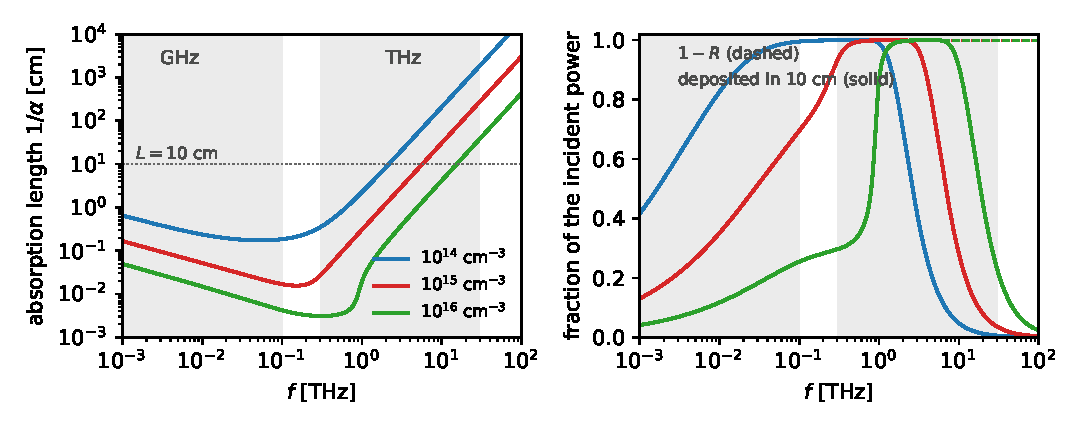
\includegraphics[width=0.86\textwidth]{chapters/env/fig_v5.pdf}
\caption{Pure Kr at 0.5~atm. Left: the absorption length against frequency for the three
densities, with the depth $L=10$~cm dotted; the shaded bands are the GHz range (1 to 100~GHz) and
the THz range (0.3 to 30~THz). Right: the fraction of the incident power that enters the gas,
$1-R$ (dashed), and the fraction deposited in the 10~cm (solid).}
\label{env:fig:spectrum}
\end{figure}

{\noindent}(3) \emph{GHz.} At $10^{15}$ and $10^{16}$~cm$^{-3}$ the gas is a mirror: it reflects 31
to 94\,\% between 2.45 and 95~GHz at 0.5~atm, 8 to 96\,\% over all pressures, and absorbs the
remainder within 0.04 to 1.1~mm of the front. At $10^{14}$~cm$^{-3}$ the collisions outrun the
cutoff and the wave gets in (43\,\% reflected at 2.45~GHz and 1\,\% at 95~GHz), but it is absorbed
in 1.8 to 4.2~mm (0.6 to 8.3~mm over the pressures and both gases): the front millimetres take
all of it and the rest of the gas nothing, since the deposition falls by $e^{\alpha L}$, at least
$10^{5}$, from front to back. \\ \\
\emph{THz.} The gas reflects at most 15\,\% (1~THz at
$10^{16}$~cm$^{-3}$) and nothing above 3~THz, and the absorption length runs from 0.2~mm to 2~m,
through the depth of the gas at 2.2, 5.7 and 15.4~THz for the three densities at 0.5~atm, and at
1.1 to 26.5~THz over the 18 cells. At 3~THz the 10~cm deposits 41, 97 and 100\,\% of the incident
power. Per electron the heating at a given intensity goes as $\nueff/(\omega^2+\nueff^2)$ by
Eq.~\eqref{env:eq:P-drude}, largest at GHz, where every electron heats as in a static field, and that
is exactly why the skin is thin: the first electrons take the whole wave. The GHz range would be
the right one only for a gas a millimetre thick at $10^{14}$~cm$^{-3}$ and 0.5~atm or more, where
95~GHz enters with 1\,\% reflection and is absorbed in 1.8 to 5.4~mm, or at densities below
$10^{12}$~cm$^{-3}$, where the cutoff falls to 9~GHz. Kr/F$_2$ changes the absorption lengths by at
most a factor 1.3 at 95~GHz and 3~THz and the reflections by at most 9 points.

\medskip
\noindent\textbf{In Summary:} For a gas deeper than a few millimetres the THz range is better: it
enters the gas and deposits over centimetres, where the GHz range reflects or skins. The best
frequency of Eq.~\eqref{env:eq:fA} lies on the transparent side of the peak, in the THz range at every
cell.


\section{The two gases}
\label{env:sec:results}

\subsection{The best frequencies}
\label{env:sec:table}
Table~\ref{env:tab:main} gives $\fbest$ at $L=10$~cm and 300~kW/cm$^3$ for the two gases,
with $\Te$ from Eq.~\eqref{env:eq:balance}. The flags come from the particle balance of
Sec.~\ref{env:sec:particles}.

\begin{table}[ht]
\centering
\caption{The best frequency in THz at $L=10$~cm and 300~kW/cm$^3$, with $\Te$ in eV in
parentheses, for the two gases. $^a$: the field's own ionization outruns the losses and
$n_e$ grows during the pulse. $^s$: the losses outrun it and a source must hold $n_e$.}
\label{env:tab:main}
\begin{tabular}{lccc}
\toprule
$n_e$ [cm$^{-3}$] & 0.1 atm & 0.5 atm & 2 atm\\
\midrule
\multicolumn{4}{l}{\emph{pure Kr}}\\
\tabinput{chapters/env/tab_envelope_v4_Kr.tex}
\addlinespace
\multicolumn{4}{l}{\emph{Kr + 2\,\% F$_2$}}\\
\tabinput{chapters/env/tab_envelope_v4_KrF2.tex}
\bottomrule
\end{tabular}
\end{table}

\subsection{The particle balance}
\label{env:sec:particles}
{\noindent}(1) The density is not the field's to choose. Direct ionization by the
electrons, at the rate $\nu_{\rm ion}=N\sum_jx_jk_{{\rm ion},j}$ from the thresholds at
14.0~eV (Kr) and 15.7~eV (F$_2$), makes electrons. Attachment to F$_2$ at
$\nu_{\rm att}=Nx_{{\rm F}_2}k_{\rm att}$ removes them, and so does recombination. For the
recombination every cation is taken as Kr$_2^+$ with the coefficient of Shiu and Biondi
\cite{env:ShiuBiondi1977},
\begin{equation}
\alpha_{\rm rec}=1.6\times10^{-6}\Big(\frac{300~{\rm K}}{\Te}\Big)^{0.55}~{\rm cm^3/s},\qquad
\nu_{\rm rec}=\alpha_{\rm rec}\,n_e,
\label{env:eq:rec}
\end{equation}
measured from 300 to 8400~K, 0.72~eV, and extrapolated here. The net rate is
$\nu_{\rm net}=\nu_{\rm ion}-\nu_{\rm att}-\nu_{\rm rec}$.
\\ \\
{\noindent}(2) Where $\nu_{\rm net}>0$ the density e-folds in $1/\nu_{\rm net}$, which is 2.4
to 5.2~ns at the four cells marked $^a$ (pure Kr at $10^{14}$~cm$^{-3}$, and Kr/F$_2$ at
$10^{14}$~cm$^{-3}$ and 0.1~atm). Where $\nu_{\rm net}<0$ a source must supply
$-\nu_{\rm net}n_e$ electrons per second, at the least at the ionization energy of krypton,
\begin{equation}
\boxed{\;P_{\rm src}\ge n_e\,(\nu_{\rm att}+\nu_{\rm rec}-\nu_{\rm ion})\times14.0~{\rm eV}.\;}
\label{env:eq:Psrc}
\end{equation}
In pure Kr, where recombination is the loss, that is 300 to 410~kW/cm$^3$ at $10^{15}$ and
41 to 49~MW/cm$^3$ at $10^{16}$~cm$^{-3}$. With 2\,\% F$_2$ the loss is attachment at
$5.8\times10^{7}$ to $1.3\times10^{10}$~s$^{-1}$, and the source needs 32 and 430~kW/cm$^3$ at
$10^{14}$~cm$^{-3}$ and 0.5 and 2~atm, 0.5 to 7.8~MW/cm$^3$ at $10^{15}$ and 46 to
470~MW/cm$^3$ at $10^{16}$~cm$^{-3}$. Neither gas holds $10^{16}$~cm$^{-3}$ at these powers,
and Kr/F$_2$ does not hold $10^{15}$ either.
\\ \\
{\noindent}(3) Pure Kr left to itself settles where its ionization balances
recombination, $\nu_{\rm ion}(\Te(P/n_e))=\alpha_{\rm rec}(\Te)\,n_e$, in $1/\nu_{\rm ion}=15$
to 19~ns: at $n_e=4.5$, 3.6 and $2.9\times10^{14}$~cm$^{-3}$ for 0.1, 0.5 and 2~atm
($\Te=2.0$, 1.6 and 1.4~eV), where $\fbest=2.1$, 3.7 and 6.1~THz. Over 100 to
500~kW/cm$^3$ that is $1.6$ to $6\times10^{14}$~cm$^{-3}$ and 1.5 to 7.2~THz.

\subsection{The power laws}
\label{env:sec:laws}
Fitted to the nine cells of each gas at 300~kW/cm$^3$,
\begin{equation}
\boxed{\;\fbest\approx C\,\Big(\frac{n_e}{10^{15}~{\rm cm^{-3}}}\Big)^{b}
\Big(\frac{p}{1~{\rm atm}}\Big)^{c}\Big(\frac{L}{10~{\rm cm}}\Big)^{1/2},\;}
\label{env:eq:law}
\end{equation}
with $C=7.6$~THz, $b=0.43$, $c=0.40$ for pure Kr within 5.1\,\%, and $C=7.1$~THz, $b=0.41$,
$c=0.37$ for Kr/F$_2$ within 8.6\,\%. From 100 to 500~kW/cm$^3$ the best frequency rises by at most a
factor 1.16 in pure Kr, through $\Te$: at $10^{15}$~cm$^{-3}$ and 0.5~atm it is 4.4, 7.1 and
8.7~THz for $\Te=1$, 2 and 4~eV. In Kr/F$_2$ the power moves it by up to a factor 3.4, at
$10^{15}$~cm$^{-3}$ and 2~atm, since at 100~kW/cm$^3$ the F$_2$ losses already hold the
electrons at 0.16~eV there.

\subsection{Fluorine against pure krypton}
\label{env:sec:f2}
{\noindent}(1) At a given $\Te$ the 2\,\% F$_2$ adds at most 4.6\,\% to the kernel \eqref{env:eq:nuea}, so
the frequency is the same wherever the krypton excitation takes the power: Kr/F$_2$ is within 2\,\%
of pure Kr at six cells ($\Te\ge1.2$~eV) and 9 to 18\,\% below it at $10^{15}$~cm$^{-3}$ and 2~atm and
at $10^{16}$~cm$^{-3}$ and 0.5 and 2~atm, where the F$_2$ losses hold the electrons in the Ramsauer
minimum.
\\ \\
{\noindent}(2) What F$_2$ changes is the closure. Attachment removes the electrons in 0.1 to 17~ns,
so a source must hold the density nearly everywhere, and from $10^{15}$~cm$^{-3}$ up the source's
power exceeds the field's and its electrons set $\Te$ (Secs.~\ref{env:sec:kinetic} and
\ref{env:sec:uncertainty}).

\medskip
\noindent\textbf{In Summary:} Pure Kr wants 1.1 to 3.8~THz at $10^{14}$~cm$^{-3}$, 3.0 to
10.1 at $10^{15}$ and 8.7 to 26.5~THz at $10^{16}$, and 2\,\% F$_2$ changes the frequency only where
its losses cool the electrons. The density is the source's choice wherever F$_2$ is present, and
neither gas holds $10^{16}$~cm$^{-3}$ at these powers.


\section{The kinetic check}
\label{env:sec:kinetic}
{\noindent}(1) The envelope takes the electrons as Maxwellian. A two-term kinetic
solution \cite{env:HP2005} of every cell, with the same cross sections, the elastic collisions
with the ions, electron--electron collisions in Landau's form, and the temporal-growth
model in which the electrons that attachment removes or ionization adds are replaced or
removed with the shape of the distribution, gives $\Te$ as two thirds of the mean energy
and the absorption from the complex mobility at the envelope's $\fbest$, from which the
kinetic $f_A$ follows with $\alpha\propto f^{-2}$.
\\ \\
{\noindent}(2) In pure Kr the kinetic $\Te$ is 0.94 to 1.35 times the envelope's and the
kinetic $\fbest$ 0.89 to 1.23 times it: the inelastic collisions deplete the tail that a
Maxwellian keeps, so the bulk must be hotter to lose the same power, most at
$10^{15}$~cm$^{-3}$. With 2\,\% F$_2$ the same holds at the four cells where the field
outweighs attachment, with $\fbest$ at 0.96 to 1.12 times the envelope. At the other five,
$10^{15}$~cm$^{-3}$ from 0.5~atm up and all of $10^{16}$, attachment takes 0.6 to 25 times the
field's power from the electrons, so the source that replaces them sets $\Te$, and the
growth model is no longer a field-heated plasma.

\medskip
\noindent\textbf{In Summary:} The Maxwellian envelope is good to $-11$ to $+23$\,\% in
frequency where the field sets the temperature. Where the source does, the temperature,
and with it the frequency, is the source's.


\section{The uncertainty of the result}
\label{env:sec:uncertainty}

\subsection{Propagation}
\label{env:sec:propagation}
{\noindent}(1) From Eq.~\eqref{env:eq:fA}, $\fbest\propto\nueff^{1/2}$, so that a fractional
change of the collision frequency moves the frequency by half of it, and a change of the
ions' term alone by half of its share $s_i=\nuei/\nueff$:
\begin{equation}
\boxed{\;\frac{\delta\fbest}{\fbest}=\frac12\,\frac{\delta\nueff}{\nueff},\qquad
\frac{\delta\fbest}{\fbest}=\frac{s_i}{2}\,\frac{\delta\nuei}{\nuei}.\;}
\label{env:eq:propagation}
\end{equation}
A change of $\Te$ acts through $\sigma_m(\Te)$: between 1 and 2~eV in pure Kr,
$\fbest\propto\Te^{0.70}$, and between 2 and 4~eV, $\Te^{0.31}$.
\\ \\
{\noindent}(2) Each cell gets a central value and one uncertainty, $\fbest\pm\delta$. With
the bands $[m_-,m_+]$, $[i_-,i_+]$, $[e_-,e_+]$ and $[x_-,x_+]$ of the four sources below
as factors on the envelope's value $f_{\rm env}$,
\begin{equation}
\boxed{\;\begin{aligned}
f_c&=f_{\rm env}\,\frac{m_-+m_+}{2}\,\frac{i_-+i_+}{2},\\
\frac{\delta}{f_c}&=\Big[\Big(\frac{m_+-m_-}{2}\Big)^2+\Big(\frac{i_+-i_-}{2}\Big)^2
+\Big(\frac{e_+-e_-}{2}\Big)^2+\Big(\frac{x_+-x_-}{2}\Big)^2\Big]^{1/2},
\end{aligned}\;}
\label{env:eq:delta}
\end{equation}
the half-widths added in quadrature as independent errors.

\subsection{The sources}
\label{env:sec:sources}
{\noindent}(M) \emph{The envelope against the kinetic solution.} The two models of
Sec.~\ref{env:sec:kinetic} bracket the answer: $m_\mp$ are the smaller and the larger of 1
and $f_{\rm kin}/f_{\rm env}$. The half-width is 0.2 to 12\,\% in pure Kr. At the five
source-set cells of Kr/F$_2$ the band is instead $\fbest$ over $\Te=1$ to 4~eV, 0.79 to 2.5
times the envelope, and its half-width, 27 to 62\,\%, stands in for (M).
\\ \\
{\noindent}(I) \emph{The electron--ion term against the measurements.} Turnbull et al.\
measured absorption fractions of 1 to 4\,\% in hydrogen and nitrogen--hydrogen plasmas
with an absolute uncertainty of ($-0.12$\,\%, $+0.07$\,\%), found their best shots
predicted to better than 10\,\%, and their models 16\,\% above the data on average without
the fitted screening factor \cite{env:Turnbull2023,env:Turnbull2024}. The electron--ion
absorption of Eqs.~\eqref{env:eq:nuT} and \eqref{env:eq:Lambda}, with the dynamic cutoff and the
exact Gaunt factor and no fitted factor, is 1.19 to 1.20 times their four hydrogen
measurements. Taking the measurements as right within 10\,\%, the ion term is 0.75 to
0.92 of the computed one, and Eq.~\eqref{env:eq:propagation} with the midpoint 0.84 gives
$i_\mp$: the half-width is 0.0 to 1.0\,\% in pure Kr, the most at $10^{16}$~cm$^{-3}$ and
0.1~atm, and up to 4.3\,\% at the cold cells, where the ions carry most of the absorption.
\\ \\
{\noindent}(E) \emph{The momentum-transfer cross section against swarm experiments.} The
atoms carry the absorption, so the cross section $\sigma_m$ of krypton is the input that matters,
and the electron drift velocity $W$ in a DC field is its experimental test: for $\omega\gg\nu$ the
absorption weights $\sigma_m$ as Eq.~\eqref{env:eq:nuea} does, and the drift velocity weights
$1/\sigma_m$ over the same electron energies, so that $\delta W/W\simeq-\delta\sigma_m/\sigma_m$. The
two-term equation \cite{env:HP2005} with the same Biagi set gives $W$ at each field strength of two
measurements in pure krypton, Pack, Voshall and Phelps \cite{env:Pack1962} at 300~K, as compiled by
Dutton \cite{env:Dutton1975}, and Nakamura \cite{env:Nakamura1991}, read from the figure of the published
abstract to about 3\,\%. Each measured point is placed at the electron temperature
$\Te=\tfrac23\langle\varepsilon\rangle$ of the computed swarm. Between 0.95 and 2.6~eV, the range of the
warm cells, the computed $W$ is 0.96 to 1.02 times Nakamura's (rms 1.8\,\%, 13 points) and 0.84
to 0.97 times Pack's (rms 8.4\,\%, 7 points), and the two experiments differ from each other by
as much. Below that range only Pack's data exist, and across the Ramsauer minimum the computed
$W$ is 0.80 to 1.20 times them. For each cell the points within $\pm25$\,\% of its $\Te$ give the
rms deviation of each experiment, and their quadratic mean $d$ weights the two experiments
equally. Since only the atoms' share $1-s_i$ of $\nueff$ depends on $\sigma_m$, and
$\fbest\propto\nueff^{1/2}$, the half-width is
\begin{equation}
\boxed{\;\frac{e_+-e_-}{2}=(1-s_i)\,\frac d2,\;}
\label{env:eq:swarm}
\end{equation}
1.4 to 4.0\,\% in pure Kr. The same deviation, taken as an uncertainty of $\sigma_m$, replaces an
assumed one: had $\sigma_m$ been taken as good to 10\,\%, Eq.~\eqref{env:eq:propagation} and the cells
recomputed with $\sigma_m\times0.9$ and $\times1.1$ give 3.7 to 5.0\,\% in pure Kr. Adding both would
count the cross section twice, so Eq.~\eqref{env:eq:delta} carries (E), and the 10\,\% figure stands as
a bound that the swarm data do not reach.

{\noindent}(X) \emph{The inelastic cross sections of krypton}, taken as good to 20\,\%,
move $\Te$ through Eq.~\eqref{env:eq:balance} and with it $\fbest$ by 1.0 to 1.7\,\% in pure Kr.

{\noindent}(D) \emph{The recombination coefficient}, $\pm10$\,\% as stated
\cite{env:ShiuBiondi1977}, moves the self-sustained density of pure Kr by $-4.0$ to $+4.6$\,\%
and its frequency by $\mp1.9$\,\%. Its extrapolation beyond 0.72~eV is not bounded.

\subsection{The result}
\label{env:sec:uresult}
Table~\ref{env:tab:uncert} gives $\fbest\pm\delta$ at the 18 cells with the four contributions.
In pure Kr $\delta/\fbest$ is 2 to 12\,\%, and (M) and (E) together carry most of $\delta^2$ at eight
of the nine cells. In Kr/F$_2$ it is 3 to
7\,\% at the four field-set cells and 27 to 62\,\% at the five source-set ones, where the
temperature the source chooses is the uncertainty.

{\small
\setlength{\tabcolsep}{4pt}
\begin{longtable}{llccccccc}
\caption{The best frequency with its uncertainty at every cell of Table~\ref*{env:tab:main},
and the four contributions to $\delta$ in per cent. $^t$: the source sets $\Te$, and the
half-width of $\fbest$ over $\Te=1$ to 4~eV stands in for (M).}\label{env:tab:uncert}\\
\toprule
gas & $n_e$ [cm$^{-3}$] & $p$ [atm] & $\fbest\pm\delta$ [THz] & $\delta$ [\%] & (M) & (I) & (E) & (X)\\
\midrule
\endfirsthead
\toprule
gas & $n_e$ [cm$^{-3}$] & $p$ [atm] & $\fbest\pm\delta$ [THz] & $\delta$ [\%] & (M) & (I) & (E) & (X)\\
\midrule
\endhead
\bottomrule
\endfoot
\tabinput{chapters/env/tab_uncert_v6.tex}
\end{longtable}}

\medskip
\noindent\textbf{In Summary:} The uncertainty of the best frequency is
Eq.~\eqref{env:eq:delta} from the Maxwellian envelope against the kinetic solution, the
electron--ion term against Turnbull's data, the momentum-transfer cross section against the
swarm measurements, and the inelastic cross sections. It is 2 to 12\,\% in pure Kr, since the
atoms carry the absorption, their cross section reproduces the measured drift velocities to a
few per cent, and the ion term that Turnbull's measurements test contributes at most 1\,\%, and it is the source's temperature wherever F$_2$ makes a
source necessary.


\section{A worked example}
\label{env:sec:example}
Pure Kr at $n_e=10^{15}$~cm$^{-3}$, $p=0.5$~atm, $P=300$~kW/cm$^3$ and $L=10$~cm, the central cell
of Table~\ref{env:tab:main}, carried through from the gas density to the recommended frequency.
\\ \\
{\noindent}(1) \emph{The gas and the power per electron.} $N=2.45\times10^{19}\times0.5=1.22\times10^{19}$
atoms per cm$^3$, and $P/n_e=3\times10^{5}~{\rm W\,cm^{-3}}/10^{15}~{\rm cm^{-3}}=1.87\times10^{9}$~eV/s
per electron.
\\ \\
{\noindent}(2) \emph{The temperature.} Equation~\eqref{env:eq:balance} balances at $\kB\Te=1.42$~eV:
the recoil of Eq.~\eqref{env:eq:Pel} takes $3.3\times10^{7}$~eV/s, 1.8\,\%, and krypton's levels take
$1.84\times10^{9}$~eV/s, the rest.
\\ \\
{\noindent}(3) \emph{The collision frequency.} The kernel \eqref{env:eq:nuea} gives
$\nuea=1.22\times10^{12}$~s$^{-1}$, 2.10 times the Drude mean $5.8\times10^{11}$~s$^{-1}$. For the
ions, Eq.~\eqref{env:eq:nuT} gives $\nuT=1.71\times10^{9}$~s$^{-1}$, $\eta_t=4.4$ puts the collisions in
the classical regime, $\Lambda=3.65$ where the Born logarithm would give 4.90, and
$\nuei=6.3\times10^{9}$~s$^{-1}$, 0.5\,\% of $\nueff=1.22\times10^{12}$~s$^{-1}$. So
$\nueff/2\pi=0.19$~THz.
\\ \\
{\noindent}(4) \emph{The cutoff and the reflection limit.} $f_{pe}=8.98~{\rm kHz}\times(10^{15})^{1/2}
=0.28$~THz, and $f_R=1.294f_{pe}=0.37$~THz without the collisions, 0.32~THz with them in
Eq.~\eqref{env:eq:optics}.
\\ \\
{\noindent}(5) \emph{The absorption length.} Equation~\eqref{env:eq:fA} with $n_e/10^{15}=1$,
$\nueff/10^{12}=1.22$ and $L/10~{\rm cm}=1$ gives $f_A=5.2\times(1.22)^{1/2}=5.73$~THz, and the exact
root of $\alpha L=1$ is 5.73~THz. So $\fbest=5.7$~THz, far above $f_R$. There $u=0.017$ and
$\alpha_L=2.2\times10^{-3}$, so the soft-photon kernel and the absence of Langdon's flattening both
hold.
\\ \\
{\noindent}(6) \emph{The field.} Equation~\eqref{env:eq:E0} gives $E_0=47.6$~kV/cm, an intensity of
3~MW/cm$^2$.
\\ \\
{\noindent}(7) \emph{GHz instead?} At 95~GHz, $\nueff/\omega=2.1$: the wave is in the collisional
skin, with an absorption length of 0.17~mm and 31\,\% reflected. At 2.45~GHz, 1.1~mm and 80\,\%
reflected. At 1~THz the gas is already transparent, $R=0$, but the absorption length is 3.0~mm and
the front centimetre takes everything. At 3~THz it is 2.7~cm. The depth of the gas is matched on
the transparent side, at 5.7~THz.
\\ \\
{\noindent}(8) \emph{The density.} Direct ionization runs at $\nu_{\rm ion}=1.6\times10^{7}$~s$^{-1}$
against recombination at $1.8\times10^{8}$~s$^{-1}$ (5.7~ns per electron), so this density decays
unless a source supplies at least 360~kW/cm$^3$ by Eq.~\eqref{env:eq:Psrc}, more than the field. Left to
itself at this pressure and power, pure Kr settles at $3.6\times10^{14}$~cm$^{-3}$ and
$\kB\Te=1.62$~eV in 17~ns, where $\fbest=3.7$~THz.
\\ \\
{\noindent}(9) \emph{The uncertainty.} The kinetic solution of Sec.~\ref{env:sec:kinetic} gives
$\kB\Te=1.80$~eV and $\fbest=6.7$~THz, 1.17 times the envelope, so (M) contributes a half-width
of 8.7\,\%; (I) 0.02\,\%, since the ions carry 0.5\,\%; (E) 1.7\,\%, from the 9 swarm points within
$\pm25$\,\% of 1.42~eV, where the computed drift velocity deviates from Nakamura's by 1.2\,\% rms and
from Pack's by 4.6\,\%, so that $d=3.3\,\%$; (X) 1.7\,\%. Equation~\eqref{env:eq:delta} gives
$\delta/\fbest=9.0\,\%$ about the midpoint:
\begin{equation}
\boxed{\;\fbest=6.2\pm0.6~{\rm THz}.\;}
\label{env:eq:example}
\end{equation}
\\ \\
{\noindent}(10) \emph{With 2\,\% F$_2$ at the same point.} $\kB\Te=1.37$~eV, F$_2$'s channels taking
26\,\% of the losses, and $\fbest=5.6$~THz, 2\,\% below pure krypton's. But attachment runs at
$6.1\times10^{8}$~s$^{-1}$, 1.6~ns per electron, the source must supply at least 1.7~MW/cm$^3$, six
times the field's power, and in the kinetic solution it takes 0.60 of the field's power from the
electrons, so it sets $\Te$ and the frequency is $6.6\pm2.5$~THz, 38\,\%.

\medskip
\noindent\textbf{In Summary:} At $10^{15}$~cm$^{-3}$, 0.5~atm and 300~kW/cm$^3$ in a 10~cm gas, the
best frequency is $6.2\pm0.6$~THz, Eq.~\eqref{env:eq:example}. The GHz range is out: 31 to 80\,\%
reflected and the rest absorbed in 0.2 to 1~mm. The density is not free: pure Kr at this
density needs a source of 360~kW/cm$^3$ or settles at $3.6\times10^{14}$~cm$^{-3}$, where it wants
3.7~THz, and with F$_2$ the source needs 1.7~MW/cm$^3$ and sets the temperature.


\section{Summary}
\label{env:sec:summary}
\noindent\textbf{In Summary:} The best frequency for inverse-bremsstrahlung heating of a
krypton laser gas is the one whose absorption length matches the depth of the gas,
Eq.~\eqref{env:eq:fbest}, and it is Eq.~\eqref{env:eq:fA}: the square root of the electron
density, of the collision frequency and of the depth. The collision frequency is that of
the atoms, Eq.~\eqref{env:eq:nuea}, which the ions supplement by a few per cent at
$10^{15}$~cm$^{-3}$ and by up to a quarter at $10^{16}$, and it depends on the electron
temperature that the power balance \eqref{env:eq:balance} sets, 0.95 to 2.6~eV where the
field sets it. Pure Kr wants $1.1\pm0.1$~THz at $10^{14}$~cm$^{-3}$ and 0.1~atm, rising as
$(n_ep)^{0.4}$ and $L^{1/2}$ to $27.9\pm1.7$~THz at $10^{16}$~cm$^{-3}$ and 2~atm, with 2 to
12\,\% uncertainty, and left to itself it runs at $1.6$ to $6\times10^{14}$~cm$^{-3}$ and
wants 1.5 to 7~THz. The THz range is the right one: across the spectrum the absorption
peaks at 0.05 to 0.50~THz, between the bands, and the GHz range either reflects, 31 to 94\,\%
from $10^{15}$~cm$^{-3}$ up, or is absorbed in a millimetre skin, while the THz range enters the
gas and deposits over centimetres. 2\,\% F$_2$ leaves the frequency alone wherever the
krypton excitation takes the power. But F$_2$ attaches the electrons in 0.1 to 17~ns, so a
source sets the density and, from $10^{15}$~cm$^{-3}$ up, the temperature, and the frequency
is then known only to the source's temperature, 27 to 62\,\%. Neither gas holds
$10^{16}$~cm$^{-3}$ at 100 to 500~kW/cm$^3$. At the worked example, pure Kr at
$10^{15}$~cm$^{-3}$ and 0.5~atm, the answer is $6.2\pm0.6$~THz.


\chapterappendix
\section{The numerical checks}
\label{env:app:checks}
A check script verifies every boxed result of these notes, in
their order, by an independent numerical route: the Drude optics against the exact
complex refractive index, the energy-weighted kernel \eqref{env:eq:nuea} against the
velocity-space integral \eqref{env:eq:nuea-general} by quadrature and against the $4/3$ of a
constant cross section, the rate \eqref{env:eq:rate} and the recoil loss \eqref{env:eq:Pel}
against quadrature and against the closed form of a step cross section, the Spitzer
prefactor, the Born and classical limits of the logarithm, the reflection limit
\eqref{env:eq:fR}, the closed form \eqref{env:eq:fA} against the exact root, the field
\eqref{env:eq:E0} and Langdon's parameter \eqref{env:eq:alphaL} against the solved cells, the
particle balance, the fits \eqref{env:eq:law}, the collisional-skin law \eqref{env:eq:skin}, the
swarm comparison \eqref{env:eq:swarm} with the drift velocities recomputed and the measured values read
from their data files, the combination \eqref{env:eq:delta}, and every step of the worked example of Sec.~\ref{env:sec:example}. It
reproduces every number printed in these notes to its last printed digit from the stored results of the calculation of the cells and of the swarm comparison, checks the quoted figures of Turnbull et al.\ against the text of
their papers, and checks the logical statements. It runs with \texttt{numpy} and \texttt{scipy}
under Python~3 in a few seconds from those stored results, which the scripts
behind them take about four minutes to produce. Table~\ref{env:tab:checks} is
written by the script itself. A quantitative check passes when its deviation is below
the tolerance stated in the script, a printed number when the script reproduces it to
its last printed digit, and a logical condition when it holds.

\begin{longtable}{L{4.0cm}cccc}
\caption{The numerical checks of these notes, by the equation, table or section they verify. The second column counts all checks of the row. The third gives the largest deviation among its quantitative checks, relative, or absolute for quantities near zero, and is empty when the row has none. The fourth counts the numbers printed in these notes that the script reproduces to their last printed digit, and the fifth the logical conditions.}\label{env:tab:checks}\\
\toprule
Equation & Checks & Largest deviation & Printed & Logical\\
\midrule
\endfirsthead
\toprule
Equation & Checks & Largest deviation & Printed & Logical\\
\midrule
\endhead
\bottomrule
\endfoot
Sec.~\ref*{env:sec:question} & 2 &  & 1 & 1\\
Eq.~(\ref*{env:eq:fbest}) & 5 &  & 2 & 3\\
Eq.~(\ref*{env:eq:drude-eps}) & 2 & $0$ &  & 1\\
Eq.~(\ref*{env:eq:optics}) & 10 & $1.3\times10^{-9}$ & 6 & 2\\
Eq.~(\ref*{env:eq:alpha}) & 2 & $1.0\times10^{-4}$ &  & \\
Eq.~(\ref*{env:eq:P-drude}) & 1 & $0$ &  & \\
Eq.~(\ref*{env:eq:drude-sigma}) & 1 & $0$ &  & \\
Eq.~(\ref*{env:eq:nuea}) & 8 & $1.7\times10^{-7}$ & 5 & \\
Sec.~\ref*{env:sec:atoms} & 1 &  & 1 & \\
Eq.~(\ref*{env:eq:Pel}) & 4 & $1.7\times10^{-7}$ & 2 & 1\\
Eq.~(\ref*{env:eq:nuT}) & 5 & $1.3\times10^{-3}$ & 2 & \\
Eq.~(\ref*{env:eq:Lambda1}) & 3 & $1.1\times10^{-9}$ & 1 & \\
Eq.~(\ref*{env:eq:Lambda}) & 4 & $4.2\times10^{-3}$ & 1 & 1\\
Sec.~\ref*{env:sec:ions} & 7 & $2.7\times10^{-6}$ & 6 & \\
Eq.~(\ref*{env:eq:nueff}) & 12 &  & 9 & 3\\
Sec.~\ref*{env:sec:leftout} & 2 &  & 1 & 1\\
Eq.~(\ref*{env:eq:alphaL}) & 4 & $5.7\times10^{-2}$ & 2 & 1\\
Eq.~(\ref*{env:eq:balance}) & 6 & $1.3\times10^{-13}$ & 3 & 1\\
Eq.~(\ref*{env:eq:rate}) & 3 & $8.3\times10^{-5}$ &  & \\
Sec.~\ref*{env:sec:temperature} & 21 &  & 19 & 2\\
Eq.~(\ref*{env:eq:E0}) & 6 & $2.7\times10^{-10}$ & 4 & 1\\
Eq.~(\ref*{env:eq:fR}) & 10 & $1.0\times10^{-13}$ & 7 & 1\\
Sec.~\ref*{env:sec:reflection} & 2 &  & 1 & 1\\
Eq.~(\ref*{env:eq:fA}) & 8 & $2.2\times10^{-3}$ & 5 & 2\\
Sec.~\ref*{env:sec:spectrum} & 42 &  & 36 & 6\\
Eq.~(\ref*{env:eq:skin}) & 5 & $0$ & 3 & 1\\
Table~\ref*{env:tab:spectrum} & 10 &  &  & 10\\
Table~\ref*{env:tab:main} & 19 &  &  & 19\\
Eq.~(\ref*{env:eq:rec}) & 6 &  & 3 & 3\\
Sec.~\ref*{env:sec:particles} & 36 &  & 33 & 3\\
Eq.~(\ref*{env:eq:Psrc}) & 4 &  & 1 & 3\\
Eq.~(\ref*{env:eq:law}) & 9 & $0$ &  & 3\\
Sec.~\ref*{env:sec:laws} & 7 &  & 6 & 1\\
Sec.~\ref*{env:sec:f2} & 7 &  & 5 & 2\\
Sec.~\ref*{env:sec:summary} & 15 &  & 14 & 1\\
Sec.~\ref*{env:sec:results} & 1 &  &  & 1\\
Sec.~\ref*{env:sec:kinetic} & 16 &  & 13 & 3\\
Eq.~(\ref*{env:eq:propagation}) & 3 & $3.9\times10^{-3}$ & 2 & \\
Eq.~(\ref*{env:eq:delta}) & 11 &  & 8 & 3\\
Sec.~\ref*{env:sec:sources} & 29 &  & 21 & 8\\
Eq.~(\ref*{env:eq:swarm}) & 23 & $0$ & 11 & 8\\
Sec.~\ref*{env:sec:uresult} & 7 &  & 6 & 1\\
Table~\ref*{env:tab:uncert} & 19 &  &  & 19\\
Sec.~\ref*{env:sec:example} & 22 & $0$ & 16 & 4\\
Eq.~(\ref*{env:eq:example}) & 5 & $0$ & 2 & 1\\
Appendix~\ref*{env:app:checks} & 4 &  &  & 4\\
\midrule
Total & 429 & & 258 & 126\\
\end{longtable}



\begin{thebibliography}{99}
\raggedright
\bibitem{env:Atzeni2004} S.~Atzeni and J.~Meyer-ter-Vehn, \emph{The Physics of Inertial Fusion}
(Oxford University Press, Oxford, 2004), doi:\href{https://doi.org/10.1093/acprof:oso/9780198562641.001.0001}{10.1093/acprof:oso/9780198562641.001.0001}.
\bibitem{env:Pitchford2016} L.~C.~Pitchford \emph{et al.}, Plasma Process. Polym. \textbf{14}, 1600098 (2016),
doi:\href{https://doi.org/10.1002/ppap.201600098}{10.1002/ppap.201600098} (LXCat, Biagi-v7.1 database).
\bibitem{env:Morgan1992} W.~L.~Morgan, Plasma Chem. Plasma Process. \textbf{12}, 449 (1992),
doi:\href{https://doi.org/10.1007/BF01447254}{10.1007/BF01447254} (LXCat, SIGLO database).
\bibitem{env:HP2005} G.~J.~M.~Hagelaar and L.~C.~Pitchford, Plasma Sources Sci. Technol. \textbf{14}, 722 (2005),
doi:\href{https://doi.org/10.1088/0963-0252/14/4/011}{10.1088/0963-0252/14/4/011}.
\bibitem{env:Low1958} F.~E.~Low, Phys. Rev. \textbf{110}, 974 (1958),
doi:\href{https://doi.org/10.1103/PhysRev.110.974}{10.1103/PhysRev.110.974}.
\bibitem{env:KrollWatson1973} N.~M.~Kroll and K.~M.~Watson, Phys. Rev. A \textbf{8}, 804 (1973),
doi:\href{https://doi.org/10.1103/PhysRevA.8.804}{10.1103/PhysRevA.8.804}.
\bibitem{env:KarzasLatter1961} W.~J.~Karzas and R.~Latter, Astrophys. J. Suppl. \textbf{6}, 167 (1961),
doi:\href{https://doi.org/10.1086/190063}{10.1086/190063}.
\bibitem{env:vanHoof2014} P.~A.~M.~van~Hoof, R.~J.~R.~Williams, K.~Volk, M.~Chatzikos, G.~J.~Ferland, M.~Lykins,
R.~L.~Porter and Y.~Wang, Mon. Not. R. Astron. Soc. \textbf{444}, 420 (2014),
doi:\href{https://doi.org/10.1093/mnras/stu1438}{10.1093/mnras/stu1438}.
\bibitem{env:DawsonOberman1962} J.~Dawson and C.~Oberman, Phys. Fluids \textbf{5}, 517 (1962),
doi:\href{https://doi.org/10.1063/1.1706652}{10.1063/1.1706652}.
\bibitem{env:Turnbull2023} D.~Turnbull \emph{et al.}, Phys. Rev. Lett. \textbf{130}, 145103 (2023),
doi:\href{https://doi.org/10.1103/PhysRevLett.130.145103}{10.1103/PhysRevLett.130.145103}.
\bibitem{env:Turnbull2024} D.~Turnbull \emph{et al.}, Phys. Plasmas \textbf{31}, 063304 (2024),
doi:\href{https://doi.org/10.1063/5.0203446}{10.1063/5.0203446}.
\bibitem{env:Langdon1980} A.~B.~Langdon, Phys. Rev. Lett. \textbf{44}, 575 (1980),
doi:\href{https://doi.org/10.1103/PhysRevLett.44.575}{10.1103/PhysRevLett.44.575}.
\bibitem{env:Pack1962} J.~L.~Pack, R.~E.~Voshall and A.~V.~Phelps, Phys. Rev. \textbf{127}, 2084 (1962),
doi:\href{https://doi.org/10.1103/PhysRev.127.2084}{10.1103/PhysRev.127.2084}.
\bibitem{env:Dutton1975} J.~Dutton, J. Phys. Chem. Ref. Data \textbf{4}, 577 (1975),
doi:\href{https://doi.org/10.1063/1.555525}{10.1063/1.555525}.
\bibitem{env:Nakamura1991} Y.~Nakamura, Meeting Abstracts of the Physical Society of Japan, 1991 autumn meeting,
abstract 27p-ZA-3, p.~103 (1991), doi:\href{https://doi.org/10.11316/jpsgaiyoa.1991.4.0_103}{10.11316/jpsgaiyoa.1991.4.0\_103}.
\bibitem{env:ShiuBiondi1977} Y.-J.~Shiu and M.~A.~Biondi, Phys. Rev. A \textbf{16}, 1817 (1977),
doi:\href{https://doi.org/10.1103/PhysRevA.16.1817}{10.1103/PhysRevA.16.1817}.
\end{thebibliography}
\endgroup

% Chapter qib: the note of October 12, 2026, assembled for the compendium -- do not edit by hand
\chapter{The best frequency for inverse bremsstrahlung in excimer laser gases: a krypton fill, the measured 5s to 5p rate, and the pulse}\label{qib:chapter}
\notedate{October 12, 2026}
\begingroup
\fontencoding{T1}\selectfont
\section{The question and the answer}
\label{qib:sec:answer}

A wave of frequency $f$ heats the electrons of an excimer laser gas by inverse bremsstrahlung. To deposit a power
density $P$ evenly through a layer of depth $L$, it has to be absorbed over that depth and not reflected at the
surface. The best frequency $f_{\rm best}$ is the frequency that does both, defined in Section~\ref{qib:sec:model}. It
depends on the electrons through their temperature and density and on the atoms and ions they collide with, and
the field that heats the electrons also excites the gas. The excited atoms are ionized by a second electron at
under a third of the energy the ground state needs, they ionize each other and the krypton, and they trade energy
with the electrons both ways. This note follows them inside both balances of the electrons, the balance of their
number and the balance of their energy, at every point of a table of three fills, two buffered and one of krypton
with 0.5~\% F$_2$, five pressures and five electron densities, 75 points in all, and it does four things the
earlier form of the calculation could not.

First, the excitation of krypton's 5s levels to 5p, the rate that carries most of the cooling of the electrons,
is taken from the measured cross sections of Jung et al.\ \cite{qib:Jung2005,qib:Jung2006} rather than from a discharge
model's fit, and the 5p manifold radiates to 5s at the measured lifetimes \cite{qib:Dzierzega2000}. Second, the
krypton fill is added, with no buffer gas. Its best frequency lies 1.04 to 1.20 times the argon fill's at the
same pressure and density, 1.05 to 8.8~THz at 0.1~atm and 3.8 to 26.9~THz at 2~atm, with its electrons at 0.94
to 2.44~eV, and the beam holds the density at 11 of its 25 points. With the measured cross section the neon fill
lies at 0.933 to 0.997 and the argon fill at 0.646 to 0.995 of the calculation without excited atoms. The fit in
place of the measurement raises the best frequency by up to 5~\%, the 5p rung's electron collisions left out raise
it by up to 1.46 times, and the return of 5p to 5s by collisions, raised from the estimate used here to the one
measured total loss rate of a 5p level \cite{qib:Gazeli2021}, lowers it by up to 13~\% at the dense krypton points and
the electron temperature there by 19~\%: that return rate is now the largest uncertainty of the answer. Third, the
calculation is marched in time through a pulse of 1~$\mu$s at three points, with the F$_2$ burning and the density
following its own balance. The steady table is the state of the first 100~ns at $10^{15}$~cm$^{-3}$ and of the
first 10~ns at $10^{16}$~cm$^{-3}$: the attachment that holds the density also burns the F$_2$, which is gone in
0.36 to 0.38~$\mu$s at $10^{15}$~cm$^{-3}$ and in 35~ns at $10^{16}$~cm$^{-3}$, after which the density runs up
3.7 to 6.8 times to where the beam's pairs balance recombination, the electrons cool to 0.53 to 0.54~eV and the
best frequency moves, by $-18$ and $-6$~\% at $10^{15}$~cm$^{-3}$ and by 2.8 times at $10^{16}$~cm$^{-3}$. Fourth, the
kinetic solver is checked against a second solver of the same equation, written independently for a time-domain
model of the KrF laser: at seven states from $10^{12}$ to $10^{16}$~cm$^{-3}$ the two agree within 0.2~\% in the
electrons' mean energy and in the wave's absorbed power, and the two full models, started from the same cold seed
under the same wave, decay the plasma at rates 1~\% apart with electrons 0.3~\% apart in temperature.

\section{The gas, the electrons and the best frequency}
\label{qib:sec:model}

\paragraph{The table.}
The three fills are Ne/Kr/F$_2$ in the mole fractions 0.948/0.05/0.002, Ar/Kr/F$_2$ in 0.597/0.4/0.003 and
Kr/F$_2$ in 0.995/0.005, at 300~K and pressures of 0.1, 0.2, 0.5, 1 and 2~atm. The electron density $n_e$ is
$10^{14}$, $3\times10^{14}$, $10^{15}$, $3\times10^{15}$ or $10^{16}$~cm$^{-3}$, and the field deposits
$P=300$~kW/cm$^3$ in a layer of depth $L=10$~cm. At each of these 75 points the frequency runs over 13 values, five
per decade from 0.1 to 25.1~THz.

\paragraph{The electrons.}
The electrons' energy distribution $F(\epsilon)$ solves the two-term Boltzmann equation in the oscillating field
\cite{qib:HP2005}, with the cross sections of Biagi's database for neon, argon, krypton and F$_2$ \cite{qib:LXCat},
electron--electron collisions, and collisions with the cations through the Coulomb cross section
$\pi\,(e^2/4\pi\epsilon_0\epsilon)^2\Lambda(\epsilon,\omega)$. The logarithm $\Lambda$ is the quantum one of
Turnbull et al.\ for the photon energy $\hbar\omega$ \cite{qib:T23,qib:T24}, cut off at the ion-sphere radius of the
cations. The field's amplitude is set so that the electrons absorb $P$. The electrons' complex mobility
$\mu(\omega)$ gives the conductivity $\sigma=n_ee\mu$ and the dielectric function
$\varepsilon=1+i\sigma/\epsilon_0\omega$, and from them the absorption coefficient and the reflection at normal
incidence,
\begin{equation}
\alpha=\frac{2\omega}{c}\,{\rm Im}\sqrt{\varepsilon},\qquad
R=\left|\frac{1-\sqrt{\varepsilon}}{1+\sqrt{\varepsilon}}\right|^2 .
\label{qib:eq:optics}
\end{equation}
$\alpha$ falls with $f$ once $\omega$ exceeds the collision and plasma frequencies. $f_A$ is the frequency at
which $\alpha L=1$, so that the wave is absorbed over the layer, and $f_R$ the lowest at which $R\le0.05$. The
best frequency is
\begin{equation}
f_{\rm best}=\max\left(f_A,\,f_R\right),
\label{qib:eq:fbest}
\end{equation}
both found by interpolating $\ln\alpha$ and $\ln R$ in $\ln f$ between the frequencies of the scan.

\paragraph{The ions and how the density is held.}
Electrons are lost to attachment on F$_2$ and to dissociative recombination on molecular cations. The two buffered
fills have five cations each, the atomic and the molecular ion of the buffer gas, the heteronuclear ion of the
buffer with krypton, Kr$^+$ and Kr$_2^+$, and the krypton fill has Kr$^+$ and Kr$_2^+$. They are made by the
field's ionization of each gas and by an electron beam, they convert into one another, and they recombine with the
electrons and with F$^-$, through the reactions of Table~\ref{qib:tab:ionrows} in Appendix~\ref{qib:app:rows}. The
recombination with F$^-$ turns over with pressure, as the three-body capture calculations that Kannari et al.\
review do \cite{qib:Kannari1985}, and the other charges screen each pair, which multiplies it here by
$S_c=1/(1+R_c/\lambda_D)$ with $R_c=2e^2/(3\cdot4\pi\epsilon_0kT_g)$ and $\lambda_D$ the Debye length of all the
charges at the gas temperature $T_g$. Where the ionization falls short of the losses, the beam makes up the
difference and holds $n_e$. Its electrons enter with the energy spectrum of the slow secondaries of a fast beam,
whose mean is 4.506~eV, and they are marked $b$ where they bring more than a third of the absorbed power. Where
the ionization exceeds the losses, the field multiplies the electrons at the net rate $g$, and the point is marked
$a$ where $g$ exceeds one $e$-fold in the pulse of 1~$\mu$s. A point marked $a$ is not steady over the pulse, and
its best frequency is that of the density it passes through.

\section{The excited atoms}
\label{qib:sec:ladder}

\paragraph{The levels.}
The field excites krypton into its four 5s levels and into 5p and the levels above. They are followed as two
species, Kr$^*$ for the 5s levels and Kr$^{**}$ for 5p and above, each standing at the energy of its lowest level,
9.915 and 11.30~eV, so that no excitation booked into a species creates energy. The buffer gas is followed the same
way, Ar$^*$ at argon's lowest 4s level, 11.548~eV, and Ne$^*$ at neon's lowest 3s level, 16.619~eV, and four
excited dimers form from these atoms, mostly in three-body collisions, Kr$_2^*$, Ar$_2^*$, ArKr$^*$ and Ne$_2^*$.
The krypton fill carries Kr$^*$, Kr$^{**}$ and Kr$_2^*$. Every energy is a formation energy above the ground-state
atoms, Table~\ref{qib:tab:levels}. Those of the atoms lie within 0.005~eV of the levels and ionization limits of the
NIST database \cite{qib:NISTASD}, those of Kr$_2^+$ and Ar$_2^+$ follow from the measured binding of the two ions
\cite{qib:Ng1977}, and the others are taken as the table gives them.

\begin{table}[!tbp]
\centering
\caption{The levels whose energy reaches the electrons, as formation energies above the ground-state atoms, in eV.}
\label{qib:tab:levels}
\small
\begin{tabular}{@{}l r L{8.2cm}@{}}
\toprule
species & energy & origin \\
\midrule
\tabinput{chapters/qib/tab_v4_levels.tex}
\bottomrule
\end{tabular}
\end{table}

The field makes Kr$^*$ and Kr$^{**}$ through the excitation cross sections of the Boltzmann equation, the 5s group
into Kr$^*$ and every higher group into Kr$^{**}$, and the buffer's excitations into its own species. The beam
shares its energy between the gases by their stopping powers for fast electrons, from Bethe's formula at 600~keV
with mean excitation energies of 137, 188, 352 and 115~eV for Ne, Ar, Kr and F$_2$, and makes one ion pair per
36.6~eV in neon \cite{qib:Lee1989}, 26.2~eV in argon and 32~eV in F$_2$ \cite{qib:Kannari1985}, and 24.2~eV in krypton,
where Kannari et al.\ print 24.3. With each pair it makes 0.305 excited atoms in neon and 0.284 in argon, the
energies per pair of Lee et al.\ over their energies per excited atom, 120 and 93~eV \cite{qib:Lee1989}, and 0.28 in
krypton \cite{qib:Kannari1985}. The recombination of the molecular cations leaves an excited atom behind. The excited
atoms are lost to F$_2$, which turns Kr$^*$ into KrF$^*$ at $8.47\times10^{-10}$~cm$^3$\,s$^{-1}$, the mean of
three measurements, with a yield of 0.90 \cite{qib:Velazco1976,qib:Ueda1984}, to the three-body formation of dimers, to
radiation, to Penning ionization, and to the electrons. Tables~\ref{qib:tab:hrows} and \ref{qib:tab:ionrows} of
Appendix~\ref{qib:app:rows} list every reaction between heavy particles with its rate and its source, and
Table~\ref{qib:tab:erows} the electron collisions. Each species stands at the steady state of its balance, solved for
all of them at once at the electrons' distribution. Where the field multiplies the electrons at the rate $g$, every
density grows with them, the ions as the excited atoms, and each species is diluted at $gn$ on top of its losses.

\begin{table}[!htbp]
\centering
\caption{The electron collisions of the excited atoms as the Boltzmann equation carries them. The rate is the
source's in cm$^3$\,s$^{-1}$ with $T_e$ in eV, $E_0$ the onset of the cross section of Eq.~(\ref*{qib:eq:sigma}) in eV,
and $\Delta$ the energy the electron loses, negative where it gains. The standing says whether the rate is measured,
printed by its source from elsewhere, calculated, the value of a related process, estimated, or detailed balance.}
\label{qib:tab:erows}
\footnotesize
\setlength{\tabcolsep}{3pt}
\begin{tabular}{@{}L{3.6cm} L{3.7cm} r r L{1.6cm} L{3.4cm}@{}}
\toprule
reaction & rate & $E_0$ & $\Delta$ & standing & source \\
\midrule
\tabinput{chapters/qib/tab_v4_erows.tex}
\bottomrule
\end{tabular}
\end{table}

\paragraph{The 5s to 5p excitation is measured.}
Jung et al.\ measured the cross sections for electron-impact excitation out of krypton's two metastable 5s
levels, $1s_5$ and $1s_3$ in Paschen's notation, into each of the ten 5p levels, from 2 to 300~eV, with
uncertainties of 35~\% for $1s_5$ and 40~\% for $1s_3$ \cite{qib:Jung2005,qib:Jung2006}. The cross section used here for
Kr$^*\to$ Kr$^{**}$ is their sum over the ten 5p levels, lumped over the 5s manifold by statistical weight,
$1s_5:1s_4:1s_3:1s_2=5:3:1:3$, with each unmeasured resonance level taken as its core partner, $1s_4$ as $1s_5$
and $1s_2$ as $1s_3$, since the core-preserving cross sections scale with the optical oscillator strengths. Each
level's cross section is zero below its threshold, rises linearly to the first tabulated point, follows the table
log-log between the points, and falls as $1/\epsilon$ past the last. Its onset on the ladder is the gap
between the lumped levels, 1.385~eV. On Maxwellians this cross section gives 1.36 times the rate of the discharge
model's fit that Kannari et al.\ print \cite{qib:Kannari1985,qib:JacobMangano1976} at the coldest electrons of the table,
0.87~eV, and 0.92 times at the hottest, 4.69~eV, differences at or inside the measurement's own uncertainty. The
fit is kept as the upper end of a band, Section~\ref{qib:sec:limits}.

\paragraph{The 5p manifold returns to 5s three ways.}
Kr$^{**}$ gives its energy back to the electrons in superelastic collisions, the detailed balance of the
excitation, and it returns to 5s by radiation and in collisions with the gas. The ten 5p levels radiate to the 5s
levels in the near infrared, on lines that end on the 5s levels and are not trapped, with the lifetimes that
Dzierzega et al.\ derive from the beam-gas-laser measurements of six of the levels, 23.1 to 38.1~ns
\cite{qib:Dzierzega2000}. The lumped manifold decays at the $2J+1$-weighted mean of their rates, one lifetime of
29.0~ns, and the 1.385~eV leaves as light. The return by collisions is the estimate of
$1.0\times10^{-10}$~cm$^3$\,s$^{-1}$ that Kannari et al.\ mark as such for Kr$^{**}$ + Ar \cite{qib:Kannari1985},
used for every partner. One measurement in krypton exists: Gazeli et al.\ measured the total loss rate of the
$5p'[3/2]_2$ level in krypton at 300~K, $(1.7\pm0.2)\times10^{-10}$~cm$^3$\,s$^{-1}$, without resolving its
product \cite{qib:Gazeli2021}. It bounds the return of the lumped manifold from above and is run as the upper end of
a band. The level-resolved rates of Whitehead et al.\ \cite{qib:Whitehead1995} would settle it and are not used
here. At the krypton fill at 1~atm and $10^{15}$~cm$^{-3}$, at 10~THz, the manifold returns 84~\% by collisions,
15~\% superelastically and 1.2~\% by radiation.

\paragraph{Stepwise ionization has no measurement.}
No measurement of the ionization of krypton's 5s levels by electrons was found, as a cross section or as a rate.
Kannari et al.\ print $7.00\times10^{-8}\,T_e^{0.68}e^{-4.04/T_e}$~cm$^3$\,s$^{-1}$ for it from Vriens's
binary-encounter calculation \cite{qib:Kannari1985,qib:Vriens1965}, and Johnson and Hunter print $4.8\times10^{-8}$ from
the same calculation \cite{qib:JH1980}. This note takes Kannari's fit. The stepwise ionization of Ar$^*$ has only a
transplanted law, that of Chen et al.\ for the higher of their two excited argon species
\cite{qib:Chen2025} at argon's 4s binding energy. In the calculation with Kannari's 5s to 5p fit, a stepwise rate
2.1 to 2.3 times Kannari's, or none at all, moved the best frequency by less than 1.5~\%, so the answer does not
rest on this rate and no band is run on it here.

\section{The excited atoms inside the electrons' balances}
\label{qib:sec:loop}

\paragraph{Every electron collision of an excited atom is a process of the Boltzmann equation.}
Each excited species enters the Boltzmann equation as a gas of its own, at the mole fraction its balance gives,
with every collision of an electron with it that Table~\ref{qib:tab:erows} lists. A rate fitted as $k=A\,T^B e^{-E/T}$
becomes the cross section
\begin{equation}
\sigma(\epsilon)=C\,\frac{(\epsilon-E_0)^{B+1/2}}{\epsilon}\quad(\epsilon>E_0),\qquad
C=\frac{A\sqrt{\pi}}{2\gamma\,\Gamma(B+3/2)},
\label{qib:eq:sigma}
\end{equation}
with $\gamma=(2e/m_e)^{1/2}$, whose rate over a Maxwellian of temperature $T$ is exactly $A\,T^Be^{-E_0/T}$. The
electron loses in it the energy $\Delta$ of the reaction on the ladder of formation energies of
Table~\ref{qib:tab:levels}. An electron below $\Delta$ cannot pay it, so the onset $E_0$ is the larger of the fit's $E$
and $\Delta$. Where the fit's $E$ lies above $\Delta$ the printed rate is kept and the electron loses $\Delta$.
Where it lies below, the onset moves up to $\Delta$, which lowers the rate on a Maxwellian by $e^{-(\Delta-E)/T}$.
A constant rate $k$ is the cross section $k/\gamma\sqrt{\epsilon}$, and a measured cross section enters as it is,
above the ladder's gap.

\paragraph{De-excitation by detailed balance.}
In a superelastic collision the electron gains the energy $\Delta$ of the level it empties. Its cross section
follows from that of the excitation it reverses by detailed balance \cite{qib:KR1921},
\begin{equation}
\sigma_{\downarrow}(\epsilon)=\frac{g_l}{g_u}\,\frac{\epsilon+\Delta}{\epsilon}\,\sigma_{\uparrow}(\epsilon+\Delta),
\label{qib:eq:db}
\end{equation}
with $g_l$ and $g_u$ the statistical weights of the lower and the upper level. Over a Maxwellian its rate is
$(g_l/g_u)\,e^{\Delta/T}$ times that of the excitation, and when the electrons are in equilibrium with the excited
atoms the two flows cancel. The Boltzmann operator places the electron $\Delta$ above the energy it had, so that
the equation is no longer solved from the top of the energy grid down and is solved as one linear system.

\paragraph{The electrons that the excited atoms set free.}
Penning ionization, between two excited atoms or dimers or between one of them and ground-state krypton, releases
an electron with the energy that the reaction leaves on the ladder, from 2.1 to 12.0~eV. These electrons enter the
Boltzmann equation as a source at their release energy, each in a band 0.2~eV wide.

\paragraph{The two closures.}
The Boltzmann equation is solved in steady state with a source of electrons. Where the beam holds the density, the
source is the beam's slow secondaries and the Penning electrons, mixed in proportion to their rates, and the rate
of injection per electron is what the losses leave over,
\begin{equation}
s=N\left(k_{\rm att}+k_{\rm rec}-k_{\rm ion}\right)=\frac{S_{\rm beam}+S_{\rm pen}}{n_e},
\label{qib:eq:held}
\end{equation}
with $N$ the gas density and $k_{\rm ion}$ the ionization of every gas of the equation, the excited ones among
them. Where the field multiplies the electrons at the rate $g$, the Penning electrons are the source and $g$ enters
as a loss from every energy in proportion to the electrons there, the dilution that growth brings, set so that
\begin{equation}
N\left(k_{\rm att}+k_{\rm rec}-k_{\rm ion}\right)+g=\frac{S_{\rm pen}}{n_e}.
\label{qib:eq:grow}
\end{equation}
Without a source the second closure is the growth model of the two-term equation \cite{qib:HP2005}. It leaves out the
share of the growth term in the anisotropic part of the distribution, which is of the order of $g/\nu_m$, the
growth rate over the momentum-transfer frequency, below $3\times10^{-3}$ at every growing point. The cations
follow the same particle balance, with the excited atoms' stepwise electrons added to the ionization of their
ground gas and the dimers' and the Penning electrons to their own cations.

\paragraph{The loop.}
Each round solves the Boltzmann equation with the excited atoms at their current mole fractions, then their
balance with the rates over the new distribution, then the ions, and sets the closure and the source of the next
round. The mole fractions are relaxed in their logarithm, and the loop ends when they, the ions and the beam's or
the growth rate change by less than $2\times10^{-3}$ between two rounds and the closure no longer changes. A
growth rate's change is measured against the larger of itself and $10^6$~s$^{-1}$, one $e$-fold in the pulse,
below which a growth rate multiplies nothing and its relative change says nothing. At the boundary between the
closures the two can alternate from round to round, with the beam's rate alternating between zero and a finite
value and the excited atoms differing by up to 1~\% between the two states, which is one and the same plasma within
that: a point whose excited atoms and ions have settled within ten tolerances and whose closure has alternated
for three rounds is accepted and flagged as a boundary point. It took 3 to 72 rounds per point, the most at the
one boundary cell of Section~\ref{qib:sec:limits}. Each frequency starts from the state of the one below it. The
electrons and the excited atoms book the same energy for every collision, which Appendix~\ref{qib:app:checks} tests
row by row as an identity.

\section{Results}
\label{qib:sec:results}

\paragraph{The table.}
Table~\ref{qib:tab:fbest} and Figure~\ref{qib:fig:fbest} give the best frequency at the 75 points with the excited atoms
inside the electrons' balances and the measured 5s to 5p cross section, and Table~\ref{qib:tab:compare} of
Appendix~\ref{qib:app:compare} every point with its electron temperature, its marks, the mole fraction of Kr$^*$, the
net energy the excited atoms take from the electrons, and the bands of Section~\ref{qib:sec:limits}. One cell of the
krypton fill, 0.5~atm and $10^{14}$~cm$^{-3}$, is a marginal plasma whose two closures alternate at most of its
frequencies, with the excited atoms moving by more than the boundary rule allows: 9 of its 13 frequencies closed,
4 of them at the flipping boundary, and the cell is reported incomplete, blank in the table and the figure and left
out of the bands.

\begin{table}[!tbp]
\caption{The best frequency $f_{\rm best}$ in THz at $L=10$~cm and 300~kW/cm$^3$ with the excited atoms inside the
electrons' balances. Marked $a$ where the field multiplies the electrons more than $e$-fold in the pulse of
1~$\mu$s, and $b$ where the beam's electrons bring more than a third of the absorbed power.}
\label{qib:tab:fbest}
\centering
\begin{tabular}{llrrrrr}
\toprule
fill & $p$ [atm] & $n_e=10^{14}$ & $3\times10^{14}$ & $10^{15}$ & $3\times10^{15}$ & $10^{16}$~cm$^{-3}$\\
\midrule
\tabinput{chapters/qib/tab_v4_fbest.tex}
\bottomrule
\end{tabular}
\end{table}

\begin{figure}[!tbp]
\centering
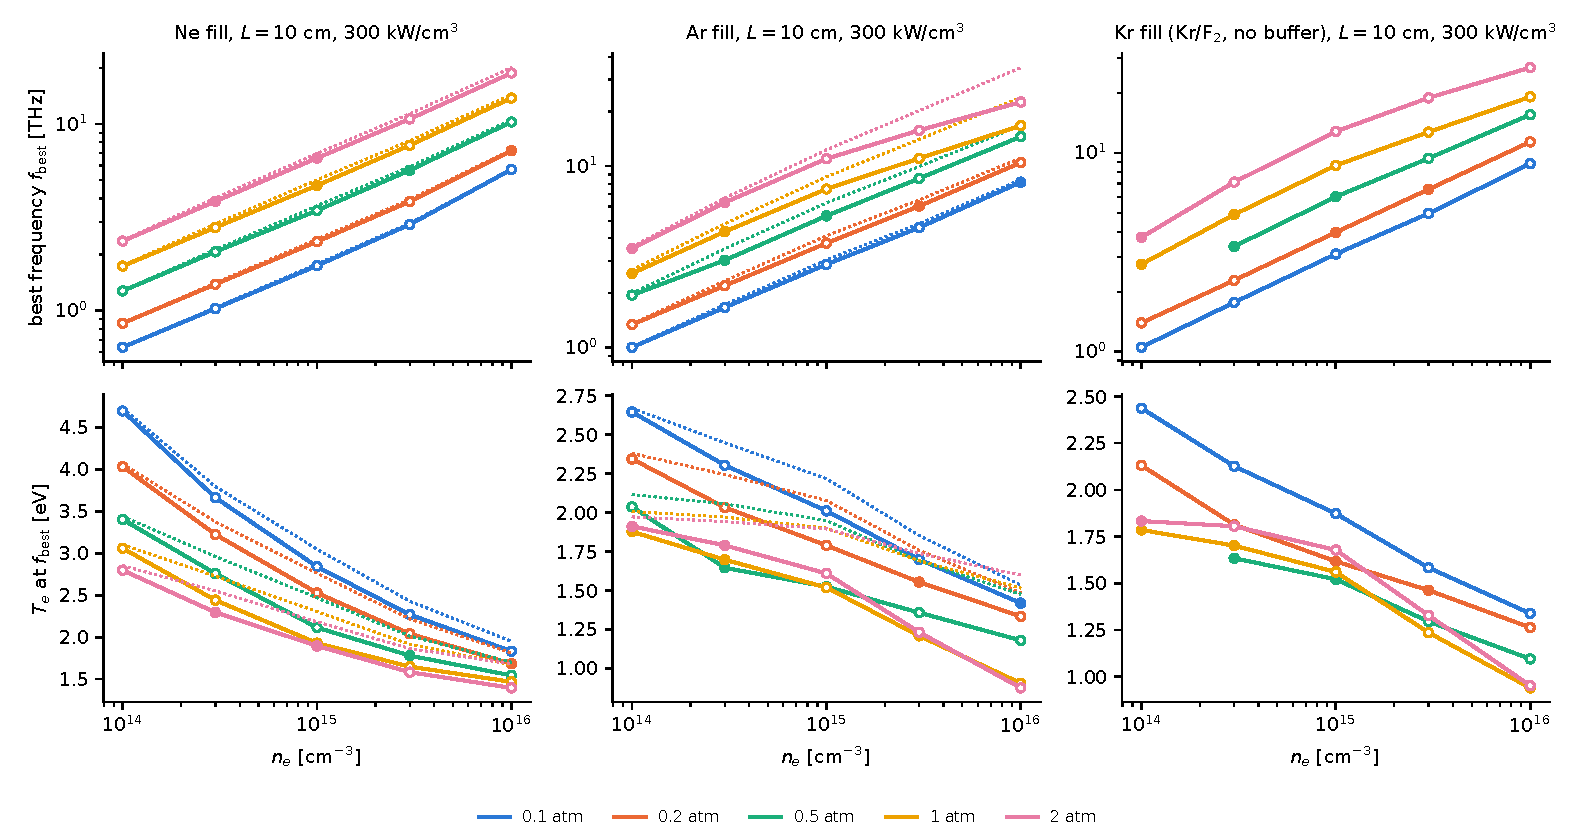
\includegraphics[width=\textwidth]{chapters/qib/fig_v4_fbest.pdf}
\caption{The best frequency at $L=10$~cm and 300~kW/cm$^3$ against $n_e$, top, and the electron temperature
$2\langle\epsilon\rangle/3$ there, bottom, with the excited atoms as solid lines and, for the two buffered fills,
without them dotted. An open marker is a point marked $a$ or $b$ in Table~\ref{qib:tab:fbest}. The krypton fill's cell
at 0.5~atm and $10^{14}$~cm$^{-3}$ is left blank.}
\label{qib:fig:fbest}
\end{figure}

\paragraph{The krypton fill against the argon fill.}
At the same pressure and density the krypton fill's best frequency lies 1.04 to 1.20 times the argon fill's, the
least at 0.2~atm and $3\times10^{14}$~cm$^{-3}$ and the most at 2~atm and $3\times10^{15}$~cm$^{-3}$. The reason
is the collision frequency. Above the collision frequency $\alpha$ falls as $\nu_m/\omega^2$, so the frequency at
which $\alpha L=1$ scales as the square root of the effective momentum-transfer frequency
$\nu_m=\omega\mu_r/\mu_i$, the ratio of the real to the imaginary part of the mobility times $\omega$. At the best
frequencies $\nu_m$ of the krypton fill is 1.08 to 1.52 times the argon fill's, and its square root gives the ratio
of the best frequencies within 3.5~\%. Krypton's momentum-transfer cross section rises from 0.54 of argon's at
1~eV to 1.55 times at 3~eV \cite{qib:LXCat}, and the argon fill is 40~\% krypton. The electrons of the krypton fill sit
at 0.94 to 2.44~eV, those of the argon fill at 0.87 to 2.65~eV and those of the neon fill at 1.40 to 4.69~eV.

\paragraph{How the density is held.}
The field multiplies the electrons at 15 points of the neon fill, 8 of the argon fill and 6 of the krypton fill,
marked $a$, and the beam brings more than a third of the absorbed power at 5, 9 and 11, marked $b$. The excited
atoms take from the electrons, net of what they give back in superelastic collisions, 0.007 to 2.9 times the
absorbed power in the neon fill, 0.012 to 15.0 times in the argon fill and 0.017 to 23.5 times in the krypton fill,
the most at 2~atm and $10^{16}$~cm$^{-3}$ in each. Where they take more than the field gives, the beam holds the
density and its slow electrons bring the difference. With the measured cross section the best frequency of the
neon fill lies at 0.933 to 0.997 of its value without the excited atoms and that of the argon fill at 0.646 to
0.995, falling at every point, by the most at 2~atm and $10^{16}$~cm$^{-3}$ in the argon fill, from 34.9 to
22.5~THz. The electrons there are at 0.55 to 0.99 of their temperature without the excited atoms in the argon fill
and 0.83 to 0.99 in the neon fill. The krypton fill has no counterpart without excited atoms.

\section{What limits the answer}
\label{qib:sec:limits}

\paragraph{Three bands.}
Three more scans of the 75 points bound what the rates of the 5p rung can do, Table~\ref{qib:tab:compare}. With
Kannari's fit in place of the measured 5s to 5p cross section the best frequency rises to 1.000 to 1.049 times the
reference, up to 1.010 in the neon fill, 1.047 in the argon fill and 1.049 in the krypton fill, the most at 2~atm
and $10^{16}$~cm$^{-3}$, where the krypton fill moves from 26.9 to 28.2~THz, with the electrons hotter by at most
6.7~\%. With every electron collision of the 5p rung left out, so that collisions and radiation alone return
Kr$^{**}$ to 5s, it rises to 1.00 to 1.46 times the reference, up to 1.054 in the neon fill, 1.460 in the argon
fill and 1.436 in the krypton fill, the most at 2~atm and $10^{16}$~cm$^{-3}$ in the argon fill, where it returns
to 32.9~THz: the 5s to 5p cycle carries the fall. With the return of 5p to 5s by collisions raised from Kannari's
estimate to the measured total loss rate of Gazeli et al., $1.7\times10^{-10}$~cm$^3$\,s$^{-1}$, it falls to 0.868
to 1.000 times the reference, to 0.999 in the neon fill, 0.951 in the argon fill and 0.868 in the krypton fill, the
most at 0.5~atm and $10^{16}$~cm$^{-3}$ in the krypton fill, where it moves from 15.6 to 13.5~THz with the
electrons at 0.81 of their reference temperature. A faster return empties the 5p manifold before the electrons can
ionize it or take their energy back, so more of the energy of the cycle ends in the gas and the electrons are
colder. The return rate by collisions is thus the largest uncertainty of the answer at the dense krypton points,
13~\% in the best frequency and 19~\% in the electron temperature, and a level-resolved measurement in krypton
\cite{qib:Whitehead1995} would replace it.

\paragraph{What the model leaves out.}
Kr$^{**}$ lumps 5p and the levels above at the lowest 5p level, and argon and neon have no second rung. The four
argon levels give back up to 0.28~eV more in superelastic collisions than the lumped Ar$^*$ holds. The growing
closure leaves out a share of order $g/\nu_m<3\times10^{-3}$ in the anisotropic part of the distribution, one
point of the argon fill lies on the boundary between the closures and one cell of the krypton fill is incomplete.
The recombination of Kr$_2^+$ puts the sum of the two branches that Kannari et al.\ print at 300~K on a
$T_e^{-1/2}$ law \cite{qib:Kannari1985}. The excited atoms settle within 220~ns, but the gas is held at its fill
composition, while attachment alone would take the F$_2$ down $e$-fold in 24 to 56~ns at $10^{16}$~cm$^{-3}$ and
in 0.44 to 0.97~$\mu$s at $10^{15}$~cm$^{-3}$. What that means for the table is the subject of the next section.

\section{The pulse}
\label{qib:sec:pulse}

\paragraph{The march.}
The steady state of the table is marched in time at three of its points. The kinetic solution of the electrons is
renewed every few nanoseconds: whenever the slowest of the electron density, the F$_2$ and the excited atoms would
move by 2~\%, at least every 10~ns, 5~ns in the third pulse, until a twentieth of the time elapsed exceeds that,
and every twentieth of the time elapsed after, and between renewals the excited species, the cations, F$^-$ and F$_2$ are
integrated with the renewed rate coefficients held, the electron density following from quasineutrality. The
F$_2$ burns by attachment, by the harpoon reactions of the excited atoms and by its own ionization. At each renewal
the field is solved again so that the wave deposits $P$, the solve carries the electrons' sources, the beam's
secondaries and the Penning electrons at their release energies, and the instantaneous net rate $g$ of the density
enters as the uniform loss of Eq.~(\ref{qib:eq:grow}), given rather than solved, so that the distribution's shape is
that of a plasma changing at that rate. The beam is a constant current, at the pair rate that held the density at
the point's steady state at $t=0$. Held still are the gas temperature, 300~K, the atomic fluorine beyond the
consumption of F$_2$, the excimers, which are sinks, and the buffer and krypton densities. At chosen times the
13-frequency scan is solved at the frozen state and the best frequency of that state found by the definitions of
Section~\ref{qib:sec:model}.

\begin{table}[!tbp]
\caption{Three pulses at 300~kW/cm$^3$, the beam holding the density at $t=0$: the electron density in cm$^{-3}$,
the electron temperature in eV, the mole fraction of Kr$^*$ in units of $10^{-4}$, the F$_2$ over its fill value,
the net rate $g$ of the density in $10^6$~s$^{-1}$, the rms field in kV/cm and the absorption coefficient in m$^{-1}$
at the wave's frequency.}
\label{qib:tab:pulse}
\centering
\small
\begin{tabular}{@{}rrrrrrrr@{}}
\toprule
$t$ [ns] & $n_e$ & $T_e$ & $x_{{\rm Kr}^*}$ & F$_2$ & $g$ & $E$ & $\alpha$ \\
\midrule
\tabinput{chapters/qib/tab_v4_pulse.tex}
\bottomrule
\end{tabular}
\end{table}

\begin{table}[!tbp]
\caption{The best frequency in THz of the frozen state at the checkpoints of the three pulses, with $f_R$ in
parentheses.}
\label{qib:tab:fbest_t}
\centering
\small
\begin{tabular}{@{}lrrrrr@{}}
\toprule
pulse & 0~ns & 30~ns & 100~ns & 300~ns & 1000~ns \\
\midrule
\tabinput{chapters/qib/tab_v4_fbest_t.tex}
\bottomrule
\end{tabular}
\end{table}

\paragraph{What the pulses say.}
Table~\ref{qib:tab:pulse} follows the krypton fill and the argon fill at 1~atm and $10^{15}$~cm$^{-3}$ at the
table's best frequencies, 10 and 7.7~THz, and the krypton fill at 1~atm and $10^{16}$~cm$^{-3}$ at its own,
19.2~THz, and Table~\ref{qib:tab:fbest_t} the best frequency of the frozen state at the checkpoints. The attachment
that holds the density burns the F$_2$ at $3\times10^{8}$ to $6\times10^{8}$ molecules per electron per second. At
$10^{15}$~cm$^{-3}$ half of it is gone at 134~ns and all but 1~\% by 365~ns in the krypton fill and 383~ns in the
argon fill. The density then runs up, 3.75 times in the krypton fill and 3.95 times in the argon fill, until the
beam's pairs balance recombination, which they do by 0.44 to 0.47~$\mu$s, the same power spread over four times
the electrons cools them from 1.56 and 1.52~eV to 0.535 and 0.542~eV, Kr$^*$ accumulates 10 and 8 times once its
harpoon partner is gone, and the field for the same deposited power rises from 38.9 to 47.6~kV/cm in the krypton
fill. The best frequency of the plasma rises at first, by 2 and 3~\% at 100~ns, then falls, to 0.82 and 0.94 of
its start at 1~$\mu$s. At 100~ns the density is up by 25 and 28~\%, the electrons are at 1.37 and 1.34~eV and the
F$_2$ at 0.61 and 0.60 of its fill, so the state of the table holds, within 3~\% in the best frequency, for the
first 100~ns at this density. At $10^{16}$~cm$^{-3}$ half of the F$_2$ is gone at 11~ns and all but 1~\% at
35~ns, the density runs up 6.8 times by 92~ns, the electrons cool from 0.94 to 0.53~eV, the field for the same
power falls from 33.6 to 12.1~kV/cm as $\alpha$ at 19~THz climbs from 10.0 to 78~m$^{-1}$, so that the wave then
stops within 1.3~cm of the 10-cm layer, and the best frequency of the new plasma is 1.52 times the table's at 30~ns
and 2.75 times, 53~THz, from 100~ns on. At 10~ns the density is up by 32~\% and the F$_2$ at 0.54 of its fill: at
$10^{16}$~cm$^{-3}$ the table's answer holds for the first 10~ns. A shorter pulse, a lower beam current or more
F$_2$ keeps the table's answer longer, and the march gives the time it holds at any point.

\section{The kinetic solver against a second solver}
\label{qib:sec:solvers}

\paragraph{The same equation twice.}
The two-term Boltzmann equation of Section~\ref{qib:sec:model}, with its wave term, its electron--electron term, its
growth closure and the electron--ion absorption of Turnbull et al., was solved a second time by a solver written
independently for a time-domain model of the KrF laser, with its own implementation of the Turnbull construction
from the same two papers \cite{qib:T23,qib:T24} and the same cross sections \cite{qib:LXCat}. Table~\ref{qib:tab:solvers} compares
the two on the krypton fill at seven states, from $10^{12}$ to $10^{16}$~cm$^{-3}$, 0.1 to 1~atm and 95~GHz to
10~THz, with the ions carrying from none to a quarter of the absorption: a given rms field and frequency, no
excited atoms, no sources, the net frequency of ionization and attachment self-consistent in both, the second
solver started from the first's converged distribution. The mean energies agree within 0.2~\%, the wave's absorbed
power within 0.2~\% and the net frequency within 0.6~\% at every state. The share of the absorption the two book
to the ions differs by definition at 95~GHz, 0.19 against 0.17 at 0.1~atm and $10^{16}$~cm$^{-3}$, while the
total power agrees to 0.02~\%: the first books the ions' part by their share of the momentum transfer in the
field term, the second re-evaluates the field term with the atoms' momentum transfer alone, and below
$\omega\sim\nu_m$ that is not the complement. The optics of Eq.~(\ref{qib:eq:optics}) computed on the second solver's
distributions, from the same momentum-transfer sum its wave term uses, give $\alpha$ within 0.2~\% and $R$ within
0.4~\% of the first's at the seven states, over $\alpha$ from 2.3 to $3.4\times10^{4}$~m$^{-1}$ and $R$ from
$3\times10^{-8}$ to 0.91, and the power the mobility implies equals the second solver's own absorbed power to
$10^{-4}$. The absorption that defines the best frequency is therefore the same in both.

\begin{table}[!tbp]
\caption{The two kinetic solvers at one and the same state of the krypton fill: the rms field in kV/cm, the
reduced field in Td, the mean energy in eV, first solver / second solver, the ratio of the wave's absorbed power
per electron, second over first, the share of the absorption each books to the ions, and the ratio of the net
frequency of ionization and attachment, second over first.}
\label{qib:tab:solvers}
\centering
\small
\begin{tabular}{@{}llrlrlrlr@{}}
\toprule
$p$ [atm] & $n_e$ [cm$^{-3}$] & $E$ & $f$ & $E/N$ & $\langle\epsilon\rangle$ & $P_2/P_1$ & ions' share & $\nu_2/\nu_1$ \\
\midrule
\tabinput{chapters/qib/tab_v4_solvers.tex}
\bottomrule
\end{tabular}
\end{table}

\paragraph{The two full models from the same cold start.}
The second solver belongs to a time-domain model of the KrF laser that evolves the gas temperature, the excimers,
the photons and the walls as well as the species followed here. The two full models were started from one and the
same state, the krypton fill at 1~atm with a seed of $10^{15}$ electrons/cm$^3$ and as many Kr$^+$, no excited
atoms, no F$^-$, under a wave of 38.9~kV/cm rms at 10~THz, the field the table needs for 300~kW/cm$^3$ at this
point, and no beam, and run for 100~ns, Table~\ref{qib:tab:cold}. Without a beam, attachment outruns the wave's own
ionization at this fill and both models decay the plasma: the second model at $2.17\times10^{8}$~s$^{-1}$ between 10
and 100~ns, the march of Section~\ref{qib:sec:pulse} at $2.15\times10^{8}$~s$^{-1}$ from 40~ns on, 1~\% apart, with the
electrons of the decaying plasma at 1.747 and 1.742~eV, 0.3~\% apart. The two differ only in the first 10~ns, where
the second model heats its seed from the gas temperature and loses three decades of density to the attachment of
the still-cold electrons on the way, while the march starts from the distribution solved hot at $t=0$. The second
model burns 0.9~\% of the F$_2$, the march 1.4~\%, the difference again in the first 10~ns, and the gas warms by
3.4~K in the second model while the march holds it at 300~K.

\begin{table}[!tbp]
\caption{The two full models from the same cold start, the krypton fill at 1~atm under 38.9~kV/cm at 10~THz with
no beam: the electron density in cm$^{-3}$, the electron temperature in eV and the Kr$^*$ density in cm$^{-3}$,
each second model / march, the F$_2$ over its fill value in both, and the second model's gas temperature in K.}
\label{qib:tab:cold}
\centering
\small
\begin{tabular}{@{}rrrrrrrrrr@{}}
\toprule
$t$ [ns] & $n_e$, second & march & $T_e$, second & march & Kr$^*$, second & march & F$_2$, second & march & $T_g$ \\
\midrule
\tabinput{chapters/qib/tab_v4_cold.tex}
\bottomrule
\end{tabular}
\end{table}

\section{Where the calculation stands}
\label{qib:sec:stands}

The best frequency of Table~\ref{qib:tab:fbest} rests on the measured 5s to 5p cross section, on the measured
lifetimes of the 5p levels, on an estimate for the return of 5p to 5s by collisions that one measured total loss
rate bounds, and on a calculated stepwise ionization that the answer does not rest on. Its largest uncertainty is
the return rate, 13~\% in the best frequency and 19~\% in the electron temperature at the dense krypton points,
and a level-resolved measurement would remove it. The table is the state of the first 100~ns of a beam-held pulse
at $10^{15}$~cm$^{-3}$ and of the first 10~ns at $10^{16}$~cm$^{-3}$, after which the F$_2$ is gone and the best
frequency of the plasma that remains is the march's, not the table's. The kinetic solver behind both agrees with an
independent one to 0.2~\%. What the calculation still leaves out, the gas temperature, the excimers' own kinetics
and the photons, the atomic fluorine and the walls, belongs to the time-domain model the second solver was written
for, and the next step is to carry the absorption of Eq.~(\ref{qib:eq:optics}) and the excited atoms' electron
collisions of Table~\ref{qib:tab:erows} into it.

\FloatBarrier
\chapterappendix
\section{The checks}
\label{qib:app:checks}

Every number of this note and every step of the calculation behind it is tested by the checks listed in
Table~\ref{qib:tab:checks}, which end with all of them passing. Section K tests the electron collisions of the excited
atoms: each fitted process against its source's printed rate on Maxwellians, the measured cross section against
its tables and its own integral, each de-excitation against detailed balance, every energy against the ladder, the
5p lifetime against the ten level lifetimes, and the identity that the energy the excited atoms take from the
electrons equals the sum, over the collisions the Boltzmann equation carries, of their events times the energy
each takes. Section C checks every point of the four scans: each must close the same way for the electrons and the
ions, the two energy books must agree, the residuals must be small, and one point is solved again in a fresh
process. Section B recomputes a best frequency from the scan. Section L checks the comparison with the second
solver and section P the pulses, their quasineutrality, the monotone burn of the F$_2$ and their checkpoints.
Section N computes every number the text prints from the data, section E ties each printed number and claim to
them, and section S checks the style and that no file or unpublished note is named.

\begingroup
\small
\setlength{\tabcolsep}{4pt}
\begin{longtable}{@{}r L{3.1cm} L{6.6cm} L{3.4cm} l@{}}
\caption{The checks of this note.}\label{qib:tab:checks}\\
\toprule
& check & what & value & \\
\midrule
\endfirsthead
\toprule
& check & what & value & \\
\midrule
\endhead
\tabinput{chapters/qib/qib4_checks.tex}
\bottomrule
\end{longtable}
\endgroup

\section{The rows}
\label{qib:app:rows}

The heavy-particle reactions of the excited atoms, Table~\ref{qib:tab:hrows}, at 300~K, and the reactions of the
cations, Table~\ref{qib:tab:ionrows}, in SI units as the ion balance takes them, m$^3$\,s$^{-1}$ for two bodies and
m$^6$\,s$^{-1}$ for three, with $T_e$ in eV. F$(a,s)$ is $aN/(N^2+1.7)\,s$ and L$(A,b,c)$ is $AN/(N^2+bN+c)$, both
in cm$^3$\,s$^{-1}$ with $N$ in amagat. A rate run as a band stands at its default.

\begingroup
\footnotesize
\setlength{\tabcolsep}{3pt}
\begin{longtable}{@{}L{4.6cm} L{3.6cm} L{1.7cm} L{5.6cm}@{}}
\caption{The heavy-particle reactions of the excited atoms.}\label{qib:tab:hrows}\\
\toprule
reaction & rate & standing & source \\
\midrule
\endfirsthead
\toprule
reaction & rate & standing & source \\
\midrule
\endhead
\tabinput{chapters/qib/tab_v4_hrows.tex}
\bottomrule
\end{longtable}

\begin{longtable}{@{}L{4.6cm} L{3.6cm} L{1.7cm} L{5.6cm}@{}}
\caption{The reactions of the cations.}\label{qib:tab:ionrows}\\
\toprule
reaction & rate & standing & source \\
\midrule
\endfirsthead
\toprule
reaction & rate & standing & source \\
\midrule
\endhead
\tabinput{chapters/qib/tab_v4_ionrows.tex}
\bottomrule
\end{longtable}
\endgroup

\section{Every point}
\label{qib:app:compare}

\begingroup
\footnotesize
\setlength{\tabcolsep}{3pt}
\begin{longtable}{@{}llrrrlrrrrrr@{}}
\caption{The 75 points at $L=10$~cm and 300~kW/cm$^3$ with the excited atoms inside the electrons' balances and the
measured 5s to 5p cross section: the best frequency in THz, the electron temperature at it in eV, the marks of
Table~\ref{qib:tab:fbest}, the mole fraction of Kr$^*$ in units of $10^{-4}$, the net energy the excited atoms take from
the electrons over the absorbed power, then the best frequency of each band over this one, with Kannari's fit in
place of the measured cross section ($k$), with the 5p rung's electron collisions left out ($5p$) and with the
collisional return of 5p at the measured bound ($r$), and the best frequency over the calculation without excited
atoms where that exists ($f/f_0$).}\label{qib:tab:compare}\\
\toprule
fill & $p$ & $n_e$ & $f_{\rm best}$ & $T_e$ & & $x_{{\rm Kr}^*}$ & $p_{\rm net}/P$ & $k$ & $5p$ & $r$ & $f/f_0$ \\
\midrule
\endfirsthead
\toprule
fill & $p$ & $n_e$ & $f_{\rm best}$ & $T_e$ & & $x_{{\rm Kr}^*}$ & $p_{\rm net}/P$ & $k$ & $5p$ & $r$ & $f/f_0$ \\
\midrule
\endhead
\tabinput{chapters/qib/tab_v4_compare.tex}
\bottomrule
\end{longtable}
\endgroup

\begin{thebibliography}{99}
\tabinput{chapters/qib/bib_v4.tex}
\end{thebibliography}
\endgroup

% Chapter nl: the note of October 20, 2026, assembled for the compendium -- do not edit by hand
\chapter{Nonlinear inverse bremsstrahlung and the efficiency of gas lasers}\label{nl:chapter}
\notedate{October 20, 2026}
\begingroup
\noindent\emph{Inverse bremsstrahlung absorption is nonlinear: a strong enough field
reshapes the electron distribution that absorbs it, as Langdon showed, as Milder et
al.\ observed directly and as Turnbull et al.\ have now measured in absorption
\cite{nl:Langdon1980,nl:Milder2021,nl:Turnbull2023,nl:Turnbull2024}. This note asks whether that
nonlinearity can be used to make gas lasers more efficient. It locates the lasers
and the available sources against the thresholds of the three nonlinearities, builds
a kinetic equation for Langdon's and the gas's nonlinearity (the field, electron--atom
and electron--ion collisions, and the electron--electron collisions that oppose the
field, in the classical small-angle form of the collision integral whose quantum form
is derived in \cite{nl:QBE}), checks it against Langdon's absorption factor, and applies
it to the KrF laser gas, with growing and with beam-sustained electrons, and to the
target that excimer drivers illuminate. Silin's regime is reached nowhere here. Every
number computed here is checked numerically, as Appendix~\ref{nl:app:checks}
describes. The results are in silico.}

\medskip
\noindent SI units are used, with electron energies $\epsilon$ and
temperatures $T$ in eV. The isotropic electron distribution $F(\epsilon)$ is
normalized as $\int_0^\infty\epsilon^{1/2}F\,\dd\epsilon=1$, $\gamma=(2e/m)^{1/2}$,
$v=\gamma\epsilon^{1/2}$, and $1~\mathrm{Td}=10^{-21}$~V\,m$^2$. A field
$E_0\cos\omega t$ has the rms value $E=E_0/\sqrt2$, the quiver amplitude
$v_0=eE_0/m\omega$ and, for linear polarization, the intensity
$I=c\epsilon_0E_0^2/2$. Two fills of the KrF laser gas are used: the Ne fill,
Ne/Kr/F$_2$ $=0.948/0.05/0.002$ at 2~atm, and the Ar
fill, Ar/Kr/F$_2$ $=0.597/0.40/0.003$ at 1~atm, both at 300~K, with the LXCat
cross sections BSR for neon, Biagi-v7.1 for krypton,
IST-Lisbon for argon and SIGLO for F$_2$ \cite{nl:LXCat}. The ions (cations and F$^-$)
are taken to number $1.15\,n_e$ at every $n_e$, the mean over the pump window that a
kinetic model of an electron-beam-pumped laser gives for Kr/F$_2$ at 665~Torr with
2.8~Torr of F$_2$, taken for both fills. A revised form of that model gives 1.35, and
with it krypton's share at beam-on density moves by at most 0.02 points.


\section{The question and the answer}
\label{nl:sec:answer}

{\noindent}(1) A gas laser converts the energy of its electrons into
excitation. The efficiency of that step depends on the shape of the electron
distribution, because the excitation thresholds sit in its tail. Inverse
bremsstrahlung (IB) is the way a field of frequency $\omega$ heats electrons,
and its nonlinearity is that the heating reshapes the distribution. The
question is whether a gas laser can be run in the nonlinear regime, by its own
field or by an auxiliary one, so that the reshaped distribution puts more of
the electrons' energy where the laser wants it.

{\noindent}(2) The answer has four parts.
\begin{itemize}
\item The lasing field of an excimer laser is linear. At a few saturation
  intensities (10~MW\,cm$^{-2}$ for KrF, 30 for ArF) its intensity is $10^{3.8}$ to
  $10^{4.2}$ times below the intensity at which IB alone would supply the electrons'
  energy budget at $T_e=1.5$~eV (at least $1.4\times10^3$ times for $T_e$ from 1.08
  to 2.04~eV), and further still below Langdon's and Silin's thresholds
  (Sec.~\ref{nl:sec:regime}). Of the lasers examined, the CO$_2$ laser is the
  exception: by an order-of-magnitude estimate its own field supplies about a tenth of
  its discharge electrons' budget at 100~MW\,cm$^{-2}$.
\item An auxiliary field (microwave to far infrared) reaches only the
  nonlinearity of a weakly ionized gas, in which the field sets the electron
  temperature. It does so long before Langdon's flattening or Silin's saturation,
  which need tens and hundreds of times more intensity (33 to 80 and 380 to 920 times
  at the temperatures of Table~\ref{nl:tab:regime}).
\item In that regime the frequency is a real lever on the distribution while
  electron--electron collisions are rare. A field far above the collision frequency
  roughly doubles krypton's share of the absorbed power at low power ($\times2.0$ to
  $\times2.1$ in the Ne fill at the power of 2~Td and $\times2.1$ to $\times2.4$ in the
  Ar fill at 6~Td, with growing or with beam-sustained electrons at a fixed electron
  density), and multiplies it
  by 12 to 32 in the Ar fill at 3~Td, where the DC share is only 1 to 5~\%. Those
  collisions remove most of the lever at the densities of a pumped laser. Where the
  lever is large they do not spoil the high-frequency distribution: they pull both
  distributions towards the Maxwellian, and the DC one catches up. The advantage
  halves at a generalized Langdon parameter $\alpha_g=0.41$ to 0.55. At the
  beam-on density of a pumped laser, $2.72\times10^{21}$~m$^{-3}$, with the growth model or with
  beam-sustained electrons that recombine as Kr$_2^+$, it is 2 to 7~\% where the field's
  power exceeds the beam's own and 10 to 14~\% at a fixed beam current where the beam's is
  larger (up to 27~\% at fixed $n_e$). Without recombination it is 1 to 18~\%, and 3 to
  7~\% at a fixed beam current. With one electron per ion pair the beam-sustained model
  holds that density only with 13 times the beam power that gives it in a full kinetic
  model of the laser, and at the five times lower
  density it holds with that power the advantage is up to $\times1.24$ at a fixed beam
  current and $\times1.355$ at fixed $n_e$ (Sec.~\ref{nl:sec:source}). The krypton
  share of a
  self-sustained discharge differs from its DC value by at most 1.5 percentage points
  in the Ne fill, and falls by up to ten points at high frequency in the Ar fill
  (Secs.~\ref{nl:sec:share} and~\ref{nl:sec:selfsus}).
\item At the target the nonlinearity favours the short wavelengths of the gas
  lasers. At the quarter-critical conditions that NRL computed for 351, 248 and
  193~nm, the Langdon factor of a homogeneous plasma is 0.94, 0.96 and 0.98 with the
  velocity-dependent logarithm. That factor alone raises the local absorption rate of
  KrF and ArF light by 2.3 and 3.8~\% over 351~nm, on top of the much larger linear
  gain of the short wavelengths. Speckle and nonlocal transport, left out here, may
  change it (Sec.~\ref{nl:sec:ife}).
\end{itemize}

{\noindent}(3) The nonlinearity of IB is therefore not, by itself, a lever on
the efficiency of a gas laser. What the computation does show is nearly
frequency-blind and favourable. Field pumping of the beam-ionized Ne fill at beam-on
density puts 0.30 to 0.35 of the absorbed energy into KrF$^*$ where its power exceeds
the beam's own, counted at the photon energy, depending on the power and on the
electron-source model. The e-beam itself reaches 0.20 in the same accounting once its
sub-excitation electrons are credited, so field pumping forms 1.5 to 1.8 times as much
there, and the frequency moves that by $-4$ to $+6$~\% (Sec.~\ref{nl:sec:wallplug}). The accounting leaves out electron collisions
with Kr$^*$ and KrF$^*$, which compete with the formation at beam-on density. Whether
field pumping pays is a question of source efficiency, stability and chemistry, which
this note does not address. The most useful
application of the nonlinear absorption is an instrument: a THz pulse that sets
$T_e$ on demand and a transmission that reads it back.

\section{Three nonlinearities of inverse bremsstrahlung}
\label{nl:sec:three}

{\noindent}(1) \emph{Langdon's nonlinearity: the distribution flattens.} In a
fully ionized plasma with $\omega\gg\nu_{ei}$ the field heats electrons through
their collisions with ions with the velocity-space diffusion coefficient
$(v_0^2/6)\nu_{ei}(v)$ \cite{nl:Langdon1980}, and $\nu_{ei}\propto v^{-3}$ heats the slow
electrons most. Electron--electron collisions restore the Maxwellian. Their
competition is measured by Langdon's parameter
\begin{equation}
\alpha_L=\frac{Z_{\rm eff}v_0^2}{v_t^2},\qquad v_t^2=\frac{eT}{m},\qquad
Z_{\rm eff}=\frac{\langle Z^2\rangle}{\langle Z\rangle},
\label{nl:eq:alphaL}
\end{equation}
As $\alpha_L$ grows the distribution becomes flat-topped, which lowers the absorption
by the factor $f_L$. Langdon found the absorption 12~\% lower at $\alpha_L=0.05$, 67~\%
of its Maxwellian value at 0.5 and 45~\% in the limit \cite{nl:Langdon1980}.
This note takes the onset at $\alpha_L=0.1$, where the self-similar solution of
Sec.~\ref{nl:sec:checks} gives $f_L=0.83$ (Langdon's fit 0.82). Turnbull
et al.\ measured the absorption of a 527~nm probe in gas-jet plasmas and found that it
needs this factor \cite{nl:Turnbull2023}. The path-integrated $f_L$ averaged 0.76 over all
their data, and even over the eight pure-hydrogen shots it averaged 0.81 and fell as
low as 0.74.

{\noindent}(2) \emph{Silin's nonlinearity: the quiver outruns the electron.} When
$v_0\gtrsim v_t$ the collision samples the oscillating relative velocity and the
absorption falls as $(v_t/v_0)^3$ up to a logarithm \cite{nl:Silin1965}.

{\noindent}(3) \emph{The nonlinearity of a weakly ionized gas: the field sets the
temperature.} In a laser gas, $n_e/N$ is $10^{-7}$ to $10^{-4}$ and electrons lose
energy mainly to atoms and molecules. Elastic collisions remove only the fraction
$2m/M$ of the energy per collision, $1.3\times10^{-5}$ (Kr) to $5.4\times10^{-5}$ (Ne),
and the inelastic channels raise the effective fraction $\delta_{\rm eff}$ to
$4\times10^{-4}$ to $8\times10^{-4}$ in the excimer fills (Sec.~\ref{nl:sec:regime}) and to
about $10^{-2}$ in a CO$_2$ laser discharge. A field heats
an electron at the rate $P=\sigma_{\rm abs}I$, where, in the Lorentz two-term
approximation,
\begin{equation}
\sigma_{\rm abs}=\frac{e\,{\rm Re}\,\mu(\omega)}{c\epsilon_0}
\;\xrightarrow{\;\omega\gg\nu\;}\;\frac{e^2}{mc\epsilon_0}\,\frac{\nu_{\rm eff}}{\omega^2},
\label{nl:eq:sigabs}
\end{equation}
$\mu$ being the complex mobility. The field takes over the temperature once $P$
exceeds the collisional loss $P_{\rm loss}(T_e)$ that holds $T_e$, at
\begin{equation}
I_{\rm heat}=\frac{P_{\rm loss}(T_e)}{\sigma_{\rm abs}(\omega)},\qquad
I_L(\alpha_L)=\frac{c\epsilon_0}{2}\Big(\frac{m\omega}{e}\Big)^2\frac{\alpha_L\,eT}{mZ_{\rm eff}},\qquad
I_S=\frac{c\epsilon_0}{2}\Big(\frac{m\omega}{e}\Big)^2\frac{eT}{m},
\label{nl:eq:thresholds}
\end{equation}
the last two being the intensities of a given $\alpha_L$ and of $v_0=v_t$. For
$\omega\gg\nu$, Eqs.~\eqref{nl:eq:sigabs} and \eqref{nl:eq:thresholds} give
\begin{equation}
\frac{I_L}{I_{\rm heat}}=\frac{\alpha_L\,eT\,\nu_{\rm eff}}{2Z_{\rm eff}P_{\rm loss}}
=\frac{\alpha_L}{3Z_{\rm eff}\,\delta_{\rm eff}},\qquad
P_{\rm loss}=\tfrac32\,eT\,\delta_{\rm eff}\,\nu_{\rm eff}.
\label{nl:eq:ratio}
\end{equation}
A gas's electrons thus answer to an intensity $\alpha_L/3Z_{\rm eff}\delta_{\rm eff}$ times
lower than the one that gives a plasma's distribution a given $\alpha_L$, 33 to 80 times
lower for $\alpha_L=0.1$ at the temperatures of Table~\ref{nl:tab:regime}. $I_{\rm heat}$ is
the threshold that Ginzburg and Gurevich called the plasma field: below it a wave
crosses a weakly ionized plasma without changing it appreciably
\cite{nl:GinzburgGurevich1960,nl:Gurevich1978}.
In the gas, the nonlinearity is that the distribution, and with it $\nu_{\rm eff}$ and
the absorption, follows the field. Its shape depends on $\omega$: a DC field heats
each electron in proportion to $1/\nu_m(\epsilon)$, a field with $\omega\gg\nu_m$
in proportion to $\nu_m(\epsilon)$ (Sec.~\ref{nl:sec:kinetic}).

{\noindent}(4) \emph{The generalized Langdon parameter.} In every case the departure
from the Maxwellian is decided by the field's heating against the Maxwellization by
electron--electron collisions, while in a gas the energy dependence of $\nu_m$ and the
inelastic losses also set its form. Define
\begin{equation}
\alpha_g=\frac{P_{\rm abs}}{eT_e\,\nu_{ee}},\qquad
\nu_{ee}=2.91\times10^{-12}\,n_e\,\lnL\,T_e^{-3/2}~{\rm s}^{-1}
\quad(n_e~\text{in m}^{-3},\;T_e~\text{in eV}),
\label{nl:eq:alphag}
\end{equation}
with $P_{\rm abs}$ the absorbed power per electron and $\nu_{ee}$ the electron
collision rate of the NRL formulary \cite{nl:NRL}. For the Maxwellian of a fully ionized plasma
the IB heating is $P=(e^2E^2/m\omega^2)\,\nu_TL$ with
$\nu_T=(4\sqrt{2\pi}/3)\,n_iZ^2e^4/[(4\pi\epsilon_0)^2m^{1/2}(eT)^{3/2}]$
\cite{nl:Atzeni2004}. In practical units
$\nu_T=2.906\times10^{-12}\,n_iZ^2T^{-3/2}$, the coefficient of $\nu_{ee}$, so
\begin{equation}
\alpha_g=\frac{\alpha_L}{2}\,\frac{L}{\lnL},
\label{nl:eq:alphag-alphaL}
\end{equation}
and Langdon's $\alpha_L$ is $2\alpha_g$ when the two logarithms are equal. The
same $\alpha_g$ applies to a gas, where $P_{\rm abs}$ comes mostly from collisions
with atoms.

\section{The kinetic equation}
\label{nl:sec:kinetic}

{\noindent}(1) The isotropic part of the distribution obeys, in the two-term
approximation and per electron,
\begin{equation}
\epsilon^{1/2}\frac{\partial F}{\partial t}=-\frac{\partial G}{\partial\epsilon}+S[F],\qquad
G=G_{\rm field}+G_{\rm el}+G_{ee},
\label{nl:eq:kinetic}
\end{equation}
with $S$ the inelastic collisions (and the source or growth term of item~(6)). The
field flux is $G_{\rm field}=-D_{\rm field}F'$ with
\begin{equation}
D_{\rm field}=\frac{\gamma^2}{3}\,E^2\epsilon^{3/2}\,\frac{\nu}{\nu^2+\omega^2},\qquad
\nu=\nu_a+\nu_c,
\label{nl:eq:Dfield}
\end{equation}
where $\nu_a=N\gamma\epsilon^{1/2}\sigma_m$ is the momentum-transfer frequency on
atoms and $\nu_c$ that on ions. At $\omega=0$ this is the DC term of Hagelaar and
Pitchford \cite{nl:HP2005}, $D=(\gamma/3)(E/N)^2\epsilon N/\sigma_m$, and for
$\omega\gg\nu$ it is $(\gamma^2/3)(E/\omega)^2\epsilon^{3/2}\nu$, which is Langdon's
operator with the velocity-space diffusion coefficient $(v_0^2/6)\nu$
\cite{nl:Langdon1980}. The two-term expansion needs a small anisotropy, so it cannot describe
Silin's regime. At every scan point of Secs.~\ref{nl:sec:share} and~\ref{nl:sec:selfsus}
the electrons' oscillation velocity $eE_0/m(\omega^2+\nu_m^2)^{1/2}$, with the
Maxwellian $\langle\nu_m\rangle$ on atoms, is at most $0.13\,v_t$. The elastic flux on atoms is
$G_{\rm el}=-\gamma\epsilon^2N\sigma_\epsilon(F+T_gF')$ with
$\sigma_\epsilon=\sum_jx_j(2m/M_j)\sigma_{m,j}$.

{\noindent}(2) \emph{Ions.} A singly charged ion has the Coulomb
momentum-transfer cross section
\begin{equation}
\sigma_c(\epsilon)=\pi\Big(\frac{e}{4\pi\epsilon_0\,\epsilon}\Big)^2L(\epsilon),\qquad
L=\tfrac12\ln\!\Big[1+\Big(\frac{b_{\max}}{b_{\min}}\Big)^2\Big],
\label{nl:eq:sigc}
\end{equation}
with $b_{\max}=v/(\omega^2+\omega_p^2)^{1/2}$ and $b_{\min}$ the larger of
$e^2/4\pi\epsilon_0mv^2$ and $\hbar/2mv$. For $\omega\gg\omega_p$, $b_{\max}$ is the IB
cutoff $v/\omega$, set by the laser frequency rather than the plasma frequency as
Turnbull et al.\ found the absorption to need \cite{nl:Turnbull2023}. Below $\omega_p$ it
becomes the screening length $v/\omega_p$. Then
$\nu_c=\pi n_iZ^2\gamma(e/4\pi\epsilon_0)^2L\,\epsilon^{-3/2}$, and for
$\omega\gg\nu_c$ Eq.~\eqref{nl:eq:Dfield} becomes, with
$E^2/\omega^2=(v_0^2/v_t^2)\,T/\gamma^2$ and $n_iZ=n_e$,
\begin{equation}
D_{\rm IB}=\frac{\pi\gamma^3}{3}\,n_iZ^2\Big(\frac{e}{4\pi\epsilon_0}\Big)^2L\,\frac{E^2}{\omega^2}
=\frac{\pi\gamma}{3}\,\alpha_L\,T\,n_e\Big(\frac{e}{4\pi\epsilon_0}\Big)^2L.
\label{nl:eq:DIB}
\end{equation}
For a constant logarithm $D_{\rm IB}$ does not depend on $\epsilon$: in energy,
Langdon's operator is pure diffusion with a constant coefficient. The absorbed
power is $P=\int D_{\rm IB}(-F')\,\dd\epsilon=D_{\rm IB}F(0)$, proportional to the
number of slow electrons, so $f_L=F(0)/F_M(0)$ at equal $T$, where $F_M$ is the
Maxwellian.

{\noindent}(3) \emph{Langdon's $v^5$ distribution, exactly.} With heating alone the
distribution obeys $\epsilon^{1/2}\partial_tF=D_{\rm IB}\partial_\epsilon^2F$. Try
$F=A(t)\exp[-\epsilon^{5/2}/b(t)]$. Then
$\epsilon^{1/2}\partial_tF=\epsilon^{1/2}F(\dot A/A+\epsilon^{5/2}\dot b/b^2)$ and
$\partial_\epsilon^2F=F[(25/4)\epsilon^3/b^2-(15/4)\epsilon^{1/2}/b]$. The powers
$\epsilon^{1/2}$ and $\epsilon^3$ match separately when
\begin{equation}
\frac{\dd b}{\dd t}=\frac{25}{4}\,D_{\rm IB},\qquad \frac{\dd\ln A}{\dd t}=-\frac{15}{4}\frac{D_{\rm IB}}{b}.
\label{nl:eq:v5}
\end{equation}
The distribution keeps the shape $\exp(-v^5)$ while it heats, Langdon's limit for
$\alpha_L\to\infty$, and its absorption factor, that of the super-Gaussian
$\exp[-(v/v_m)^M]$ with $M=5$ at the same density and energy, is
$F(0)/F_M(0)=M(\pi/2)^{1/2}\Gamma(5/M)^{3/2}/[3^{3/2}\Gamma(3/M)^{5/2}]=0.4456$.

{\noindent}(4) \emph{Electron--electron collisions.} The isotropic Rosenbluth
operator \cite{nl:Rosenbluth1957} is the classical small-angle (Landau) form of the
electron--electron collision integral, whose quantum form is derived in \cite{nl:QBE}.
In energy it reads (Appendix~\ref{nl:app:ee})
\begin{equation}
G_{ee}=-2a\,n_e\int_0^\infty\min(\epsilon,\epsilon')^{3/2}\big[F(\epsilon')F'(\epsilon)-F(\epsilon)F'(\epsilon')\big]\,\dd\epsilon',\qquad
a=\frac{e^2\gamma\lnL}{24\pi\epsilon_0^2},
\label{nl:eq:ee-landau}
\end{equation}
which is the form $-a\,n_e[3A_1F+2(A_2+\epsilon^{3/2}A_3)F']$ of Hagelaar and
Pitchford \cite{nl:HP2005}, $A_1=\int_0^\epsilon u^{1/2}F$, $A_2=\int_0^\epsilon u^{3/2}F$,
$A_3=\int_\epsilon^\infty F$. The kernel is symmetric and the bracket
antisymmetric in $(\epsilon,\epsilon')$, so
\begin{equation}
\int_0^\infty G_{ee}\,\dd\epsilon=0,
\label{nl:eq:ee-energy}
\end{equation}
which, since $\int\epsilon\,\partial_\epsilon G\,\dd\epsilon=-\int G\,\dd\epsilon$,
is the conservation of energy. Any $F\propto e^{-\epsilon/T}$ makes the bracket
vanish. Far above the bulk, $\min=\epsilon'$, the friction is
$2an_e\int\epsilon'^{3/2}F'\,\dd\epsilon'=-3an_e$ and the diffusion is constant,
so a fast electron loses energy at
\begin{equation}
\frac{\dd(e\epsilon)}{\dd t}=-\frac{3a\,n_e\,e}{\epsilon^{1/2}}
=-\frac{e^4\lnL\,n_e}{4\pi\epsilon_0^2\,m\,v},
\label{nl:eq:spitzer}
\end{equation}
the classical slowing-down rate of a fast electron by the field electrons,
$7.7\times10^{-12}\,n_e\lnL\,\epsilon^{-3/2}$~s$^{-1}$ in the units of
Eq.~\eqref{nl:eq:alphag} \cite{nl:NRL}. Discretized on the cell faces with face averages and
differences of $F$, Eq.~\eqref{nl:eq:ee-energy} holds to round-off and a sampled
Maxwellian is an exact zero for every grid step.

{\noindent}(5) \emph{The heated plasma at fixed $\alpha_L$.} For a fully ionized
plasma heated by IB, write $x=\epsilon/T$ and $F=T^{-3/2}\Phi(x)$ with $T$ two
thirds of the mean energy. When the shape is stationary while $T$ rises, the flux
in the frame that moves with $T$ vanishes everywhere. Dividing by $2an_eT^{-3/2}$,
\begin{equation}
-\beta\,g(x)\Phi'-\big[\Phi'P(x)-\Phi\,Q(x)\big]=\lambda\,x^{3/2}\Phi,\qquad
\beta=\frac{\alpha_LL}{4\lnL},
\label{nl:eq:selfsim}
\end{equation}
with $P=\int\min(x,x')^{3/2}\Phi(x')\,\dd x'$, $Q=\int\min(x,x')^{3/2}\Phi'(x')\,\dd x'$,
$g=L(xT)/L$ for a velocity-dependent logarithm (otherwise 1), and $\lambda$ the
heating rate $\dot T/T$ in e-e units. The ratio $\beta$ follows from
Eq.~\eqref{nl:eq:DIB} and $2an_e=(4\pi/3)\gamma\lnL\,n_e(e/4\pi\epsilon_0)^2$.
Integrating Eq.~\eqref{nl:eq:selfsim} over $x$, the e-e term drops out by
Eq.~\eqref{nl:eq:ee-energy} and $\int x^{3/2}\Phi=3/2$ gives
$\lambda=(2/3)\beta\int g(-\Phi')\,\dd x$. For $\beta\to\infty$,
Eq.~\eqref{nl:eq:selfsim} gives $\Phi\propto\exp(-cx^{5/2})$, the distribution of
Eq.~\eqref{nl:eq:v5}. For $\beta\to0$ it gives the Maxwellian. By
Eq.~\eqref{nl:eq:alphag-alphaL}, $\beta=\alpha_g/2$ for the Maxwellian.

{\noindent}(6) \emph{Method.} \label{nl:sec:method}
Equation~\eqref{nl:eq:kinetic} is solved on an energy grid with the two-term
discretization of Hagelaar and Pitchford \cite{nl:HP2005}, extended by
Eqs.~\eqref{nl:eq:sigc} and \eqref{nl:eq:ee-landau}. Three choices matter, and the first
was forced by checks of Appendix~\ref{nl:app:checks}.
\begin{itemize}
\item A scheme whose inelastic gains are not exactly number-conserving, and whose
  LU solve replaces the top row by the normalization, satisfies the rows of the tail
  only to the accuracy of the largest $F$. Against an elimination that satisfies
  every row to round-off, such an LU solution
  is off by 2~\% where $F/F_{\max}$ is $10^{-6}$ to $10^{-3}$ and by order one below.
  The solver therefore distributes each source cell's inelastic loss over its
  landing cells (number-conserving to round-off) and solves by Gaussian
  elimination from the top in ratio form, $c_i=F_i/F_{i-1}$, which satisfies
  every row but the lowest. That row is then exactly the particle balance, and
  the growth frequency is found as the root of it. Krypton's share of the power
  changes by $3\times10^{-5}$ between the two schemes.
\item The e-e coefficients are lagged and iterated with Anderson mixing
  \cite{nl:WalkerNi2011} of $\ln F$, so that the tail converges in relative terms.
\item A beam-sustained mode replaces the growth term by electrons injected with
  the sub-excitation spectrum of the beam's secondary electrons that a kinetic
  model of the laser uses (linear on
  $0$ to 9.915~eV, mean 4.506~eV), lost by attachment and by recombination with a cross
  section $\propto1/\epsilon$ (Sec.~\ref{nl:sec:source}).
\end{itemize}

\section{Checks of the kinetic model}
\label{nl:sec:checks}

{\noindent}(1) \emph{Langdon.} Table~\ref{nl:tab:langdon} and
Fig.~\ref{nl:fig:langdon} compare the solutions of Eq.~\eqref{nl:eq:selfsim} with equal
logarithms ($\beta=\alpha_L/4$) to Langdon's fit
$f_L=1-0.553/[1+(0.27/\alpha_L)^{0.75}]$, which he gives as good to $\pm0.005$
\cite{nl:Langdon1980} and Turnbull et al.\ use \cite{nl:Turnbull2023}. They agree within
1.8~\% from $\alpha_L=0.01$ to 100, the largest difference being at $\alpha_L=0.5$. The kinetic solution is therefore
the problem Langdon solved. The fitted super-Gaussian exponent depends on the
fit, because the distribution is not exactly super-Gaussian. Matte's
$m(\alpha_L)=2+3/(1+1.66\alpha_L^{-0.724})$ \cite{nl:Matte1988,nl:Turnbull2024} lies
between the exponents of two fits for $\alpha_L\le5$ and within 0.09 of the
three-parameter fit above. The energy relation of item~(5) of
Sec.~\ref{nl:sec:kinetic} holds to $3\times10^{-6}$, and $\beta\to\infty$ reproduces
the $v^5$ distribution's factor 0.4456 to $4\times10^{-6}$.

\begin{table}[h]
\centering
\caption{The heated plasma at fixed $\alpha_L$, Eq.~\eqref{nl:eq:selfsim} with
$\beta=\alpha_L/4$, against Langdon's absorption fit and Matte's exponent.
$m$ is fitted in two ways: to $\ln\ln(\Phi(0)/\Phi)$ against $\ln x$ on
$0.1<x<3$, and with three free parameters on $x<3$.}
\label{nl:tab:langdon}
\begin{tabular}{rcccccc}
\toprule
$\alpha_L$ & $f_L$ & Langdon's fit & ratio & $m$, $\ln\ln$ & $m$, three-parameter & Matte's $m$\\
\midrule
\tabinput{chapters/nl/tab_langdon.tex}
\bottomrule
\end{tabular}
\end{table}

\begin{figure}[h]
\centering
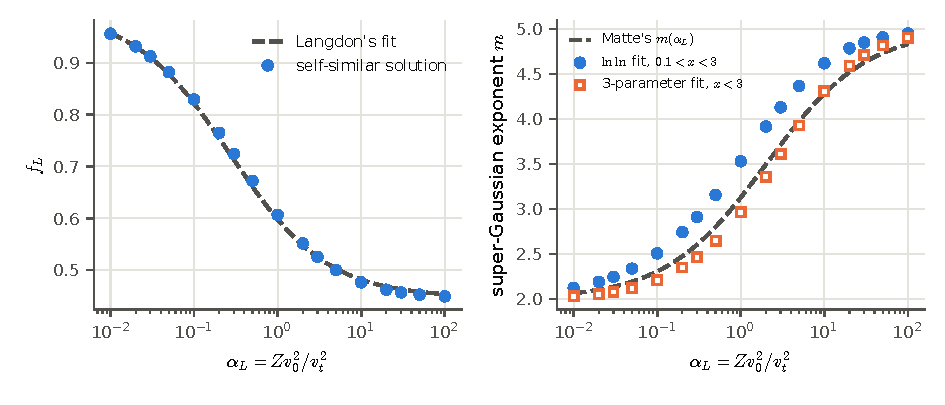
\includegraphics[width=\textwidth]{chapters/nl/fig_langdon.pdf}
\caption{Left: the absorption factor of the heated plasma against Langdon's
fit. Right: fitted super-Gaussian exponents against Matte's.}
\label{nl:fig:langdon}
\end{figure}

{\noindent}(2) \emph{The gas.} With $n_e=0$, no ions and the discretization of
the first scheme of Sec.~\ref{nl:sec:method}, the solver reproduces an independent
two-term solver to $7\times10^{-11}$. A
constant cross section in a DC field gives the Druyvesteyn distribution
\cite{nl:Druyvesteyn1940} to $1.2\times10^{-7}$ in $\ln F$, a field with $\omega\gg\nu$ and
elastic losses the Maxwellian of Margenau \cite{nl:Margenau1946}, with or without
e-e collisions. The e-e flux conserves energy to $1.4\times10^{-17}$, its drift on a fast
electron is Spitzer's Eq.~\eqref{nl:eq:spitzer} to $2\times10^{-5}$, and two mixed
Maxwellians relax to one. The Coulomb heating of a 3~eV Maxwellian is
$(e^2E^2/m\omega^2)\nu_TL$ to $9\times10^{-5}$, once the half cell next to $\epsilon=0$
is accounted for. In a DC field e-e collisions turn the Druyvesteyn
distribution, whose $(2/3)\langle\epsilon\rangle/T_{\rm slope}$ is 1.50 with $T_{\rm slope}$
fitted to $\ln F$ on $0.1\langle\epsilon\rangle<\epsilon<4\langle\epsilon\rangle$, into a
Maxwellian: the ratio is 1.0005 at $n_e/N=10^{-2}$.

\section{Where gas lasers sit}
\label{nl:sec:regime}

{\noindent}(1) Table~\ref{nl:tab:regime} evaluates Eq.~\eqref{nl:eq:thresholds} for the
fields of three lasers and for auxiliary sources heating the Ne fill, with
Maxwellian electrons, the losses of the LXCat sets, and the ions of Eq.~\eqref{nl:eq:sigc}.
Every beam-on row has $T_e=1.5$~eV, between the temperature of a Maxwellian power
balance at beam-on density, 1.08~eV, and that of the beam-sustained electrons of
Sec.~\ref{nl:sec:share} at
beam-on density, 1.88 (Ar fill) and 2.04~eV (Ne fill), and $n_e=2.72\times10^{21}$~m$^{-3}$. The
afterglow rows have 0.63~eV and $10^{20}$~m$^{-3}$. The ArF fill is
Electra's, Ar/F$_2$ $=0.997/0.003$ at 0.82~atm \cite{nl:Obenschain2020}. The CO$_2$ row
uses a CO$_2$:N$_2$:He $=1:1:8$ mixture at 1~atm, $T_e=1$~eV and $n_e=10^{19}$~m$^{-3}$
with the IST-Lisbon cross sections \cite{nl:LXCat}, and singly charged cations only ($Z_{\rm eff}=1$).
Langdon's and Silin's intensities are left out where $\nu_m>\omega$, where the
electrons do not quiver freely. Figure~\ref{nl:fig:regime} shows the thresholds against
frequency.

\begin{table}[h]
\centering
\caption{Thresholds of the three nonlinearities, Eq.~\eqref{nl:eq:thresholds}, in
W\,cm$^{-2}$. $u=\hbar\omega/eT_e$; $\nu_m/\omega$ with the Maxwellian
$\langle\nu_m\rangle$; $P_{\rm loss}$ in eV\,s$^{-1}$ per electron; Langdon at
$\alpha_L=0.1$ with $Z_{\rm eff}=1.15$ (1 for the CO$_2$ discharge); Langdon and Silin
left out where $\nu_m>\omega$.}
\label{nl:tab:regime}
\footnotesize
\setlength{\tabcolsep}{3.5pt}
\begin{tabular}{lcccccccc}
\toprule
field, gas & $T_e$ & $n_e$ (m$^{-3}$) & $u$ & $\nu_m/\omega$ & $P_{\rm loss}$ & $I_{\rm heat}$ & $I_L$ & $I_S$\\
\midrule
\tabinput{chapters/nl/tab_regime.tex}
\bottomrule
\end{tabular}
\end{table}

\begin{figure}[h]
\centering
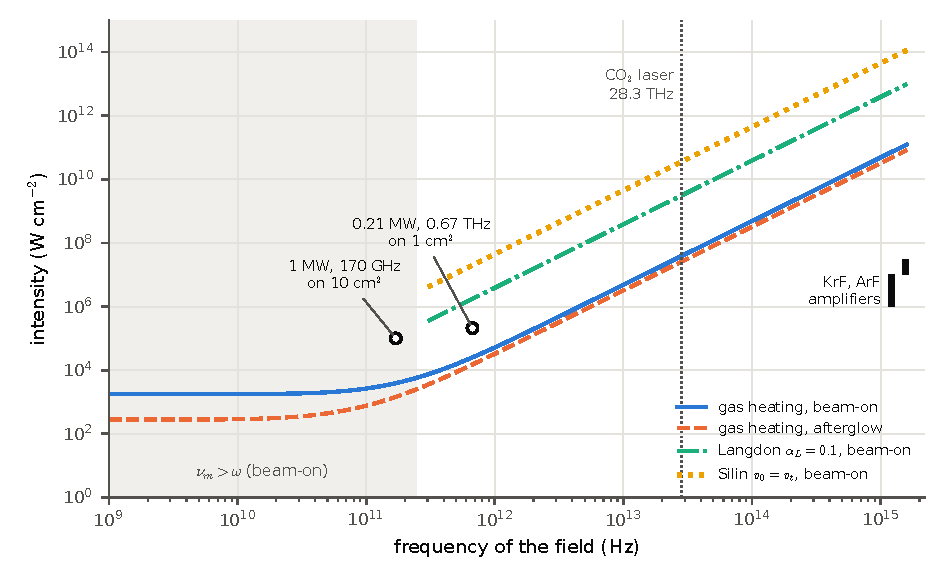
\includegraphics[width=0.9\textwidth]{chapters/nl/fig_regime.pdf}
\caption{The three thresholds against frequency in the Ne fill: gas heating
($I_{\rm heat}$) beam-on ($T_e=1.5$~eV, $n_e=2.72\times10^{21}$~m$^{-3}$) and in the
afterglow ($0.63$~eV, $10^{20}$~m$^{-3}$), Langdon at $\alpha_L=0.1$ and Silin,
both beam-on and drawn only where $\nu_m<\omega$. Bars: KrF amplifiers at 1 to 10 and
ArF amplifiers at 10 to 30~MW\,cm$^{-2}$ (Sec.~\ref{nl:sec:regime}); dotted line: the
CO$_2$-laser frequency 28.3~THz; circles: a 1~MW gyrotron at 170~GHz
\cite{nl:Sakamoto2007} and a 0.21~MW, 0.67~THz gyrotron \cite{nl:Glyavin2012},
each on an assumed spot.}
\label{nl:fig:regime}
\end{figure}

{\noindent}(2) \emph{The lasers' own fields.} An amplifier extracts at a few
saturation intensities. For KrF, $I_{\rm sat}=h\nu(A+Q)/\sigma$ is 1.0 and
1.2~MW\,cm$^{-2}$ in the two fills, with the cross section $2.6\times10^{-16}$~cm$^2$ and
radiative rate of Kannari et al.\ \cite{nl:Kannari1985} and the quench rates of a KrF
kinetic network at each fill's composition. Electra's ArF amplifier
saturates at 10~MW\,cm$^{-2}$ \cite{nl:Obenschain2020}. At 10~MW\,cm$^{-2}$ the KrF field is
$7.1\times10^3$ times below $I_{\rm heat}$ in the Ne fill and $1.5\times10^4$ times in the
Ar fill, and at 30~MW\,cm$^{-2}$ the ArF field is $5.8\times10^3$ times below it. These
margins depend on $T_e$ through the inelastic losses: for $T_e$ from 1.08 to 2.04~eV they
are $10^{3.2}$ to $10^{5.0}$. They also rest on the classical kernel at
$u=\hbar\omega/eT_e=3.3$ and 4.3, where it is not validated (the quantum absorption
on these atoms, from exact phase shifts of model potentials, is 10 to 28~\% below it at
$u=4.5$, for 300~K electrons at 28.3~THz, and its size for 5.0 and 6.4~eV photons
is not known). The excimer lasers' own fields are linear by every measure. The CO$_2$
laser's field supplies a tenth (0.10) of the energy budget of its discharge electrons at
100~MW\,cm$^{-2}$, and all of it at $I_{\rm heat}=9.6\times10^8$~W\,cm$^{-2}$. That is an
order-of-magnitude estimate. It assumes Maxwellian electrons at 1~eV, which at
$n_e/N=4\times10^{-7}$ nothing Maxwellizes, and discharge electrons present while the
pulse passes, which depends on the timing of the amplifier. Of the lasers examined it
is the one in which the lasing field can reach the gas nonlinearity. Lasing is known to perturb CO$_2$-laser
discharges, the optogalvanic effect, but through the vibrational kinetics of the laser levels
\cite{nl:Tachikawa1990}. No study was found of the field's IB heating of the
discharge electrons as an efficiency or stability term.

{\noindent}(3) \emph{Auxiliary fields.} Heating the Ne fill's electrons takes
$1.4\times10^3$~W\,cm$^{-2}$ at 170~GHz and $1.5\times10^4$~W\,cm$^{-2}$ at 0.67~THz
in the afterglow, and $5.2\times10^4$~W\,cm$^{-2}$ at 1~THz beam-on, within reach of
gyrotron beams \cite{nl:Sakamoto2007,nl:Glyavin2012}. Such a beam heats only its absorption length,
2.5~mm at 170~GHz and 2.6~cm at 0.67~THz in the afterglow and 1.1~mm at 1~THz beam-on.
Where $\nu_m<\omega/2$, Langdon's $\alpha_L=0.1$ needs 62 to 80 times $I_{\rm heat}$ in
the Ne fill beam-on, 33 to 51 times in its afterglow, and 37 and 54 times at the laser
frequencies of the Ar and ArF fills. Silin's $v_0=v_t$ needs a further
$Z_{\rm eff}/\alpha_L=11.5$ times. For $\omega\gg\nu_m$ the ratio is
Eq.~\eqref{nl:eq:ratio}, $\alpha_L/3Z_{\rm eff}\delta_{\rm eff}$, with
$\delta_{\rm eff}=4\times10^{-4}$ to $8\times10^{-4}$. In the excimer fills a field strong enough to matter is in the gas
nonlinearity, and only there. The CO$_2$ discharge, whose vibrational losses make
$\delta_{\rm eff}$ large, has Langdon's intensity only 2.5 times its $I_{\rm heat}$.

\section{Frequency as a lever on the distribution}
\label{nl:sec:share}

{\noindent}(1) Without e-e collisions a field above the collision frequency puts
more of its power into krypton than a DC field of the same absorbed power: at the
lowest power about twice as much in the Ne fill and up to 32 times as much in the Ar
fill, where the DC share is 1.3~\%. This section asks whether e-e collisions erase
that. The mechanism is item~(3) of Sec.~\ref{nl:sec:three}. A DC
field heats each electron in proportion to $1/\nu_m$, so in a gas whose $\nu_m$ rises
with energy it heats the slow electrons most and gives the Druyvesteyn-like
distribution, with a depleted tail. A field with $\omega\gg\nu_m$ heats in
proportion to $\nu_m$, which with elastic losses gives Margenau's Maxwellian
\cite{nl:Margenau1946}. Its tail reaches the 9.9~eV krypton levels. That the energy
dependence of $\nu_m$ decides how DC and microwave distributions differ is known for
discharges in general \cite{nl:Karoulina1988}, high-frequency argon distributions have
been computed from $\omega\ll\nu$ to $\omega\gg\nu$ \cite{nl:FerreiraLoureiro1983}, and e-e
collisions were added for argon discharges \cite{nl:Sa1992,nl:Wang1993}. What is new here is
the KrF laser gas and its formation chain. A scan repeats the comparison
at the absorbed powers per electron of DC fields of 2, 5 and 10~Td in the Ne fill and
3, 6 and 15~Td in the Ar fill, with e-e collisions
and ions at each electron density, and with the temporal-growth model of two-term
solvers: the electrons grow or decay with the shape of $F$. Item~(3) repeats it with
electrons born from the beam. The scan treats the field as given inside the gas. At beam-on density the
plasma frequency is 0.47~THz, so a 0.3~THz wave would not enter the gas there. How a
field reaches the gas is a separate question of coupling.

{\noindent}(2) Table~\ref{nl:tab:share} and Fig.~\ref{nl:fig:share} give the result.
Electron--electron collisions raise krypton's share in the DC field, from 27.5 to
80.1~\% at the power of 2~Td in the Ne fill, as $n_e$ rises from 0 to the beam-on
density $2.72\times10^{21}$~m$^{-3}$. The 28.3~THz field goes from 54.2 to
84.5~\%. Collisions bring both towards the Maxwellian, which is where the high
frequency was already taking the distribution. At the 9.9~eV krypton threshold,
relative to a Maxwellian of the same mean energy, the DC distribution holds 0.556
of the population and the 28.3~THz one 0.742 without e-e collisions, and 0.900 and
0.969 at beam-on density. Over the 30 series of the scan that
ratio moves towards 1 between $n_e=0$ and beam-on density in 29, and stays at 0.94 in
the Ar fill at 6~Td and 3~THz. Where the advantage is large, at 2~Td in the Ne fill
and at 3 and 6~Td in the Ar fill, the 28.3~THz ratio rises and the DC one rises more.
The advantage of the frequency therefore falls from
$\times1.97$ to $\times1.055$. Normalized by its value without e-e collisions,
the advantage falls along nearly one curve of $\alpha_g$ for the three power levels
in Fig.~\ref{nl:fig:share}. It halves at $\alpha_g=0.41$, 0.46 and 0.55, found by root
finding in $n_e$ between the scan's grid points. At beam-on
density $\alpha_g$ is 0.023 to 0.14 for these three levels and the frequency is
worth 2.0 to 5.5~\%. In the Ne fill at the highest power, 10~Td, the high frequency
is worse than DC. The fatter tail excites neon itself (its share rises from 1.9 to
7.2~\%), and krypton's share falls by 3.0 points. In the Ar fill at 15~Td the high
frequency is still 2.9 points better without e-e collisions, and 0.6 points worse at
beam-on density.

\begin{table}[h]
\centering
\caption{Krypton's share of the absorbed power (\%) and the formation efficiency
$\eta_{\rm form}$ of Sec.~\ref{nl:sec:wallplug}, DC against 28.3~THz at the same absorbed
power per electron (that of a DC field of the given $E/N$ without e-e
collisions). $\alpha_g$ of the DC point, Eq.~\eqref{nl:eq:alphag}.}
\label{nl:tab:share}
\setlength{\tabcolsep}{5pt}
\begin{tabular}{lccccccc}
\toprule
fill, power & $n_e$ (m$^{-3}$) & $\alpha_g$ & Kr, DC & Kr, 28.3~THz & ratio & $\eta_{\rm form}$, DC & $\eta_{\rm form}$, 28.3~THz\\
\midrule
\tabinput{chapters/nl/tab_share.tex}
\bottomrule
\end{tabular}
\end{table}

\begin{figure}[h]
\centering
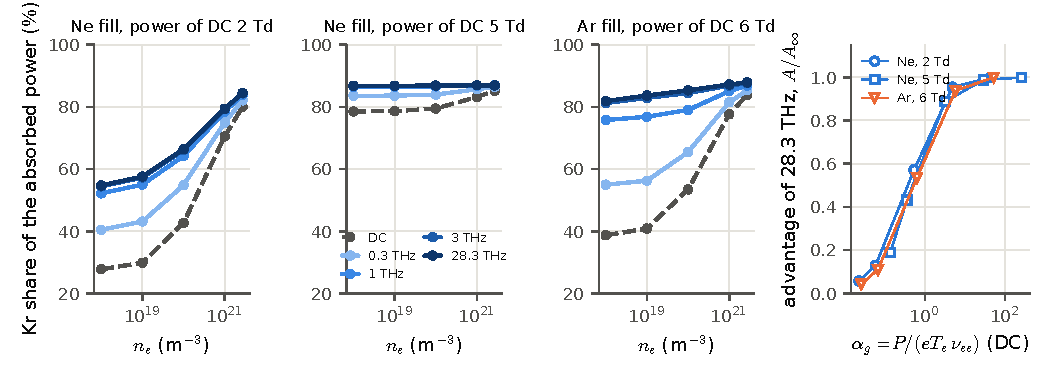
\includegraphics[width=\textwidth]{chapters/nl/fig_share.pdf}
\caption{Krypton's share of the absorbed power against $n_e$, DC (dashed) and
0.3, 1, 3 and 28.3~THz, and (right) the advantage of 28.3~THz over DC,
$A=$ ratio $-1$, normalized by its value without e-e collisions, against
$\alpha_g$. Every point drawn has $P_{\rm field}>1.5\,|P_{\rm growth}|$. The Ar fill at
3~Td is not shown: from $10^{19}$~m$^{-3}$ up its points at 1 to 28.3~THz fall below that.}
\label{nl:fig:share}
\end{figure}

{\noindent}(3) \emph{Beam-sustained electrons.} \label{nl:sec:source}The growth model lets new electrons
appear with the shape of $F$, and at the lowest power its term carries up to 0.66 of
the absorbed power at the points kept, those with $P_{\rm field}>1.5\,|P_{\rm growth}|$.
In an e-beam pumped gas the electrons are born from the beam and lost by attachment and
by recombination. A second scan therefore repeats the comparison at the
absorbed powers of Table~\ref{nl:tab:share} with electrons injected with the beam's
sub-excitation spectrum (item~(6) of Sec.~\ref{nl:sec:kinetic}) and lost by attachment and
by dissociative recombination on $1.075\,n_e$ cations, taken as Kr$_2^+$ with the rate
$2.24\times10^{-7}\,T_e^{-1/2}$~cm$^3$\,s$^{-1}$, built on the dissociative recombination
rates of Kannari et al.\ \cite{nl:Kannari1985}. The loss has a cross
section $\propto1/\epsilon$, which gives that rate for a Maxwellian, so it takes the slow
electrons first. At beam-on density recombination removes electrons 3.1 (Ne fill) and 3.9 (Ar
fill) times faster than attachment, and with the DC field the beam's own injected power
is then 2.4 to 8.3 times the field's, except at 5~Td in the Ne fill (0.425).
Table~\ref{nl:tab:source}
gives the field's marginal share to krypton at fixed $n_e$, the change of krypton's power per unit field power. It
charges the field with the change of the beam's injected power, which follows the
attachment and recombination of the heated distribution. Crediting the beam with its own
partition at that power gives the second ratio of the table. Neither ratio holds the
beam current fixed. Holding it means finding the electron density at which the beam's
injected power per unit volume, and so its current, keeps its value without the field,
and the field's absorbed power per unit volume keeps its value at fixed $n_e$. At beam-on
density the advantage at a fixed beam current is within 0.01 of the second ratio. At
$10^{18}$~m$^{-3}$ the field changes the density by a factor $x=0.36$ to 1.44, and the
advantage at a fixed current, $\times1.23$ to $\times13.5$, exceeds both ratios. That
excess is the field's power per electron, which a fixed absorbed power per unit volume
changes by $1/x$: with the field's amplitude held instead, the advantage at a fixed
current is the fixed-$n_e$ one within 1~\%. The ranges below
leave out the points where, with the DC field, the beam injects more power than the
field absorbs. At $10^{18}$~m$^{-3}$ and fixed $n_e$ the frequency raises krypton's share $\times2.06$
in the Ne fill at 2~Td and $\times2.40$ in the Ar fill at 6~Td, against $\times1.97$ and
$\times2.12$ with the growth model, and $\times11.7$ in the Ar fill at 3~Td, against
$\times27$ with the growth model at the same density. At beam-on density, where only the
Ne fill at 5~Td is kept, the advantage is $\times1.05$ to $\times1.07$, against $\times1.020$
with the growth model at the same power, and the field sends 75 to 85~\% of its power to
krypton, against 85 to 87~\%. Where the beam outweighs the field the advantage is
$\times1.10$ to $\times1.14$ at a fixed beam current and up to $\times1.27$ at fixed
$n_e$. Counted per change of the total input power, the beam's and
the field's together, it is $\times1.03$ to $\times1.07$ at every beam-on point. Where the frequency's
advantage is large it collapses in both models, and its size
at beam-on density depends on how the electrons are created and lost and on how the
field's share is counted. Without a field, the e-e collisions at beam-on density send
38.9~\% of the injected sub-excitation energy into krypton in the Ne fill and 44.7~\% in
the Ar fill, against 0.0~\% at $10^{18}$~m$^{-3}$, and recombination takes 34 to 35~\%
of it. That is an e-beam effect independent of any field. A loss that takes electrons
of every energy alike at the
same Maxwellian rate gives 28.5 and 34.2~\%, with recombination taking 47 to 49~\%, and
nearly the same advantage at 5~Td in the Ne fill, $\times1.06$ to $\times1.07$. The
beam's own numbers depend on the form of the recombination, and the frequency's
advantage much less: at beam-on density each of its four counts moves by at most 0.013
at 5~Td in the Ne fill and 0.044 where the beam outweighs the field.

The beam-on density used throughout, $2.72\times10^{21}$~m$^{-3}$, is the peak that a
full kinetic model of the Ne-fill laser gives under 0.6~MW\,cm$^{-3}$ of beam. This note's model
holds it only with $1.6\times10^{30}$ ion pairs per m$^3$ and second, 7.9~MW\,cm$^{-3}$ at
the chain's 30.4~eV per pair, which is 13 times that beam, or 2.5~MW\,cm$^{-3}$ without
recombination. Taking every cation as Kr$_2^+$ overstates the recombination of both
fills: Kr$^+$ forms Kr$_2^+$ by three-body association in 33~ns in the Ne fill and 17~ns
in the Ar fill at that model's $2.5\times10^{-31}$~cm$^6$\,s$^{-1}$, while Kr$_2^+$
recombines in 2~ns at beam-on density. That model by default extrapolates its attachment
below the floor of its measured tables, and with the measured tables its peak falls to 0.56
of that density. With its beam this note's model holds $5.2\times10^{20}$~m$^{-3}$ in the
Ne fill, and there the advantage is $\times1.157$ to $\times1.355$ at 2~Td and
$\times1.051$ to $\times1.107$ at 5~Td in the four counts. That density is a lower bound.
Besides overstating recombination, the model injects one electron per ion pair, where
the chain of Sec.~\ref{nl:sec:wallplug} frees 1.56 through the Penning ionization of krypton
by Ne$^*$, and with those it holds $6.2\times10^{20}$ to $7.1\times10^{20}$~m$^{-3}$ at 36.6
to 30.4~eV per pair. Without recombination the advantage at beam-on density is $\times1.01$ to
$\times1.18$. The density of the beam-pumped gas, and with it what is left of the
frequency's advantage, is uncertain by a factor of about five.

\begin{table}[h]
\centering
\caption{The beam-sustained model: electrons injected with the
beam's sub-excitation spectrum and lost by attachment and recombination, at the absorbed
powers of Table~\ref{nl:tab:share}. Krypton's marginal share
$(P_{\rm Kr}-P_{\rm Kr,beam})/P_{\rm field}$ (\%) at fixed $n_e$, the ratio of 28.3~THz
over DC with it, with the beam credited with its own partition at its injected power
(fixed beam), and at a fixed beam current (see the text), and the formation efficiency of the
field's marginal power at fixed $n_e$.
$P_{\rm beam}/P_{\rm field}$ is the beam's injected power over the field's, with the DC
field; in the rows marked $\dagger$ the beam outweighs the field.}
\label{nl:tab:source}
\footnotesize
\setlength{\tabcolsep}{3.5pt}
\begin{tabular}{lccccccccc}
\toprule
fill, power & $n_e$ (m$^{-3}$) & $P_{\rm beam}/P_{\rm field}$ & Kr, DC & \shortstack{Kr,\\28.3~THz} & \shortstack{ratio,\\fixed $n_e$} & \shortstack{ratio,\\fixed beam} & \shortstack{ratio, fixed\\current} & $\eta_{\rm form}$, DC & \shortstack{$\eta_{\rm form}$,\\28.3~THz}\\
\midrule
\tabinput{chapters/nl/tab_source.tex}
\bottomrule
\end{tabular}
\end{table}

\section{The self-sustained discharge}
\label{nl:sec:selfsus}

{\noindent}(1) A discharge-pumped laser needs ionization to balance attachment.
At $\nu_{\rm net}=0$ the growth model drops out, which makes this the cleanest
comparison of field shapes. A third scan finds the rms field of
self-sustainment from DC to $\omega/N=10^{-11}$~m$^3$\,s$^{-1}$ (78~THz in the Ne
fill) for $n_e/N=0$ to $10^{-4}$ (Table~\ref{nl:tab:selfsus},
Fig.~\ref{nl:fig:selfsus}).

\begin{table}[h]
\centering
\caption{The self-sustained discharge: DC, the frequency of the largest krypton
share, and $\omega/N=10^{-11}$~m$^3$\,s$^{-1}$. $P$ in eV\,s$^{-1}$ per electron;
Kr and buffer shares in \%.}
\label{nl:tab:selfsus}
\begin{tabular}{lccccccccc}
\toprule
fill & $n_e/N$ & $\omega/N$ (m$^3$\,s$^{-1}$) & $E/N$ (Td) & $\langle\epsilon\rangle$ (eV) & $P$ & Kr & buffer & $\eta_{\rm form}$\\
\midrule
\tabinput{chapters/nl/tab_selfsus.tex}
\bottomrule
\end{tabular}
\end{table}

\begin{figure}[h]
\centering
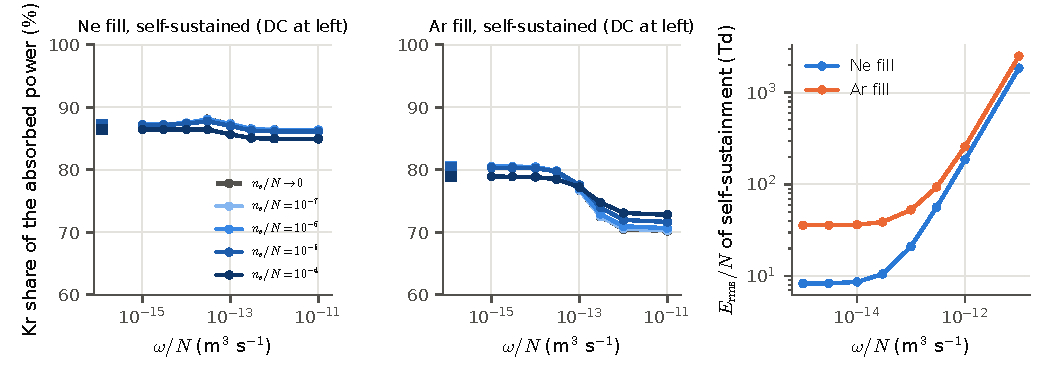
\includegraphics[width=\textwidth]{chapters/nl/fig_selfsustained.pdf}
\caption{Self-sustained discharges against $\omega/N$: krypton's share in the two
fills (DC at the left, squares) and the rms $E/N$ of self-sustainment.}
\label{nl:fig:selfsus}
\end{figure}

{\noindent}(2) In the Ne fill the discharge sustains itself at 8.33~Td DC with
87.2~\% of its power in krypton. On the grid of the scan the share peaks at
88.1~\% at $\omega/N=3\times10^{-14}$~m$^3$\,s$^{-1}$, a third of the Maxwellian
mean $\langle\nu_m\rangle/N=9.2\times10^{-14}$~m$^3$\,s$^{-1}$ at the discharge's mean
energy: the optimum sits where $\omega$ and $\nu_m$ are of the same order. A Canon
patent on microwave-excited excimer lasers states that at 35~GHz ``the plasma
excitation efficiency based on identical electric power is highest'' at the
pressure, 160~Torr, at which the collision frequency of electrons with neon, the main
body of the Kr/Ne/F$_2$ gas, equals the microwave frequency \cite{nl:Canon}. The optimum exists but is
worth 0.9 points. Far above the collision frequency the share
falls to 86.4~\%, the fatter tail exciting neon. In the Ar fill the discharge needs
35.9~Td DC and gives 80.5~\% to krypton, falling to 70.2~\% at high frequency as
argon's 11.5~eV levels take the tail. The formation efficiency moves less, from
0.351 to 0.337, because argon's excitation partly reaches KrF$^*$. Raising $n_e/N$ to
$10^{-4}$ changes these shares by at most 2.6 points.

\section{What field pumping buys}
\label{nl:sec:wallplug}

{\noindent}(1) A formation efficiency turns a
power partition into KrF$^*$ per absorbed energy,
\begin{equation}
\eta_{\rm form}=\sum_cf_c\,\frac{h\nu}{u_c}\,b_c,
\label{nl:eq:etaform}
\end{equation}
with $f_c$ the shares, $u_c$ the energy per event (Kr excitation 10.5~eV, ionization
14.0, Ne 17.5, Ar 12.5), $h\nu=4.997$~eV, and $b_c$ the branchings of a KrF kinetic
network for each fill (Kr$^*$ harpoon 0.87 and 0.81, ion channel 0.68). The same
accounting gives e-beam pumping of the Ne fill 0.175, from 30.4~eV per ion pair and 0.7
excitations per ion with this fill's Ne$^*\to$Kr$^+$ branching 0.80. That accounting
gives the beam's sub-excitation electrons
nothing. At beam-on density their e-e collisions put 0.159 of their energy into
KrF$^*$ (Sec.~\ref{nl:sec:share}, where recombination takes about a third of it), and one
such electron of 4.506~eV per 30.4~eV ion pair adds 0.024: the like-for-like e-beam
figure there is 0.198. A full kinetic model of the Ne-fill laser, whose Spencer--Fano
partition has 36.6~eV per ion pair where the chain counts 30.4, also forms 0.194 of its
deposited energy into KrF$^*$ at the photon energy, its 1.42 KrF$^*$ per ion pair
against 1.21 here making up for the larger energy per pair. The chain has no e-beam
accounting for the Ar fill.

{\noindent}(2) Field pumping of the beam-ionized gas at beam-on density has
$\eta_{\rm form}=0.327$ to 0.365 where the field dominates in the growth model
(Table~\ref{nl:tab:share}), 0.327 to 0.349 in the Ne fill, and 0.30 to 0.34 for the field's
marginal power with beam-sustained electrons in the Ne fill at 5~Td, in both attributions
and at a fixed beam current (Table~\ref{nl:tab:source} gives the fixed-$n_e$ values). The self-sustained discharge
gives 0.337 to 0.354. In the Ne fill at beam-on density, where the field's power exceeds
the beam's own, field pumping thus forms 1.5 to 1.8 times as much as the e-beam's 0.198,
and the frequency moves it by $-4$ to $+6$~\%. At 2~Td, where the beam outweighs the
field, the field's marginal power gives 0.30 to 0.33 at a fixed beam current, 1.5 to 1.7
times the e-beam's, and the frequency raises it by 9~\% (from 0.265 and by 15~\% counted
at fixed $n_e$). This is the rationale of the e-beam-controlled discharge, demonstrated for
KrF by Mangano and Jacob \cite{nl:ManganoJacob1975}, and a KrF laser pumped by the
discharge that an IR laser beam drives in the gas has also been modelled
\cite{nl:Igoshin1993}. Field pumping beats beam pumping at the wall plug when
$\eta_{\rm src}\,\eta_{\rm form,f}>\eta_{\rm beam}\,\eta_{\rm form,b}$, i.e.\ when the
source efficiency exceeds 0.57 to 0.65 of the efficiency with which the pulsed power
puts energy into the gas through the foil. The chain's branchings do not depend on
$n_e$. At beam-on density the stepwise ionization $e+{\rm Kr}^*\to{\rm Kr}^++2e$ runs at
0.39 to 1.63 of the harpoon rate in the Ne fill, rising with the power (Kannari's rate
at the scan's $T_e$ \cite{nl:Kannari1985}). It moves Kr$^*$ from the harpoon channel (0.87) to
the ion channel (0.68), which lowers the KrF$^*$ yield of a Kr$^*$ by 4.8 to 11.8~\%,
and so lowers field pumping, which goes mostly through Kr$^*$, more than beam pumping,
which goes through ions. In a full kinetic model of microwave co-pumping, the sign
of the laser energy that a co-pumping field gains rests on that one rate, and the
electron quench of KrF$^*$ is a candidate second such rate. The first
depends on $T_e$, and the second may. Those rates, not the frequency,
decide whether field pumping pays.

\section{At the target}
\label{nl:sec:ife}

{\noindent}(1) In a direct-drive corona Langdon's $\alpha_L\propto
Z_{\rm eff}I\lambda^2/T_e$ favours short wavelengths. Obenschain et al.\ computed
the quarter-critical temperature and intensity of a 2.6~mm CH sphere driven at 351,
248 and 193~nm (their Table~1, averaged over 2 to 3~ns) \cite{nl:Obenschain2020}. With
fully ionized CH, $Z_{\rm eff}=37/7$, Table~\ref{nl:tab:ife} gives $\alpha_L$ and four
estimates of $f_L$: Langdon's fit, Matte's super-Gaussian, Eq.~\eqref{nl:eq:selfsim}
with a constant logarithm, and Eq.~\eqref{nl:eq:selfsim} with the quantum logarithm
$L=\ln(2mv^2/\hbar\omega)$ of one electron in both the operator and the absorption.
The last is the kinetic counterpart of the improved factor of Turnbull et al.\
\cite{nl:Turnbull2024}, which weights a super-Gaussian with a velocity-dependent Gaunt
factor and which Sherlock et al.\ treat more thoroughly \cite{nl:Sherlock2024}. The e-e
logarithm is the NRL formulary's electron--electron value at $n_c/4$ \cite{nl:NRL},
$\lnL_{ee}=7.7$, 7.2 and 6.8 at 351, 248 and 193~nm. All of it is for a homogeneous
plasma at the time-averaged conditions, with the self-similar distribution at fixed
$\alpha_L$. Nonlocal transport near $n_c/4$ and the structure of the beam are left out.

\begin{table}[h]
\centering
\caption{The Langdon factor at the quarter-critical conditions of
\cite{nl:Obenschain2020}, Table~1. $I$ in $10^{14}$~W\,cm$^{-2}$.}
\label{nl:tab:ife}
\begin{tabular}{cccccccc}
\toprule
$\lambda$ (nm) & $T_e$ (keV) & $I$ & $\alpha_L$ & fit & Matte & kinetic, const.\ $L$ & kinetic, $L(v)$\\
\midrule
\tabinput{chapters/nl/tab_ife.tex}
\bottomrule
\end{tabular}
\end{table}

{\noindent}(2) The kinetic solution with a constant logarithm reproduces the fit
within 0.22~\%. The velocity-dependent logarithm cuts the penalty $1-f_L$ to 0.64,
0.58 and 0.52 of the fit's, in line with the finding of Turnbull et al.\ that the
velocity dependence of the Gaunt factor ``somewhat mitigates the Langdon effect''
\cite{nl:Turnbull2024}. The nonlinear factor alone makes the local absorption rate at
quarter critical higher than at 351~nm by $\times1.031$ (KrF) and $\times1.052$ (ArF)
with Langdon's fit, and by $\times1.023$ and $\times1.038$ with the velocity-dependent
logarithm. The linear coefficient itself, proportional to
$n_cT_e^{-3/2}\propto\lambda^{-2}T_e^{-3/2}$ at quarter critical apart from the
logarithm, is $\times2.53$ and $\times5.20$ that of 351~nm at the same conditions. The
nonlinearity thus adds a few percent to a much larger linear advantage of the excimer
drivers. The Langdon effect has been reviewed for laser plasmas \cite{nl:Shaffer2025},
computed for short KrF pulses on selenium \cite{nl:Pulsifer1994}, and quantified against
$I\lambda^2$ for the plasmas of extreme-ultraviolet sources, where it lowers the
absorption by 10 to 20~\% \cite{nl:GonzalezSheil2025}. No published quantification of
this wavelength dependence for excimer drivers was found, though not every candidate
could be read in full. The bandwidths of Obenschain et al.'s
Table~1, 1, 3 and 10~THz, give speckle lifetimes $1/\Delta\nu$ of 1.0, 0.33 and
0.10~ps, shorter than the e-e time $1/\nu_{ee}$ at quarter critical (4.8, 2.0 and
1.0~ps). Whether that changes the Langdon factor of a speckled beam is open. Shaffer
et al.\ found that the Langdon operator predicts the heating well in the simple cases
they considered. For a two-colour field it gave slightly less heating than their full
calculation, as it did without bandwidth, and a weaker, phase-shifted beat modulation,
which they attribute to its steady-state assumption breaking down for broadband light
\cite{nl:Shaffer2023}. The scattering of electrons on speckles changes both absorption
and transport \cite{nl:SherlockMichel2022}.

\section{Verdict and next steps}
\label{nl:sec:verdict}

{\noindent}(1) The nonlinear behavior of IB does not by itself improve a gas
laser. The lasing field of an excimer laser stays more than $10^3$ times below it. An
auxiliary field reaches only the gas nonlinearity, whose effect on the distribution the
electron--electron collisions of a pumped laser largely supply: what is left of the
frequency's advantage at the beam-on density is 2 to 7~\% where the field's power
exceeds the beam's own and 10 to 14~\% at a fixed beam current where the beam's is larger
(1 to 18~\% without recombination), and up to $\times1.24$ at a fixed beam current
($\times1.355$ at fixed $n_e$) at the five times lower density that this note's electron
source and losses give with the beam of the full kinetic model. At the target the
nonlinearity
is worth a few percent of absorption rate to KrF and ArF. The ranked next steps,
cheapest decisive first:
\begin{enumerate}
\item \emph{The instrument.} Fit THz transmission of the laser gas with this
  solver, which carries the field, the ions and e-e, to read $n_e$ and $T_e$, and
  use a THz $T_e$ jump to measure $e+{\rm Kr}^*\to{\rm Kr}^++2e$ and the electron
  quench of KrF$^*$. The first decides the sign of the
  co-pump in a full kinetic model, the second is the candidate for a second such rate.
\item \emph{Field co-pumping at beam-class power}, frequency-blind: run a full kinetic
  model of the laser in pairs, with and without the field, with this solver's partition
  (Tables~\ref{nl:tab:share} and~\ref{nl:tab:source}) and the uncertain rates bracketed, with the
  electron collisions on Kr$^*$ and KrF$^*$ that the formation chain leaves out.
\item \emph{The e-beam's own sub-excitation electrons.} Item~(3) of
  Sec.~\ref{nl:sec:share} sends 39~\% of their energy to krypton at beam-on density
  through e-e collisions in the Ne fill (45~\% in the Ar fill), which raises the
  e-beam's formation efficiency from 0.175 to 0.198. Check whether the energy
  accounting of full kinetic models of the laser carries it.
\item \emph{The electron source.} The residual advantage at beam-on density depends
  on how the electrons are created and lost and on how the field's share is counted
  (1 to 28~\%), and on the density itself, which this note's electron source and losses
  and a full kinetic model put about five times apart. Held at a fixed beam current in the steady state it is within 0.01
  of the fixed-beam ratio (Sec.~\ref{nl:sec:source}). A run in time with the beam's source,
  attachment, recombination on the fill's own mix of cations and the field together
  would settle it.
\item \emph{CO$_2$ lasers.} Of the lasers examined, the one whose own field heats
  its electrons at the 10~\% level, by an order-of-magnitude estimate. Compute it with
  the discharge's own distribution and timing, and its effect on the vibrational
  partition and on discharge stability for high-intensity amplifiers.
\item \emph{The target.} Use the velocity-dependent Langdon factor in the
  wavelength studies of excimer drivers, and test whether THz bandwidth and speckle
  change it.
\end{enumerate}

\chapterappendix
\section{The electron--electron operator in energy}
\label{nl:app:ee}

{\noindent}(1) The isotropic Rosenbluth operator for electrons of distribution
$f(v)$, $\int4\pi v^2f\,\dd v=n_e$, is \cite{nl:Rosenbluth1957}
\begin{equation}
\frac{\partial f}{\partial t}=\frac{4\pi\Gamma}{v^2}\frac{\partial}{\partial v}
\Big[f\,I_2+\frac{I_4+v^3J_1}{3v}\frac{\partial f}{\partial v}\Big],\qquad
\Gamma=\frac{e^4\lnL}{4\pi\epsilon_0^2m^2},
\end{equation}
with $I_2=\int_0^vu^2f$, $I_4=\int_0^vu^4f$, $J_1=\int_v^\infty uf$. For a
Maxwellian $J_1=v_t^2f$ and $I_4=3v_t^2I_2-v^3v_t^2f$, so the bracket vanishes.

{\noindent}(2) Write $h(v,w)=\min(v,w)^3/3$. Since $\partial_wh=w^2$ for $w<v$
and 0 above, $-\int f'(w)h\,\dd w=I_2$. And $(I_4+v^3J_1)/3v=\int f(w)(w/v)h\,\dd w$.
The bracket is therefore
\begin{equation}
\int_0^\infty w\,h(v,w)\Big[f(w)\frac{f'(v)}{v}-f(v)\frac{f'(w)}{w}\Big]\dd w,
\end{equation}
so $v$ times the bracket has the symmetric weight $v\,w\,h$ and an antisymmetric
bracket, which is the Landau form. In energy, $f'(v)/v=(m/e)\,\partial_\epsilon f$ and
$w\,\dd w=(e/m)\dd\epsilon'$, and with $f=n_e(2\pi)^{-1}(m/2e)^{3/2}F$ the upward
number flux per electron becomes Eq.~\eqref{nl:eq:ee-landau}.

{\noindent}(3) Integrating by parts in $\epsilon'$,
$\int\min^{3/2}[F(\epsilon')F'-FF'(\epsilon')]\dd\epsilon'=F'(A_2+\epsilon^{3/2}A_3)+\tfrac32A_1F$,
which is half the bracket of Hagelaar and Pitchford, so their $a$ \cite{nl:HP2005}
equals $(2\Gamma/3)(m/2e)^{3/2}=e^2\gamma\lnL/24\pi\epsilon_0^2$, as written in
Eq.~\eqref{nl:eq:ee-landau}.

\section{The checks}
\label{nl:app:checks}

\noindent A check script computes every result, or reloads it from the stored output
of the scan that made it and recomputes a sample of that output, and tests it. It
recomputes the computed numbers of the prose to their printed digits, each inside a
sentence that occurs once in the text, compares the inputs the text states with the
code that uses them, and tests the worded claims against the data. It re-derives the
displayed formulas numerically and requires them in the text as printed. The numbers
quoted from sources were checked against the sources by hand. Table~\ref{nl:tab:checks}
counts the checks by the section they support.

{\small
\begin{longtable}{L{6.4cm}ccc}
\caption{The checks of these notes, by the section whose statements, equations, tables and figures they support: all checks, the computed numbers of the prose recomputed to their printed digits, and the worded claims tested against the data.}\label{nl:tab:checks}\\
\toprule
supports & checks & printed numbers & claims\\
\midrule
\endfirsthead
\toprule
supports & checks & printed numbers & claims\\
\midrule
\endhead
\bottomrule
\endfoot
Sec.~\ref*{nl:sec:answer} & 58 & 40 & 16\\
Sec.~\ref*{nl:sec:three} & 18 & 8 & 1\\
Sec.~\ref*{nl:sec:kinetic} & 46 & 12 & 5\\
Sec.~\ref*{nl:sec:checks} & 20 & 8 & 3\\
Sec.~\ref*{nl:sec:regime} & 45 & 20 & 19\\
Sec.~\ref*{nl:sec:share} & 150 & 95 & 30\\
Sec.~\ref*{nl:sec:selfsus} & 23 & 14 & 5\\
Sec.~\ref*{nl:sec:wallplug} & 61 & 47 & 4\\
Sec.~\ref*{nl:sec:ife} & 29 & 18 & 4\\
Sec.~\ref*{nl:sec:verdict} & 17 & 14 & 3\\
Appendix~\ref*{nl:app:ee} & 1 &  & \\
Appendix~\ref*{nl:app:checks} & 2 &  & \\
the references and the text as a whole & 65 &  & \\
\midrule
Total & 535 & 276 & 90\\
\end{longtable}
}


\raggedright
\begin{thebibliography}{99}
\bibitem{nl:Langdon1980} A. B. Langdon, Nonlinear inverse bremsstrahlung and
heated-electron distributions, Phys. Rev. Lett. \textbf{44}, 575 (1980),
doi:10.1103/PhysRevLett.44.575.
\bibitem{nl:Matte1988} J. P. Matte, M. Lamoureux, C. M\"oller, R. Y. Yin,
J. Delettrez, J. Virmont and T. W. Johnston, Non-Maxwellian electron
distributions and continuum X-ray emission in inverse bremsstrahlung heated
plasmas, Plasma Phys. Control. Fusion \textbf{30}, 1665 (1988),
doi:10.1088/0741-3335/30/12/004.
\bibitem{nl:Turnbull2023} D. Turnbull et al., Inverse bremsstrahlung absorption,
Phys. Rev. Lett. \textbf{130}, 145103 (2023), doi:10.1103/PhysRevLett.130.145103.
\bibitem{nl:Turnbull2024} D. Turnbull et al., Reconciling calculations and
measurements of inverse bremsstrahlung absorption, Phys. Plasmas \textbf{31},
063304 (2024), doi:10.1063/5.0203446.
\bibitem{nl:Milder2021} A. L. Milder et al., Measurements of non-Maxwellian electron
distribution functions and their effect on laser heating, Phys. Rev. Lett.
\textbf{127}, 015001 (2021), doi:10.1103/PhysRevLett.127.015001.
\bibitem{nl:QBE} C. K. Watson et al., Unified microscopic foundations of the quantum
Boltzmann equation, Fluct. Noise Lett. \textbf{25}, 2640002 (2026),
doi:10.1142/S021947752640002X.
\bibitem{nl:Atzeni2004} S. Atzeni and J. Meyer-ter-Vehn, \emph{The Physics of Inertial
Fusion} (Oxford University Press, Oxford, 2004),
doi:10.1093/acprof:oso/9780198562641.001.0001.
\bibitem{nl:Glyavin2012} M. Yu. Glyavin, A. G. Luchinin, G. S. Nusinovich, J. Rodgers,
D. G. Kashyn, C. A. Romero-Talamas and R. Pu, A 670 GHz gyrotron with record power and
efficiency, Appl. Phys. Lett. \textbf{101}, 153503 (2012), doi:10.1063/1.4757290.
\bibitem{nl:HP2005} G. J. M. Hagelaar and L. C. Pitchford, Solving the Boltzmann
equation to obtain electron transport coefficients and rate coefficients for fluid
models, Plasma Sources Sci. Technol. \textbf{14}, 722 (2005),
doi:10.1088/0963-0252/14/4/011.
\bibitem{nl:Rosenbluth1957} M. N. Rosenbluth, W. M. MacDonald and D. L. Judd,
Fokker--Planck equation for an inverse-square force, Phys. Rev. \textbf{107}, 1
(1957), doi:10.1103/PhysRev.107.1.
\bibitem{nl:WalkerNi2011} H. F. Walker and P. Ni, Anderson acceleration for
fixed-point iterations, SIAM J. Numer. Anal. \textbf{49}, 1715 (2011),
doi:10.1137/10078356X.
\bibitem{nl:Druyvesteyn1940} M. J. Druyvesteyn and F. M. Penning, The mechanism of
electrical discharges in gases of low pressure, Rev. Mod. Phys. \textbf{12}, 87
(1940), doi:10.1103/RevModPhys.12.87.
\bibitem{nl:Margenau1946} H. Margenau, Conduction and dispersion of ionized gases at
high frequencies, Phys. Rev. \textbf{69}, 508 (1946), doi:10.1103/PhysRev.69.508.
\bibitem{nl:Obenschain2020} S. P. Obenschain et al., Direct drive with the argon
fluoride laser as a path to high fusion gain with sub-megajoule laser energy,
Phil. Trans. R. Soc. A \textbf{378}, 20200031 (2020), doi:10.1098/rsta.2020.0031.
\bibitem{nl:Canon} T. Ohmi, N. Tanaka and M. Hirayama (Canon Inc.), Excimer laser
oscillation apparatus and method, excimer laser exposure apparatus, and laser tube,
US Patent 6,331,994 B1 (published 2001-12-18).
\bibitem{nl:Silin1965} V. P. Silin, Nonlinear high-frequency plasma conductivity,
Sov. Phys. JETP \textbf{20}, 1510 (1965) [Zh. Eksp. Teor. Fiz. \textbf{47}, 2254
(1964)], record at \url{http://www.jetp.ras.ru/cgi-bin/e/index/e/20/6/p1510?a=list}.
\bibitem{nl:Karoulina1988} E. V. Karoulina and Yu. A. Lebedev, The influence of the
electron transport cross sectional shape on electron energy distribution functions in
DC and microwave plasmas, J. Phys. D \textbf{21}, 411 (1988),
doi:10.1088/0022-3727/21/3/006.
\bibitem{nl:FerreiraLoureiro1983} C. M. Ferreira and J. Loureiro, Electron energy
distributions and excitation rates in high-frequency argon discharges, J. Phys. D
\textbf{16}, 2471 (1983), doi:10.1088/0022-3727/16/12/024.
\bibitem{nl:Sa1992} P. A. S\'a, J. Loureiro and C. M. Ferreira, Effects of
electron--electron collisions on the characteristics of DC and microwave discharges
in argon at low pressures, J. Phys. D \textbf{25}, 960 (1992),
doi:10.1088/0022-3727/25/6/010.
\bibitem{nl:Wang1993} D. Wang, T. Ma and B. Guo, Electron energy distributions and
kinetic temperatures in high-frequency argon discharges, J. Phys. D \textbf{26}, 62
(1993), doi:10.1088/0022-3727/26/1/010.
\bibitem{nl:Igoshin1993} V. I. Igoshin and S. Yu. Pichugin, Pumping a KrF excimer laser
by a laser discharge induced by an IR laser beam, Quantum Electron. \textbf{23}, 33
(1993), doi:10.1070/QE1993v023n01ABEH002931.
\bibitem{nl:Shaffer2025} N. R. Shaffer, T. Seo, S. X. Hu and V. N. Goncharov, The
Langdon effect in laser plasmas: Absorption and conduction, Phys. Plasmas
\textbf{32}, 062703 (2025), doi:10.1063/5.0266182.
\bibitem{nl:Pulsifer1994} P. E. Pulsifer and K. G. Whitney, Fokker--Planck analysis of
short-pulse laser heating in the hot-spot-model approximation, Phys. Rev. E
\textbf{50}, 4926 (1994), doi:10.1103/PhysRevE.50.4926.
\bibitem{nl:Shaffer2023} N. R. Shaffer, M. Sherlock, A. V. Maximov and V. N. Goncharov,
An extended Vlasov--Fokker--Planck approach for kinetic simulations of laser plasmas,
Phys. Plasmas \textbf{30}, 043906 (2023), doi:10.1063/5.0143248.
\bibitem{nl:SherlockMichel2022} M. Sherlock and P. Michel, Absorption and transport
effects induced in plasmas by the interaction of electrons with laser speckles,
Phys. Rev. Lett. \textbf{129}, 215001 (2022), doi:10.1103/PhysRevLett.129.215001.
\bibitem{nl:Tachikawa1990} M. Tachikawa, H. Murakami, F. O. Shimizu and T. Shimizu, Novel
aspects of the optogalvanic effect in the CO$_2$ laser medium, Jpn. J. Appl. Phys.
\textbf{29}, 958 (1990), doi:10.1143/JJAP.29.958.
\bibitem{nl:LXCat} E. Carbone et al., Data needs for modeling low-temperature
non-equilibrium plasmas: the LXCat project, history, perspectives and a tutorial, Atoms
\textbf{9}, 16 (2021), doi:10.3390/atoms9010016; the BSR, Biagi-v7.1, IST-Lisbon and
SIGLO databases at www.lxcat.net.
\bibitem{nl:NRL} A. S. Richardson, \emph{2019 NRL Plasma Formulary} (Naval Research
Laboratory, Washington, DC, 2019).
\bibitem{nl:GinzburgGurevich1960} V. L. Ginzburg and A. V. Gurevich, Nonlinear phenomena
in a plasma located in an alternating electromagnetic field, Sov. Phys. Usp.
\textbf{3}, 115 and 175 (1960), doi:10.1070/PU1960v003n01ABEH003261 and
doi:10.1070/PU1960v003n02ABEH003267.
\bibitem{nl:Gurevich1978} A. V. Gurevich, \emph{Nonlinear Phenomena in the Ionosphere}
(Springer, Berlin, 1978), doi:10.1007/978-3-642-87649-3.
\bibitem{nl:Kannari1985} F. Kannari, M. Obara and T. Fujioka, An advanced kinetic model of
electron-beam-excited KrF lasers including the vibrational relaxation in KrF$^*$(B) and
collisional mixing of KrF$^*$(B,C), J. Appl. Phys. \textbf{57}, 4309 (1985),
doi:10.1063/1.334590.
\bibitem{nl:Sakamoto2007} K. Sakamoto et al., Achievement of robust high-efficiency 1~MW
oscillation in the hard-self-excitation region by a 170~GHz continuous-wave gyrotron,
Nature Phys. \textbf{3}, 411 (2007), doi:10.1038/nphys599.
\bibitem{nl:ManganoJacob1975} J. A. Mangano and J. H. Jacob, Electron-beam-controlled
discharge pumping of the KrF laser, Appl. Phys. Lett. \textbf{27}, 495 (1975),
doi:10.1063/1.88547.
\bibitem{nl:Sherlock2024} M. Sherlock, P. Michel, D. J. Strozzi, L. Divol, E. Kur and
G. Zimmerman, Inverse bremsstrahlung absorption rate for super-Gaussian electron
distribution functions including plasma screening, Phys. Rev. E \textbf{109}, 055201
(2024), doi:10.1103/PhysRevE.109.055201.
\bibitem{nl:GonzalezSheil2025} J. Gonzalez and J. Sheil, Langdon effect in the realm of
extreme ultraviolet source plasmas, Phys. Rev. E \textbf{111}, L023201 (2025),
doi:10.1103/PhysRevE.111.L023201.
\end{thebibliography}
\endgroup

% Chapter lad: the note of October 12, 2026 (version 3), assembled for the compendium -- do not edit by hand
\chapter{A ladder of models for inverse bremsstrahlung absorption}\label{lad:chapter}
\notedate{October 12, 2026 (version 3)}
\begingroup
\begin{chapterabstract}
\noindent
The interatomic potential was built as a ladder: Coulomb, then Yukawa, which screens
it, then Lennard-Jones, which adds a repulsive core, each rung keeping the one below
as a limit and adding one physical length. Inverse bremsstrahlung (IB) absorption is
organized the same way here, from the Drude model with the Spitzer logarithm through the
quantum logarithm, screening by the electrons, the correlations of the ions, strong
collisions and their cross term with the medium, the non-Maxwellian distribution, speckles,
strong fields and the anisotropy; for neutral atoms through exact phase shifts,
polarization bremsstrahlung and multiple collisions. The correlations of the ions are computed in the hypernetted-chain
approximation for the ion mixture; for hydrogen they equal Debye--H\"uckel to
$2\times10^{-4}$, and with them the medium lowers the absorption of the nitrogen--hydrogen
mixtures by 2 to 7\,\%. The anisotropy of the heated distribution is computed with two logarithms and
electron--electron collisions and lowers the absorption by 0.8 to 1.3\,\% for hydrogen. The
heaters' own strong-field factor and the exact factor at $\vos\ge v_t$ are computed. In argon
the single-collision photon exchange beyond the formula of Kroll and Watson is computed
exactly and equals double scattering in the target at $2$ to $7\times10^{13}$~cm$^{-3}$. Applied
to the fourteen shots of Turnbull et al., the ladder, with no fitted parameter, gives
$0.96\pm0.04$ of the measured absorption for the ten nitrogen--hydrogen shots and
$1.19\pm0.06$ for the four hydrogen shots. The residual is confined to hydrogen, where every
rung of the theory is small.
\end{chapterabstract}

\section{The idea}
\label{lad:sec:idea}

{\noindent}(1) Every IB model in use is the Drude absorption coefficient with a
collision frequency \cite{lad:Atzeni2004},
\begin{equation}
K=\frac{\nueff}{c}\,\frac{\omega_p^2}{\omega^2}\,\Big(1-\frac{\omega_p^2}{\omega^2}\Big)^{-1/2},
\label{lad:eq:K}
\end{equation}
and the models differ only in $\nueff$. For electrons on ions of charge $Ze$,
\begin{equation}
\nueff=\nu_T\,\Lambda,\qquad
\nu_T=\frac{4\sqrt{2\pi}}{3}\,\frac{n_iZ^2e^4}{m^{1/2}(\kB T_e)^{3/2}},
\label{lad:eq:nuT}
\end{equation}
and everything sits in the dimensionless ``logarithm'' $\Lambda$ and in factors
multiplying it. For electrons on neutral atoms $\nueff$ is built from the
cross sections of the atom.

{\noindent}(2) Each rung below has four parts: the formula, the effect it adds,
the dimensionless parameter that says when the effect matters, and its size at the
reference conditions. Each rung reduces to the rung below when its parameter goes
to zero. Gaussian units are used.

{\noindent}(3) \emph{The plasma reference.} Turnbull et al.\ measured the absorption
of a 527-nm probe beam in gas-jet plasmas heated by thirteen 351-nm beams, with the plasma
conditions from Thomson scattering \cite{lad:Turnbull2023,lad:Turnbull2024}. Of their fifteen analysed
shots, fourteen have published profiles: four in hydrogen and ten in a mixture of 43\,\% nitrogen
and 57\,\% hydrogen nuclei. All are read at the density peak of their profiles
(Tables~\ref{lad:tab:shots} and \ref{lad:tab:mixshots}). The probe carried 1 to 4~J in 100~ps over a
165-$\mu$m spot, about $10^{14}$~W\,cm$^{-2}$, so that at the late shots the Langdon parameter is
the probe's own; at the co-timed shots the probe carries the share $w_p$ of the overlapped
intensity. The Langdon parameter $\alpha$ is computed from the 351-nm-equivalent intensity
plotted by Turnbull et al.; it agrees with the one that Matte's formula gives from their plotted
exponent $m$ to 5.2\,\% at every shot. Their composite, the exact (Sommerfeld) logarithm and
the Langdon factor with the velocity-dependent Gaunt factor, without their screening factor,
exceeds the measured absorption by a factor $1.29\pm0.06$ for the hydrogen shots and
$1.07\pm0.04$ for the mixture shots, the averages and spreads they quote \cite{lad:Turnbull2024}. The
\emph{hydrogen point}, $n_e/n_c=0.020$, $T_e=0.36$~keV, $T_i=0.05$~keV, serves for the rungs that
do not depend on the field. \emph{The gas reference} is argon, the main constituent of one fill
of an electron-beam-pumped KrF laser, at electron temperatures of 300~K and 1.08~eV and at 1, 4
and 28.3~THz.

\begin{table}[ht]
\caption{The four hydrogen shots of Turnbull et al.\ \cite{lad:Turnbull2024} at the density
peak: probe time, $n_e/n_c$ at 527~nm, $T_e$, the Langdon parameter $\alpha$, the probe's share
$w_p$ of the intensity, and $u=\hbar\omega/\kB T_e$. The ion temperature is 0.05~keV.}
\label{lad:tab:shots}
\begin{center}
\begin{tabular}{ccccccc}
\toprule
shot & $t_{\rm probe}$ (ns) & $n_e/n_c$ & $T_e$ (keV) & $\alpha$ & $w_p$ & $u$\\
\midrule
102727 & 0.6 & 0.0177 & 0.37 & 0.044 & 1 & 0.00636\\
104031 & 0.3 & 0.0229 & 0.34 & 0.119 & 0.27 & 0.00692\\
106310 & 0.3 & 0.0100 & 0.26 & 0.180 & 0.29 & 0.00905\\
106311 & 0.3 & 0.0047 & 0.20 & 0.232 & 0.29 & 0.01177\\
\bottomrule
\end{tabular}
\end{center}
\end{table}

\begin{table}[ht]
\caption{The ten nitrogen--hydrogen shots of Turnbull et al.\ \cite{lad:Turnbull2024} at the density
peak: probe time, $n_e/n_c$, $T_e$, $T_i$, the nitrogen charge $Z_N$ used in their calculations,
$Z_{\rm eff}=\langle Z^2\rangle/\langle Z\rangle$, the coupling $\Gamma_{NN}$ of the nitrogen ions,
$\alpha$ and $w_p$.}
\label{lad:tab:mixshots}
\begin{center}
\begin{tabular}{ccccccccc}
\toprule
shot & $t_{\rm probe}$ (ns) & $n_e/n_c$ & $T_e$ (keV) & $T_i$ (keV) & $Z_N$ & $Z_{\rm eff}$ & $\Gamma_{NN}$ & $\alpha$ ($w_p$)\\
\midrule
102729 & 0.6 & 0.0149 & 0.65 & 0.070 & 6.5 & 5.57 & 0.276 & 0.086 (1.00)\\
102737 & 0.3 & 0.0179 & 0.42 & 0.050 & 5 & 4.16 & 0.261 & 0.189 (0.40)\\
102738 & 0.3 & 0.0189 & 0.70 & 0.070 & 6 & 5.10 & 0.260 & 0.547 (0.15)\\
104035 & 0.3 & 0.0179 & 0.62 & 0.070 & 5 & 4.16 & 0.186 & 0.299 (0.23)\\
104037 & 0.6 & 0.0179 & 0.62 & 0.100 & 6 & 5.10 & 0.179 & 0.067 (1.00)\\
104041 & 0.6 & 0.0194 & 0.43 & 0.090 & 6 & 5.10 & 0.204 & 0.108 (1.00)\\
106315 & 0.6 & 0.0184 & 0.63 & 0.090 & 6 & 5.10 & 0.201 & 0.147 (1.00)\\
106316 & 0.6 & 0.0080 & 0.45 & 0.045 & 5.5 & 4.63 & 0.261 & 0.150 (1.00)\\
106317 & 0.6 & 0.0039 & 0.30 & 0.030 & 5 & 4.16 & 0.261 & 0.196 (1.00)\\
106319 & 0.6 & 0.0279 & 0.80 & 0.120 & 7 & 6.04 & 0.225 & 0.086 (1.00)\\
\bottomrule
\end{tabular}
\end{center}
\end{table}

\section{The electron--ion ladder}
\label{lad:sec:plasma}

\subsection{Drude--Spitzer}
\label{lad:sec:drude}
The classical logarithm $\Lambda=\ln(b_{\max}/b_{\min})$ with the Debye length
$b_{\max}=\lambda_{De}=v_t/\omega_p$ and $b_{\min}$ the larger of the
$90^\circ$ impact parameter $Ze^2/3\kB T_e$ and the de Broglie length $\hbar/2mv$,
both at $mv^2=3\kB T_e$ \cite{lad:Atzeni2004}; $v_t=(\kB T_e/m)^{1/2}$. This is the
``Coulomb potential'' of the ladder: right in form, with cutoffs put in by hand.
At the hydrogen point $\lambda_{De}=15.73$~nm, the de Broglie length
$0.2887\,\hbar/mv_t=4.20\times10^{-3}$~nm exceeds $Ze^2/3\kB T_e=1.33\times10^{-3}$~nm,
and $\Lambda_0=8.23$.

\subsection{The quantum logarithm}
\label{lad:sec:quantum}
Second order in the ion potential, with Volkov (field-dressed) electron states and a
Maxwell distribution, gives the collision frequency of Eq.~\eqref{lad:eq:nuT} with
\begin{equation}
\Lambda_1(u)=\frac{1-e^{-u}}{u}\,e^{u/2}K_0\Big(\frac u2\Big),\qquad u=\frac{\hbar\omega}{\kB T_e},
\label{lad:eq:Lam1}
\end{equation}
absorption net of stimulated emission, and no cutoff. This is Kramers' result with the
Born Gaunt factor, $\Lambda_1=(\pi/\sqrt3)\langle g_B\rangle(1-e^{-u})/u$ with
$\langle g_B\rangle=(\sqrt3/\pi)e^{u/2}K_0(u/2)$ \cite{lad:Kramers1923,lad:KarzasLatter1961}.
For $u\ll1$, $K_0(x)=-\ln(x/2)-\gamma+O(x^2\ln x)$ gives
\begin{equation}
\Lambda_1\simeq\ln\frac{4\kB T_e}{e^\gamma\hbar\omega}=\ln\frac{b_{\max}}{b_{\min}},\qquad
b_{\max}=\frac{v_t}{\omega},\qquad b_{\min}=\frac{e^\gamma}{4}\,\frac{\hbar}{mv_t}=0.445\,\frac{\hbar}{mv_t},
\label{lad:eq:cutoffs}
\end{equation}
with $\gamma$ Euler's constant. The theory fixes both cutoffs. The upper one is the
distance an electron travels in a radian of the laser period, the dynamic cutoff of
Dawson and Oberman \cite{lad:DawsonOberman1962}, not the Debye length. This is the
``Yukawa'' step: the long range is cut by a physical length. Parameter: $\omega/\omega_p$
for the upper cutoff, $u$ for the photon energy. At the hydrogen point
$b_{\max}=2.225$~nm and $\Lambda_1=5.84$. The logarithm $\Lambda_0$ of Sec.~\ref{lad:sec:drude} exceeds it by $\ln(\omega/\omega_p)+\ln(0.445/0.2887)=1.96+0.43$,
or 40.9\,\%, in line with the finding of Turnbull et al.\ that transport logarithms with a
Debye length miss their data by more than 50\,\% \cite{lad:Turnbull2023}.

\subsection{Dynamic screening by the electrons}
\label{lad:sec:escreen}
With the electrons' own response, second order in the ion potential gives the
high-frequency collision frequency of Dawson and Oberman \cite{lad:DawsonOberman1962},
\begin{equation}
\nueff=-\frac{2Ze^2}{3\pi m\omega}\int_0^\infty k^2S(k)\,{\rm Im}\,\frac{1}{\varepsilon(k,\omega)}\,\dd k,
\label{lad:eq:DO}
\end{equation}
with $\varepsilon$ the longitudinal dielectric function of the electrons and $S$ the
static structure factor of the ions. For bare ions ($S=1$) and the quantum (Lindhard)
dielectric function of Maxwell electrons, with $x=kv_t/\omega$ and $r=\omega_p/\omega$,
\begin{equation}
\Lambda_2=-\frac{1}{r^2}\Big(\frac2\pi\Big)^{1/2}\int_0^\infty x^2\,{\rm Im}\,\frac{1}{\varepsilon(x)}\,\dd x,\qquad
\varepsilon(x)=1-\frac{r^2}{\sqrt2\,ux^3}\big[Z(\zeta_+)-Z(\zeta_-)\big],\quad
\zeta_\pm=\frac{1}{\sqrt2}\Big(\frac1x\pm\frac{ux}{2}\Big),
\label{lad:eq:Lam2}
\end{equation}
where $Z$ is the plasma dispersion function. Replacing ${\rm Im}\,\varepsilon^{-1}$ by
$-{\rm Im}\,\varepsilon$ gives back Eq.~\eqref{lad:eq:Lam1}. Parameter: $r=\omega_p/\omega$.
At the hydrogen point the electrons lower the logarithm by 0.0076, or 0.13\,\%.

\subsection{Correlations of the ions}
\label{lad:sec:ions}
The ions enter Eq.~\eqref{lad:eq:DO} only through $S(k)$. Their mean spacing does not appear
by itself; uncorrelated ions add whatever their spacing. In a weakly coupled plasma
$S$ has the Debye--H\"uckel form
\begin{equation}
S(k)=\frac{k^2+k_{De}^2}{k^2+k_{De}^2+k_{Di}^2},\qquad k_{Di}^2=a\,k_{De}^2,\qquad a=\frac{ZT_e}{T_i}.
\label{lad:eq:Sdh}
\end{equation}
With static (Debye) electrons and soft photons the ion term has a closed form. The
one-speed logarithm changes by $\int_{\omega/v}^\infty[S(q)-1]\,\dd q/q
=-(k_{Di}^2/2k_t^2)\ln(1+k_t^2v^2/\omega^2)$, $k_t^2=k_{De}^2+k_{Di}^2$, and the
Maxwell average, with $\int_0^\infty e^{-s}\ln(1+\kappa s)\,\dd s=e^{1/\kappa}E_1(1/\kappa)$, gives
\begin{equation}
\Delta\Lambda_3\simeq\bar I=-\frac{a}{2(1+a)}\,e^{1/\kappa}E_1(1/\kappa),\qquad
\kappa=2(1+a)\,\frac{n_e}{n_c}.
\label{lad:eq:Ibar}
\end{equation}
Parameters: $k_{Di}/k_{De}=a^{1/2}$ for the size, and the ion coupling
$\Gamma_{ii}=Z^2e^2/a_i\kB T_i$ for the validity of Eq.~\eqref{lad:eq:Sdh}, with
$a_i=(3/4\pi n_i)^{1/3}$. At the hydrogen point $a=7.2$, $\kappa=0.328$ and
$\Gamma_{ii}=0.020$. Equation~\eqref{lad:eq:DO} with Eq.~\eqref{lad:eq:Sdh} and the Lindhard
$\varepsilon$ lowers the logarithm by a further 0.114, or 1.96\,\%; Eq.~\eqref{lad:eq:Ibar}
gives $-0.1136$, within 0.44\,\% of it. With the electron screening of Sec.~\ref{lad:sec:escreen}, the medium lowers $\Lambda_1$ by
2.08\,\%. At the four shots the medium factor $\Lambda_{2,3}/\Lambda_1$ is 0.981, 0.978,
0.991 and 0.996 (Table~\ref{lad:tab:budget}); it would be 0.968 at the first shot with
$T_i=0.025$~keV and 0.989 with 0.1~keV.

{\noindent}\emph{Against the fitted factor.} Turnbull et al.\ multiply the absorption by
$f_{sc}=\{\ln[(2\kB T_e/\hbar\omega)\,y/(1+y^2)^{1/2}]-1/[2(1+y^2)]\}/\ln(2\kB T_e/\hbar\omega)$,
$y=l_{sc}\omega/v_t$, the Born logarithm of a Yukawa ion of screening length $l_{sc}$
\cite{lad:Turnbull2023}. With $l_{sc}=\lambda_{D,ei}=5.49$~nm, the Debye length of electrons
and ions, it lowers the absorption by 2.56\,\%, close to the medium of Secs.~\ref{lad:sec:escreen} and \ref{lad:sec:ions}. With the interionic
distance $l_{sc}=a_i=1.437$~nm, chosen to match their data, it lowers it by 16.8\,\%,
about eight times what the medium gives.

{\noindent}\emph{Beyond Debye--H\"uckel.} Equation~\eqref{lad:eq:Sdh} is the weak-coupling limit. The
structure factor of an ion mixture follows at any coupling from the Ornstein--Zernike relation
with the hypernetted-chain closure \cite{lad:Morita1958}. With ions $i$ of charge $Z_ie$ and density
$n_i$ at the temperature $T_i$, interacting through the electron-screened potential
$\phi_{ij}=Z_iZ_je^2e^{-k_{De}r}/r$,
\begin{equation}
h_{ij}(r)=\exp\Big[-\frac{\phi_{ij}(r)}{\kB T_i}+h_{ij}(r)-c_{ij}(r)\Big]-1,\qquad
\tilde h_{ij}(k)=\tilde c_{ij}(k)+\sum_l\tilde c_{il}(k)\,n_l\,\tilde h_{lj}(k),
\label{lad:eq:hnc}
\end{equation}
and the absorption takes the charge structure factor
\begin{equation}
S_{ZZ}(k)=\frac{\sum_in_iZ_i^2+\sum_{ij}n_in_jZ_iZ_j\tilde h_{ij}(k)}{\sum_in_iZ_i^2}
\label{lad:eq:SZZ}
\end{equation}
in place of $S$ in Eq.~\eqref{lad:eq:DO}. The equations are solved by iteration on a radial grid, with the
long-range parts of $c_{ij}$ and $h_{ij}-c_{ij}$ subtracted and transformed analytically, so that
the Debye--H\"uckel solution is the exact starting point. For the one-component plasma the
excess energy is $-0.5704$ at $\Gamma=1$, against $-0.5726$ from the Monte Carlo fit of Slattery,
Doolen and DeWitt \cite{lad:Slattery1982}, and $-0.02569$ at $\Gamma=0.1$, against $-0.02590$ from Abe's
expansion \cite{lad:Abe1959} and $-0.02739$ from Debye--H\"uckel. At the hydrogen point the
hypernetted-chain $S$ differs from Eq.~\eqref{lad:eq:Sdh} by at most $6.2\times10^{-4}$, and at the four
hydrogen shots the medium factor changes by at most $1.9\times10^{-4}$: for hydrogen the correlations
beyond Debye--H\"uckel are nil. The mixtures are another matter. There
$k_{Di}^2/k_{De}^2=Z_{\rm eff}T_e/T_i$ is 24 to 52 and $\Gamma_{NN}=0.18$ to 0.28, the medium factor is 0.930 to 0.982, and the
hypernetted chain raises it by 0.0037 to 0.0064 against Debye--H\"uckel. The medium lowers the
absorption by 2 to 7\,\% in the mixtures and by 0.4 to 2.2\,\% in hydrogen. Halving or
doubling $T_i$, the least certain reading, moves the mixture medium factor between 0.904 and 0.989.
The fitted factor of Turnbull et al., with the interionic distance of the nitrogen ions for the
mixtures as they use it and of the protons for hydrogen, is 0.879 to 0.969 for the mixtures and
0.827 to 0.927 for hydrogen; at the density peaks it reproduces their reported changes
$1.29\to1.13$ and $1.07\to1.00$ to 0.8 and 2.3\,\%.

\subsection{Strong collisions}
\label{lad:sec:strong}
The Born approximation needs $\eta=Ze^2/\hbar v\ll1$. The exact Coulomb (Sommerfeld)
free--free Gaunt factor removes that condition \cite{lad:Sommerfeld1931,lad:KarzasLatter1961}:
\begin{equation}
\Lambda_4=\frac{\pi}{\sqrt3}\,\langle g\rangle(\gamma^2,u)\,\frac{1-e^{-u}}{u},\qquad
\gamma^2=\frac{Z^2\,{\rm Ry}}{\kB T_e}=\frac{\eta_t^2}{2},\quad \eta_t=\frac{Ze^2}{\hbar v_t},
\label{lad:eq:Lam4}
\end{equation}
with the thermally averaged exact Gaunt factor $\langle g\rangle$ tabulated by van Hoof et
al.\ \cite{lad:vanHoof2014}. As $\gamma^2\to0$ it tends to $\langle g_B\rangle$ and $\Lambda_4$ to
$\Lambda_1$. In the soft-photon limit the exact logarithm of one electron is the Born one
plus Bloch's constant $\Delta(\eta)=-\gamma-{\rm Re}\,\psi(1+i\eta)$ \cite{lad:Bloch1933}, which is
$-\zeta(3)\eta^2$ for $\eta\ll1$ and $-\gamma-\ln\eta$ for $\eta\gg1$, where it turns the
quantum lower cutoff into the classical one. Parameter: $\eta_t$. At the hydrogen point
$\eta_t=0.275$ and $\langle g\rangle/\langle g_B\rangle=0.99315$, a correction of
$-0.685$\,\%; at the four shots it is $-0.67$ to $-0.88$\,\%. For fully stripped nitrogen
($Z=7$) at the same $T_e$ and $u$, $\eta_t=1.92$ and the correction is $-15.4$\,\%.

{\noindent}\emph{The cross term with the medium.} The exact correction is added to the
logarithm of Sec.~\ref{lad:sec:ions}, $\Lambda_{2,3}+(\Lambda_4-\Lambda_1)$. Whether the medium changes the
strong-collision correction itself is decided by the partial waves of an ion screened to
$V=-(Ze^2/r)e^{-r/\lambda}$. In the soft-photon limit the logarithm of one electron is the
transport sum $S=\sum_l(l+1)\sin^2(\delta_{l+1}-\delta_l)$ of its phase shifts, cut at the
partial wave $J=kb_{\max}=k^2/\omega$ of the dynamic cutoff, in units of $\eta^2$; with
the first Born phases, $S^B=\sum_l(l+1)(\delta^B_{l+1}-\delta^B_l)^2$. For the bare Coulomb
field $\delta_l={\rm ph}\,\Gamma(l+1-i\eta)$, $\delta^B_l=-\eta\psi(l+1)$, and
$(S-S^B)/\eta^2=\Delta(\eta)+O(\eta^2/J^2)$ exactly. For the screened field the exact
phases come from the radial equation, integrated numerically, and the Born phases are
$\delta^B_l=\eta\,Q_l(1+1/2k^2\lambda^2)$ with the Legendre function of the second kind.
The cross term
\begin{equation}
C=\frac{S^Y-S^{Y,B}}{\eta^2}-\frac{S^C-S^{C,B}}{\eta^2}
\label{lad:eq:cross}
\end{equation}
is the part of the exact-minus-Born correction that the screening changes; the Born part
of the screening, $(S^{Y,B}-S^{C,B})/\eta^2$, is the second-order medium of Sec.~\ref{lad:sec:ions} and is not
in $C$. For the Coulomb field only odd powers of $\eta$ enter the phases, so there is no
second-Born term in their differences; for the screened field there is, and $C$ is
first order in $b_{\max}/\lambda$, not in $b_{90}/\lambda$ as the size of the strong-collision region
would suggest.
Averaged over the Maxwellian with the soft-photon weight $e^{-s}$, $s=E/\kB T_e$, at
$T_e=0.36$~keV: for hydrogen $\langle C\rangle=+0.0098$ with $\lambda=\lambda_{D,ei}=5.49$~nm
and $+0.0035$ with $\lambda=\lambda_{De}=15.73$~nm, against $\langle\Delta\rangle=-0.134$ for the
bare ion, that is 7.4\,\% and 2.6\,\% of the strong-collision correction and
$1.7\times10^{-3}$ and $6.0\times10^{-4}$ of $\Lambda_1$. For $Z=7$,
$\langle C\rangle=+0.0359$ and $+0.0128$ against $\langle\Delta\rangle=-1.235$, that is 2.9\,\%
and 1.0\,\% of the correction and $6.1\times10^{-3}$ and $2.2\times10^{-3}$ of $\Lambda_1$.
The sign is positive: the medium weakens the strong-collision correction. Doubling the
cutoff $J$ changes $C$ by 9\,\% at $s=0.25$ and by 2 to 3\,\% at $s\ge1.2$. The soft-photon
average $\langle\Delta\rangle$ overstates the exact thermal correction of Eq.~\eqref{lad:eq:Lam4} by a factor
3.3 for hydrogen, since the slow electrons, for which the photon is not soft, are
focused by the ion; $C$ shares that weighting, so these are upper values. In the
absorption the cross term is below 0.2\,\% for hydrogen and about 0.6\,\% for the
nitrogen ions of the mixed shots. At the conditions of the mixture shots, $Z=6$, $T_e=0.62$~keV and the total screening length
$\lambda_t=3.58$~nm of shot 106315, $\langle C\rangle=+0.0383$ against $\langle\Delta\rangle=-0.870$,
$6.0\times10^{-3}$ of $\Lambda_1$. This closes the item.

\subsection{The non-Maxwellian distribution (Langdon)}
\label{lad:sec:langdon}
IB heats slow electrons fastest. When it outpaces the electron--electron collisions the
distribution flattens toward $F\propto\exp[-(v/v_m)^M]$ with $M>2$ \cite{lad:Langdon1980}.
The parameter is $\alpha=Z\vos^2/v_t^2$, with $\vos$ the peak quiver velocity, and Matte et
al.\ fit the exponent as $m(\alpha)=2+3/(1+1.66/\alpha^{0.724})$ \cite{lad:Matte1988}. For an
isotropic distribution the heating rate is $P\propto-\int_0^\infty L(v)\,\partial_vF\,\dd v$,
with the one-speed Born logarithm $L(v)=\ln(2mv^2/\hbar\omega)$. At fixed $L$ this is
$LF(0)$, and the factor is $F_M(0)/F_2(0)$ at fixed density and energy; Langdon's fit
$f_L=1-0.553/[1+(0.27/\alpha)^{0.75}]$ \cite{lad:Langdon1980} equals it at $M=m(\alpha)$ to
within 0.27\,\% for $\alpha=10^{-3}$ to $10^3$. With the velocity-dependent $L$, the
substitution $s=(v/v_m)^M$ and $\int_0^\infty e^{-s}\ln s\,\dd s=-\gamma$ give
\begin{equation}
\frac{P_M}{P_2}=\frac{F_M(0)}{F_2(0)}\;
\frac{\ln\big(2v_m^2/uv_t^2\big)-2\gamma/M}{\ln(4/u)-\gamma},\qquad
\frac{v_m^2}{v_t^2}=\frac{3\Gamma(3/M)}{\Gamma(5/M)} .
\label{lad:eq:langdon}
\end{equation}
The second factor, one at $M=2$, raises the absorption: a flattened distribution moves
electrons to speeds where the logarithm is larger. At the four shots $m=2.18$, 2.34, 2.45
and 2.52, $f_L=0.887$, 0.806, 0.765 and 0.739, the logarithm factor $C_L$ is 1.031, 1.056,
1.072 and 1.085, and the product $f_LC_L$ is 0.914, 0.851, 0.820 and 0.802. At the mixture shots $\alpha=0.067$ to 0.547.

\subsection{Speckles}
\label{lad:sec:speckles}
A real beam has an intensity pattern. If the distribution adjusts locally and $T_e$ is
uniform, the absorbed power is that of the mean intensity times an average of $f_L$ over
the pattern. The probe's own pattern has the exponential distribution of a fully developed
speckle field, $x=I/\langle I\rangle\sim e^{-x}$, and the probe is absorbed where its own
intensity is, with the weight $x$; the thirteen heater beams carry independent patterns,
whose sum $y$ has the gamma distribution of shape 13 and mean one. With $\alpha_p=w_p\alpha$
and $\alpha_h=(1-w_p)\alpha$,
\begin{equation}
f_{sp}=\int_0^\infty\!\dd x\,x\,e^{-x}\int_0^\infty\!\dd y\,\frac{13^{13}y^{12}e^{-13y}}{12!}\,
f_L(\alpha_hy+\alpha_px).
\label{lad:eq:fsp}
\end{equation}
Since $f_L$ falls with $\alpha$, the bright speckles absorb less per unit intensity.
Parameter: $\alpha$, and the ratio of the speckle size to the electron relaxation length
(Eq.~\eqref{lad:eq:fsp} is the local limit; in the opposite limit $f_{sp}=f_L$). At the four
shots $f_{sp}/f_L=0.955$, 0.977, 0.973 and 0.972: the late shot, where the probe is the
only beam, is the most affected.

\subsection{Strong fields: the probe's own field and the heaters' quiver}
\label{lad:sec:fields}
When the quiver velocity is not small against the thermal velocity the field cannot be
treated to lowest order. Second order in the ion potential but exact in the field gives the
heating rate as a sum over photon numbers $\ell$, each weighted by $J_\ell^2(\mathbf k\cdot\mathbf a_0)$
with $\mathbf a_0$ the quiver amplitude, inside the dielectric form of Secs.~\ref{lad:sec:escreen} and \ref{lad:sec:ions}
\cite{lad:KullPlagne2001,lad:Bornath2001,lad:Decker1994}. Parameter: $\beta=\vos/v_t=(\alpha/Z)^{1/2}$.
At the four shots the probe has $\beta_p=0.21$, 0.18, 0.23 and 0.26, and the heaters
$\beta_h=0$, 0.29, 0.36 and 0.40. Two effects follow, computed here with the free-electron
response $\chi_0$ of Maxwell electrons and bare ions, in the variables $x=kv_t/\omega_p$,
$u=\hbar\omega_p/\kB T_e$ and
\begin{equation}
D(x;\nu)=e^{-\frac12(\nu/x-ux/2)^2}-e^{-\frac12(\nu/x+ux/2)^2},\qquad
\int_0^\infty D(x;1)\,\frac{\dd x}{x}=u\Lambda_1(u),
\label{lad:eq:D}
\end{equation}
$D$ being proportional to $x\,{\rm Im}\,\chi_0(k,\nu\omega_p)$, absorption net of emission.

{\noindent}\emph{The probe alone.} With $B_\ell(z)=\int_{-1}^1J_\ell^2(z\mu)\,\dd\mu$ the exact
ratio of the probe's collision frequency to its weak-field value is
\begin{equation}
R_{\rm self}(\beta_p,u)=\frac{3}{u\beta_p^2\Lambda_1}\sum_{\ell=-\infty}^\infty\ell
\int_0^\infty\frac{\dd x}{x^3}\,D(x;\ell)\,B_\ell(x\beta_p),
\label{lad:eq:Rself}
\end{equation}
which tends to one as $\beta_p\to0$. Its quasi-static limit at a fixed logarithm is Silin's
$1-\tfrac{9}{40}\beta_p^2+O(\beta_p^4)$; the exact coefficient at $u=0.0064$ is 0.195, smaller
because the largest momentum transfer grows with the field. At the four shots
$R_{\rm self}=0.991$, 0.994, 0.990 and 0.987.

{\noindent}\emph{The probe inside the heaters' quiver.} With two fields the quiver is
$\mathbf a(t)=\mathbf a_h\sin\omega_ht+\mathbf a_p\sin\omega_pt$, and the Volkov phase
$e^{i\mathbf k\cdot\mathbf a(t)}$ has sidebands at $\ell\omega_h+m\omega_p$ with the weights
$J_\ell^2(\mathbf k\cdot\mathbf a_h)J_m^2(\mathbf k\cdot\mathbf a_p)$; for $\omega_h/\omega_p=3/2$
no two sidebands with $|m|\le1$ coincide. The probe's photons are counted by $m$, and to
second order in the probe field only $m=\pm1$ enter, so that
\begin{equation}
R_{pp}(\psi)=\frac{\displaystyle\sum_{\ell=-\infty}^\infty\int_0^\infty\frac{\dd x}{x}\,
D\Big(x;1+\ell\frac{\omega_h}{\omega_p}\Big)\,W_\ell^\psi\Big(\frac{x\beta_h\omega_p}{\omega_h}\Big)}
{\displaystyle\frac23\int_0^\infty\frac{\dd x}{x}\,D(x;1)},
\label{lad:eq:Rpp}
\end{equation}
\begin{equation}
W_\ell^\psi(z)=\int_{-1}^1J_\ell^2(z\mu)\Big[\frac{\sin^2\psi}{2}(1-\mu^2)+\cos^2\psi\,\mu^2\Big]\dd\mu,
\label{lad:eq:W}
\end{equation}
with $\psi$ the angle between the two polarizations; averaged over $\psi$,
$W_\ell=B_\ell/3$, and $W_\ell^\psi(0)=\tfrac23\delta_{\ell0}$ returns the weak field. The
terms with $\ell<0$ have $1+\ell\omega_h/\omega_p<0$ and $D<0$: an electron that absorbs a
probe photon while emitting a heater photon loses energy, so the reverse process, a heater
photon absorbed and a probe photon emitted, is favoured, and the heater feeds the probe
through the ions. At large $k$ the sidebands cancel, since $\sum_\ell J_\ell^2=1$ and
$\sum_\ell\ell J_\ell^2=0$ and $D$ is linear in $\nu$ there; the effect is a logarithmic
integral from the thermal cutoff $x\sim1$ upward, of relative size $\beta_h^2$. Two
independent checks: the small-field series of Eq.~\eqref{lad:eq:Rpp}, from
$B_0=2-z^2/3$ and $B_{\pm1}=z^2/6$, gives $R_{pp}=1-c\beta_h^2$ with $c=0.212$ averaged
over $\psi$ at $u=0.0064$, which the full sum reproduces to $6\times10^{-5}$ at
$\beta_h=0.2$; and the classical picture of ions drifting through the electron gas with
the velocity $-(\mathbf u_h+\mathbf u_p)(t)$, a drag $-h(s)\mathbf s$ with $s=u/\sqrt2v_t$
and $h=[\sqrt\pi\,{\rm erf}(s)/s-2e^{-s^2}]/s^2$, gives for the probe's power
$\langle F\cdot u_p\rangle$ to second order
$R^{qs}_{pp}(\psi)=\tfrac34\langle h(s_h)+s_hh'(s_h)\cos^2\psi\rangle$, which at small
$\beta_h$ is $1-\tfrac{9}{20}\beta_h^2$ for parallel polarizations, $1-\tfrac{3}{20}\beta_h^2$
for perpendicular ones and $1-\tfrac14\beta_h^2$ averaged. A pump is therefore twice as
effective on a probe as a beam on itself, $\tfrac{9}{40}\to\tfrac{9}{20}$, because the two
phases are independent. At $\beta_h=0.2$ the exact $1-R_{pp}$ is 0.0151, 0.0051 and 0.0084
for the three cases against 0.0178, 0.0060 and 0.0099 quasi-static, the same ratio 0.847
in all three, as for $R_{\rm self}$ against Silin. The thirteen heaters surround the
plasma, so the average over $\psi$ is the physical case. At the co-timed shots
$R_{pp}=0.982$, 0.974 and 0.967 averaged, 0.968, 0.953 and 0.941 for parallel and 0.989,
0.984 and 0.980 for perpendicular polarizations. The product $R_{\rm self}R_{pp}$ is
0.991, 0.976, 0.964 and 0.954 at the four shots. For the heater beams themselves the
single-beam factor at their own $\beta_h=0.29$, 0.36 and 0.40 is $R_{\rm self}=0.983$, 0.976 and
0.969 at the co-timed shots: the heating rate is 2 to 3\,\% below its weak-field value. At
$\beta\ge1$ Eq.~\eqref{lad:eq:Rself} at $u=0.0064$ gives 0.953, 0.828 and 0.507 for $\beta=0.5$, 1 and
2, against Silin's 0.946, 0.805 and 0.460: the exact rate exceeds the quasi-static one by 1, 3
and 10\,\%, because the largest momentum transfer grows with the quiver velocity. This closes the
item.

\begin{figure}[ht]
\centering
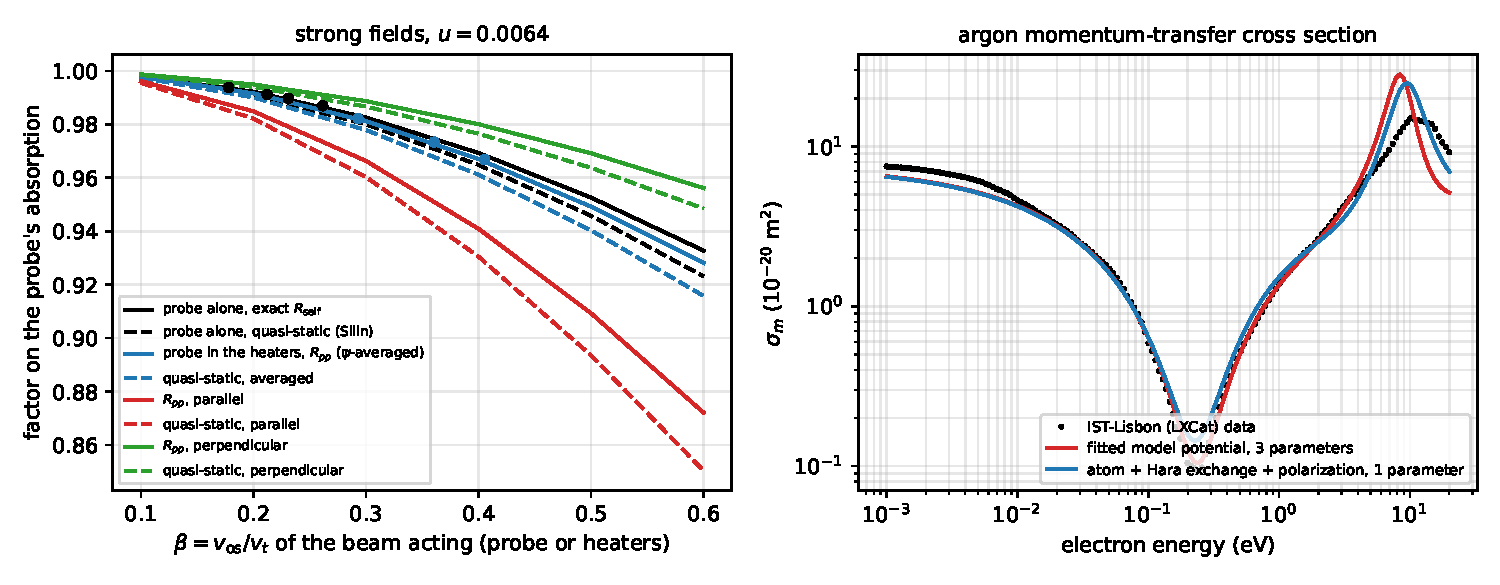
\includegraphics[width=\textwidth]{chapters/lad/v2_fig.pdf}
\caption{Left: the strong-field factors on a probe's absorption at $u=0.0064$ against
$\beta=\vos/v_t$ of the beam that acts. Black: the probe's own field, exact
(Eq.~(\ref*{lad:eq:Rself})) and quasi-static (Silin). Colours: the probe inside the heaters'
quiver, Eq.~(\ref*{lad:eq:Rpp}), averaged over the polarizations (blue), parallel (red) and
perpendicular (green), exact (solid) and in the quasi-static drag picture (dashed). Dots:
the four hydrogen shots. Right: the momentum-transfer cross section of argon from the
IST-Lisbon data, from the three-parameter model potential of Eq.~(\ref*{lad:eq:model}), and from
the Hartree--Fock atom with Hara's exchange and one fitted cutoff.}
\label{lad:fig:v2}
\end{figure}

\subsection{The anisotropy}
\label{lad:sec:aniso}
A linearly polarized field heats along its polarization, and the distribution acquires a
part of degree 2 in the angle, $f=f_0+f_2(v)P_2(\hat{\mathbf v}\cdot\boldsymbol\epsilon)$. Its direct
effect on the absorption of the same beam is
\begin{equation}
\frac{\delta P}{P}=-\frac25\,\frac{\vos^2}{v_t^2}\,Q,\qquad
Q=\int_0^\infty\frac{f_2(v)}{(\vos^2/3v_t^2)\,f_0(0)}\,\frac{\dd v}{v},
\label{lad:eq:aniso}
\end{equation}
with $\vos$ the probe's own quiver velocity. In the Lorentz limit, $Z\gg1$, the field drives $f_2$
through the ion collisions and the same collisions relax it, $f_2=S_2/3\nu_{ei}$, and for the
self-similar heated distribution $Q$ is a number of order one, 1.32, 1.03, 0.93 and 0.87 at the
$\alpha$ of the four shots. Two corrections enter. The drive is inverse bremsstrahlung and carries
the logarithm $\Lambda_1$ with the dynamic cutoff, while the relaxation of the quasi-static $f_2$ is
pitch-angle scattering and carries the transport logarithm $\ln(\lambda_{De}/b_{\min})$ of Sec.~\ref{lad:sec:drude}, 8.10 to
8.36 at the shots: $f_2$ is smaller by $\Lambda_1/\Lambda_{\rm tr}=0.63$ to 0.71. And at $Z=1$ the
electron--electron collisions relax $f_2$ as well. With the test-particle collision operator on a
Maxwellian background \cite{lad:Rosenbluth1957}, in units of $4\pi n_ee^4\Lambda_{\rm tr}/m^2v_t^3$ and with
$w=v/v_t$, $x=w^2/2$ and $\psi(x)={\rm erf}\sqrt x-2(x/\pi)^{1/2}e^{-x}$, $f_2$ solves
\begin{equation}
3\Big(\frac{Z}{w^3}+\nu_D\Big)f_2-\frac{1}{w^2}\frac{\dd}{\dd w}\Big[w^2\frac{\psi}{w^3}\Big(\frac{\dd f_2}{\dd w}+wf_2\Big)\Big]
=\frac{3Z}{w^3}\,\frac{\Lambda_1}{\Lambda_{\rm tr}}\,S_2,\qquad
\nu_D=\frac{(1-1/2x)\psi+\psi'}{w^3},
\label{lad:eq:f2ee}
\end{equation}
with the drive $S_2$ of the Lorentz limit. The operator keeps the Maxwellian, and for fast
electrons at $Z=1$ the deflection by electrons equals that by ions, as it must \cite{lad:Spitzer1953}.
For a Maxwellian drive the electron--electron collisions lower $Q$ by a factor 0.77 to 0.80 at the
hydrogen shots and 0.94 to 0.96 at the mixture shots, where $Z_{\rm eff}\approx5$. Applied to the
self-similar $Q$, the direct effect is 1.30, 0.76, 1.02 and 1.15\,\% at the four hydrogen shots,
against 2.3, 1.3, 2.0 and 2.4\,\% in the Lorentz limit with one logarithm, and 0.32 to 1.07\,\% at the
mixture shots. The feedback of $f_2$ on the isotropic part and the field-particle part of the
electron--electron operator are not computed; the direct part is.

\subsection{The plasma ladder at the hydrogen point}
\label{lad:sec:hpoint}

\begin{table}[ht]
\caption{The electron--ion ladder at the hydrogen point ($n_e/n_c=0.020$, $T_e=0.36$~keV,
$T_i=0.05$~keV, 526.7~nm). The logarithm after each rung and its change against $\Lambda_1$.}
\label{lad:tab:plasma}
\begin{center}
\begin{tabular}{lL{4.6cm}ccc}
\toprule
Sec. & Adds & Parameter & $\Lambda$ & against $\Lambda_1$ (\%)\\
\midrule
\ref*{lad:sec:drude} & Drude--Spitzer, cutoffs by hand & --- & 8.228 & $+40.9$\\
\ref*{lad:sec:quantum} & quantum logarithm, dynamic cutoff & $u$, $\omega/\omega_p$ & 5.839 & 0\\
\ref*{lad:sec:escreen} & screening by the electrons & $\omega_p/\omega$ & 5.832 & $-0.13$\\
\ref*{lad:sec:ions} & correlations of the ions & $a^{1/2}$, $\Gamma_{ii}$ & 5.717 & $-2.08$\\
\ref*{lad:sec:strong} & strong collisions & $\eta_t$ & 5.678 & $-2.77$\\
\ref*{lad:sec:strong} & cross term with the medium & $\eta_t\,b_{\max}/\lambda$ & 5.681 to 5.687 & $-2.71$ to $-2.60$\\
\bottomrule
\end{tabular}
\end{center}
\end{table}

The rungs of Secs.~\ref{lad:sec:langdon} to \ref{lad:sec:aniso} multiply the absorption rather than the logarithm (Sec.~\ref{lad:sec:standard}).

\section{The electron--atom ladder}
\label{lad:sec:gas}

In a weakly ionized gas the electrons absorb mostly while they collide with atoms. For
$\omega$ much larger than the momentum-transfer collision frequency $\nu_m(v)=n_a\sigma_m(v)v$
the Lorentz-gas conductivity gives, for any isotropic $F$ normalized to one,
$\nueff=-(4\pi/3)\int_0^\infty v^3\nu_m(v)\,\partial_vF\,\dd v$.

\subsection{Drude with a mean collision frequency}
\label{lad:sec:meannu}
$\nueff=\langle\nu_m\rangle=n_a\langle\sigma_mv\rangle$ over the Maxwellian. This is the
usual input of a Drude model.

\subsection{The energy-dependent kernel}
\label{lad:sec:kernel}
For a Maxwellian, $\partial_vF=-(v/v_t^2)F$ and
\begin{equation}
\nueff=\frac{\langle\nu_mv^2\rangle}{3v_t^2}=\Big\langle\nu_m\,\frac{2\varepsilon}{3\kB T_e}\Big\rangle,
\label{lad:eq:kernel}
\end{equation}
with $\varepsilon=mv^2/2$, which reduces to $\langle\nu_m\rangle$ of Sec.~\ref{lad:sec:meannu} only for a constant $\nu_m$. The ratio to $\langle\nu_m\rangle$ is
$4/3$ for a constant $\sigma_m$. The IST-Lisbon momentum-transfer cross section of argon
\cite{lad:Alves2014,lad:Yamabe1983,lad:Pitchford2016} has its Ramsauer minimum near 0.25~eV, and with it the
ratio is 0.836 at 300~K and 2.02 at 1.08~eV. A Drude model with a mean collision frequency
is wrong by up to a factor of two here. Parameter: the logarithmic slope of $\sigma_m(\varepsilon)$.
By the low-energy theorem of Low \cite{lad:Low1958} and the formula of Kroll and Watson
\cite{lad:KrollWatson1973}, this kernel is exact for soft photons, $\hbar\omega\ll\varepsilon$, and
the atom enters only through $\sigma_m$.

\subsection{Exact phase shifts}
\label{lad:sec:phases}
When $\hbar\omega$ is comparable with the electron energy the free--free cross section depends
on more than $\sigma_m$. It is computed from the acceleration-form dipole matrix elements
between exact partial waves of a model potential, here
\begin{equation}
V(r)=-\frac{Z}{r}\,\frac{1}{1+H(e^{r/d}-1)}-\frac{\alpha_d}{2(r^2+r_c^2)^2}
\label{lad:eq:model}
\end{equation}
in atomic units, with the screening function of Green, Sellin and Zachor \cite{lad:GSZ1969},
$Z=18$ and the polarizability $\alpha_d=11.083$ \cite{lad:Schwerdtfeger2019}. Its parameters,
$H=4.321$, $d=0.7869$ and $r_c=0.8266$, minimize the rms of $\ln\sigma_m$ against the IST-Lisbon
set over 36 energies from 0.003 to 4~eV (rms 0.081), and it binds the three $s$ and two $p$
orbitals of argon. With $G(\varepsilon)$ the ratio of the exact cross section to its soft-photon
limit, the ratio of the quantum to the classical absorption coefficient is
\begin{equation}
R=\frac{1-e^{-u}}{u}\,\frac{\langle\sigma_mG\rangle_w}{\langle\sigma_m\rangle_w},
\label{lad:eq:R}
\end{equation}
with the weight $\varepsilon^2e^{-\varepsilon/\kB T_e}$ of Eq.~\eqref{lad:eq:kernel}. Parameter: $u$. For
argon $R=0.9984$ at 1~THz and 0.9749 at 4~THz for 300~K electrons, and 0.591 at 28.3~THz, the
CO$_2$ laser; at 1.08~eV it stays within $10^{-3}$ of one at all three frequencies.

{\noindent}\emph{From the atom.} Equation~\eqref{lad:eq:model} is fitted to $\sigma_m$ with three
parameters, so the mid-infrared value rests on the fit. A potential built from the atom
replaces it: the static field of the closed-shell Hartree--Fock atom, $V_{st}=-Z/r+V_H$, whose
total energy is $-526.831$ against the Hartree--Fock limit $-526.818$~hartree, plus a local
exchange, plus the same polarization tail with the single parameter $r_c$. The semiclassical
exchange of Furness and McCarthy, $V_{ex}=\tfrac12(E-V_{st})-\tfrac12[(E-V_{st})^2+4\pi\rho]^{1/2}$
with $\rho$ the electron density \cite{lad:FurnessMcCarthy1973}, is far too attractive at these
energies: no $r_c$ brings its $\sigma_m$ within a factor of 4.5 of the data. The free-electron-gas
exchange of Hara \cite{lad:Hara1967},
\begin{equation}
V_{ex}=-\frac{k_F}{\pi}\Big[1+\frac{1-\eta^2}{2\eta}\ln\Big|\frac{1+\eta}{1-\eta}\Big|\Big],\qquad
k_F=(3\pi^2\rho)^{1/3},\quad\eta=\frac{(k^2+2I+k_F^2)^{1/2}}{k_F},
\label{lad:eq:hara}
\end{equation}
with $I$ the ionization energy, does reproduce the Ramsauer region: with $r_c=$1.548 the rms of
$\ln\sigma_m$ over the same 36 energies is 0.172, against 0.081 for the three-parameter fit,
and the minimum lies at 0.226~eV against about 0.25~eV in the data; over 0.003 to 20~eV the rms
is 0.215. With this potential $R$ at 300~K is 0.9986 at 1~THz, 0.9744 at 4~THz and 0.566 at
28.3~THz, against 0.9984, 0.9749 and 0.591 for Eq.~\eqref{lad:eq:model}; at 1.08~eV it is 1.0009
at 28.3~THz. The exchange depends on the energy, and the matrix elements between $k$ and $k'$
use the potential at the mean energy. The mid-infrared reduction is therefore a property of
the phase shifts that any potential reproducing $\sigma_m$ shares, not of the fit.

\subsection{Polarization bremsstrahlung}
\label{lad:sec:polbrems}
The field of the electron induces a dipole $\alpha_d\hat{\mathbf r}/r^2$ (atomic units) in the atom,
which radiates together with the electron. In the acceleration form, where the electron's dipole
matrix element is that of $V'(r)/\omega^2$, the radial force $V'(r)$ becomes
$V'(r)-\omega^2\alpha_d/(r^2+r_c^2)$, with the cutoff $r_c$ of the polarization tail.
Parameter: $\alpha_d\omega^2$ against the atomic force. For argon with Eq.~\eqref{lad:eq:model} it
changes $R$ by $-0.03$\,\% at 1~THz and $-0.43$\,\% at 4~THz for 300~K electrons, and by
$-13.0$\,\% at 28.3~THz, where $R$ becomes 0.514; at 1.08~eV the change is below 0.1\,\%. With
the potential from the atom, $R$ at 28.3~THz and 300~K becomes 0.491.

\subsection{Multiple collisions}
\label{lad:sec:multiple}
An electron can scatter on two atoms in a row. The kinetic equation counts every collision with
its own photon-exchange cross section whatever collision follows, so sequences of collisions add
nothing to the absorption of a gas. They do add a signal proportional to the square of the
density in laser-assisted scattering experiments, which may explain why photon exchange in argon
in CO$_2$-laser fields was measured far above the Kroll--Watson prediction
\cite{lad:WallbankHolmes1994,lad:Rabadan1996}. That anomaly is a question about single-collision cross
sections, and measurements at several target densities would settle it.

\begin{table}[ht]
\caption{The electron--atom ladder for argon. $\nueff/\langle\nu_m\rangle$ is the ratio of the collision frequency
of Eq.~(\ref*{lad:eq:kernel}) to that of Sec.~\ref*{lad:sec:meannu}; $R$ is Eq.~(\ref*{lad:eq:R}) without and with polarization
bremsstrahlung (Secs.~\ref*{lad:sec:phases} and \ref*{lad:sec:polbrems}), for the fitted potential of Eq.~(\ref*{lad:eq:model}) and for the potential from the
atom with Hara's exchange.}
\label{lad:tab:gas}
\begin{center}
\begin{tabular}{ccccccc}
\toprule
& & & \multicolumn{2}{c}{fitted potential} & \multicolumn{2}{c}{atom + Hara exchange}\\
\cmidrule(lr){4-5}\cmidrule(lr){6-7}
$T_e$ & $\nueff/\langle\nu_m\rangle$ & $f$ (THz) & $R$ (Sec.~\ref*{lad:sec:phases}) & $R$ (Sec.~\ref*{lad:sec:polbrems}) & $R$ (Sec.~\ref*{lad:sec:phases}) & $R$ (Sec.~\ref*{lad:sec:polbrems})\\
\midrule
300~K & 0.836 & 1 & 0.9984 & 0.9981 & 0.9986 & 0.9983\\
 & & 4 & 0.9749 & 0.9707 & 0.9744 & 0.9702\\
 & & 28.3 & 0.591 & 0.514 & 0.566 & 0.491\\
1.08~eV & 2.02 & 1 & 1.0000 & 1.0000 & 1.0000 & 1.0000\\
 & & 4 & 1.0000 & 1.0000 & 1.0000 & 1.0001\\
 & & 28.3 & 1.0008 & 1.0018 & 1.0009 & 1.0019\\
\bottomrule
\end{tabular}
\end{center}
\end{table}

\subsection{One collision against two}
\label{lad:sec:onetwo}
The anomaly of Sec.~\ref{lad:sec:multiple} needs the size of the single-collision photon exchange where Kroll and Watson
give zero, $\boldsymbol\epsilon\cdot\mathbf Q=0$. To first order in the field and exactly in the
atomic potential, the one-photon amplitude between the scattering states of momenta $\mathbf k_i$
and $\mathbf k_f$ is, in the acceleration form and atomic units,
\begin{equation}
M=\sum_{l,\,l'=l\pm1}i^{\,l-l'}e^{i(\delta^f_{l'}+\delta^i_l)}R_{l'l}
\sum_{mm'}Y_{l'm'}(\hat{\mathbf k}_f)\,\langle l'm'|\boldsymbol\epsilon\cdot\hat{\mathbf r}|lm\rangle\,Y^*_{lm}(\hat{\mathbf k}_i),\qquad
R_{l'l}=\frac{1}{\omega^2}\int_0^\infty u_{k_fl'}V'u_{k_il}\,\dd r,
\label{lad:eq:Mamp}
\end{equation}
with radial waves of unit amplitude, and the ratio of the one-photon signal to the elastic one in
a field of amplitude $E_0$ is
\begin{equation}
\frac{\dd\sigma_{+1}}{\dd\sigma_{\rm el}}=\frac{16\pi^2E_0^2|M|^2}{k_i^3k_f\,|f_{\rm el}|^2},
\label{lad:eq:ratio}
\end{equation}
with $f_{\rm el}$ the elastic amplitude. Three properties check it. Averaged over the polarization
and integrated over $\hat{\mathbf k}_f$, $|M|^2$ gives back the integrated free--free cross section
of Sec.~\ref{lad:sec:phases}, to $5\times10^{-14}$. At 0.3~THz, where the photon is soft, Eq.~\eqref{lad:eq:ratio} with
$\boldsymbol\epsilon\parallel\mathbf Q$ equals the Kroll--Watson value $(k_f/k_i)(\boldsymbol\epsilon\cdot\mathbf Q)^2a_0^2/4$
to $6.4\times10^{-4}$. In the geometry with $\boldsymbol\epsilon$ normal to the scattering plane it
vanishes to $10^{-31}$, as the reflection symmetry of Sec.~\ref{lad:sec:multiple} requires. The partial waves are taken to
$l=22$, with the polarization tail of the elastic amplitude summed in the Born approximation,
$\delta_l=\pi\alpha_dk^2/[(2l-1)(2l+1)(2l+3)]$, beyond \cite{lad:OMalley1961}; going to $l=26$ changes the
signal by $4.8\times10^{-3}$ and halving the radial step by $3.5\times10^{-5}$. In the expansion in the
field the next term carries $a_0k\,\hbar\omega/E\approx0.03$ at 10~eV.

In the in-plane geometry, $\boldsymbol\epsilon$ in the scattering plane and perpendicular to
$\mathbf Q$, argon at 10~eV in a CO$_2$ laser at $10^8$~W\,cm$^{-2}$ gives a one-photon signal of
$2.25\times10^{-3}$ of the elastic one at $90^\circ$ with the fitted potential of Eq.~\eqref{lad:eq:model} and
$1.23\times10^{-3}$ with the potential from the atom; $1.72\times10^{-3}$ and $1.00\times10^{-3}$ at 8~eV,
$3.80\times10^{-4}$ and $3.37\times10^{-4}$ at 20~eV. This is the dipole amplitude $f_D$ of the in-plane
geometry, 37 and 20 times the nondipole term, which with the laser beam along $\mathbf Q$ gives
$(k_f/k_i)J_1^2(x_1)=6.09\times10^{-5}$ with $x_1=a_0(\hat{\mathbf k}\cdot\mathbf Q)(\boldsymbol\epsilon\cdot\bar{\mathbf v})/c=0.0156$,
$\bar{\mathbf v}$ the mean of the two velocities. To first order in $v/c$ the in-plane amplitude is
$f_D+f_N\cos\varphi$, with $\varphi$ the angle between the laser direction $\hat{\mathbf k}$ and $\mathbf Q$ (the
reflection through the scattering plane removes a term in $\sin\varphi$), so the interference
$2{\rm Re}(f_D^*f_N)\cos\varphi$ can move the in-plane signal by up to $2|f_N/f_D|$, 33 and 44\,\% of
$|f_D|^2$, as the laser direction turns. The polarization bremsstrahlung of
Sec.~\ref{lad:sec:polbrems} changes the in-plane signal by at most 0.6\,\%, since its first order vanishes with
$\boldsymbol\epsilon\cdot\mathbf Q$. In absolute terms the single-collision cross section at 10~eV stays
below 1.3\,\% of the elastic one at $90^\circ$ at every angle; its ratio to the elastic signal rises only
where the elastic cross section has a minimum, to $1.19\times10^{-2}$ and 0.18 at $120^\circ$, and
there the two potentials disagree.

Double scattering in the target is computed with the same potentials, for the gas cylinder of
radius 1~mm and length 2~mm about the beam: each collision follows Kroll and Watson, the second
collision returns the photon count to one, and the signal per incident electron is $n^2D_1$ with
\begin{equation}
D_1=\int\dd\Omega_1\,G(\hat{\mathbf u}_1)\,\frac{\dd\sigma_{\rm el}}{\dd\Omega}(\hat{\mathbf z}\cdot\hat{\mathbf u}_1)\,
\frac{\dd\sigma_{\rm el}}{\dd\Omega}(\hat{\mathbf u}_1\cdot\hat{\mathbf u}_d)\sum_\ell J_\ell^2(\xi)J_{1-\ell}^2(\xi),\qquad
\xi=ka_0\,\boldsymbol\epsilon\cdot(\hat{\mathbf u}_1-\hat{\mathbf z}),
\label{lad:eq:D1}
\end{equation}
where $G$ is the path length in the gas integrated along the beam. Relative to the single-collision
elastic signal it is $nd_1$, with $d_1=D_1/(L\,\dd\sigma_{\rm el}/\dd\Omega)$. At $90^\circ$,
$d_1=3.27\times10^{-17}$ and $2.77\times10^{-17}$~cm$^3$ in the in-plane geometry and $4.50\times10^{-17}$
and $4.26\times10^{-17}$~cm$^3$ in the normal geometry. The single collision and the double scattering
are therefore equal at $n^*=6.9\times10^{13}$ and $4.5\times10^{13}$~cm$^{-3}$ at $90^\circ$, at $5.3$ and
$2.8\times10^{13}$~cm$^{-3}$ at $60^\circ$ and at $2.4$ and $2.9\times10^{13}$~cm$^{-3}$ at $120^\circ$: at the
densities of the targets used, the two mechanisms are of the same size in the in-plane geometry.
In the normal geometry the single collision is absent. Both rise toward the minima of the elastic
cross section, both stay one to two orders of magnitude below the measured 12\,\% away from them,
and a density scan in the two geometries separates them: an intercept in the in-plane geometry
only, a slope in both. The two potentials give $\sigma_m(10~{\rm eV})$ 33 and 63\,\% above the data,
so the numbers at 10~eV carry that uncertainty; their crossover densities $n^*$ agree within a
factor 2.

\begin{table}[ht]
\caption{Argon at 28.3~THz and $10^8$~W\,cm$^{-2}$: the exact single-collision one-photon signal
relative to the elastic one in the in-plane geometry with $\boldsymbol\epsilon\perp\mathbf Q$, double
scattering $d_1$ in the same geometry, and the density $n^*$ at which the two are equal, for the
fitted potential and the potential from the atom, at 10~eV.}
\label{lad:tab:onetwo}
\begin{center}
\begin{tabular}{ccccccc}
\toprule
& \multicolumn{3}{c}{fitted potential} & \multicolumn{3}{c}{atom + Hara exchange}\\
\cmidrule(lr){2-4}\cmidrule(lr){5-7}
angle & single & $d_1$ (cm$^3$) & $n^*$ (cm$^{-3}$) & single & $d_1$ (cm$^3$) & $n^*$ (cm$^{-3}$)\\
\midrule
$60^\circ$ & $2.93\times10^{-3}$ & $5.51\times10^{-17}$ & $5.32\times10^{13}$ & $1.61\times10^{-3}$ & $5.79\times10^{-17}$ & $2.79\times10^{13}$\\
$90^\circ$ & $2.25\times10^{-3}$ & $3.27\times10^{-17}$ & $6.89\times10^{13}$ & $1.23\times10^{-3}$ & $2.77\times10^{-17}$ & $4.45\times10^{13}$\\
$120^\circ$ & $1.19\times10^{-2}$ & $5.05\times10^{-16}$ & $2.36\times10^{13}$ & $1.81\times10^{-1}$ & $6.36\times10^{-15}$ & $2.85\times10^{13}$\\
\bottomrule
\end{tabular}
\end{center}
\end{table}

\section{Putting the rungs together}
\label{lad:sec:standard}

\subsection{The two kinds of scatterer add}
\label{lad:sec:add}
Electron--ion and electron--atom collisions are separate binary events, and
electron--electron collisions radiate no dipole radiation, since two electrons have the same
charge-to-mass ratio. So $\nueff=\nu_T\Lambda+\nu_{ea}$. In argon at 1~atm and 300~K, at 1~THz,
the two are equal at $n_e=1.0\times10^{13}$~cm$^{-3}$ for 300~K electrons, the Ramsauer minimum
making the atoms weak scatterers, and at $1.0\times10^{16}$~cm$^{-3}$ for 1.08~eV electrons, close
to the critical density $1.24\times10^{16}$~cm$^{-3}$ at that frequency.

\subsection{The standard model}
\label{lad:sec:stdmodel}
Collecting the rungs, the absorption coefficient of a probe is Eq.~\eqref{lad:eq:K} with
\begin{equation}
\boxed{\;\begin{aligned}
\nueff={}&\nu_T\Big[\Lambda_{2,3}(r,u,\{Z_i\})+\Delta\Lambda_4(\eta_t,u)+C\Big]\,
f_L(\alpha)\,C_L\big(m(\alpha),u\big)\\
&\times\frac{f_{sp}}{f_L}\,R_{\rm self}(\beta_p,u)\,R_{pp}(\beta_h,u)\,\Big(1+\frac{\delta P}{P}\Big)\\
&+\;n_a\Big\langle\sigma_mv\,\frac{2\varepsilon}{3\kB T_e}\Big\rangle R(u),
\end{aligned}\;}
\label{lad:eq:standard}
\end{equation}
where $\Lambda_{2,3}$ is Eq.~\eqref{lad:eq:DO} in the form of Eq.~\eqref{lad:eq:Lam2} with the charge structure
factor of the ion mixture from Eq.~\eqref{lad:eq:hnc}, $\Delta\Lambda_4=\Lambda_4-\Lambda_1$, $C$ is the cross
term of Eq.~\eqref{lad:eq:cross}, $C_L$ is the second factor of Eq.~\eqref{lad:eq:langdon}, $f_{sp}$ is
Eq.~\eqref{lad:eq:fsp}, $R_{\rm self}$ and $R_{pp}$ are Eqs.~\eqref{lad:eq:Rself} and \eqref{lad:eq:Rpp}, $\delta P/P$ is
Eq.~\eqref{lad:eq:aniso} with $f_2$ from Eq.~\eqref{lad:eq:f2ee}, and the last term is Eq.~\eqref{lad:eq:kernel} times $R$ of Secs.~\ref{lad:sec:phases} and \ref{lad:sec:polbrems}.
Products of factors are a first-order approximation in each correction.

\subsection{The budgets of the fourteen shots}
\label{lad:sec:budgets}
The ladder shares the rungs of Secs.~\ref{lad:sec:quantum}, \ref{lad:sec:strong} and \ref{lad:sec:langdon} with the composite of Turnbull et al. What it adds is the product
\begin{equation}
X=\frac{\Lambda_{2,3}+\Delta\Lambda_4+C}{\Lambda_1+\Delta\Lambda_4}\;\frac{f_{sp}}{f_L}\;R_{\rm self}\;R_{pp}\;
\Big(1+\frac{\delta P}{P}\Big),
\label{lad:eq:X}
\end{equation}
listed shot by shot in Tables~\ref{lad:tab:budget} and \ref{lad:tab:mixbudget}. The exact-Gaunt correction
$\Delta\Lambda_4$ and the cross term $C$ are weighted by $n_iZ_i^2$ over the ion species: $\Delta\Lambda_4$ is
$-0.67$ to $-0.88$\,\% of $\Lambda_1$ for hydrogen and $-8.3$ to $-12.1$\,\% for the mixtures, where the
nitrogen ions carry it, and $C=+0.0098$ for the protons and $+0.0383$ for the nitrogen ions. For
hydrogen $X$ is 0.916 to 0.926, with a mean of 0.921; for the mixtures it is 0.871 to 0.911, with a mean of 0.895.

\begin{table}[ht]
\caption{The budget of the four hydrogen shots: the logarithm factor of Eq.~(\ref*{lad:eq:X}), the speckle
factor, the strong-field factors, the anisotropy, their product $X$ of Eq.~(\ref*{lad:eq:X}) and the ladder against
the measurements, $1.29X$. The fitted factor $f_{sc}$ of Turnbull et al.\ is listed for comparison.}
\label{lad:tab:budget}
\begin{center}
\begin{tabular}{ccccccccc}
\toprule
shot & logarithm & $f_{sp}/f_L$ & $R_{\rm self}$ & $R_{pp}$ & $-\delta P/P$ & $X$ & ladder/data & $f_{sc}$\\
\midrule
102727 & 0.983 & 0.955 & 0.991 & 1 & 0.0130 & 0.918 & 1.185 & 0.837\\
104031 & 0.979 & 0.977 & 0.994 & 0.982 & 0.0076 & 0.926 & 1.195 & 0.827\\
106310 & 0.993 & 0.973 & 0.990 & 0.974 & 0.0102 & 0.922 & 1.189 & 0.884\\
106311 & 0.998 & 0.972 & 0.987 & 0.967 & 0.0115 & 0.916 & 1.181 & 0.927\\
\bottomrule
\end{tabular}
\end{center}
\end{table}

\begin{table}[ht]
\caption{The budget of the ten nitrogen--hydrogen shots, as Table~\ref*{lad:tab:budget}; the ladder
against the measurements is $1.07X$.}
\label{lad:tab:mixbudget}
\begin{center}
\begin{tabular}{ccccccccc}
\toprule
shot & logarithm & $f_{sp}/f_L$ & $R_{\rm self}$ & $R_{pp}$ & $-\delta P/P$ & $X$ & ladder/data & $f_{sc}$\\
\midrule
102729 & 0.944 & 0.946 & 0.997 & 1 & 0.0049 & 0.886 & 0.948 & 0.911\\
102737 & 0.949 & 0.965 & 0.996 & 0.994 & 0.0047 & 0.903 & 0.966 & 0.915\\
102738 & 0.936 & 0.986 & 0.997 & 0.981 & 0.0032 & 0.899 & 0.962 & 0.896\\
104035 & 0.949 & 0.977 & 0.997 & 0.988 & 0.0037 & 0.910 & 0.973 & 0.898\\
104037 & 0.953 & 0.949 & 0.997 & 1 & 0.0045 & 0.898 & 0.961 & 0.904\\
104041 & 0.957 & 0.944 & 0.996 & 1 & 0.0064 & 0.894 & 0.956 & 0.917\\
106315 & 0.949 & 0.942 & 0.994 & 1 & 0.0080 & 0.881 & 0.943 & 0.902\\
106316 & 0.968 & 0.942 & 0.994 & 1 & 0.0084 & 0.898 & 0.961 & 0.943\\
106317 & 0.987 & 0.942 & 0.991 & 1 & 0.0107 & 0.911 & 0.975 & 0.969\\
106319 & 0.928 & 0.946 & 0.997 & 1 & 0.0047 & 0.871 & 0.932 & 0.879\\
\bottomrule
\end{tabular}
\end{center}
\end{table}

\begin{figure}[ht]
\centering
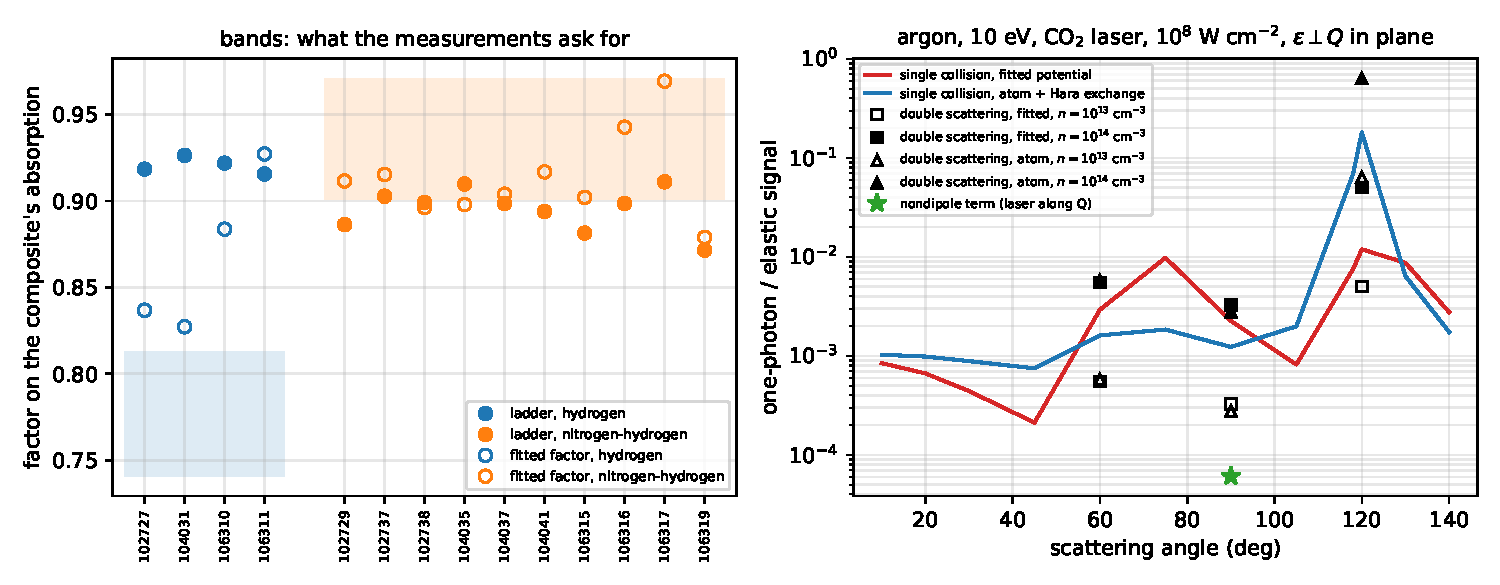
\includegraphics[width=\textwidth]{chapters/lad/v3_fig.pdf}
\caption{Left: per shot, the factor $X$ of Eq.~(\ref*{lad:eq:X}) that the ladder applies beyond the composite
of Turnbull et al.\ (filled) and their fitted screening factor $f_{sc}$ (open), against the factor the
measurements ask for, $1/(1.29\pm0.06)$ for hydrogen and $1/(1.07\pm0.04)$ for the mixtures (bands).
Right: argon at 10~eV in a CO$_2$ laser at $10^8$~W\,cm$^{-2}$, in the in-plane geometry with
$\boldsymbol\epsilon\perp\mathbf Q$: the exact single-collision one-photon signal relative to the elastic
one for the two potentials (lines), double scattering in the target at $10^{13}$ and $10^{14}$~cm$^{-3}$
(markers), and the nondipole term (star).}
\label{lad:fig:v3}
\end{figure}

\subsection{Rules against counting an effect twice}
\label{lad:sec:rules}
\begin{enumerate}
\item \emph{One upper cutoff.} The dynamic cutoff $v_t/\omega$ of Sec.~\ref{lad:sec:quantum} and the Debye length of Sec.~\ref{lad:sec:drude} are
two models of the same long-range cut. Electron screening enters through $\varepsilon$ in Sec.~\ref{lad:sec:escreen}, never
as a second cutoff.
\item \emph{One account of the ions.} The rung of Sec.~\ref{lad:sec:ions} and a fitted screening factor both describe how the ions
modify the long-range part of the logarithm. Applying $f_{sc}$ on top of that rung counts the ion
correlations twice.
\item \emph{Strong collisions once.} The exact Gaunt factor of Sec.~\ref{lad:sec:strong} already contains the Born term;
it is added as $\Lambda_4-\Lambda_1$ to the medium logarithm, not multiplied by it, and the
cross term of Eq.~\eqref{lad:eq:cross} is the only further piece.
\item \emph{One logarithm throughout.} The Langdon factor of Sec.~\ref{lad:sec:langdon} must use the same velocity-dependent
logarithm as Sec.~\ref{lad:sec:quantum} or \ref{lad:sec:strong}; Langdon's fit alone assumes a fixed one.
\item \emph{The field once per beam.} $R_{\rm self}$ holds the probe's own quiver, $R_{pp}$ the
heaters'; the Langdon parameter $\alpha$ of Sec.~\ref{lad:sec:langdon} takes the overlapped intensity because it describes
the time-averaged distribution, which every beam shapes. Neither replaces the other.
\item \emph{No separate term for collision sequences.} Double scattering is already in the
kinetic equation (Sec.~\ref{lad:sec:multiple}).
\item \emph{Electron--electron collisions shape, they do not absorb.} They enter through $\alpha$ in
Sec.~\ref{lad:sec:langdon} and through the relaxation of $f_2$ in Sec.~\ref{lad:sec:aniso}, not as a third scatterer.
\item \emph{Two logarithms in the anisotropy.} The field drives $f_2$ with the inverse-bremsstrahlung
logarithm, and collisions relax it with the transport logarithm; using one for both overstates the
anisotropy by $\Lambda_{\rm tr}/\Lambda_1\approx1.5$.
\end{enumerate}

\section{Have the models improved?}
\label{lad:sec:verdict}

{\noindent}\emph{Plasma.} Against the composite of Turnbull et al.\ without their screening factor,
which is $1.29\pm0.06$ times the measured absorption of the hydrogen shots and $1.07\pm0.04$ times
that of the mixture shots, the ladder is
\begin{equation}
\boxed{\;\frac{K_{\rm ladder}}{K_{\rm measured}}=
\begin{cases}
1.07\,\bar X_{\rm N_2/H_2}=1.07\times0.895=0.96\pm0.04 & \text{(ten nitrogen--hydrogen shots)},\\[2pt]
1.29\,\bar X_{\rm H_2}=1.29\times0.921=1.19\pm0.06 & \text{(four hydrogen shots)}.
\end{cases}\;}
\label{lad:eq:verdict}
\end{equation}
For the mixtures the ladder, with no fitted parameter, agrees with the measurements as well as the
fitted composite of Turnbull et al., $1.00\pm0.04$ \cite{lad:Turnbull2024}. In these plasmas the fitted
factor and the computed correlations of the ions do the same thing, 0.879 to 0.969 against a medium
factor of 0.930 to 0.982, because the heavy ions make the correlations strong. For hydrogen they part:
the fitted factor lowers the absorption by 7 to 17\,\%, the medium by 0.4 to 2.2\,\%, and the
hypernetted chain confirms Debye--H\"uckel to $2\times10^{-4}$ at $\Gamma_{ii}=0.02$. \emph{The ladder
explains the mixture shots and leaves the hydrogen shots 19\,\% too absorbing.} Every rung that
could act on hydrogen alone is now computed and small: the anisotropy, which scales as $1/Z$, 0.8 to
1.3\,\%; the strong fields 1 to 5\,\%; the speckles 2.3 to 4.5\,\%. The residual is the size of a 12\,\% error
in $T_e$ or a 9\,\% error in $n_e$ of the hydrogen shots, whose measured absorption, 0.15 to 1.48\,\%, is
the smallest of the data set (0.47 to 5.05\,\% for the mixtures).

{\noindent}\emph{The discriminating measurement.} Helium against hydrogen at the conditions of the
four hydrogen shots, each normalized by the unscreened model of its own charge: the ladder predicts
0.987, 0.985, 0.993 and 0.997, the fitted factor 1.042, 1.044, 1.034 and 1.024. The two differ by 2.7
to 5.8\,\% and move in opposite directions.

{\noindent}\emph{Gas.} Against a Drude model with a mean collision frequency,
\begin{equation}
\boxed{\;\frac{K_{\rm ladder}}{K_{\rm Drude}}=\frac{\langle\nu_m\,2\varepsilon/3\kB T_e\rangle}{\langle\nu_m\rangle}\,R
=0.836\ \text{(300 K)}\ \text{to}\ 2.02\ \text{(1.08 eV)}\ \text{at 1 to 4 THz},\;}
\label{lad:eq:verdictgas}
\end{equation}
where $R$ of Secs.~\ref{lad:sec:phases} and \ref{lad:sec:polbrems} is 0.97 to 1.00 at 1 to 4~THz, and at 28.3~THz $R$ lowers it further, to 0.514
of the classical kernel for 300~K electrons with the fitted potential and 0.491 with the potential
from the atom (Table~\ref{lad:tab:gas}). The single collisions beyond Kroll and Watson are computed
(Table~\ref{lad:tab:onetwo}); they equal double scattering at the densities of the targets used.

\section{What remains open}
\label{lad:sec:open}

\begin{enumerate}
\item \emph{The hydrogen residual.} The ladder accounts for the mixture shots and leaves 19\,\% for
hydrogen, with every hydrogen-specific rung computed. The theory therefore places the residual in
the hydrogen measurements or their plasma conditions, not in the absorption physics; the helium
measurement of Sec.~\ref{lad:sec:verdict} decides between this and a fitted screening length.
\item \emph{The anisotropy beyond its direct part.} The feedback of $f_2$ on the isotropic
distribution and the field-particle part of the electron--electron operator are not computed. They
change the 0.8 to 1.3\,\% of Sec.~\ref{lad:sec:aniso} by a factor of order one, not the residual.
\item \emph{Argon at the elastic minima.} The single-collision and double-scattering signals are
computed; near the minima of the elastic cross section, where the measured photon exchange is
largest, both depend on the depth and the position of the minimum, which the two potentials do not
agree on. A density scan in the in-plane and normal geometries measures both.
\end{enumerate}
Closed here: the ion correlations beyond Debye--H\"uckel (Sec.~\ref{lad:sec:ions}), the strong-collision cross
term at the mixtures' conditions (Sec.~\ref{lad:sec:strong}), the heaters' own strong-field factor and the exact factor at
$\beta\ge1$ (Sec.~\ref{lad:sec:fields}), the anisotropy with two logarithms and electron--electron collisions (Sec.~\ref{lad:sec:aniso}), and the
single-collision photon exchange beyond Kroll and Watson in argon (Sec.~\ref{lad:sec:onetwo}).

\begin{thebibliography}{99}
\raggedright
\bibitem{lad:Atzeni2004} S.~Atzeni and J.~Meyer-ter-Vehn, \emph{The Physics of Inertial Fusion}
(Oxford University Press, Oxford, 2004), doi:\href{https://doi.org/10.1093/acprof:oso/9780198562641.001.0001}{10.1093/acprof:oso/9780198562641.001.0001}.
\bibitem{lad:Turnbull2023} D.~Turnbull \emph{et al.}, Phys. Rev. Lett. \textbf{130}, 145103 (2023),
doi:\href{https://doi.org/10.1103/PhysRevLett.130.145103}{10.1103/PhysRevLett.130.145103}.
\bibitem{lad:Turnbull2024} D.~Turnbull \emph{et al.}, Phys. Plasmas \textbf{31}, 063304 (2024),
doi:\href{https://doi.org/10.1063/5.0203446}{10.1063/5.0203446}.
\bibitem{lad:Kramers1923} H.~A.~Kramers, Phil. Mag. \textbf{46}, 836 (1923),
doi:\href{https://doi.org/10.1080/14786442308565244}{10.1080/14786442308565244}.
\bibitem{lad:KarzasLatter1961} W.~J.~Karzas and R.~Latter, Astrophys. J. Suppl. \textbf{6}, 167 (1961),
doi:\href{https://doi.org/10.1086/190063}{10.1086/190063}.
\bibitem{lad:DawsonOberman1962} J.~Dawson and C.~Oberman, Phys. Fluids \textbf{5}, 517 (1962),
doi:\href{https://doi.org/10.1063/1.1706652}{10.1063/1.1706652}.
\bibitem{lad:Sommerfeld1931} A.~Sommerfeld, Ann. Phys. \textbf{403}, 257 (1931),
doi:\href{https://doi.org/10.1002/andp.19314030302}{10.1002/andp.19314030302}.
\bibitem{lad:vanHoof2014} P.~A.~M.~van~Hoof, R.~J.~R.~Williams, K.~Volk, M.~Chatzikos, G.~J.~Ferland,
M.~Lykins, R.~L.~Porter and Y.~Wang, Mon. Not. R. Astron. Soc. \textbf{444}, 420 (2014),
doi:\href{https://doi.org/10.1093/mnras/stu1438}{10.1093/mnras/stu1438}.
\bibitem{lad:Bloch1933} F.~Bloch, Ann. Phys. (Leipzig) \textbf{408}, 285 (1933),
doi:\href{https://doi.org/10.1002/andp.19334080303}{10.1002/andp.19334080303}.
\bibitem{lad:Langdon1980} A.~B.~Langdon, Phys. Rev. Lett. \textbf{44}, 575 (1980),
doi:\href{https://doi.org/10.1103/PhysRevLett.44.575}{10.1103/PhysRevLett.44.575}.
\bibitem{lad:Matte1988} J.~P.~Matte, M.~Lamoureux, C.~M\"oller, R.~Y.~Yin, J.~Delettrez, J.~Virmont
and T.~W.~Johnston, Plasma Phys. Control. Fusion \textbf{30}, 1665 (1988),
doi:\href{https://doi.org/10.1088/0741-3335/30/12/004}{10.1088/0741-3335/30/12/004}.
\bibitem{lad:KullPlagne2001} H.-J.~Kull and L.~Plagne, Phys. Plasmas \textbf{8}, 5244 (2001),
doi:\href{https://doi.org/10.1063/1.1416182}{10.1063/1.1416182}.
\bibitem{lad:Bornath2001} Th.~Bornath, M.~Schlanges, P.~Hilse and D.~Kremp, Phys. Rev. E \textbf{64},
026414 (2001), doi:\href{https://doi.org/10.1103/PhysRevE.64.026414}{10.1103/PhysRevE.64.026414}.
\bibitem{lad:Decker1994} C.~D.~Decker, W.~B.~Mori, J.~M.~Dawson and T.~Katsouleas, Phys. Plasmas
\textbf{1}, 4043 (1994), doi:\href{https://doi.org/10.1063/1.870874}{10.1063/1.870874}.
\bibitem{lad:Alves2014} L.~L.~Alves, J. Phys.: Conf. Ser. \textbf{565}, 012007 (2014),
doi:\href{https://doi.org/10.1088/1742-6596/565/1/012007}{10.1088/1742-6596/565/1/012007};
IST-Lisbon database, \url{https://www.lxcat.net}.
\bibitem{lad:Yamabe1983} C.~Yamabe, S.~J.~Buckman and A.~V.~Phelps, Phys. Rev. A \textbf{27}, 1345 (1983),
doi:\href{https://doi.org/10.1103/PhysRevA.27.1345}{10.1103/PhysRevA.27.1345}.
\bibitem{lad:Pitchford2016} L.~C.~Pitchford \emph{et al.}, Plasma Process. Polym. \textbf{14}, 1600098
(2016), doi:\href{https://doi.org/10.1002/ppap.201600098}{10.1002/ppap.201600098}.
\bibitem{lad:Low1958} F.~E.~Low, Phys. Rev. \textbf{110}, 974 (1958),
doi:\href{https://doi.org/10.1103/PhysRev.110.974}{10.1103/PhysRev.110.974}.
\bibitem{lad:KrollWatson1973} N.~M.~Kroll and K.~M.~Watson, Phys. Rev. A \textbf{8}, 804 (1973),
doi:\href{https://doi.org/10.1103/PhysRevA.8.804}{10.1103/PhysRevA.8.804}.
\bibitem{lad:GSZ1969} A.~E.~S.~Green, D.~L.~Sellin and A.~S.~Zachor, Phys. Rev. \textbf{184}, 1 (1969),
doi:\href{https://doi.org/10.1103/PhysRev.184.1}{10.1103/PhysRev.184.1}.
\bibitem{lad:Schwerdtfeger2019} P.~Schwerdtfeger and J.~K.~Nagle, Mol. Phys. \textbf{117}, 1200 (2019),
doi:\href{https://doi.org/10.1080/00268976.2018.1535143}{10.1080/00268976.2018.1535143}.
\bibitem{lad:FurnessMcCarthy1973} J.~B.~Furness and I.~E.~McCarthy, J. Phys. B: At. Mol. Phys. \textbf{6},
2280 (1973), doi:\href{https://doi.org/10.1088/0022-3700/6/11/021}{10.1088/0022-3700/6/11/021}.
\bibitem{lad:Hara1967} S.~Hara, J. Phys. Soc. Jpn. \textbf{22}, 710 (1967),
doi:\href{https://doi.org/10.1143/JPSJ.22.710}{10.1143/JPSJ.22.710}.
\bibitem{lad:WallbankHolmes1994} B.~Wallbank and J.~K.~Holmes, J. Phys. B: At. Mol. Opt. Phys.
\textbf{27}, 5405 (1994),
doi:\href{https://doi.org/10.1088/0953-4075/27/21/027}{10.1088/0953-4075/27/21/027}.
\bibitem{lad:Rabadan1996} I.~Rabad\'an, L.~M\'endez and A.~S.~Dickinson, J. Phys. B: At. Mol. Opt. Phys.
\textbf{29}, L801 (1996),
doi:\href{https://doi.org/10.1088/0953-4075/29/22/004}{10.1088/0953-4075/29/22/004}.
\bibitem{lad:Morita1958} T.~Morita, Prog. Theor. Phys. \textbf{20}, 920 (1958),
doi:\href{https://doi.org/10.1143/PTP.20.920}{10.1143/PTP.20.920}.
\bibitem{lad:Slattery1982} W.~L.~Slattery, G.~D.~Doolen and H.~E.~DeWitt, Phys. Rev. A \textbf{26}, 2255 (1982),
doi:\href{https://doi.org/10.1103/PhysRevA.26.2255}{10.1103/PhysRevA.26.2255}.
\bibitem{lad:Abe1959} R.~Abe, Prog. Theor. Phys. \textbf{22}, 213 (1959),
doi:\href{https://doi.org/10.1143/PTP.22.213}{10.1143/PTP.22.213}.
\bibitem{lad:Rosenbluth1957} M.~N.~Rosenbluth, W.~M.~MacDonald and D.~L.~Judd, Phys. Rev. \textbf{107}, 1 (1957),
doi:\href{https://doi.org/10.1103/PhysRev.107.1}{10.1103/PhysRev.107.1}.
\bibitem{lad:Spitzer1953} L.~Spitzer and R.~H\"arm, Phys. Rev. \textbf{89}, 977 (1953),
doi:\href{https://doi.org/10.1103/PhysRev.89.977}{10.1103/PhysRev.89.977}.
\bibitem{lad:OMalley1961} T.~F.~O'Malley, L.~Spruch and L.~Rosenberg, J. Math. Phys. \textbf{2}, 491 (1961),
doi:\href{https://doi.org/10.1063/1.1703735}{10.1063/1.1703735}.
\end{thebibliography}
\endgroup

% Chapter pd: the note of October 5, 2026, assembled for the compendium -- do not edit by hand
\chapter{Detailed derivation of the quantum theory of inverse bremsstrahlung heating of the free electrons of a plasma}\label{pd:chapter}
\notedate{October 5, 2026}
\begingroup
\noindent\emph{These notes derive, with every intermediate result written
out, the rate at which a laser field heats the free electrons of a fully
ionized plasma by inverse bremsstrahlung. The starting point is the
Schr\"odinger equation of an electron in the field of the laser and of the
ions. The electron in the laser field is described exactly by the Volkov
states \cite{pd:Volkov1935}, the ion potential is treated in Born approximation
as in Bunkin and Fedorov \cite{pd:BunkinFedorov1966}, and the occupation numbers
obey a kinetic equation that is derived with the operator method of the
quantum Boltzmann equation paper \cite{pd:Watson2026}. The classical treatment
of Atzeni and Meyer-ter-Vehn \cite{pd:Atzeni2004} is the baseline. Every boxed
result is checked numerically by a script, which Appendix~\ref{pd:app:checks} describes.}

\medskip
\noindent For notation, Gaussian units are used throughout, as in
\cite{pd:Atzeni2004}. The electron has charge $-e$ and mass $m$. The ions have
charge $Ze$, are infinitely heavy and sit at fixed positions $\Rv_j$ with
density $n_i$, and the plasma is neutral, $n_e=Zn_i$. The temperature $T$ is
in kelvin and $\kB$ is written explicitly. The laser field is uniform and
linearly polarized along the unit vector $\ehat$. The electrons are in a box
of volume $\Vol$ with periodic boundary conditions, a momentum transfer is
written $\hbar\kv$, and the integer $\ell$ counts the photons absorbed in one
collision, with $\ell<0$ for emission. The mean occupation of the electron
state of momentum $\pv$, per spin state, is $f_{\pv}$. It is the $n_{\pv}$ of
the quantum Boltzmann equation paper. The Fourier transform of a function of
position is $\tilde v(\kv)=\int v(\rv)\,e^{-i\kv\cdot\rv}\,\dd^3r$. A term
that is struck through vanishes, for the reason given at that step. A boxed
equation is a result that is used later. An equation of another document is
cited by its own number followed by the reference, as in
Eq.~(11.12)~\cite{pd:Atzeni2004}, and an equation number without a reference is
one of these notes.



\section{Why a quantum theory of inverse bremsstrahlung?}
\label{pd:sec:why}
{\noindent}(1) Inverse bremsstrahlung is the absorption of laser photons by
free electrons while they collide with ions. In laser-driven inertial fusion it
is the preferred absorption mechanism, because the absorbed energy goes into
the thermal electrons and stays where it was absorbed
\cite[Sec.~11.2]{pd:Atzeni2004}.

{\noindent}(2) A free electron alone cannot absorb a photon. Let an electron of
momentum $\pv$ absorb a photon of energy $\hbar\omega$ and momentum
$\hbar\kv_L$. Conservation of energy and momentum requires
\begin{equation}
\frac{|\pv+\hbar\kv_L|^2}{2m}-\frac{p^2}{2m}=\hbar\omega
\quad\Longrightarrow\quad
\frac{\omega}{k_L}=\frac{\pv\cdot\hat\kv_L}{m}+\frac{\hbar k_L}{2m}.
\label{pd:eq:free-absorption}
\end{equation}
The left side is the phase velocity of the transverse wave. In a plasma it is
$c/n_r$ with the refractive index $n_r=(1-\omega_p^2/\omega^2)^{1/2}<1$, so it
exceeds $c$. The right side is the velocity of a nonrelativistic electron
plus $\hbar k_L/2m=\hbar\omega n_r/(2mc)$, which is of order $10^{-5}c$ for
optical photons. The two sides cannot be equal, and a third body has to take
up the momentum. In a fully ionized plasma that body is an ion.

{\noindent}(3) In the classical theory \cite[Sec.~11.1.1]{pd:Atzeni2004} the
electrons oscillate in the laser field and a friction force $-\nu_e m\vv$
represents their collisions with the ions. The absorption coefficient follows
from the imaginary part of the dielectric function, and $\nu_e$ is an input.
Its Coulomb logarithm needs two cutoffs. For $\kB T_e\geq10$~eV the lower one
is the de Broglie wavelength of the electron \cite[Eq.~(10.136)]{pd:Atzeni2004},
which is a quantum statement put in by hand.

{\noindent}(4) The photon energy enters the classical theory twice, through the
factor $1-e^{-\hbar\omega/\kB T}$ for stimulated emission
\cite[Eq.~(11.34)]{pd:Atzeni2004} and through the Gaunt factor of the free--free
cross section \cite[Sec.~10.6]{pd:Atzeni2004}. Table~\ref{pd:tab:scales} shows that
$u=\hbar\omega/\kB T$ ranges from $0.05$ at 100~eV to $0.001$ at 3~keV for
ultraviolet lasers. It is small, but it sets the Coulomb logarithm, as
Sec.~\ref{pd:sec:closed} shows.

{\noindent}(5) At the intensities of inertial fusion the quiver velocity
$v_0=eE_0/m\omega$ is a sizable fraction of the thermal velocity
$v_t=(\kB T/m)^{1/2}$, and at 100~eV it is close to it, as
Table~\ref{pd:tab:scales} shows. The absorption is then not linear in the intensity,
and several photons can be exchanged in one collision.

{\noindent}(6) A quantum theory removes all of these inputs. The electron in
the laser field is described exactly by the Volkov states, the ion potential
is treated in Born approximation, and the result holds for any field
strength, any photon energy and any degeneracy of the electrons. The Born
approximation needs $\eta=Ze^2/\hbar v\ll1$ \cite[Eq.~(5)]{pd:BunkinFedorov1966},
which Table~\ref{pd:tab:scales} shows to hold for hydrogen above about 100~eV and
for carbon--hydrogen plastic above about 1~keV.

\begin{table}[ht]
\centering
\caption{Scales of inverse bremsstrahlung for the third harmonic of the
Nd:glass laser and for the KrF laser, at the density $n_e=n_c/4$ and the
vacuum intensity $10^{15}$~W\,cm$^{-2}$. Here $u=\hbar\omega/\kB T$, $\eta/Z$ is
the Born parameter at the thermal velocity, $\Lambda(u)$ is the unscreened
quantum Coulomb logarithm of Eq.~\eqref{pd:eq:Lambda-mb}, $\Lambda_{\rm RPA}$ the
dynamically screened one of Eq.~\eqref{pd:eq:Lambda-rpa}, and $\ln\Lambda_e$ is
Eq.~(10.136)~\cite{pd:Atzeni2004}.}
\label{pd:tab:scales}
\begin{tabular}{cccccccc}
\toprule
$\lambda_L$ ($\mu$m) & $\kB T$ (keV) & $u$ & $\eta/Z$ & $v_0/v_t$ & $\Lambda(u)$ & $\Lambda_{\rm RPA}$ & $\ln\Lambda_e$ \\
\midrule
0.351 & 0.1 & 0.0353 & 0.52 & 0.68 & 4.15 & 4.05 & 4.39\\
0.351 & 1   & 0.0035 & 0.16 & 0.21 & 6.45 & 6.36 & 6.69\\
0.351 & 3   & 0.0012 & 0.10 & 0.12 & 7.55 & 7.45 & 7.79\\
0.248 & 0.1 & 0.0500 & 0.52 & 0.48 & 3.81 & 3.71 & 4.04\\
0.248 & 1   & 0.0050 & 0.16 & 0.15 & 6.11 & 6.01 & 6.34\\
0.248 & 3   & 0.0017 & 0.10 & 0.09 & 7.21 & 7.11 & 7.44\\
\bottomrule
\end{tabular}
\end{table}

\begin{figure}[ht]
\centering
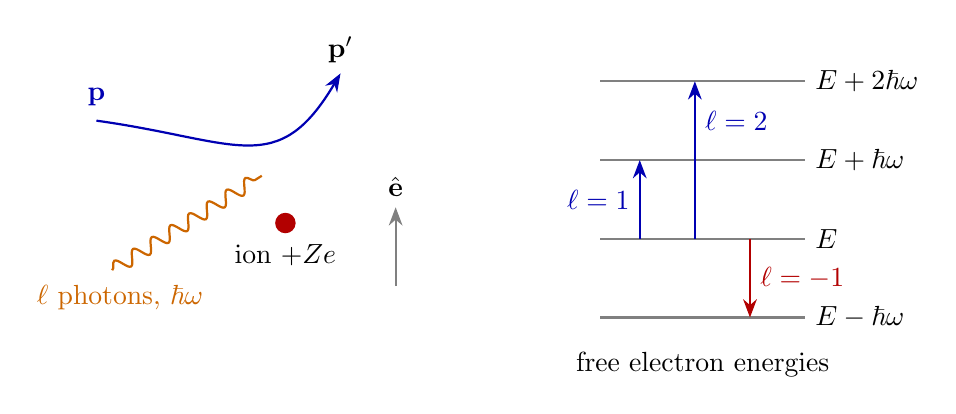
\begin{tikzpicture}[>=Stealth,thick]
\fill[red!70!black] (2.2,0) circle (0.13) node[below=4pt,black] {ion $+Ze$};
\draw[->,blue!70!black] (-0.2,1.3) .. controls (1.6,1.05) and (2.1,0.55) .. (2.9,1.9)
  node[above,black] {$\pv'$};
\node[blue!70!black] at (-0.2,1.6) {$\pv$};
\draw[decorate,decoration={snake,amplitude=2.5pt,segment length=8pt},orange!80!black]
  (0.0,-0.6) -- (1.9,0.6);
\node[orange!80!black] at (0.1,-0.95) {$\ell$ photons, $\hbar\omega$};
\draw[->,gray] (3.6,-0.8) -- (3.6,0.2) node[above,black] {$\ehat$};
\begin{scope}[xshift=6.2cm,yshift=-1.2cm]
\foreach \y/\lab in {0/{E-\hbar\omega},1/{E},2/{E+\hbar\omega},3/{E+2\hbar\omega}}{
  \draw[gray] (0,\y) -- (2.6,\y);
  \node[right] at (2.6,\y) {$\lab$};}
\draw[->,blue!70!black] (0.5,1) -- (0.5,2) node[pos=0.5,left] {$\ell=1$};
\draw[->,blue!70!black] (1.2,1) -- (1.2,3) node[pos=0.75,right] {$\ell=2$};
\draw[->,red!70!black] (1.9,1) -- (1.9,0) node[pos=0.5,right] {$\ell=-1$};
\node at (1.3,-0.6) {free electron energies};
\end{scope}
\end{tikzpicture}
\caption{Inverse bremsstrahlung. Left, an electron of momentum $\pv$
scatters on an ion into $\pv'$ while absorbing $\ell$ photons from the laser,
which is polarized along $\ehat$. The ion takes up the momentum
$\pv-\pv'$. Right, the energy of the free electron changes by $\ell\hbar\omega$,
with $\ell<0$ for stimulated emission.}
\label{pd:fig:process}
\end{figure}

\noindent\textbf{The plan of these notes.} Section~\ref{pd:sec:classical} sets out
the classical theory that the quantum theory must reproduce.
Section~\ref{pd:sec:hamiltonian} writes the Hamiltonian and the quiver motion.
Section~\ref{pd:sec:volkov} derives the Volkov states. Section~\ref{pd:sec:rates}
derives the multiphoton transition rates in Born approximation and the cross
section of Bunkin and Fedorov. Section~\ref{pd:sec:kinetic} derives the kinetic
equation for the occupation numbers with the operator method of the quantum
Boltzmann equation paper, and from it the heating rate.
Section~\ref{pd:sec:lindhard} writes the heating rate through the Lindhard
function. Section~\ref{pd:sec:closed} evaluates it in closed form for weak fields,
and Section~\ref{pd:sec:gaunt} connects it to the bremsstrahlung cross section,
the Gaunt factor and Kirchhoff's law. Section~\ref{pd:sec:manybody} derives the
same rate for the interacting electron gas and adds dynamic screening.
Section~\ref{pd:sec:strong} treats strong fields, and
Section~\ref{pd:sec:langdon} derives the kinetic equation of an isotropic
distribution and its Fokker--Planck limit. Section~\ref{pd:sec:summary} collects
the results. Appendix~\ref{pd:app:atzeni} reduces the results to the classical
treatment of Atzeni and Meyer-ter-Vehn equation by equation,
Appendix~\ref{pd:app:math} proves the mathematical identities, and
Appendix~\ref{pd:app:checks} lists the numerical checks.


\section{The classical baseline}
\label{pd:sec:classical}
\subsection{The Drude model}
\label{pd:sec:drude}
This subsection follows \cite[Sec.~11.1.1]{pd:Atzeni2004} and uses its
convention, in which a perturbation varies as $e^{i(\kv\cdot\rv-\omega t)}$ and
the physical quantity is the real part.

{\noindent}(1) The electron velocity obeys Newton's equation with a friction
force,
\begin{equation}
-i\omega m\vv=-e\Ev-\nu m\vv,
\label{pd:eq:drude-newton}
\end{equation}
which is Eq.~(11.7)~\cite{pd:Atzeni2004}. Collect the terms in $\vv$,
\begin{equation}
m(\nu-i\omega)\,\vv=-e\Ev
\quad\longrightarrow\quad
\vv=-\frac{e\Ev}{m(\nu-i\omega)}=-\frac{ie\Ev}{m(\omega+i\nu)},
\end{equation}
where the last step uses $\nu-i\omega=-i(\omega+i\nu)$ and $1/i=-i$.

{\noindent}(2) The current density and the conductivity are
\begin{equation}
\mathbf j=-en_e\vv=\frac{ie^2n_e}{m(\omega+i\nu)}\,\Ev,
\qquad
\sigma=\frac{ie^2n_e}{m(\omega+i\nu)}=\frac{e^2n_e}{m(\nu-i\omega)}.
\label{pd:eq:drude-sigma}
\end{equation}
Eq.~(11.8)~\cite{pd:Atzeni2004} prints $\mathbf j_1=e^2n_0\Ev_1/[im_e(\omega+i\nu_e)]$,
which is the negative of Eq.~\eqref{pd:eq:drude-sigma}. The sign of
Eq.~\eqref{pd:eq:drude-sigma} is the one that Eq.~(11.9)~\cite{pd:Atzeni2004}
requires, as the next step shows.

{\noindent}(3) With the dielectric tensor $\varepsilon=1+(4\pi i/\omega)\sigma$
of Eq.~(11.4)~\cite{pd:Atzeni2004},
\begin{equation}
\boxed{\;\varepsilon_T(\omega)=1+\frac{4\pi i}{\omega}\,\frac{ie^2n_e}{m(\omega+i\nu)}
=1-\frac{\omega_p^2}{\omega(\omega+i\nu)},\qquad
\omega_p^2=\frac{4\pi e^2n_e}{m},\;}
\label{pd:eq:drude-eps}
\end{equation}
which is Eq.~(11.9)~\cite{pd:Atzeni2004}. Its imaginary part is
\begin{equation}
\Imag\varepsilon_T=\frac{\omega_p^2}{\omega}\,\Imag\frac{-1}{\omega+i\nu}
=\frac{\omega_p^2}{\omega}\,\frac{\nu}{\omega^2+\nu^2}
=\frac{\omega_p^2\nu}{\omega^3}\Big[1+O\Big(\frac{\nu^2}{\omega^2}\Big)\Big].
\label{pd:eq:drude-imeps}
\end{equation}

{\noindent}(4) The power absorbed per unit volume is the cycle average of
$\mathbf j\cdot\Ev$. For the field $\Real[\Ev_1e^{-i\omega t}]$ with the real
amplitude $E_0=|\Ev_1|$,
\begin{equation}
\langle\mathbf j\cdot\Ev\rangle_t=\tfrac12\Real\sigma\,E_0^2
=\frac{\omega}{8\pi}\Imag\varepsilon_T\,E_0^2
=\frac{e^2n_e}{2m}\,\frac{\nu}{\nu^2+\omega^2}\,E_0^2.
\end{equation}
With the quiver velocity $v_0=eE_0/m\omega$ that Section~\ref{pd:sec:quiver}
derives,
\begin{equation}
\boxed{\;P=\frac{\omega}{8\pi}\Imag\varepsilon_T\,E_0^2
=n_e\,\nu\,\frac{mv_0^2}{2}\Big[1+O\Big(\frac{\nu^2}{\omega^2}\Big)\Big].\;}
\label{pd:eq:P-drude}
\end{equation}
The power is the collision rate times the kinetic energy $mv_0^2/2$ of the
quiver amplitude. Every quantum result of these notes is written in this form,
which defines the effective collision frequency
$\nueff\equiv P/(n_emv_0^2/2)$.

{\noindent}(5) The wave number of a transverse wave obeys
$k^2=(\omega^2/c^2)\varepsilon_T$, Eq.~(11.5)~\cite{pd:Atzeni2004}. To first order
in $\Imag\varepsilon_T$,
\begin{equation}
k=\frac{\omega}{c}\Big[(\Real\varepsilon_T)^{1/2}+\frac{i\Imag\varepsilon_T}{2(\Real\varepsilon_T)^{1/2}}\Big],
\end{equation}
and the intensity, which varies as $|E|^2\propto e^{-2\Imag k\,x}$, decays with
the coefficient
\begin{equation}
\boxed{\;K=2\Imag k=\frac{\omega}{c}\,\frac{\Imag\varepsilon_T}{(\Real\varepsilon_T)^{1/2}}
=\frac{\nueff}{c}\,\frac{\omega_p^2}{\omega^2}\,\frac{1}{n_r},
\qquad n_r=\Big(1-\frac{\omega_p^2}{\omega^2}\Big)^{1/2},\;}
\label{pd:eq:drude-K}
\end{equation}
which is Eq.~(11.12)~\cite{pd:Atzeni2004}. The same coefficient follows as the
ratio of $P$ to the energy flux $I=cn_rE_0^2/8\pi$ of the wave in the plasma.

\subsection{The collision frequency and the Coulomb logarithm}
\label{pd:sec:coulomblog}
{\noindent}(1) The electron collision time of
Eq.~(10.133)~\cite{pd:Atzeni2004} is
\begin{equation}
\frac1{\tau_e}=\frac{4\sqrt{2\pi}}{3}\,
\frac{n_iZ^2e^4}{m^{1/2}(\kB T)^{3/2}}\,\ln\Lambda_e
\equiv\nuT\ln\Lambda_e,\qquad
\boxed{\;\nuT=\frac{4\sqrt{2\pi}}{3}\,\frac{n_iZ^2e^4}{m^{1/2}(\kB T)^{3/2}}.\;}
\label{pd:eq:nuT}
\end{equation}
These notes write every collision frequency as $\nuT$ times a dimensionless
logarithm $\Lambda$, so that $\Lambda$ can be compared with $\ln\Lambda_e$
directly.

{\noindent}(2) The Coulomb logarithm of Eq.~(10.136)~\cite{pd:Atzeni2004} is
$\ln\Lambda_e=7.1-0.5\ln n_e+\ln T_e$ with $n_e$ in $10^{21}$~cm$^{-3}$ and
$T_e$ in keV. It is the logarithm of the ratio of the Debye length to the
de Broglie wavelength $\hbar/2mv$ at the velocity $mv^2/2=3\kB T/2$. The lower
cutoff is quantum mechanical, and the theory does not derive it.

{\noindent}(3) Two further points are not settled by the classical theory.
The collision time $\tau_e$ belongs to the slow relaxation of the electrons,
while the absorption of light at $\omega\gg\nu$ involves the collisions within
one period of the field. Dawson and Oberman \cite{pd:DawsonOberman1962} and
Johnston and Dawson \cite{pd:JohnstonDawson1973} showed that the upper cutoff is
then $v_t/\omega$ rather than the Debye length. The quantum theory produces
both cutoffs, Eq.~\eqref{pd:eq:Lambda-limits}.

\subsection{The free--free cross section}
\label{pd:sec:kramers}
{\noindent}(1) Kramers' cross section for the emission of a photon of
frequency $\nu$ by an electron of velocity $v$ in the field of an ion is
\cite{pd:Kramers1923}
\begin{equation}
\frac{\dd\sigma}{\dd\nu}=\frac{32\pi^2}{3\sqrt3}\,\frac{Z^2e^6}{m^2c^3v^2h\nu},
\label{pd:eq:kramers}
\end{equation}
Eq.~(10.89)~\cite{pd:Atzeni2004}. Quantum corrections are written as a Gaunt
factor $g$ that multiplies it.

{\noindent}(2) Averaged over a Maxwellian, Eq.~\eqref{pd:eq:kramers} gives the
emission coefficient of Eq.~(10.91)~\cite{pd:Atzeni2004}, and Kirchhoff's law
gives the free--free opacity of Eq.~(10.92)~\cite{pd:Atzeni2004}. Corrected for
stimulated emission and refraction, the absorption coefficient of the laser
light is Eq.~(11.34)~\cite{pd:Atzeni2004},
\begin{equation}
K=\rho\,\kappa^{\rm ff}_\nu\big(1-e^{-h\nu/\kB T_e}\big)\Big/\Big(1-\frac{\omega_p^2}{\omega_L^2}\Big)^{1/2}.
\label{pd:eq:atz-1134}
\end{equation}
Atzeni and Meyer-ter-Vehn state that this agrees with
Eq.~\eqref{pd:eq:drude-K} in its dependence on density, temperature and
wavelength, and in its numerical factor within a few percent. The dependences
agree, but with $g=1$ in Eq.~(10.92)~\cite{pd:Atzeni2004} and $\ln\Lambda_e=8$ the
numerical factors differ by a factor $4.4$. Section~\ref{pd:sec:gaunt} derives
the Gaunt factor that removes the difference, and
Appendix~\ref{pd:app:atzeni-ff} gives the numbers.

\medskip
\noindent\textbf{In Summary:} The classical theory takes three inputs. The
collision frequency enters the Drude model as a parameter, its Coulomb
logarithm needs a lower cutoff that is quantum mechanical, and the free--free
route needs a Gaunt factor. The quantum theory of the following sections
supplies all three, and its result is written as
$P=n_e\nueff\,mv_0^2/2$ with $\nueff=\nuT\Lambda$.

\section{The Hamiltonian}
\label{pd:sec:hamiltonian}
\subsection{The laser field and the quiver motion}
\label{pd:sec:quiver}
{\noindent}(1) The laser field is uniform over the region of a collision. Its
electric field and a vector potential that produces it, with zero scalar
potential, are
\begin{equation}
\Ev(t)=E_0\,\ehat\cos\omega t,\qquad
\Av(t)=-\frac{cE_0}{\omega}\,\ehat\sin\omega t,
\label{pd:eq:field}
\end{equation}
since $-c^{-1}\partial_t\Av=E_0\ehat\cos\omega t$. The validity of the
uniform field is the subject of Section~\ref{pd:sec:dipole}.

{\noindent}(2) A classical electron obeys $m\dot\vv=-eE_0\ehat\cos\omega t$.
Integrating once and twice,
\begin{equation}
\vv(t)=\vv_d-v_0\,\ehat\sin\omega t,\qquad
\rv(t)=\rv_d+\vv_dt+a_0\,\ehat\cos\omega t,
\end{equation}
where $\vv_d$ and $\rv_d$ are constants. The oscillating parts define the
quiver displacement and the quiver velocity,
\begin{equation}
\boxed{\;\begin{aligned}
&\boldsymbol\alpha(t)=\av\cos\omega t,\qquad
\vosc(t)=\dot{\boldsymbol\alpha}(t)=-v_0\,\ehat\sin\omega t,\qquad
\av=a_0\ehat,\\
&v_0=\frac{eE_0}{m\omega},\qquad a_0=\frac{v_0}{\omega}=\frac{eE_0}{m\omega^2},\qquad
\Up=\Big\langle\frac{m\vosc^2}{2}\Big\rangle_t=\frac{mv_0^2}{4}=\frac{e^2E_0^2}{4m\omega^2}.
\end{aligned}\;}
\label{pd:eq:quiver}
\end{equation}
Here $\langle\cdots\rangle_t$ is the average over one period, and $\Up$ is the
ponderomotive energy. The second derivative is
$\ddot{\boldsymbol\alpha}=-\omega^2\boldsymbol\alpha=-(e/m)\Ev(t)$, and the
quiver velocity is also
\begin{equation}
\dot{\boldsymbol\alpha}(t)=\frac{e}{mc}\Av(t).
\label{pd:eq:alpha-A}
\end{equation}

{\noindent}(3) For a charge $-e$ the canonical momentum is
$\pv=m\vv-(e/c)\Av$. With Eq.~\eqref{pd:eq:field}, $(e/c)\Av=-mv_0\ehat\sin\omega t$
and $\pv=m\vv+mv_0\ehat\sin\omega t=m\vv_d$ is constant. The canonical
momentum is the drift momentum, and the kinetic momentum
$m\vv=\pv+(e/c)\Av=\pv+m\vosc$ carries the quiver motion.

\subsection{The Hamiltonian of one electron}
{\noindent}(1) The Hamiltonian of one electron in the laser field and in the
field of the ions is
\begin{equation}
\boxed{\;H(t)=\frac{1}{2m}\Big[\hat\pv+\frac ec\Av(t)\Big]^2+V(\hat\rv),\qquad
V(\rv)=\sum_{j=1}^{N_i}v(\rv-\Rv_j),\;}
\label{pd:eq:H}
\end{equation}
where $v(\rv)$ is the potential energy of the electron in the field of one ion
and $N_i=n_i\Vol$.

{\noindent}(2) For a bare Coulomb ion $v(\rv)=-Ze^2/r$, and for a statically
screened one $v(\rv)=-Ze^2e^{-\kappa r}/r$. The Fourier transform follows from
the angular integral $\int e^{-i\kv\cdot\rv}\,\dd\Omega_r=4\pi\sin(kr)/kr$,
\begin{equation}
\int\frac{e^{-\kappa r}}{r}\,e^{-i\kv\cdot\rv}\,\dd^3r
=\frac{4\pi}{k}\int_0^\infty\sin(kr)\,e^{-\kappa r}\,\dd r
=\frac{4\pi}{k}\,\frac{k}{k^2+\kappa^2},
\end{equation}
so that
\begin{equation}
\boxed{\;\tilde v(\kv)=-\frac{4\pi Ze^2}{k^2+\kappa^2}
\;\xrightarrow{\;\kappa\to0\;}\;-\frac{4\pi Ze^2}{k^2}.\;}
\label{pd:eq:vk}
\end{equation}
These notes use the bare Coulomb form unless stated otherwise. Screening is
treated dynamically in Section~\ref{pd:sec:manybody}.

{\noindent}(3) With the Fourier series
$v(\rv)=\Vol^{-1}\sum_{\kv}\tilde v(\kv)e^{i\kv\cdot\rv}$ the potential of all
the ions is
\begin{equation}
V(\rv)=\frac{1}{\Vol}\sum_{\kv}\tilde v(\kv)\,\rho_i(\kv)\,e^{i\kv\cdot\rv},\qquad
\rho_i(\kv)=\sum_je^{-i\kv\cdot\Rv_j},\qquad
\tilde V(\kv)\equiv\int V(\rv)e^{-i\kv\cdot\rv}\dd^3r=\tilde v(\kv)\rho_i(\kv).
\label{pd:eq:Vk}
\end{equation}

\subsection{The oscillating frame of Kramers and Henneberger}
\label{pd:sec:KH1}
The quiver motion can be removed from the kinetic energy by going into the
frame that oscillates with the electron \cite{pd:Henneberger1968}. This frame
gives the clearest picture of inverse bremsstrahlung, and
Section~\ref{pd:sec:manybody} uses it for many electrons.

{\noindent}(1) Let $\hat T(t)=\exp[-(i/\hbar)\boldsymbol\alpha(t)\cdot\hat\pv]$,
which translates a wave function by $\boldsymbol\alpha$,
$(\hat T\phi)(\rv)=\phi(\rv-\boldsymbol\alpha)$. Then
$\hat T^\dagger V(\hat\rv)\hat T=V(\hat\rv+\boldsymbol\alpha)$, $\hat T$ commutes
with $\hat\pv$, and $i\hbar\,\partial_t\hat T=(\dot{\boldsymbol\alpha}\cdot\hat\pv)\hat T$,
because $\boldsymbol\alpha\cdot\hat\pv$ and $\dot{\boldsymbol\alpha}\cdot\hat\pv$
commute.

{\noindent}(2) Write the wave function as $\psi=e^{-iS(t)/\hbar}\hat T\phi$ with a
real function $S(t)$. Insert it into $i\hbar\partial_t\psi=H\psi$,
\begin{equation}
e^{-iS/\hbar}\hat T\big[\dot S+\dot{\boldsymbol\alpha}\cdot\hat\pv+i\hbar\partial_t\big]\phi
=e^{-iS/\hbar}\hat T\big[\hat T^\dagger H\hat T\big]\phi,
\end{equation}
and multiply by $e^{iS/\hbar}\hat T^\dagger$,
\begin{equation}
i\hbar\partial_t\phi=\Big[\frac{\hat p^2}{2m}+\frac{e}{mc}\Av\cdot\hat\pv+\frac{e^2A^2}{2mc^2}
+V(\hat\rv+\boldsymbol\alpha)-\dot{\boldsymbol\alpha}\cdot\hat\pv-\dot S\Big]\phi.
\end{equation}

{\noindent}(3) By Eq.~\eqref{pd:eq:alpha-A} the second and fifth terms cancel.
Choosing $\dot S=e^2A^2/2mc^2$ removes the third, which is independent of
position. What remains is
\begin{equation}
\boxed{\;i\hbar\partial_t\phi=\Big[\frac{\hat p^2}{2m}+V\big(\hat\rv+\boldsymbol\alpha(t)\big)\Big]\phi.\;}
\label{pd:eq:H-KH1}
\end{equation}
In this frame the electron is free and the ions oscillate. The ion $j$ sits at
$\Rv_j-\boldsymbol\alpha(t)$. A collision is elastic in the rest frame of the
ion, which is the laboratory, and the energy that the electron gains in the
oscillating frame comes from the motion of the ion relative to that frame.
Step~(3) of Section~\ref{pd:sec:classical-limit} makes this precise.

\subsection{Validity of the uniform field and of nonrelativistic motion}
\label{pd:sec:dipole}
The field of Eq.~\eqref{pd:eq:field} neglects the variation of the laser field
over the region of a collision and the magnetic force. Bunkin and Fedorov
state the conditions as $v/c\ll1$ and $\omega x_0/c\ll1$, where $x_0$ is the
larger of the distance $v/\omega$ traveled in one period and the quiver
amplitude $a_0$ \cite[Eq.~(4)]{pd:BunkinFedorov1966}. Since $\omega a_0=v_0$, both
conditions are $v\ll c$ and $v_0\ll c$, the nonrelativistic motion of the
electron. At $10^{15}$~W\,cm$^{-2}$ and $\lambda_L=0.351~\mu$m,
$v_0/c=0.0095$, and at 1~keV, $v_t/c=0.044$.


\section{The Volkov states}
\label{pd:sec:volkov}
\subsection{The solution}
{\noindent}(1) Without the ions the Schr\"odinger equation is
\begin{equation}
i\hbar\,\partial_t\psi=\frac{1}{2m}\Big[-i\hbar\nabla+\frac ec\Av(t)\Big]^2\psi.
\end{equation}
Since $\Av$ does not depend on position, the plane wave $e^{i\pv\cdot\rv/\hbar}$
is an eigenfunction of the operator on the right at every time. Try
$\psi=\Vol^{-1/2}e^{i\pv\cdot\rv/\hbar}e^{-i\Phi_{\pv}(t)}$, which gives
\begin{equation}
\hbar\dot\Phi_{\pv}=\frac{1}{2m}\Big[\pv+\frac ec\Av(t)\Big]^2.
\end{equation}

{\noindent}(2) Expand the square with Eq.~\eqref{pd:eq:field}, where
$(e/c)\Av=-mv_0\ehat\sin\omega t$,
\begin{equation}
\frac{1}{2m}\Big[\pv+\frac ec\Av\Big]^2=\frac{p^2}{2m}-v_0(\pv\cdot\ehat)\sin\omega t
+\frac{mv_0^2}{2}\sin^2\omega t
=E_{\pv}-v_0(\pv\cdot\ehat)\sin\omega t+\Up\,(1-\cos2\omega t),
\end{equation}
with $E_{\pv}=p^2/2m$ and $\Up=mv_0^2/4$. Integrate from $0$ to $t$ with
$\int_0^t\sin\omega t'\dd t'=(1-\cos\omega t)/\omega$ and
$\int_0^t\cos2\omega t'\dd t'=\sin(2\omega t)/2\omega$,
\begin{equation}
\hbar\Phi_{\pv}(t)=(E_{\pv}+\Up)\,t-\pv\cdot\av\,(1-\cos\omega t)-\frac{\Up}{2\omega}\sin2\omega t.
\end{equation}
The Volkov state is therefore \cite{pd:Volkov1935}
\begin{equation}
\boxed{\;\psi_{\pv}(\rv,t)=\frac{1}{\Vol^{1/2}}\exp\Big\{\frac{i}{\hbar}\Big[\pv\cdot\rv-(E_{\pv}+\Up)\,t
+\pv\cdot\av\,(1-\cos\omega t)+\frac{\Up}{2\omega}\sin2\omega t\Big]\Big\},\;}
\label{pd:eq:volkov}
\end{equation}
which is Eq.~(1)~\cite{pd:BunkinFedorov1966} with the integral in its phase
carried out for the field of Eq.~\eqref{pd:eq:field}, apart from the
normalization.

{\noindent}(3) The phase $\pv\cdot\rv+\pv\cdot\av(1-\cos\omega t)
=\pv\cdot[\rv-\boldsymbol\alpha(t)+\boldsymbol\alpha(0)]$ shows that the Volkov
wave is the plane wave of the oscillating frame of Section~\ref{pd:sec:KH1},
carried along with the quiver motion. The mean energy is $E_{\pv}+\Up$, and
$\Up$ is the same for all states, so it drops out of every energy
difference.

\subsection{Orthonormality and completeness}
At equal times the time-dependent phases are the same for the two factors of
a product with equal momenta, so
\begin{equation}
\int\psi^*_{\pv'}(\rv,t)\psi_{\pv}(\rv,t)\dd^3r=\delta_{\pv\pv'},\qquad
\sum_{\pv}\psi_{\pv}(\rv,t)\psi^*_{\pv}(\rv',t)=\frac1\Vol\sum_{\pv}e^{i\pv\cdot(\rv-\rv')/\hbar}=\delta(\rv-\rv').
\label{pd:eq:volkov-ortho}
\end{equation}
The Volkov states at time $t$ are a complete orthonormal set, and they can be
used as the basis of the many-electron field operator in
Section~\ref{pd:sec:kinetic}.

\subsection{The Jacobi--Anger expansion and three sum rules}
\label{pd:sec:bessel}
{\noindent}(1) The generating function of the Bessel functions is
$e^{\frac12z(\tau-\tau^{-1})}=\sum_{\ell}\tau^\ell J_\ell(z)$,
Eq.~(10.12.1)~\cite{pd:DLMF}. With $\tau=ie^{i\theta}$,
$\tau-\tau^{-1}=ie^{i\theta}+ie^{-i\theta}=2i\cos\theta$, and
\begin{equation}
\boxed{\;e^{iz\cos\theta}=\sum_{\ell=-\infty}^{\infty}i^\ell J_\ell(z)\,e^{i\ell\theta}.\;}
\label{pd:eq:jacobi-anger}
\end{equation}

{\noindent}(2) Parseval's theorem for the Fourier series in $\theta$ and for the
series of its derivative
$\partial_\theta e^{iz\cos\theta}=-iz\sin\theta\,e^{iz\cos\theta}=\sum_\ell i^\ell(i\ell)J_\ell e^{i\ell\theta}$
gives
\begin{equation}
\sum_\ell J_\ell^2(z)=\frac{1}{2\pi}\int_0^{2\pi}\big|e^{iz\cos\theta}\big|^2\dd\theta=1,\qquad
\sum_\ell\ell^2J_\ell^2(z)=\frac{1}{2\pi}\int_0^{2\pi}z^2\sin^2\theta\,\dd\theta=\frac{z^2}{2}.
\end{equation}
Since $J_{-\ell}=(-1)^\ell J_\ell$, the squares are even in $\ell$ and the
first moment vanishes. Altogether,
\begin{equation}
\boxed{\;\sum_\ell J_\ell^2(z)=1,\qquad\sum_\ell\ell\,J_\ell^2(z)=0,\qquad
\sum_\ell\ell^2J_\ell^2(z)=\frac{z^2}{2},\qquad J_{-\ell}^2=J_\ell^2.\;}
\label{pd:eq:bessel-sums}
\end{equation}

{\noindent}(3) For small arguments $J_\ell(z)=(\pm z/2)^{|\ell|}/|\ell|!+O(z^{|\ell|+2})$,
so that
\begin{equation}
J_0^2(z)=1-\frac{z^2}{2}+O(z^4),\qquad J_{\pm1}^2(z)=\frac{z^2}{4}+O(z^4),\qquad
J_{\pm\ell}^2(z)=O(z^{2|\ell|}).
\label{pd:eq:bessel-small}
\end{equation}

{\noindent}(4) Multiplying Eq.~\eqref{pd:eq:jacobi-anger} by the complex conjugate
of the same expansion at $\theta+s$ and averaging over $\theta$ gives the
generating function of the squares. With
$\cos\theta-\cos(\theta+s)=2\sin(s/2)\sin(\theta+s/2)$ and
$(2\pi)^{-1}\int_0^{2\pi}e^{ix\sin\varphi}\dd\varphi=J_0(x)$,
\begin{equation}
\boxed{\;\sum_\ell J_\ell^2(z)\,e^{-i\ell s}=\frac{1}{2\pi}\int_0^{2\pi}e^{iz[\cos\theta-\cos(\theta+s)]}\dd\theta
=J_0\Big(2z\sin\frac s2\Big).\;}
\label{pd:eq:bessel-genfun}
\end{equation}
This identity gives the classical limit in Section~\ref{pd:sec:classical-limit}.


\section{Multiphoton transition rates in Born approximation}
\label{pd:sec:rates}
\subsection{The transition amplitude}
{\noindent}(1) Expand the state of one electron in the Volkov states,
$\psi(t)=\sum_{\pv}c_{\pv}(t)\psi_{\pv}(t)$. Since each $\psi_{\pv}$ solves the
equation without ions, the Schr\"odinger equation with $H$ of
Eq.~\eqref{pd:eq:H} reduces to
\begin{equation}
i\hbar\,\dot c_{\pv'}=\sum_{\pv}V_{\pv'\pv}(t)\,c_{\pv},\qquad
V_{\pv'\pv}(t)=\int\psi^*_{\pv'}(\rv,t)V(\rv)\psi_{\pv}(\rv,t)\dd^3r.
\label{pd:eq:cdot}
\end{equation}
To first order in $V$, starting from $c_{\pv}(0)=\delta_{\pv\pv_i}$,
\begin{equation}
c_{\pv'}(t)=-\frac{i}{\hbar}\int_0^t V_{\pv'\pv_i}(t')\dd t'.
\label{pd:eq:c1}
\end{equation}

{\noindent}(2) In the matrix element the factor $\Vol^{-1}e^{-i(\pv'-\pv)\cdot\rv/\hbar}$
multiplies $V(\rv)$, and with $\hbar\kv=\pv'-\pv$ the spatial integral is
$\tilde V(\kv)/\Vol$ of Eq.~\eqref{pd:eq:Vk}. The time-dependent phases of
Eq.~\eqref{pd:eq:volkov} combine to
\begin{equation}
\begin{aligned}
\hbar(\Phi_{\pv'}-\Phi_{\pv})&=(E_{\pv'}-E_{\pv})\,t+\cancel{(\Up-\Up)\,t}
-(\pv'-\pv)\cdot\av\,(1-\cos\omega t)-\cancel{\Big(\frac{\Up}{2\omega}-\frac{\Up}{2\omega}\Big)\sin2\omega t}\\
&=(E_{\pv'}-E_{\pv})\,t-\hbar\kv\cdot\av\,(1-\cos\omega t),
\end{aligned}
\end{equation}
in which the terms with $\Up$ cancel because the ponderomotive energy is the
same for every state. With
$z\equiv\kv\cdot\av$ and Eq.~\eqref{pd:eq:jacobi-anger},
\begin{equation}
\boxed{\;V_{\pv'\pv}(t)=\frac{\tilde V(\kv)}{\Vol}\,e^{-iz}\sum_{\ell=-\infty}^{\infty}i^\ell J_\ell(z)\,
\exp\Big[\frac i\hbar\big(E_{\pv'}-E_{\pv}+\ell\hbar\omega\big)t\Big],\qquad
\hbar\kv=\pv'-\pv,\quad z=\kv\cdot\av.\;}
\label{pd:eq:Vpp}
\end{equation}
The matrix element is a sum of harmonics of the laser frequency, and the
$\ell$th harmonic carries the weight $J_\ell(z)$.

\subsection{The long-time limit}
{\noindent}(1) Insert Eq.~\eqref{pd:eq:Vpp} into Eq.~\eqref{pd:eq:c1},
\begin{equation}
c_{\pv'}(t)=-\frac{i}{\hbar}\,\frac{\tilde V(\kv)}{\Vol}\,e^{-iz}\sum_\ell i^\ell J_\ell(z)\,I_\ell(t),\qquad
I_\ell(t)=\int_0^te^{i\Omega_\ell t'}\dd t'=e^{i\Omega_\ell t/2}\,\frac{\sin(\Omega_\ell t/2)}{\Omega_\ell/2},
\end{equation}
with $\hbar\Omega_\ell=E_{\pv'}-E_{\pv}+\ell\hbar\omega$. The probability is
\begin{equation}
|c_{\pv'}(t)|^2=\frac{|\tilde V(\kv)|^2}{\hbar^2\Vol^2}\Big[\sum_\ell J_\ell^2(z)\,|I_\ell(t)|^2
+\sum_{\ell\neq\ell'}i^{\ell-\ell'}J_\ell(z)J_{\ell'}(z)\,I_\ell(t)I^*_{\ell'}(t)\Big].
\end{equation}

{\noindent}(2) The diagonal terms grow linearly in time. With
$x=\Omega t/2$, $\int\sin^2(\Omega t/2)/(\Omega/2)^2\,\dd\Omega
=2t\int\sin^2x/x^2\,\dd x=2\pi t$, and the function concentrates at $\Omega=0$
as $t$ grows, so that
\begin{equation}
|I_\ell(t)|^2=\frac{\sin^2(\Omega_\ell t/2)}{(\Omega_\ell/2)^2}\;\longrightarrow\;2\pi t\,\delta(\Omega_\ell)
=2\pi\hbar t\,\delta(\hbar\Omega_\ell).
\end{equation}

{\noindent}(3) The cross terms do not grow. The peaks of $|I_\ell|$ and
$|I_{\ell'}|$ sit at energies that differ by $(\ell-\ell')\hbar\omega$, so an
integral of $I_\ell I^*_{\ell'}$ over the final energies stays bounded as
$t\to\infty$. They describe the modulation of the scattering within a period
of the field, which produces harmonics of the current \cite{pd:Silin1965} and
averages out of the absorbed power.

{\noindent}(4) The transition rate $W=\dd|c_{\pv'}|^2/\dd t$ is then
\begin{equation}
W_{\pv\to\pv'}=\frac{2\pi}{\hbar}\,\frac{|\tilde V(\kv)|^2}{\Vol^2}\sum_\ell J_\ell^2(z)\,
\delta\big(E_{\pv'}-E_{\pv}+\ell\hbar\omega\big).
\end{equation}
Replacing $\ell$ by $-\ell$, which leaves $J_\ell^2$ unchanged by
Eq.~\eqref{pd:eq:bessel-sums}, puts it in the form in which $\ell>0$ counts
absorbed photons,
\begin{equation}
\boxed{\;W_{\pv\to\pv'}=\frac{2\pi}{\hbar}\,\frac{|\tilde V(\kv)|^2}{\Vol^2}\sum_{\ell=-\infty}^{\infty}
J_\ell^2(\kv\cdot\av)\,\delta\big(E_{\pv'}-E_{\pv}-\ell\hbar\omega\big),\qquad\hbar\kv=\pv'-\pv.\;}
\label{pd:eq:rate}
\end{equation}
The rate is symmetric, $W_{\pv\to\pv'}=W_{\pv'\to\pv}$, because the term
$\ell$ of one equals the term $-\ell$ of the other and $|\tilde V(-\kv)|=|\tilde V(\kv)|$.

\subsection{The average over the ion positions}
{\noindent}(1) By Eq.~\eqref{pd:eq:Vk},
$|\tilde V(\kv)|^2=|\tilde v(\kv)|^2|\rho_i(\kv)|^2$ with
\begin{equation}
|\rho_i(\kv)|^2=\sum_{j,j'}e^{-i\kv\cdot(\Rv_j-\Rv_{j'})}=N_i+\sum_{j\neq j'}e^{-i\kv\cdot(\Rv_j-\Rv_{j'})}.
\end{equation}

{\noindent}(2) For ions placed independently and uniformly in the box,
$\langle e^{-i\kv\cdot(\Rv_j-\Rv_{j'})}\rangle=|\langle e^{-i\kv\cdot\Rv}\rangle|^2=\delta_{\kv0}$
for $j\neq j'$, so $\langle|\rho_i(\kv)|^2\rangle=N_i$ for $\kv\neq0$. For
correlated ions the average defines the static structure factor,
$\langle|\rho_i(\kv)|^2\rangle=N_iS(\kv)$, and $S=1$ for independent ions.

{\noindent}(3) The averaged rate is
\begin{equation}
\boxed{\;W_{\pv\to\pv'}=\frac{2\pi}{\hbar}\,\frac{n_i}{\Vol}\,|\tilde v(\kv)|^2S(\kv)\sum_\ell
J_\ell^2(\kv\cdot\av)\,\delta\big(E_{\pv'}-E_{\pv}-\ell\hbar\omega\big).\;}
\label{pd:eq:rate-ions}
\end{equation}

\subsection{The cross section of Bunkin and Fedorov}
\label{pd:sec:bf}
{\noindent}(1) The rate of transitions of one electron into the final
directions $\dd\Omega'$ is the sum of Eq.~\eqref{pd:eq:rate-ions} over the final
states in that cone. With $\sum_{\pv'}\to\Vol\int p'^2\dd p'\,\dd\Omega'/(2\pi\hbar)^3$
and $\dd E_{\pv'}=p'\dd p'/m$, the energy delta function sets
$p'=p'_\ell\equiv(p^2+2m\ell\hbar\omega)^{1/2}$ and contributes $mp'_\ell$,
\begin{equation}
\dd\Gamma_\ell=\frac{2\pi}{\hbar}\,n_i|\tilde v(\kv)|^2S(\kv)J_\ell^2(\kv\cdot\av)\,
\frac{mp'_\ell}{(2\pi\hbar)^3}\,\dd\Omega'.
\end{equation}

{\noindent}(2) Dividing by the flux $n_iv=n_ip/m$ of ions seen by the electron
gives the cross section for the absorption of $\ell$ photons,
\begin{equation}
\boxed{\;\begin{aligned}
\frac{\dd\sigma_\ell}{\dd\Omega'}&=\frac{m^2}{4\pi^2\hbar^4}\,\frac{p'_\ell}{p}\,
|\tilde v(\kv)|^2S(\kv)\,J_\ell^2(\kv\cdot\av)
=\frac{p'_\ell}{p}\,J_\ell^2(\kv\cdot\av)\,\frac{\dd\sigma_B}{\dd\Omega}(\kv),\\
\frac{\dd\sigma_B}{\dd\Omega}&=\Big(\frac{m}{2\pi\hbar^2}\Big)^2|\tilde v(\kv)|^2S(\kv).
\end{aligned}\;}
\label{pd:eq:bf}
\end{equation}
Here $\dd\sigma_B/\dd\Omega$ is the field-free Born cross section at the
momentum transfer $\hbar\kv$. Equation~\eqref{pd:eq:bf} is
Eq.~(3)~\cite{pd:BunkinFedorov1966}, which normalizes the cross section by the
photon flux $I/\hbar\omega$ with $I=cE_0^2/8\pi$ and writes the argument of the
Bessel function as $\gamma[\cos\theta_0(1-\lambda\cos\theta)-\lambda\sin\theta_0\sin\theta\cos\varphi]$,
which is $-\kv\cdot\av$ in the present notation.

{\noindent}(3) For a bare Coulomb ion and $S=1$, with $\hbar k=2p\sin(\theta/2)$
for elastic scattering,
\begin{equation}
\frac{\dd\sigma_B}{\dd\Omega}=\frac{4m^2Z^2e^4}{\hbar^4k^4}=\Big(\frac{Ze^2}{2mv^2}\Big)^2\frac{1}{\sin^4(\theta/2)},
\label{pd:eq:rutherford}
\end{equation}
the Rutherford cross section. At $E_0=0$ only $\ell=0$ survives, with
$J_0(0)=1$, and Eq.~\eqref{pd:eq:bf} reduces to it.

{\noindent}(4) When $\ell\hbar\omega\ll E_{\pv}$ the factor $p'_\ell/p$ is close to
one, and the sum rule $\sum_\ell J_\ell^2=1$ shows that the field does not
change the total scattering. It distributes each scattering event over the
energies $E_{\pv}+\ell\hbar\omega$.

\subsection{Weak fields and one photon}
\label{pd:sec:onephoton}
{\noindent}(1) For $|\kv\cdot\av|\ll1$, Eq.~\eqref{pd:eq:bessel-small} keeps
$\ell=0,\pm1$. With Eq.~\eqref{pd:eq:vk} at $\kappa=0$ and $S=1$, the one-photon
cross sections are
\begin{equation}
\frac{\dd\sigma_{\pm1}}{\dd\Omega'}=\frac{m^2}{4\pi^2\hbar^4}\,\frac{p'_\pm}{p}\,
\frac{16\pi^2Z^2e^4}{k^4}\,\frac{(\kv\cdot\av)^2}{4}
=\frac{m^2Z^2e^4a_0^2}{\hbar^2}\,\frac{p'_\pm}{p}\,
\frac{[(\pv'-\pv)\cdot\ehat]^2}{|\pv'-\pv|^4},
\label{pd:eq:one-photon}
\end{equation}
with $p'_\pm=(p^2\pm2m\hbar\omega)^{1/2}$. The upper sign is absorption and the
lower one stimulated emission, which exists only for $E_{\pv}>\hbar\omega$.

{\noindent}(2) Let the incident momentum make the angle $\theta_0$ with
$\ehat$. Put $\pv$ along the $z$ axis, $\ehat=(\sin\theta_0,0,\cos\theta_0)$ and
$\pv'=p'(\sin\theta\cos\varphi,\sin\theta\sin\varphi,\cos\theta)$. The average
over $\varphi$ is
\begin{equation}
\big\langle[(\pv'-\pv)\cdot\ehat]^2\big\rangle_\varphi=\tfrac12p'^2\sin^2\theta\,\sin^2\theta_0
+(p'\cos\theta-p)^2\cos^2\theta_0.
\end{equation}
With $D=p^2+p'^2-2pp'c$, $c=\cos\theta$, the remaining integrals are
elementary. Using $b=2pp'$, $a=p^2+p'^2$, $\Delta=p^2-p'^2$ and
$L=\ln[(p+p')/|p-p'|]$,
\begin{equation}
\int_{-1}^1\frac{\dd c}{D^2}=\frac{2}{\Delta^2},\qquad
\int_{-1}^1\frac{c\,\dd c}{D^2}=\frac{2a}{b\Delta^2}-\frac{2L}{b^2},\qquad
\int_{-1}^1\frac{c^2\dd c}{D^2}=\frac{2a^2}{b^2\Delta^2}-\frac{4aL}{b^3}+\frac{2}{b^2},
\end{equation}
from which, using $b^2-a^2=-\Delta^2$ and $(a-2p^2)^2=\Delta^2$,
\begin{equation}
\int_{-1}^1\frac{(1-c^2)\,\dd c}{D^2}=\frac{(p^2+p'^2)L}{2p^3p'^3}-\frac{1}{p^2p'^2},\qquad
\int_{-1}^1\frac{(p'c-p)^2\dd c}{D^2}=\frac{1}{p^2}+\frac{(p^2-p'^2)L}{2p^3p'}.
\end{equation}

{\noindent}(3) Collecting,
\begin{equation}
\boxed{\;\sigma_{\pm1}(\theta_0)=\frac{2\pi m^2Z^2e^4a_0^2}{\hbar^2p^2}\,\frac{p'_\pm}{p}
\Big\{\sin^2\theta_0\Big[\frac{(p^2+p'^2_\pm)L_\pm}{4pp'_\pm}-\frac12\Big]
+\cos^2\theta_0\Big[1+\frac{(p^2-p'^2_\pm)L_\pm}{2pp'_\pm}\Big]\Big\},\;}
\label{pd:eq:sigma-theta0}
\end{equation}
with $L_\pm=\ln[(p+p'_\pm)/|p-p'_\pm|]$.

{\noindent}(4) The average over the orientation of $\pv$ uses
$\langle\sin^2\theta_0\rangle=2/3$ and $\langle\cos^2\theta_0\rangle=1/3$. The
terms without $L$ cancel and
\begin{equation}
\boxed{\;\bar\sigma_{\pm1}(p)=\frac{2\pi}{3}\,\frac{m^2Z^2e^4a_0^2}{\hbar^2p^2}\,L_\pm,\qquad
L_\pm=\ln\frac{p+p'_\pm}{|p-p'_\pm|}.\;}
\label{pd:eq:sigma-iso}
\end{equation}

{\noindent}(5) Bunkin and Fedorov expand Eq.~\eqref{pd:eq:sigma-theta0} for
$\xi=\hbar\omega/mv^2\ll1$, in their normalization per photon flux.
Multiplying by $n_iv\hbar\omega/I$ with $I=cE_0^2/8\pi$ and
$a_0^2=e^2E_0^2/m^2\omega^4$ turns the prefactor of
Eq.~\eqref{pd:eq:sigma-theta0} into $16\pi^2n_iZ^2e^6/(m^2vc\hbar\omega^3)$. With
$p'_\pm=p(1\pm2\xi)^{1/2}$, $L_\pm=\ln(2/\xi)\pm\xi+O(\xi^2)$ and the curly
bracket to first order in $\xi$, the result is
\begin{equation}
\sigma^{\rm BF}_{a,e}=\frac{8\pi^2Z^2e^6n_i}{m^2vc\hbar\omega^3}\Big[(3\cos^2\theta_0-1)
+(1-\cos^2\theta_0)\ln\frac2\xi\mp(3\cos^2\theta_0-1)\,\xi\ln\frac2\xi\pm2\xi\cos^2\theta_0\Big],
\label{pd:eq:bf10}
\end{equation}
which is Eq.~(10)~\cite{pd:BunkinFedorov1966} term by term, with the upper sign for
absorption. The net emission $\sigma_e-\sigma_a$ is proportional to
$(3\cos^2\theta_0-1)\ln(2/\xi)-2\cos^2\theta_0$. It is positive for electrons
moving along the field, which then amplify it, as Marcuse first found
\cite{pd:Marcuse1962}. Averaged over directions it is $-2/3$ times the
prefactor, and the plasma absorbs.

\subsection{The classical limit of the photon-number distribution}
\label{pd:sec:classical-limit}
{\noindent}(1) Let $\hbar\omega\to0$ at a fixed quiver velocity, so that
$z=\kv\cdot\av\to\infty$ while $Z_E\equiv z\hbar\omega=\hbar\kv\cdot\ehat\,v_0$
stays fixed. Take a smooth test function $\phi(\epsilon)$ of the energy
transfer with Fourier representation $\phi(\epsilon)=\int\hat\phi(\tau)e^{-i\epsilon\tau}\dd\tau$.
By Eq.~\eqref{pd:eq:bessel-genfun} with $s=\hbar\omega\tau$,
\begin{equation}
\sum_\ell J_\ell^2(z)\,\phi(\ell\hbar\omega)=\int\hat\phi(\tau)\,J_0\Big(2z\sin\frac{\hbar\omega\tau}{2}\Big)\dd\tau
\;\longrightarrow\;\int\hat\phi(\tau)\,J_0(Z_E\tau)\,\dd\tau.
\end{equation}

{\noindent}(2) With $J_0(x)=(2\pi)^{-1}\int_0^{2\pi}e^{-ix\cos\theta}\dd\theta$
the limit is $(2\pi)^{-1}\int_0^{2\pi}\phi(Z_E\cos\theta)\,\dd\theta$. In
distributional form,
\begin{equation}
\boxed{\;\sum_\ell J_\ell^2(z)\,\delta(\epsilon-\ell\hbar\omega)\;\longrightarrow\;
\frac{1}{2\pi}\int_0^{2\pi}\delta(\epsilon-Z_E\cos\theta)\,\dd\theta
=\frac{1}{\pi}\,\frac{\Theta(Z_E^2-\epsilon^2)}{(Z_E^2-\epsilon^2)^{1/2}},\qquad
Z_E=\hbar|\kv\cdot\ehat|\,v_0.\;}
\label{pd:eq:arcsine}
\end{equation}

{\noindent}(3) This is the classical picture. The ion is at rest in the
laboratory, so a collision that is short compared with the period conserves
the kinetic energy $m|\vv|^2/2$ of the electron while its momentum changes by
$\hbar\kv$. The kinetic momentum is $m\vv=\pv+m\vosc$, so the drift energy
$E_{\pv}=|m\vv-m\vosc|^2/2m$ changes by
$\Delta\epsilon=-\hbar\kv\cdot\vosc(t_c)=\hbar(\kv\cdot\ehat)v_0\sin\omega t_c$,
where $t_c$ is the time of the collision. A uniformly distributed phase
$\omega t_c$ gives the arcsine density of Eq.~\eqref{pd:eq:arcsine}.

\medskip
\noindent\textbf{Remarks:}\\
(1) The Born approximation for a Coulomb ion needs $\eta=Ze^2/\hbar v\ll1$,
Eq.~(5)~\cite{pd:BunkinFedorov1966}. Since $\eta=r_0/\lambdabar$ with
$r_0=Ze^2/mv^2$ and $\lambdabar=\hbar/mv$, it is the condition that the
de Broglie wavelength exceeds the distance of closest approach. It is the
same condition that selects the quantum lower cutoff of the Coulomb logarithm
in \cite[Eq.~(10.136)]{pd:Atzeni2004} and the Bethe rather than the Bohr
stopping number in \cite[Eq.~(11.74)]{pd:Atzeni2004}. At the thermal velocity
$\eta=Z(2\,{\rm Ry}/\kB T)^{1/2}$, with $2\,{\rm Ry}=27.2$~eV.\\
(2) At first order in $E_0$ the amplitude of Eq.~\eqref{pd:eq:Vpp} with $\ell=1$
is that of second-order perturbation theory, with one photon vertex
$(e/mc)\Av\cdot\hat\pv$ and one ion vertex in both orders. The photon vertex
is diagonal in momentum, so the two orders have the intermediate states
$\pv$ and $\pv'$, the energy denominators $\hbar\omega$ and $-\hbar\omega$, and the
amplitude $(e/mc\hbar\omega)\Av_1\cdot(\pv-\pv')\tilde V(\kv)/\Vol$, where
$\Av_1$ is the amplitude of $e^{-i\omega t}$ in $\Av$, of magnitude $cE_0/2\omega$.
Its magnitude is $\tfrac12|\kv\cdot\av||\tilde V|/\Vol$, which is
$J_1(\kv\cdot\av)|\tilde V|/\Vol$ to this order. The term
$e^2A^2/2mc^2$ only shifts all energies by $\Up$ and does not contribute.\\
(3) The weak-field cross sections of Eq.~\eqref{pd:eq:sigma-iso} are what the
kinetic equation of Section~\ref{pd:sec:langdon} needs for an isotropic
distribution.

\section{The kinetic equation}
\label{pd:sec:kinetic}
This section derives the equation of motion of the occupation numbers with
the operator method that Section~2 of the quantum Boltzmann equation paper
\cite{pd:Watson2026} uses for a quartic interaction. The electrons are taken as
independent here. Their interaction enters in Section~\ref{pd:sec:manybody}.

\subsection{The field operator in the Volkov basis}
{\noindent}(1) Expand the electron field operator of spin $\sigma$ in the
Volkov states, which are complete at every time by
Eq.~\eqref{pd:eq:volkov-ortho},
\begin{equation}
\hat\Psi_\sigma(\rv,t)=\sum_{\pv}\psi_{\pv}(\rv,t)\,\hat b_{\pv\sigma},\qquad
\hat b_{\pv\sigma}\hat b^\dagger_{\pv'\sigma'}-\eta_s\,\hat b^\dagger_{\pv'\sigma'}\hat b_{\pv\sigma}
=\delta_{\pv\pv'}\delta_{\sigma\sigma'},
\end{equation}
with $\eta_s=-1$ for electrons. The value $\eta_s=+1$ for bosons is kept to
show that the result does not depend on it.

{\noindent}(2) In the interaction picture with respect to the motion in the
laser field, the time dependence of the free motion is carried by the mode
functions $\psi_{\pv}$, the operators $\hat b_{\pv\sigma}$ are constant in
the absence of ions, and the ion potential is the one-body operator
\begin{equation}
\hat H_V(t)=\sum_\sigma\int\hat\Psi^\dagger_\sigma V\hat\Psi_\sigma\,\dd^3r
=\sum_\sigma\sum_{\pv,\pv'}V_{\pv'\pv}(t)\,\hat b^\dagger_{\pv'\sigma}\hat b_{\pv\sigma},
\label{pd:eq:HV}
\end{equation}
with the matrix elements of Eq.~\eqref{pd:eq:Vpp}. The potential does not act
on the spin, and the spin label is dropped from here on.

\subsection{The exact equation of motion of the one-body density matrix}
{\noindent}(1) The commutator of two bilinears is the same for both
statistics. For fermions,
\begin{equation}
\hat b^\dagger_a\hat b_b\hat b^\dagger_c\hat b_d
=\delta_{bc}\hat b^\dagger_a\hat b_d-\hat b^\dagger_a\hat b^\dagger_c\hat b_b\hat b_d,\qquad
\hat b^\dagger_c\hat b_d\hat b^\dagger_a\hat b_b
=\delta_{ad}\hat b^\dagger_c\hat b_b-\hat b^\dagger_c\hat b^\dagger_a\hat b_d\hat b_b,
\end{equation}
and the quartic terms are equal because
$\hat b^\dagger_c\hat b^\dagger_a\hat b_d\hat b_b=(-\hat b^\dagger_a\hat b^\dagger_c)(-\hat b_b\hat b_d)$.
For bosons both signs change and the quartic terms are again equal. Hence
\begin{equation}
\big[\hat b^\dagger_a\hat b_b,\hat b^\dagger_c\hat b_d\big]=\delta_{bc}\,\hat b^\dagger_a\hat b_d-\delta_{ad}\,\hat b^\dagger_c\hat b_b.
\label{pd:eq:bilinear}
\end{equation}

{\noindent}(2) The Heisenberg equation for $\hat b^\dagger_k\hat b_{k'}$, with
$k,k'$ short for momenta, is then
\begin{equation}
\frac{\dd}{\dd t}\big(\hat b^\dagger_k\hat b_{k'}\big)=\frac i\hbar\big[\hat H_V,\hat b^\dagger_k\hat b_{k'}\big]
=\frac i\hbar\sum_{c,d}V_{cd}\big(\delta_{dk}\hat b^\dagger_c\hat b_{k'}-\delta_{ck'}\hat b^\dagger_k\hat b_d\big)
=\frac i\hbar\sum_c\big(V_{ck}\,\hat b^\dagger_c\hat b_{k'}-V_{k'c}\,\hat b^\dagger_k\hat b_c\big).
\end{equation}
With the one-body density matrix $\rho_{ab}=\langle\hat b^\dagger_a\hat b_b\rangle$,
\begin{equation}
\boxed{\;\frac{\dd\rho_{kk'}}{\dd t}=\frac i\hbar\sum_c\big[V_{ck}(t)\,\rho_{ck'}-V_{k'c}(t)\,\rho_{kc}\big].\;}
\label{pd:eq:eom}
\end{equation}

{\noindent}(3) Equation~\eqref{pd:eq:eom} is exact and closed. In the quantum
Boltzmann equation paper the quartic interaction makes the right side of
Eq.~(4)~\cite{pd:Watson2026} a product of four operators, whose average at second
order needs the six-field correlator and Wick's theorem. Here the ion
potential is a one-body operator, the right side is again bilinear, and no
factorization is needed.

\subsection{Second order and the Markov limit}
{\noindent}(1) Let the initial state be homogeneous, $\rho_{ab}(0)=\delta_{ab}f_a$.
To first order in $V$, Eq.~\eqref{pd:eq:eom} has $\sum_cV_{ca}\rho_{cb}=V_{ba}f_b$
and $\sum_cV_{bc}\rho_{ac}=V_{ba}f_a$, so
\begin{equation}
\rho^{(1)}_{ab}(t)=\frac i\hbar\,(f_b-f_a)\int_0^tV_{ba}(t')\,\dd t'.
\label{pd:eq:rho1}
\end{equation}
The diagonal elements do not change at first order, because
$f_k-f_k=0$. This is the vanishing of the mean-field term that the quantum
Boltzmann equation paper finds for $\mathbf k=\mathbf k'$ in its Eq.~(5)~\cite{pd:Watson2026}.

{\noindent}(2) For the diagonal element at second order, insert
Eq.~\eqref{pd:eq:rho1} into Eq.~\eqref{pd:eq:eom} with $k'=k$. Since
$\rho^{(1)}_{kc}=\rho^{(1)*}_{ck}$ and $V_{kc}=V^*_{ck}$, the two terms are
$\zeta_c-\zeta^*_c=2i\Imag\zeta_c$ with
$\zeta_c=V_{ck}(t)\rho^{(1)}_{ck}(t)=(i/\hbar)(f_k-f_c)V_{ck}(t)\int_0^tV_{kc}(t')\dd t'$, and
\begin{equation}
\frac{\dd f_k}{\dd t}=-\frac2\hbar\sum_c\Imag\zeta_c
=\frac{2}{\hbar^2}\sum_c\,(f_c-f_k)\,\Real\Big[V^*_{kc}(t)\int_0^tV_{kc}(t')\,\dd t'\Big].
\label{pd:eq:second-order}
\end{equation}
Since $\Real[V^*(t)\int_0^tV\dd t']=\tfrac12\dd|\int_0^tV\dd t'|^2/\dd t$, the
bracket is $\hbar^2/2$ times the rate of growth of the transition probability of
Eq.~\eqref{pd:eq:c1}.

{\noindent}(3) Insert Eq.~\eqref{pd:eq:Vpp}. The phases $e^{-iz}$ cancel between
$V^*_{kc}$ and $V_{kc}$, and with $\hbar\Omega_\ell=E_k-E_c+\ell\hbar\omega$ and
$\tau=t-t'$,
\begin{equation}
\Real\Big[V^*_{kc}(t)\int_0^tV_{kc}(t')\dd t'\Big]
=\frac{|\tilde V|^2}{\Vol^2}\sum_{\ell,\ell'}\Real\Big[i^{\ell'-\ell}J_\ell J_{\ell'}\,
e^{i(\ell'-\ell)\omega t}\int_0^te^{-i\Omega_{\ell'}\tau}\dd\tau\Big].
\end{equation}
The terms with $\ell'\neq\ell$ oscillate at multiples of $\omega$ and average to
zero over a period. The terms with $\ell'=\ell$ contain
\begin{equation}
\Real\int_0^te^{-i\Omega\tau}\dd\tau=\frac{\sin\Omega t}{\Omega}\;\longrightarrow\;\pi\,\delta(\Omega)\qquad(t\to\infty).
\label{pd:eq:markov}
\end{equation}
The one-sided time integral gives $\pi\delta$, and the factor $2$ of
Eq.~\eqref{pd:eq:second-order}, which comes from the two Hermitian-conjugate
terms, completes the $2\pi$ of the golden rule. This is the step at which the
published Eqs.~(5)--(7)~\cite{pd:Watson2026} carry twice the coefficient, as the
erratum \cite{pd:Watson2026erratum} corrects.

{\noindent}(4) With $\delta(\Omega)=\hbar\,\delta(\hbar\Omega)$ the result is
$\dd f_k/\dd t=\sum_cW_{c\to k}(f_c-f_k)$ with the rate of
Eq.~\eqref{pd:eq:rate}, and after the average over the ion positions with the
rate of Eq.~\eqref{pd:eq:rate-ions},
\begin{equation}
\boxed{\;\frac{\partial f_{\pv}}{\partial t}=\sum_{\pv'}W_{\pv'\to\pv}\,\big(f_{\pv'}-f_{\pv}\big),\qquad
W_{\pv'\to\pv}=W_{\pv\to\pv'}.\;}
\label{pd:eq:master}
\end{equation}
This is the kinetic equation of inverse bremsstrahlung, a master equation in
which each pair of states is connected by the multiphoton rates of
Bunkin and Fedorov.

\subsection{Why there is no Pauli blocking}
\label{pd:sec:blocking}
The Uehling--Uhlenbeck form of the collision integral,
Eq.~(7)~\cite{pd:Watson2026}, carries the factors $1+\eta_sn$ of the final
states. For scattering on a static potential the gain and the loss term of one
pair of states combine as
\begin{equation}
f_{\pv'}(1+\eta_sf_{\pv})-f_{\pv}(1+\eta_sf_{\pv'})=f_{\pv'}-f_{\pv},
\label{pd:eq:no-blocking}
\end{equation}
because the quadratic terms are equal. The exact one-body equation of
motion never produced them. Pauli blocking does not suppress inverse
bremsstrahlung on static ions, but the Fermi--Dirac distribution enters
through $f$ itself, Section~\ref{pd:sec:degenerate}.

\subsection{Conservation, equilibrium and the heating rate}
{\noindent}(1) Summing Eq.~\eqref{pd:eq:master} over $\pv$ and using the
symmetry of $W$ shows that the number of electrons is conserved. Momentum is
not conserved, because the ions absorb it.

{\noindent}(2) Without the field only $\ell=0$ survives, $W$ contains
$\delta(E_{\pv'}-E_{\pv})$, and every distribution that depends on the energy
alone is stationary. The field drives the electrons through the terms with
$\ell\neq0$.

{\noindent}(3) The kinetic energy of the drift motion per unit volume,
counting both spin states, is $u_e=(2/\Vol)\sum_{\pv}E_{\pv}f_{\pv}$. The
quiver energy $\Up$ per electron is constant and absorbs nothing on average.
With Eq.~\eqref{pd:eq:master}, and then with the labels $\pv,\pv'$ exchanged and
the two forms averaged,
\begin{equation}
P=\frac{\dd u_e}{\dd t}=\frac2\Vol\sum_{\pv,\pv'}E_{\pv}W_{\pv'\to\pv}(f_{\pv'}-f_{\pv})
=\frac1\Vol\sum_{\pv,\pv'}\big(E_{\pv}-E_{\pv'}\big)W_{\pv'\to\pv}(f_{\pv'}-f_{\pv}).
\end{equation}

{\noindent}(4) The term $\ell$ of the rate fixes $E_{\pv}-E_{\pv'}=\ell\hbar\omega$.
Pairing the term $-\ell$ with the term $\ell$ after exchanging $\pv$ and $\pv'$
in it, which uses $J^2_{-\ell}=J^2_\ell$, gives
\begin{equation}
\boxed{\;\begin{aligned}
P&=\frac2\Vol\sum_{\ell=1}^\infty\ell\hbar\omega\sum_{\pv,\pv'}w_\ell(\pv'\to\pv)\,
\big(f_{\pv'}-f_{\pv}\big),\\
w_\ell(\pv'\to\pv)&=\frac{2\pi}{\hbar}\frac{n_i}{\Vol}|\tilde v(\kv)|^2S(\kv)J_\ell^2(\kv\cdot\av)\,
\delta(E_{\pv}-E_{\pv'}-\ell\hbar\omega),
\end{aligned}\;}
\label{pd:eq:P-general}
\end{equation}
with $\hbar\kv=\pv-\pv'$. Each term is a transition from the lower energy
$E_{\pv'}$ to the higher one $E_{\pv}=E_{\pv'}+\ell\hbar\omega$, absorption
minus stimulated emission.

{\noindent}(5) If $f$ is a decreasing function of the energy alone, every
difference $f_{\pv'}-f_{\pv}$ is positive and $P\geq0$. Free--free gain needs
either an inverted energy distribution or an anisotropic one, as for the
electrons moving along the field in Eq.~\eqref{pd:eq:bf10}.

\medskip
\noindent\textbf{In Summary:} The occupation numbers obey the master
equation~\eqref{pd:eq:master}, derived exactly from the operator equation of
motion to second order in the ion potential. No Pauli blocking appears, and the
heating rate is Eq.~\eqref{pd:eq:P-general}.


\section{The heating rate and the Lindhard function}
\label{pd:sec:lindhard}
\subsection{The heating rate through the Lindhard function}
{\noindent}(1) In Eq.~\eqref{pd:eq:P-general} write the initial momentum as
$\mathbf q$ and the final one as $\mathbf q+\hbar\kv$, with
$\sum_{\mathbf q}\to\Vol\int\dd^3q/(2\pi\hbar)^3$ and
$\sum_{\kv}\to\Vol\int\dd^3k/(2\pi)^3$,
\begin{equation}
P=\sum_{\ell=1}^\infty\ell\hbar\omega\,\frac{2\pi}{\hbar}\,n_i\int\frac{\dd^3k}{(2\pi)^3}\,|\tilde v(\kv)|^2S(\kv)J_\ell^2(\kv\cdot\av)
\Big\{2\int\frac{\dd^3q}{(2\pi\hbar)^3}\,\delta\big(E_{\mathbf q+\hbar\kv}-E_{\mathbf q}-\ell\hbar\omega\big)
\big(f_{\mathbf q}-f_{\mathbf q+\hbar\kv}\big)\Big\}.
\end{equation}

{\noindent}(2) The density response function of free electrons, the Lindhard
function \cite{pd:Lindhard1954}, is
\begin{equation}
\boxed{\;\chi_0(\kv,\Omega)=2\int\frac{\dd^3q}{(2\pi\hbar)^3}\,
\frac{f_{\mathbf q}-f_{\mathbf q+\hbar\kv}}{\hbar\Omega+E_{\mathbf q}-E_{\mathbf q+\hbar\kv}+i0^+},\;}
\label{pd:eq:chi0}
\end{equation}
the factor $2$ counting the spin. With $\Imag(x+i0^+)^{-1}=-\pi\delta(x)$ the
curly bracket is $-\Imag\chi_0(\kv,\ell\omega)/\pi$, and
\begin{equation}
P=-2n_i\sum_{\ell=1}^\infty\ell\omega\int\frac{\dd^3k}{(2\pi)^3}\,|\tilde v(\kv)|^2S(\kv)J_\ell^2(\kv\cdot\av)\,
\Imag\chi_0(\kv,\ell\omega).
\end{equation}

{\noindent}(3) Changing $\mathbf q\to\mathbf q+\hbar\kv$ in Eq.~\eqref{pd:eq:chi0}
shows $\chi_0(-\kv,-\Omega)^*=\chi_0(\kv,\Omega)$, so
$\Imag\chi_0(-\kv,-\Omega)=-\Imag\chi_0(\kv,\Omega)$. Since the rest of the
integrand is even in $\kv$, the term $-\ell$ equals the term $\ell$, and the sum
can run over all $\ell$,
\begin{equation}
\boxed{\;P=-n_i\sum_{\ell=-\infty}^{\infty}\ell\omega\int\frac{\dd^3k}{(2\pi)^3}\,|\tilde v(\kv)|^2S(\kv)\,
J_\ell^2(\kv\cdot\av)\,\Imag\chi_0(\kv,\ell\omega).\;}
\label{pd:eq:P-chi0}
\end{equation}
This form holds for any distribution $f$, isotropic or not, and any field
strength. Section~\ref{pd:sec:manybody} shows that the interacting electron gas
gives the same formula with $\chi_0$ replaced by its density response.

\subsection{The imaginary part of the Lindhard function}
\label{pd:sec:imchi}
{\noindent}(1) For an isotropic distribution $f_{\mathbf q}=f(E_{\mathbf q})$,
write $\Imag\chi_0=-2\pi\int\dd^3q\,(2\pi\hbar)^{-3}[f(E_{\mathbf q})-f(E_{\mathbf q+\hbar\kv})]
\,\delta(\hbar\Omega+E_{\mathbf q}-E_{\mathbf q+\hbar\kv})$. In the first term
$E_{\mathbf q+\hbar\kv}-E_{\mathbf q}=\hbar kq_\parallel/m+\hbar^2k^2/2m$ with
$q_\parallel=\mathbf q\cdot\hat\kv$, so the delta function is
$(m/\hbar k)\,\delta(q_\parallel-mc_-)$ with $c_-=\Omega/k-\hbar k/2m$.

{\noindent}(2) The integral over the transverse momentum is
$\int f\,\dd^2q_\perp=\pi\int f\,\dd(q_\perp^2)=2\pi m\int_{E_-}^\infty f(E)\,\dd E$,
where $E_-=mc_-^2/2$ is the energy at $q_\perp=0$.

{\noindent}(3) In the second term the shift $\mathbf q\to\mathbf q-\hbar\kv$
turns the condition into $\hbar kq_\parallel/m-\hbar^2k^2/2m=\hbar\Omega$, that
is $q_\parallel=mc_+$ with $c_+=\Omega/k+\hbar k/2m$ and $E_+=mc_+^2/2$.

{\noindent}(4) Subtracting the two and collecting the constants
$2\pi\cdot2\pi m\cdot m/[(2\pi\hbar)^3\hbar k]=m^2/2\pi\hbar^4k$,
\begin{equation}
\boxed{\;\Imag\chi_0(\kv,\Omega)=-\frac{m^2}{2\pi\hbar^4k}\int_{E_-}^{E_+}f(E)\,\dd E,\qquad
E_\pm=\frac m2\Big(\frac\Omega k\pm\frac{\hbar k}{2m}\Big)^2.\;}
\label{pd:eq:imchi-general}
\end{equation}
For $\Omega>0$, $E_+>E_-$ and $\Imag\chi_0<0$.

{\noindent}(5) For the Fermi--Dirac distribution
$f=[e^{(E-\mu)/\kB T}+1]^{-1}$, with the antiderivative
$-\kB T\ln(1+e^{(\mu-E)/\kB T})$,
\begin{equation}
\boxed{\;\Imag\chi_0(\kv,\Omega)=-\frac{m^2\kB T}{2\pi\hbar^4k}\,
\ln\frac{1+e^{(\mu-E_-)/\kB T}}{1+e^{(\mu-E_+)/\kB T}}.\;}
\label{pd:eq:imchi-fd}
\end{equation}

{\noindent}(6) For nondegenerate electrons $f=e^{(\mu-E)/\kB T}$ with
$e^{\mu/\kB T}=\frac12n_e(2\pi\hbar^2/m\kB T)^{3/2}$, and the constants
combine into $(\pi/2)^{1/2}/\hbar kv_t$,
\begin{equation}
\boxed{\;\Imag\chi_0(\kv,\Omega)=-n_e\Big(\frac\pi2\Big)^{1/2}\frac{1}{\hbar kv_t}
\Big[e^{-E_-/\kB T}-e^{-E_+/\kB T}\Big],\qquad
\frac{E_\pm}{\kB T}=\frac12\Big(\frac{\Omega}{kv_t}\pm\frac{\hbar kv_t}{2\kB T}\Big)^2.\;}
\label{pd:eq:imchi-mb}
\end{equation}

{\noindent}(7) In the classical limit $\hbar\to0$ the bracket is
$(\hbar\Omega/\kB T)e^{-m\Omega^2/2k^2\kB T}$, and with $\zeta=\Omega/\sqrt2kv_t$,
\begin{equation}
\Imag\chi_0\;\longrightarrow\;-\frac{n_e}{\kB T}\,\sqrt\pi\,\zeta\,e^{-\zeta^2},
\label{pd:eq:imchi-classical}
\end{equation}
the Landau damping of the classical dielectric function,
Eq.~(11.19)~\cite{pd:Atzeni2004}. The quantum form differs from it only for
$\hbar k\gtrsim mv_t$, and that difference cuts off the Coulomb logarithm.

\subsection{Weak fields}
{\noindent}(1) For $|\kv\cdot\av|\ll1$ only $\ell=\pm1$ contribute to
Eq.~\eqref{pd:eq:P-chi0}, each with $J_1^2=(\kv\cdot\av)^2/4$,
\begin{equation}
P=-\frac{n_i\omega}{2}\int\frac{\dd^3k}{(2\pi)^3}\,|\tilde v(\kv)|^2S(\kv)\,(\kv\cdot\av)^2\,\Imag\chi_0(\kv,\omega).
\end{equation}

{\noindent}(2) For an isotropic distribution and isotropic ions the rest of the
integrand depends on $k$ only, and the angular average gives
$(\kv\cdot\av)^2\to k^2a_0^2/3$. With $\int\dd^3k/(2\pi)^3=(2\pi^2)^{-1}\int k^2\dd k$,
\begin{equation}
P=-\frac{n_i\omega a_0^2}{12\pi^2}\int_0^\infty k^4|\tilde v(k)|^2S(k)\,\Imag\chi_0(k,\omega)\,\dd k.
\end{equation}

{\noindent}(3) Dividing by $n_em\omega^2a_0^2/2=n_emv_0^2/2$ and, for a Coulomb
ion, using $k^4|\tilde v|^2=16\pi^2Z^2e^4$ and $n_iZ^2/n_e=Z$,
\begin{equation}
\boxed{\;\nueff(\omega)=-\frac{n_i}{6\pi^2n_em\omega}\int_0^\infty k^4|\tilde v(k)|^2S(k)\,\Imag\chi_0(k,\omega)\,\dd k
=-\frac{8Ze^4}{3m\omega}\int_0^\infty S(k)\,\Imag\chi_0(k,\omega)\,\dd k.\;}
\label{pd:eq:nu-weak}
\end{equation}
By Eq.~\eqref{pd:eq:P-drude} this collision frequency gives the transverse
dielectric function $\Imag\varepsilon_T=\omega_p^2\nueff/\omega^3$ and the
absorption coefficient of Eq.~\eqref{pd:eq:drude-K}. The quantum theory has
replaced the input $\nu$ of the Drude model by a formula.

\section{Closed forms for weak fields}
\label{pd:sec:closed}
Throughout this section the ions are bare Coulomb charges, $S=1$, and the field
is weak, so that Eq.~\eqref{pd:eq:nu-weak} applies.

\subsection{Maxwell electrons}
{\noindent}(1) Insert Eq.~\eqref{pd:eq:imchi-mb} at $\Omega=\omega$ into
Eq.~\eqref{pd:eq:nu-weak},
\begin{equation}
\nueff=\frac{8Ze^4}{3m\omega}\,n_e\Big(\frac\pi2\Big)^{1/2}\frac{1}{\hbar v_t}
\int_0^\infty\frac{\dd k}{k}\Big[e^{-E_-/\kB T}-e^{-E_+/\kB T}\Big].
\end{equation}

{\noindent}(2) Expand the exponents of Eq.~\eqref{pd:eq:imchi-mb}. With
$m v_t^2=\kB T$ and $u=\hbar\omega/\kB T$,
\begin{equation}
\frac{E_\pm}{\kB T}=\frac{\omega^2}{2k^2v_t^2}\pm\frac u2+\frac{\hbar^2k^2}{8m\kB T},
\qquad
e^{-E_-/\kB T}-e^{-E_+/\kB T}=2\sinh\frac u2\;e^{-a/k^2-bk^2},
\end{equation}
with $a=\omega^2/2v_t^2$ and $b=\hbar^2/8m\kB T$.

{\noindent}(3) The integral representation
$K_0(z)=\frac12\int_0^\infty\exp(-t-z^2/4t)\,t^{-1}\dd t$,
Eq.~(10.32.10)~\cite{pd:DLMF} at $\nu=0$, with $t=bk^2$ and $\dd t/t=2\dd k/k$
gives
\begin{equation}
\int_0^\infty\frac{\dd k}{k}\,e^{-a/k^2-bk^2}=K_0\big(2\sqrt{ab}\big),\qquad
2\sqrt{ab}=2\Big(\frac{\omega^2\hbar^2}{16(\kB T)^2}\Big)^{1/2}=\frac u2.
\label{pd:eq:K0-integral}
\end{equation}

{\noindent}(4) Collect. Since $m\omega\hbar v_t=u\,m^{1/2}(\kB T)^{3/2}$,
$\tfrac83(\pi/2)^{1/2}=\tfrac43(2\pi)^{1/2}$ and $Zn_e=Z^2n_i$,
\begin{equation}
\boxed{\;\nueff=\nuT\,\Lambda(u),\qquad
\Lambda(u)=\frac{2\sinh(u/2)}{u}\,K_0\Big(\frac u2\Big)
=\frac{1-e^{-u}}{u}\,e^{u/2}K_0\Big(\frac u2\Big),\qquad u=\frac{\hbar\omega}{\kB T},\;}
\label{pd:eq:Lambda-mb}
\end{equation}
with $\nuT$ of Eq.~\eqref{pd:eq:nuT}. The quantum theory gives the collision
frequency of the Drude model with the logarithm $\ln\Lambda_e$ of
Eq.~(10.133)~\cite{pd:Atzeni2004} replaced by the function $\Lambda(u)$, and with
no cutoff.

{\noindent}(5) The limits follow from $K_0(x)=-\ln(x/2)-\gamma+O(x^2\ln x)$,
Eq.~(10.31.2)~\cite{pd:DLMF}, and $K_0(x)\sim(\pi/2x)^{1/2}e^{-x}$,
Eq.~(10.40.2)~\cite{pd:DLMF}, where $\gamma=0.5772$ is Euler's constant,
\begin{equation}
\boxed{\;\Lambda(u)=\ln\frac{4\kB T}{e^\gamma\hbar\omega}+O(u^2\ln u)\quad(u\ll1),\qquad
\Lambda(u)\simeq\sqrt\pi\,u^{-3/2}\quad(u\gg1).\;}
\label{pd:eq:Lambda-limits}
\end{equation}

{\noindent}(6) For $u\ll1$ the logarithm is $\ln(b_{\max}/b_{\min})$ with
\begin{equation}
b_{\max}=\frac{v_t}{\omega},\qquad b_{\min}=\frac{e^\gamma}{4}\,\frac{\hbar}{mv_t}=0.445\,\frac{\hbar}{mv_t}.
\label{pd:eq:cutoffs}
\end{equation}
The upper cutoff is the distance an electron travels in a radian of the
period, the dynamic cutoff of Dawson and Oberman, not the Debye length. At
$\omega=\omega_p$ the two coincide, $v_t/\omega_p=\lambda_D$. The lower cutoff is
fixed by the theory. The de Broglie length $\hbar/2mv$ at $mv^2=3\kB T$ of
Eq.~(10.136)~\cite{pd:Atzeni2004} is $0.289\,\hbar/mv_t$, smaller by a factor
$0.65$, so the classical prescription overestimates the logarithm by
$\ln(0.445/0.289)=0.43$ at the critical density. Table~\ref{pd:tab:Lambda} and
Fig.~\ref{pd:fig:lambda} give $\Lambda(u)$ and its asymptotes.

\begin{table}[ht]
\centering
\caption{The quantum Coulomb logarithm of inverse bremsstrahlung for Maxwell
electrons, Eq.~\eqref{pd:eq:Lambda-mb}, its two asymptotes of
Eq.~\eqref{pd:eq:Lambda-limits}, and the thermally averaged Born Gaunt factor of
Eq.~\eqref{pd:eq:gaunt-avg}.}
\label{pd:tab:Lambda}
\begin{tabular}{ccccc}
\toprule
$u$ & $\Lambda(u)$ & $\ln(4/e^\gamma u)$ & $\sqrt\pi\,u^{-3/2}$ & $\langle g\rangle$\\
\midrule
0.001 & 7.717 & 7.717 & 56050 & 4.257\\
0.003 & 6.618 & 6.618 & 10787 & 3.654\\
0.01  & 5.414 & 5.414 & 1772  & 3.000\\
0.03  & 4.316 & 4.316 & 341.1 & 2.415\\
0.1   & 3.116 & 3.112 & 56.05 & 1.805\\
0.3   & 2.038 & 2.013 & 10.79 & 1.300\\
1     & 0.963 & 0.809 & 1.772 & 0.840\\
3     & 0.304 & $-0.290$ & 0.341 & 0.528\\
10    & 0.0548 & $-1.494$ & 0.0560 & 0.302\\
\bottomrule
\end{tabular}
\end{table}

\begin{figure}[ht]
\centering
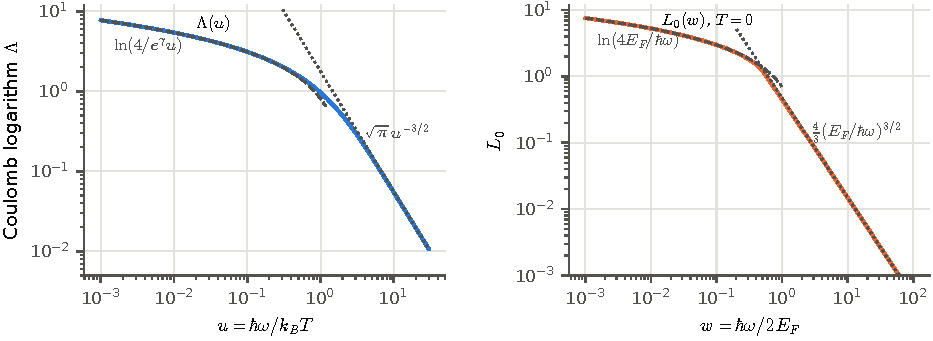
\includegraphics[width=\textwidth]{chapters/pd/fig_lambda.pdf}
\caption{Left, the Coulomb logarithm $\Lambda(u)$ of Maxwell electrons,
Eq.~\eqref{pd:eq:Lambda-mb}, with its asymptotes of
Eq.~\eqref{pd:eq:Lambda-limits}. Right, the function $L_0(w)$ of the degenerate
gas at $T=0$, Eq.~\eqref{pd:eq:nu-T0}, with its asymptotes of
Eq.~\eqref{pd:eq:L0-limits}, against $w=\hbar\omega/2E_F$.}
\label{pd:fig:lambda}
\end{figure}

\subsection{Arbitrary degeneracy}
\label{pd:sec:degenerate}
Insert Eq.~\eqref{pd:eq:imchi-fd} into Eq.~\eqref{pd:eq:nu-weak},
\begin{equation}
\boxed{\;\nueff=\frac{4Ze^4m\kB T}{3\pi\hbar^4\omega}\int_0^\infty\frac{\dd k}{k}\,
\ln\frac{1+e^{(\mu-E_-)/\kB T}}{1+e^{(\mu-E_+)/\kB T}},\qquad
E_\pm=\frac m2\Big(\frac\omega k\pm\frac{\hbar k}{2m}\Big)^2.\;}
\label{pd:eq:nu-fd}
\end{equation}
For $e^{\mu/\kB T}\ll1$ the logarithm is $e^{\mu/\kB T}(e^{-E_-/\kB T}-e^{-E_+/\kB T})$
and Eq.~\eqref{pd:eq:Lambda-mb} follows. The chemical potential is fixed by
$n_e=2\int\dd^3q\,(2\pi\hbar)^{-3}f$. Pauli blocking does not appear, by
Section~\ref{pd:sec:blocking}, but the occupation of the states does.

\subsection{The degenerate electron gas at zero temperature}
{\noindent}(1) At $T=0$, $\kB T\ln[(1+e^{(\mu-E_-)/\kB T})/(1+e^{(\mu-E_+)/\kB T})]
\to(E_F-E_-)_+-(E_F-E_+)_+$, where $(y)_+=\max(y,0)$ and $\mu=E_F=mv_F^2/2$.
With $x=k/k_F$, $k_F=mv_F/\hbar$ and $w=\hbar\omega/2E_F=\omega/k_Fv_F$,
$E_\pm/E_F=(w/x\pm x/2)^2$ and
\begin{equation}
\nueff=\frac{4Ze^4mE_F}{3\pi\hbar^4\omega}\,I_0(w),\qquad
I_0(w)=\int_0^\infty\frac{\dd x}{x}\Big\{\Big[1-\Big(\frac wx-\frac x2\Big)^2\Big]_+
-\Big[1-\Big(\frac wx+\frac x2\Big)^2\Big]_+\Big\}.
\end{equation}

{\noindent}(2) The first bracket is positive for $|w/x-x/2|<1$, that is for
$x_1<x<x_2$ with $x_{1,2}=\sqrt{1+2w}\mp1$. There the integrand is
$(1+w)/x-w^2/x^3-x/4$, with the antiderivative $(1+w)\ln x+w^2/2x^2-x^2/8$.
At the end points $w/x-x/2=\pm1$, and
$\tfrac12(w^2/x^2-x^2/4)=\tfrac12(w/x-x/2)(w/x+x/2)$ equals $(x_1+1)/2$ at $x_1$
and $-(x_2-1)/2$ at $x_2$. Hence
\begin{equation}
I_-(w)=(1+w)\ln\frac{\sqrt{1+2w}+1}{\sqrt{1+2w}-1}-\sqrt{1+2w}.
\end{equation}

{\noindent}(3) The second bracket is positive for $w/x+x/2<1$, which needs
$w<1/2$ and then $x_3<x<x_4$ with $x_{3,4}=1\mp\sqrt{1-2w}$. The same steps,
with the integrand $(1-w)/x-w^2/x^3-x/4$, give
\begin{equation}
I_+(w)=(1-w)\ln\frac{1+\sqrt{1-2w}}{1-\sqrt{1-2w}}-\sqrt{1-2w}\quad(w<\tfrac12),\qquad I_+=0\quad(w\geq\tfrac12).
\end{equation}

{\noindent}(4) With $4Ze^4mE_F/(3\pi\hbar^4\omega)=(4Ze^4m/3\pi\hbar^3)/(2w)$,
\begin{equation}
\boxed{\;\nueff=\frac{4Ze^4m}{3\pi\hbar^3}\,L_0(w),\qquad L_0(w)=\frac{I_-(w)-I_+(w)}{2w},\qquad
w=\frac{\hbar\omega}{2E_F}.\;}
\label{pd:eq:nu-T0}
\end{equation}

{\noindent}(5) For $w\ll1$, $I_-(w)-I_+(w)=2w\ln(2/w)+O(w^2)$, and for
$w\gg1$, $I_-=\tfrac43(2w)^{-1/2}+O(w^{-3/2})$, so
\begin{equation}
\boxed{\;L_0(w)\simeq\ln\frac{4E_F}{\hbar\omega}\quad(\hbar\omega\ll E_F),\qquad
L_0(w)\simeq\frac43\Big(\frac{E_F}{\hbar\omega}\Big)^{3/2}\quad(\hbar\omega\gg E_F).\;}
\label{pd:eq:L0-limits}
\end{equation}
{\noindent}(6) The low-frequency form is the resistivity formula of Ziman.
For an electron at the Fermi surface the Born cross section
$(m/2\pi\hbar^2)^2|\tilde v(q)|^2$ with $q=2k_F\sin(\theta/2)$,
$1-\cos\theta=q^2/2k_F^2$ and $\dd\Omega=2\pi q\,\dd q/k_F^2$ gives the momentum
relaxation rate
\begin{equation}
\frac1\tau=n_iv_F\int(1-\cos\theta)\frac{\dd\sigma}{\dd\Omega}\dd\Omega
=\frac{n_im}{4\pi\hbar^3k_F^3}\int_{k_{\min}}^{2k_F}q^3|\tilde v(q)|^2\,\dd q
=\frac{4Ze^4m}{3\pi\hbar^3}\ln\frac{2k_F}{k_{\min}},
\end{equation}
where the last step uses the Coulomb form and $k_F^3=3\pi^2n_e=3\pi^2Zn_i$.
With the minimum momentum transfer $k_{\min}=\omega/v_F$ that energy
conservation imposes on an electron at the Fermi surface,
$\ln(2k_F/k_{\min})=\ln(4E_F/\hbar\omega)$, and the two agree.

\subsection{The universal high-frequency tail}
{\noindent}(1) When $\hbar\omega$ exceeds every electron energy that is
occupied, Eq.~\eqref{pd:eq:imchi-general} has $E_+=E_-+\hbar\omega$ far above the
occupied energies, and $E_-$ is small only near $k_\omega=(2m\omega/\hbar)^{1/2}$,
where $\omega/k=\hbar k/2m$. There $c_-=\omega/k-\hbar k/2m\simeq-(\hbar/m)(k-k_\omega)$.

{\noindent}(2) Hence
\begin{equation}
\int_0^\infty\frac{\dd k}{k}\int_{E_-}^{E_+}f\,\dd E\simeq\frac{m}{\hbar k_\omega}
\int_{-\infty}^\infty\dd c\int_{mc^2/2}^\infty f(E)\,\dd E
=\frac{m}{\hbar k_\omega}\,2\int_0^\infty f(E)\Big(\frac{2E}{m}\Big)^{1/2}\dd E
=\frac{m}{\hbar k_\omega}\,\frac{n_e(2\pi\hbar)^3}{4\pi m^2},
\end{equation}
where the last step uses $n_e=8\pi m(2\pi\hbar)^{-3}\int(2mE)^{1/2}f\,\dd E$.

{\noindent}(3) With Eq.~\eqref{pd:eq:imchi-general}, $\int_0^\infty\Imag\chi_0\,\dd k=-\pi mn_e/\hbar^2k_\omega$
for every distribution, and Eq.~\eqref{pd:eq:nu-weak} gives
\begin{equation}
\boxed{\;\nueff\;\longrightarrow\;\frac{4\sqrt2\,\pi}{3}\,\frac{Zn_ee^4}{m^{1/2}(\hbar\omega)^{3/2}}.\;}
\label{pd:eq:tail}
\end{equation}
Both the Maxwell form, $\nuT\sqrt\pi u^{-3/2}$, and the degenerate form,
$(4Ze^4m/3\pi\hbar^3)\tfrac43(E_F/\hbar\omega)^{3/2}$ with
$E_F^{3/2}=3\pi^2\hbar^3n_e/(2m)^{3/2}$, reduce to it. When the photon energy
exceeds the kinetic energies the electrons absorb as if they were at rest.

\medskip
\noindent\textbf{Remarks:}\\
(1) For hydrogen at $\kB T=1$~keV and $\lambda_L=0.351~\mu$m,
$u=0.0035$ and $\Lambda=6.45$, while the logarithm of the cutoffs stated
with Eq.~(10.136)~\cite{pd:Atzeni2004} at $n_e=n_c/4$ is $7.58$, and the printed
formula gives $6.69$. The difference between the printed formula and its
stated cutoffs is taken up in Appendix~\ref{pd:app:atzeni-log}.\\
(2) Screening changes the lower limit of the $k$ integral, where $\Imag\chi_0$
is already exponentially small below $k\sim\omega/v_t$. Its effect is computed
in Section~\ref{pd:sec:rpa} and is a few tenths in $\Lambda$ near the critical
density.


\section{Spontaneous bremsstrahlung, the Gaunt factor and Kirchhoff's law}
\label{pd:sec:gaunt}
\subsection{From stimulated to spontaneous emission}
{\noindent}(1) Quantize one mode of the radiation field in the box, with wave
vector $\kv_L$, polarization $\ehat_\lambda$ and frequency $\omega=ck_L$,
\begin{equation}
\hat\Ev=i\Big(\frac{2\pi\hbar\omega}{\Vol}\Big)^{1/2}\ehat_\lambda
\big(\hat a\,e^{i(\kv_L\cdot\rv-\omega t)}-\hat a^\dagger e^{-i(\kv_L\cdot\rv-\omega t)}\big).
\end{equation}
In a state with $N$ photons the absorption matrix element carries
$\langle N-1|\hat a|N\rangle=\sqrt N$ and the emission one
$\langle N+1|\hat a^\dagger|N\rangle=\sqrt{N+1}$.

{\noindent}(2) The classical field $E_0\ehat\cos\omega t$ has the amplitude
$E_0/2$ in front of $e^{-i\omega t}$. For $N\gg1$ it corresponds to
$E_0/2=(2\pi\hbar\omega N/\Vol)^{1/2}$, that is $E_0^2/8\pi=N\hbar\omega/\Vol$, the
energy density of $N$ photons. The weak-field rates of
Section~\ref{pd:sec:onephoton} are therefore $N$ times the rates for one photon,
and the spontaneous emission into the mode is the stimulated rate with
$N\to1$,
\begin{equation}
\boxed{\;W^{\rm sp}_{\pv\to\pv'}(\kv_L,\lambda)=W_{\pv\to\pv'}^{(\ell=-1)}\Big|_{E_0^2=8\pi\hbar\omega/\Vol,\;\ehat=\ehat_\lambda}.\;}
\label{pd:eq:spont-stim}
\end{equation}
This is the content of Einstein's relation, Eqs.~(10.84) and (10.85)~\cite{pd:Atzeni2004}.

\subsection{The Born bremsstrahlung cross section}
{\noindent}(1) With $a_0^2=e^2E_0^2/m^2\omega^4=8\pi\hbar e^2/(\Vol m^2\omega^3)$,
the cross section of Eq.~\eqref{pd:eq:bf} for $\ell=-1$ and one mode is
\begin{equation}
\frac{\dd\sigma}{\dd\Omega'}=\frac{m^2}{4\pi^2\hbar^4}\frac{p'}{p}|\tilde v(\kv)|^2\,
\frac{(\kv\cdot\ehat_\lambda)^2}{4}\,\frac{8\pi\hbar e^2}{\Vol m^2\omega^3}
=\frac{e^2}{2\pi\hbar^3\Vol\omega^3}\,\frac{p'}{p}\,|\tilde v(\kv)|^2(\kv\cdot\ehat_\lambda)^2,
\end{equation}
with $p'=(p^2-2m\hbar\omega)^{1/2}$.

{\noindent}(2) Sum over the modes in vacuum,
$\sum_{\kv_L,\lambda}\to\Vol\sum_\lambda\int\omega^2\dd\omega\,\dd\Omega_L/(2\pi c)^3$.
The two polarizations perpendicular to $\hat\kv_L$ give
$\sum_\lambda(\kv\cdot\ehat_\lambda)^2=k^2-(\kv\cdot\hat\kv_L)^2$, whose integral
over the directions of the photon is $4\pi k^2-\tfrac{4\pi}{3}k^2=\tfrac{8\pi}{3}k^2$.
The emission cross section per unit frequency is
\begin{equation}
\frac{\dd\sigma}{\dd\omega\,\dd\Omega'}=\frac{e^2}{2\pi\hbar^3\omega^3}\,\frac{\omega^2}{8\pi^3c^3}\,
\frac{8\pi}{3}\,\frac{p'}{p}\,k^2|\tilde v(\kv)|^2
=\frac{e^2}{6\pi^3\hbar^3c^3\omega}\,\frac{p'}{p}\,k^2|\tilde v(\kv)|^2.
\label{pd:eq:spont-diff}
\end{equation}

{\noindent}(3) For a Coulomb ion $k^2|\tilde v|^2=16\pi^2Z^2e^4/k^2$, and
$\int\dd\Omega'/k^2=2\pi\hbar^2\int_{-1}^1\dd c/(p^2+p'^2-2pp'c)=(2\pi\hbar^2/pp')L$
with $L=\ln[(p+p')/(p-p')]$, so
\begin{equation}
\boxed{\;\frac{\dd\sigma}{\dd\omega}=\frac{16}{3}\,\frac{Z^2e^6}{m^2c^3\hbar v^2\omega}\,
\ln\frac{p+p'}{p-p'}.\;}
\label{pd:eq:born-brems}
\end{equation}
This is the nonrelativistic Born cross section of bremsstrahlung,
$\dd\sigma=\tfrac{16}{3}Z^2\alpha r_e^2(c^2/v^2)L\,\dd\omega/\omega$ with
$\alpha=e^2/\hbar c$ and $r_e=e^2/mc^2$.

{\noindent}(4) Kramers' cross section of Eq.~\eqref{pd:eq:kramers}, per unit
angular frequency, is $(\dd\sigma/\dd\nu)/2\pi$ with $h\nu=\hbar\omega$, that is
$(16\pi/3\sqrt3)Z^2e^6/(m^2c^3v^2\hbar\omega)$. The ratio is the Born Gaunt factor,
\begin{equation}
\boxed{\;g_B(E,\hbar\omega)=\frac{\sqrt3}{\pi}\ln\frac{p+p'}{p-p'},\qquad
p=(2mE)^{1/2},\quad p'=[2m(E-\hbar\omega)]^{1/2}.\;}
\label{pd:eq:gaunt-born}
\end{equation}
For soft photons $g_B\to(\sqrt3/\pi)\ln(4E/\hbar\omega)$, and at the threshold
$p'\to0$ it vanishes as $(\sqrt3/\pi)2p'/p$.

\subsection{The thermal average}
{\noindent}(1) The emission of a Maxwellian plasma is proportional to
$\int\dd^3v\,f\,v\,\dd\sigma/\dd\omega\propto\int v\,\dd v\,e^{-E/\kB T}g_B
=m^{-1}\int\dd E\,e^{-E/\kB T}g_B$ over $E>\hbar\omega$, while Kramers' form
has $g=1$. The thermally averaged Gaunt factor is therefore
\begin{equation}
\langle g\rangle=\frac{\int_{\hbar\omega}^\infty e^{-E/\kB T}g_B\,\dd E}{\int_{\hbar\omega}^\infty e^{-E/\kB T}\dd E}
=\frac{\sqrt3}{\pi}\,e^u\int_u^\infty e^{-\epsilon}
\ln\frac{\sqrt\epsilon+\sqrt{\epsilon-u}}{\sqrt\epsilon-\sqrt{\epsilon-u}}\,\dd\epsilon,
\end{equation}
with $\epsilon=E/\kB T$.

{\noindent}(2) Substitute $\epsilon=u\cosh^2t$. Then
$\sqrt\epsilon\pm\sqrt{\epsilon-u}=\sqrt u\,e^{\pm t}$, the logarithm is $2t$, and
$\dd\epsilon=u\sinh2t\,\dd t$. With $\cosh^2t=\tfrac12(1+\cosh2t)$ and $\tau=2t$,
\begin{equation}
\int_u^\infty e^{-\epsilon}\ln(\cdots)\,\dd\epsilon
=\frac u2\,e^{-u/2}\int_0^\infty\tau\sinh\tau\,e^{-(u/2)\cosh\tau}\dd\tau.
\end{equation}

{\noindent}(3) Integrate by parts with
$\sinh\tau\,e^{-(u/2)\cosh\tau}=\dd[-(2/u)e^{-(u/2)\cosh\tau}]/\dd\tau$. The
boundary terms vanish, and $\int_0^\infty e^{-z\cosh\tau}\dd\tau=K_0(z)$,
Eq.~(10.32.9)~\cite{pd:DLMF}, leaves $(2/u)K_0(u/2)$. Hence
\begin{equation}
\boxed{\;\langle g\rangle(u)=\frac{\sqrt3}{\pi}\,e^{u/2}K_0\Big(\frac u2\Big).\;}
\label{pd:eq:gaunt-avg}
\end{equation}

{\noindent}(4) The power radiated at all frequencies weights the spectrum
with $e^{-u}$, the factor of Kramers' form, so its Gaunt factor is
\begin{equation}
\boxed{\;\bar g=\int_0^\infty\langle g\rangle(u)\,e^{-u}\,\dd u=\frac{\sqrt3}{\pi}\,2\int_0^\infty e^{-x}K_0(x)\,\dd x
=\frac{2\sqrt3}{\pi}=1.103,\;}
\label{pd:eq:gaunt-power}
\end{equation}
using $K_0(x)=\int_0^\infty e^{-x\cosh t}\dd t$, so that
$\int_0^\infty e^{-x}K_0(x)\dd x=\int_0^\infty\dd t/(1+\cosh t)=[\tanh(t/2)]_0^\infty=1$.
This is the factor $g\approx2\sqrt3/\pi$ that
Atzeni and Meyer-ter-Vehn apply to Eq.~(10.93)~\cite{pd:Atzeni2004}. It is the
Born value exactly.

\subsection{Kirchhoff's law and the Coulomb logarithm as a Gaunt factor}
{\noindent}(1) Compare Eq.~\eqref{pd:eq:gaunt-avg} with Eq.~\eqref{pd:eq:Lambda-mb},
\begin{equation}
\boxed{\;\Lambda(u)=\frac{\pi}{\sqrt3}\,\langle g\rangle(u)\,\frac{1-e^{-u}}{u}.\;}
\label{pd:eq:Lambda-gaunt}
\end{equation}
The quantum Coulomb logarithm of inverse bremsstrahlung is $\pi/\sqrt3$ times
the thermally averaged Gaunt factor, times the stimulated-emission factor
divided by $u$.

{\noindent}(2) The emission coefficient per unit volume, frequency and solid
angle follows from Eq.~\eqref{pd:eq:born-brems} and the steps of the thermal
average,
\begin{equation}
\begin{aligned}
j_\omega&=\frac{n_en_i\hbar\omega}{4\pi}\Big\langle v\,\frac{\dd\sigma}{\dd\omega}\Big\rangle,\qquad
\Big\langle\frac Lv\Big\rangle=\Big(\frac2\pi\Big)^{1/2}\frac{\pi}{\sqrt3}\,\frac{\langle g\rangle e^{-u}}{v_t},\\
j_\omega&=\frac{4}{3\pi}\Big(\frac2\pi\Big)^{1/2}\frac{n_en_iZ^2e^6}{m^2c^3v_t}\,\frac{\pi}{\sqrt3}\langle g\rangle e^{-u}.
\end{aligned}
\end{equation}
The absorption coefficient of Eq.~\eqref{pd:eq:drude-K} with $n_r=1$ and
$\nueff=\nuT\Lambda$, multiplied by the Planck function per unit angular
frequency and solid angle, $B_\omega=(\hbar\omega^3/4\pi^3c^2)/(e^u-1)$, is, by
Eq.~\eqref{pd:eq:Lambda-gaunt},
\begin{equation}
K\,B_\omega=\frac{\nuT\omega_p^2}{c\omega^2}\,\frac{\pi}{\sqrt3}\langle g\rangle\frac{e^{-u}}{u}\,\frac{\hbar\omega^3}{4\pi^3c^2}
=\frac{4\sqrt{2\pi}}{3\pi^2}\,\frac{n_en_iZ^2e^6}{m^{3/2}(\kB T)^{1/2}c^3}\,\frac{\pi}{\sqrt3}\langle g\rangle e^{-u}.
\end{equation}
Since $m^2v_t=m^{3/2}(\kB T)^{1/2}$ and $\tfrac{4}{3\pi}(2/\pi)^{1/2}=\tfrac{4\sqrt{2\pi}}{3\pi^2}$,
\begin{equation}
\boxed{\;j_\omega=K\,B_\omega.\;}
\label{pd:eq:kirchhoff}
\end{equation}
Kirchhoff's law holds exactly between the absorption of the master equation
and the spontaneous emission of Eq.~\eqref{pd:eq:born-brems}, because both come
from the same matrix element and the Maxwellian satisfies detailed balance.

\medskip
\noindent\textbf{In Summary:} The free--free emission and the inverse
bremsstrahlung absorption of the quantum theory are Kramers' expressions
multiplied by the Born Gaunt factor. Its thermal average is
$(\sqrt3/\pi)e^{u/2}K_0(u/2)$, its power average is $2\sqrt3/\pi$, and the
Coulomb logarithm of the absorption is the Gaunt factor in disguise,
Eq.~\eqref{pd:eq:Lambda-gaunt}.

\section{The interacting electron gas and dynamic screening}
\label{pd:sec:manybody}
\subsection{The oscillating frame for many electrons}
{\noindent}(1) The Hamiltonian of $N$ electrons in the laser field and the
field of the ions is
\begin{equation}
H=\sum_{a=1}^N\frac{1}{2m}\Big[\hat\pv_a+\frac ec\Av(t)\Big]^2
+\sum_{a<b}\frac{e^2}{|\hat\rv_a-\hat\rv_b|}+\sum_aV(\hat\rv_a),
\end{equation}
apart from the constant energy of the fixed ions.

{\noindent}(2) Let $\hat T=\exp[-(i/\hbar)\boldsymbol\alpha(t)\cdot\hat{\mathbf P}]$
with $\hat{\mathbf P}=\sum_a\hat\pv_a$. It translates all electrons together, so
the electron--electron interaction, which depends on differences, is
unchanged, $\hat T^\dagger V_{ee}\hat T=V_{ee}$. The steps of
Section~\ref{pd:sec:KH1}, with $\dot S=Ne^2A^2/2mc^2$, give
\begin{equation}
\boxed{\;H'=\sum_a\frac{\hat p_a^2}{2m}+\sum_{a<b}\frac{e^2}{|\hat\rv_a-\hat\rv_b|}
+\sum_aV\big(\hat\rv_a+\boldsymbol\alpha(t)\big).\;}
\label{pd:eq:H-KH}
\end{equation}
In the oscillating frame the electron gas carries no field, and the ions are
external charges that move along $\Rv_j-\boldsymbol\alpha(t)$. A uniform field
couples only to the center of mass of the electrons \cite{pd:Kohn1961}, which is
the content of this transformation.

\subsection{The absorbed power in the two frames}
{\noindent}(1) The power that the laser delivers to the electrons in the
laboratory is $P_{\rm lab}(t)=-e\Ev(t)\cdot\sum_a\langle\vv_a\rangle$, with the
velocity $\vv_a=(\hat\pv_a+e\Av/c)/m$. Since $\hat T$ commutes with
$\hat\pv_a$, $\sum_a\langle\vv_a\rangle=\langle\hat{\mathbf P}\rangle'/m+N\dot{\boldsymbol\alpha}$,
where the prime marks an average in the oscillating frame. The term
$-eN\Ev\cdot\dot{\boldsymbol\alpha}\propto\cos\omega t\sin\omega t$ averages to
zero over a period.

{\noindent}(2) In the oscillating frame,
$\dd\langle H'\rangle/\dd t=\langle\partial_tH'\rangle=-\dot{\boldsymbol\alpha}\cdot\langle\mathbf F\rangle'$,
with the force $\mathbf F=-\sum_a\nabla V(\hat\rv_a+\boldsymbol\alpha)$ of the ions
on the electrons. The total momentum obeys
$\dd\langle\hat{\mathbf P}\rangle'/\dd t=\langle\mathbf F\rangle'$, because the
kinetic term commutes with $\hat{\mathbf P}$ and the internal forces cancel.
With $\ddot{\boldsymbol\alpha}=-e\Ev/m$,
\begin{equation}
\frac{\dd\langle H'\rangle}{\dd t}=-\dot{\boldsymbol\alpha}\cdot\frac{\dd\langle\hat{\mathbf P}\rangle'}{\dd t}
=-\frac{\dd}{\dd t}\big(\dot{\boldsymbol\alpha}\cdot\langle\hat{\mathbf P}\rangle'\big)
-\frac em\Ev\cdot\langle\hat{\mathbf P}\rangle'.
\end{equation}

{\noindent}(3) In the steady state $\langle\hat{\mathbf P}\rangle'$ is
periodic, and the total derivative averages to zero. Hence
\begin{equation}
\boxed{\;\langle P_{\rm lab}\rangle_t=\Big\langle\frac{\dd\langle H'\rangle}{\dd t}\Big\rangle_t.\;}
\label{pd:eq:frames}
\end{equation}
The absorbed power is the rate at which the energy of the electron gas grows
in the oscillating frame.

\subsection{Linear response to the oscillating ions}
{\noindent}(1) With the density operator $\hat n_{\kv}=\sum_ae^{-i\kv\cdot\hat\rv_a}$
and Eq.~\eqref{pd:eq:Vk}, the ion term of Eq.~\eqref{pd:eq:H-KH} is
\begin{equation}
\sum_aV(\hat\rv_a+\boldsymbol\alpha)=\frac1\Vol\sum_{\kv}U_{\kv}(t)\,\hat n_{-\kv},\qquad
U_{\kv}(t)=\tilde V(\kv)\,e^{i\kv\cdot\boldsymbol\alpha(t)}
=\tilde V(\kv)\sum_\ell i^\ell J_\ell(\kv\cdot\av)\,e^{i\ell\omega t},
\label{pd:eq:Uk}
\end{equation}
by Eq.~\eqref{pd:eq:jacobi-anger}. In this frame the ion potential is a sum of
harmonics $\ell\omega$ with the weights $J_\ell$.

{\noindent}(2) Let the electron gas start in equilibrium. To first order in
$U$, Kubo's formula gives
$\delta\langle\hat n_{\kv}\rangle'(t)=\int\chi(\kv,t-t')U_{\kv}(t')\dd t'$ with
the retarded density response
\begin{equation}
\chi(\kv,t)=-\frac i\hbar\,\theta(t)\,\frac1\Vol\big\langle[\hat n_{\kv}(t),\hat n_{-\kv}(0)]\big\rangle,\qquad
\chi(\kv,\Omega)=\int e^{i\Omega t}\chi(\kv,t)\,\dd t,
\end{equation}
which for free electrons is the Lindhard function of Eq.~\eqref{pd:eq:chi0}
\cite{pd:GiulianiVignale2005}. A harmonic $e^{i\ell\omega t}=e^{-i(-\ell\omega)t}$
is answered with the factor $\chi(\kv,-\ell\omega)$.

{\noindent}(3) The power in the oscillating frame is
$\dd\langle H'\rangle/\dd t=\Vol^{-1}\sum_{\kv}\partial_tU_{\kv}\,\langle\hat n_{-\kv}\rangle'$.
The term $\kv=0$ is constant. With
$U_{-\kv}=\tilde V(-\kv)\sum_\ell(-i)^\ell J_\ell(\kv\cdot\av)e^{i\ell\omega t}$, the
response $\delta\langle\hat n_{-\kv}\rangle'=\sum_\ell\chi(-\kv,-\ell\omega)U_{-\kv,\ell}e^{i\ell\omega t}$,
and $\partial_tU_{\kv}=\sum_{\ell'}i\ell'\omega U_{\kv,\ell'}e^{i\ell'\omega t}$, the
period average keeps $\ell'=-\ell$. The product of the coefficients is
$\tilde V(\kv)\tilde V(-\kv)\,i^{-\ell}J_{-\ell}(-i)^\ell J_\ell=|\tilde V(\kv)|^2J_\ell^2$,
and with $\chi(-\kv,-\Omega)=\chi(\kv,\Omega)^*$,
\begin{equation}
\Big\langle\frac{\dd\langle H'\rangle}{\dd t}\Big\rangle_t
=\frac1\Vol\sum_{\kv}\sum_\ell(-i\ell\omega)|\tilde V(\kv)|^2J_\ell^2\,\chi(\kv,\ell\omega)^*
=-\frac1\Vol\sum_{\kv}\sum_\ell\ell\omega\,|\tilde V(\kv)|^2J_\ell^2\,\Imag\chi(\kv,\ell\omega),
\end{equation}
where the terms with $\Real\chi$, which is even in the frequency for the
isotropic gas, cancel between $\ell$ and $-\ell$.

{\noindent}(4) After the average over the ion positions and per unit
volume, by Eq.~\eqref{pd:eq:frames},
\begin{equation}
\boxed{\;P=-n_i\sum_{\ell=-\infty}^\infty\ell\omega\int\frac{\dd^3k}{(2\pi)^3}\,|\tilde v(\kv)|^2S(\kv)\,
J_\ell^2(\kv\cdot\av)\,\Imag\chi(\kv,\ell\omega).\;}
\label{pd:eq:P-KH}
\end{equation}
This is Eq.~\eqref{pd:eq:P-chi0} with $\chi_0$ replaced by the density response
of the interacting gas. For free electrons the two derivations agree term by
term, because the Volkov states of the laboratory are the plane waves of the
oscillating frame. The result is exact to second order in the ion potential
and exact in the field.

\subsection{The dielectric form}
{\noindent}(1) The longitudinal dielectric function is defined by
$1/\varepsilon(\kv,\Omega)=1+v_c(k)\chi(\kv,\Omega)$ with $v_c=4\pi e^2/k^2$.
In the random-phase approximation $\varepsilon=1-v_c\chi_0$ and $\chi=\chi_0/\varepsilon$.
For a Coulomb ion,
$|\tilde v|^2\Imag\chi=(4\pi Ze^2/k^2)^2(k^2/4\pi e^2)\Imag\varepsilon^{-1}=(4\pi Z^2e^2/k^2)\Imag\varepsilon^{-1}$,
and
\begin{equation}
\boxed{\;P=-n_iZ^2e^2\sum_{\ell=-\infty}^\infty\ell\omega\int\frac{\dd^3k}{(2\pi)^3}\,\frac{4\pi}{k^2}\,S(\kv)\,
J_\ell^2(\kv\cdot\av)\,\Imag\frac{1}{\varepsilon(\kv,\ell\omega)}.\;}
\label{pd:eq:P-silin}
\end{equation}
With the classical dielectric function this is Silin's result \cite{pd:Silin1965}.
With the Lindhard dielectric function it is the quantum form obtained by Kull
and Plagne \cite{pd:KullPlagne2001} and by Bornath and co-workers
\cite{pd:Bornath2001} from the quantum Vlasov and the quantum kinetic equation.

{\noindent}(2) For weak fields Eq.~\eqref{pd:eq:nu-weak} with
$k^4|\tilde v|^2\Imag\chi=4\pi Z^2e^2k^2\Imag\varepsilon^{-1}$ gives
\begin{equation}
\boxed{\;\nueff(\omega)=-\frac{2Ze^2}{3\pi m\omega}\int_0^\infty k^2S(k)\,\Imag\frac{1}{\varepsilon(k,\omega)}\,\dd k,\;}
\label{pd:eq:dawson-oberman}
\end{equation}
the high-frequency collision frequency of Dawson and Oberman
\cite{pd:DawsonOberman1962}.

\subsection{Dynamic screening for Maxwell electrons}
\label{pd:sec:rpa}
{\noindent}(1) For nondegenerate electrons the Lindhard function follows from
Eq.~\eqref{pd:eq:chi0} with the shift $\mathbf q\to\mathbf q-\hbar\kv$ in its
second term and the integral over $\mathbf q_\perp$, which leaves the
one-dimensional Maxwellian $g_1(v)=(2\pi v_t^2)^{-1/2}e^{-v^2/2v_t^2}$,
\begin{equation}
\chi_0=\frac{n_e}{\hbar k}\int g_1(v)\Big[\frac{1}{c_--v+i0^+}-\frac{1}{c_+-v+i0^+}\Big]\dd v
=\frac{n_e}{\sqrt2\,\hbar kv_t}\big[Z(\zeta_+)-Z(\zeta_-)\big],\qquad
\zeta_\pm=\frac{c_\pm}{\sqrt2v_t},
\label{pd:eq:chi0-Z}
\end{equation}
with $c_\pm=\Omega/k\pm\hbar k/2m$ and the plasma dispersion function
$Z(\zeta)=\pi^{-1/2}\int e^{-t^2}(t-\zeta)^{-1}\dd t$ for $\Imag\zeta>0$
\cite{pd:FriedConte1961}. Its imaginary part on the real axis is
$\sqrt\pi e^{-\zeta^2}$, which gives back Eq.~\eqref{pd:eq:imchi-mb}.

{\noindent}(2) In the classical limit $Z(\zeta_+)-Z(\zeta_-)\to(\hbar k/\sqrt2mv_t)Z'(\zeta)$
with $Z'=-2(1+\zeta Z)$, so $\chi_0\to-(n_e/\kB T)[1+\zeta Z(\zeta)]$ and
$\varepsilon=1+(k_D^2/k^2)[1+\zeta Z(\zeta)]$ with $k_D^2=4\pi e^2n_e/\kB T$. This is
Eq.~(11.19)~\cite{pd:Atzeni2004}, whose function $W$ is $W(x)=1+(x/\sqrt2)Z(x/\sqrt2)$.

{\noindent}(3) With $x=kv_t/\omega$, $r=\omega_p/\omega$, $\hbar kv_t/\kB T=ux$ and
$k_D^2/k^2=r^2/x^2$,
\begin{equation}
\varepsilon(x)=1-\frac{r^2}{\sqrt2\,ux^3}\big[Z(\zeta_+)-Z(\zeta_-)\big],\qquad
\zeta_\pm=\frac{1}{\sqrt2}\Big(\frac1x\pm\frac{ux}{2}\Big).
\end{equation}
Equation~\eqref{pd:eq:dawson-oberman} with $S=1$, divided by $\nuT$, becomes
\begin{equation}
\boxed{\;\nueff=\nuT\Lambda_{\rm RPA}(r,u),\qquad
\Lambda_{\rm RPA}(r,u)=-\frac{1}{r^2}\Big(\frac2\pi\Big)^{1/2}\int_0^\infty x^2\,\Imag\frac{1}{\varepsilon(x)}\,\dd x.\;}
\label{pd:eq:Lambda-rpa}
\end{equation}
Without screening $\Imag\varepsilon^{-1}\to-\Imag\varepsilon$, the integral
becomes $u^{-1}\int x^{-1}[e^{-\zeta_-^2}-e^{-\zeta_+^2}]\dd x$, and
Eq.~\eqref{pd:eq:Lambda-mb} returns.

{\noindent}(4) Table~\ref{pd:tab:rpa} and Fig.~\ref{pd:fig:rpa} give the screening correction. It is
negative and nearly independent of $u$. It is $-0.10$ at $n_e=n_c/4$ and $-0.47$ at
$n_e=0.94\,n_c$, and it approaches $-0.56$ as $\omega\to\omega_p$ for $u\ll1$, slowly,
because the resonance described next carries a weight proportional to
$(1-r^2)^{1/2}$. For $\omega>\omega_p$ the function $\Real\varepsilon$ vanishes
at the Langmuir wave number, approximately $x_{\rm pl}^2=(r^{-2}-1)/3$, where
the ion oscillation excites plasma waves. That resonance is part of the
integral. Its weight, estimated with the Bohm--Gross form
$\Real\varepsilon\simeq1-r^2(1+3x^2)$, is $\sqrt{2\pi}\,x_{\rm pl}/6r^4$, of order
$0.1$ for $r\geq0.9$. For smaller $r$ the plasma waves at $x_{\rm pl}$ are
strongly Landau damped and there is no separate resonance.

\begin{table}[ht]
\centering
\caption{The screening correction $\Lambda_{\rm RPA}-\Lambda$ of the Coulomb
logarithm, Eqs.~\eqref{pd:eq:Lambda-rpa} and \eqref{pd:eq:Lambda-mb}, against
$r=\omega_p/\omega=(n_e/n_c)^{1/2}$.}
\label{pd:tab:rpa}
\begin{tabular}{cccccccc}
\toprule
$u$ & $r=0.95$ & $0.9$ & $0.8$ & $0.7$ & $0.5$ & $0.3$ & $0.1$\\
\midrule
0.003 & $-0.440$ & $-0.375$ & $-0.278$ & $-0.204$ & $-0.099$ & $-0.034$ & $-0.004$\\
0.03  & $-0.439$ & $-0.374$ & $-0.277$ & $-0.203$ & $-0.098$ & $-0.034$ & $-0.004$\\
0.3   & $-0.393$ & $-0.333$ & $-0.244$ & $-0.178$ & $-0.085$ & $-0.029$ & $-0.003$\\
\bottomrule
\end{tabular}
\end{table}

\begin{figure}[ht]
\centering
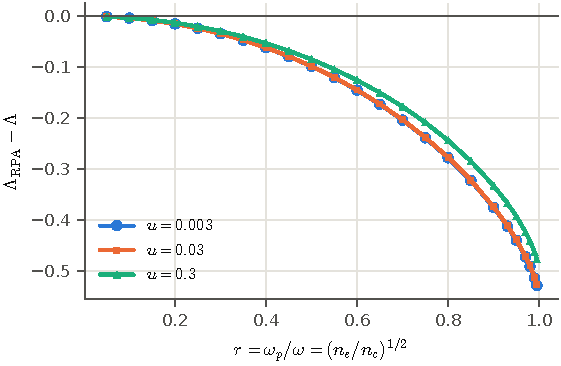
\includegraphics[width=0.62\textwidth]{chapters/pd/fig_rpa.pdf}
\caption{The screening correction $\Lambda_{\rm RPA}-\Lambda$ of
Table~\ref{pd:tab:rpa} against $r=\omega_p/\omega$ for three photon energies.}
\label{pd:fig:rpa}
\end{figure}

\medskip
\noindent\textbf{Remarks:}\\
(1) Without ions $H'$ does not depend on time and nothing is absorbed.
Collisions between electrons alone do not absorb light in the dipole
approximation. They enter only through $\chi$, by screening, and through the
shape of $f$.\\
(2) Equation~\eqref{pd:eq:P-KH} holds for any response function. Local-field
corrections and strong coupling enter through $\chi$, and correlated ions
through $S(k)$.\\
(3) The same result follows from the Kadanoff--Baym equations with the
dynamically screened Born self-energy \cite{pd:Kremp1999,pd:Bornath2001}, which is the
many-body counterpart of the nonequilibrium Green-function route of
Section~3 of the quantum Boltzmann equation paper \cite{pd:Watson2026}.


\section{Strong fields}
\label{pd:sec:strong}
\subsection{The exact heating rate for Maxwell electrons}
{\noindent}(1) Take Eq.~\eqref{pd:eq:P-chi0} with bare Coulomb ions, $S=1$ and an
isotropic distribution. At fixed $k$ the direction of $\kv$ enters only through
$\mu=\hat\kv\cdot\ehat$, and $\int\dd\Omega_kJ_\ell^2(ka_0\mu)=2\pi B_\ell(ka_0)$
with
\begin{equation}
B_\ell(z)=\int_{-1}^1J_\ell^2(z\mu)\,\dd\mu=\frac2z\int_0^zJ_\ell^2(t)\,\dd t.
\end{equation}
With $|\tilde v|^2=16\pi^2Z^2e^4/k^4$,
\begin{equation}
P=-4n_iZ^2e^4\sum_\ell\ell\omega\int_0^\infty\frac{\dd k}{k^2}\,\Imag\chi_0(k,\ell\omega)\,B_\ell(ka_0).
\end{equation}

{\noindent}(2) With $x=kv_t/\omega$ and $\beta=v_0/v_t$, $ka_0=x\beta$, and
Eq.~\eqref{pd:eq:imchi-mb} at $\Omega=\ell\omega$ has
$E_\pm/\kB T=\tfrac12(\ell/x\pm ux/2)^2$ and $\hbar kv_t=ux\,\kB T$. Dividing by
$n_emv_0^2/2$ and by $\nuT$,
\begin{equation}
\boxed{\;\begin{aligned}
\nueff&=\nuT\,\frac{3\,\mathcal S(\beta,u)}{u\beta^2},\qquad
\mathcal S(\beta,u)=\sum_{\ell=-\infty}^\infty\ell\int_0^\infty\frac{\dd x}{x^3}\,D_\ell(x)\,B_\ell(x\beta),\\
D_\ell(x)&=e^{-\frac12(\frac\ell x-\frac{ux}2)^2}-e^{-\frac12(\frac\ell x+\frac{ux}2)^2}.
\end{aligned}\;}
\label{pd:eq:S-exact}
\end{equation}
The terms $\pm\ell$ are equal. For $\beta\to0$, $B_{\pm1}\to(x\beta)^2/6$, and
Eq.~\eqref{pd:eq:K0-integral} gives the weak-field limit on the left below,
which is Eq.~\eqref{pd:eq:Lambda-mb}. The nonlinearity is measured by the ratio
on the right,
\begin{equation}
\mathcal S\;\xrightarrow{\;\beta\to0\;}\;\frac{\beta^2}{3}\,2\sinh\frac u2\,K_0\Big(\frac u2\Big),\qquad
R(\beta,u)=\frac{\nueff(v_0)}{\nueff(0)}=\frac{3\,\mathcal S(\beta,u)}{u\beta^2\Lambda(u)}.
\end{equation}

{\noindent}(3) The functions $B_\ell$ follow from a recursion. The recurrences
of the Bessel functions, Eq.~(10.6.2)~\cite{pd:DLMF}, give
$\dd[z(J_\ell^2+J_{\ell+1}^2)]/\dd z=(2\ell+1)(J_\ell^2-J_{\ell+1}^2)$, so
\begin{equation}
\int_0^zJ_\ell^2\,\dd t=\int_0^zJ_{\ell+1}^2\,\dd t+\frac{z\,[J_\ell^2(z)+J_{\ell+1}^2(z)]}{2\ell+1},
\label{pd:eq:Bl-recursion}
\end{equation}
which is summed downward from an order $\ell\gg z$ at which the integral
vanishes. The terms added are positive, and the recursion is stable.

\subsection{The quasi-static limit}
{\noindent}(1) For $x\gg1$, that is $k\gg\omega/v_t$, the function
$\ell\mapsto\ell D_\ell(x)$ changes on the scale $\Delta\ell\sim x$, much larger than
one, and the limit of Eq.~\eqref{pd:eq:arcsine} applies to the sum over $\ell$ at
fixed $k$,
\begin{equation}
\sum_\ell\ell\,D_\ell(x)\,J_\ell^2(x\beta\mu)\;\longrightarrow\;
\frac{1}{2\pi}\int_0^{2\pi}\nu\,D_\nu(x)\,\dd\theta,\qquad \nu=x\beta\mu\cos\theta.
\end{equation}

{\noindent}(2) In dimensional form the frequency $\ell\omega$ becomes the
instantaneous Doppler frequency $\Omega_t=\kv\cdot\vosc(t)$, up to a sign that
does not matter because $\Omega\Imag\chi_0(k,\Omega)$ is even in $\Omega$,
\begin{equation}
\boxed{\;P\;\longrightarrow\;-n_i\int\frac{\dd^3k}{(2\pi)^3}\,|\tilde v(\kv)|^2S(\kv)\,
\big\langle\Omega_t\Imag\chi_0(\kv,\Omega_t)\big\rangle_t,\qquad\Omega_t=\kv\cdot\vosc(t).\;}
\label{pd:eq:quasi-static}
\end{equation}
The ions move through the electron gas of the oscillating frame with the
velocity $-\vosc(t)$, and Eq.~\eqref{pd:eq:quasi-static} is the stopping power of
the dielectric theory of Section~11.5 of \cite{pd:Atzeni2004} at that velocity,
times the velocity, averaged over the period. This is Silin's picture.

{\noindent}(3) The limit fails for $k\lesssim\omega/v_t$. There every term of the
exact sum carries $e^{-\ell^2/2x^2}\leq e^{-1/2x^2}$ and is exponentially small,
even when $v_0\gg v_t$, because the electron gas of the oscillating frame is
thermal and the ions supply only the frequencies $\ell\omega$. The exact sum
therefore keeps the lower cutoff $k\sim\omega/v_t$ at all field strengths, while
the quasi-static formula needs it put in.

\subsection{The classical evaluation and Silin's formula}
{\noindent}(1) In the classical limit, Eq.~\eqref{pd:eq:imchi-classical} with
$\zeta=\Omega_t/\sqrt2kv_t=s\mu$, where $s=s_0\cos\theta$ and
$s_0=v_0/\sqrt2v_t$, gives
$\Omega_t\Imag\chi_0=-(n_e/\kB T)\sqrt\pi\,\sqrt2kv_t\,\zeta^2e^{-\zeta^2}$. The
integrand of Eq.~\eqref{pd:eq:quasi-static} is then $k^{-3}$ times a function of
direction, and the logarithmic integral $\int\dd k/k$ between the two cutoffs
is the Coulomb logarithm, held fixed here.

{\noindent}(2) The angular integral is
\begin{equation}
\int\dd\Omega_k\,\zeta^2e^{-\zeta^2}=2\pi\int_{-1}^1s^2\mu^2e^{-s^2\mu^2}\dd\mu=\pi g(s),\qquad
g(s)=4s^2\int_0^1\tau^2e^{-s^2\tau^2}\dd\tau=\frac{\sqrt\pi\erf s}{s}-2e^{-s^2},
\label{pd:eq:g-function}
\end{equation}
where the last form follows by one integration by parts. For small $s$,
$g=\tfrac43s^2-\tfrac45s^4+\tfrac27s^6+O(s^8)$.

{\noindent}(3) At fixed logarithm the heating rate is proportional to
$\langle g(s_0\cos\theta)\rangle_\theta$, and its weak-field value is
$\tfrac43s_0^2\langle\cos^2\theta\rangle=\tfrac23s_0^2$. The ratio of the strong-field
collision frequency to the weak-field one is therefore
\begin{equation}
\boxed{\;G(s_0)=\frac{3\,\langle g(s_0\cos\theta)\rangle_\theta}{2s_0^2},\qquad s_0=\frac{v_0}{\sqrt2\,v_t}.\;}
\label{pd:eq:G}
\end{equation}

{\noindent}(4) Silin's form follows from the integral representation of $g$.
With $\langle e^{-a\cos^2\theta}\rangle=e^{-a/2}I_0(a/2)$, from
Eq.~(10.32.1)~\cite{pd:DLMF}, and $I_0'=I_1$, Eq.~(10.29.3)~\cite{pd:DLMF},
\begin{equation}
\big\langle\cos^2\theta\,e^{-a\cos^2\theta}\big\rangle=-\frac{\dd}{\dd a}\Big[e^{-a/2}I_0\Big(\frac a2\Big)\Big]
=\frac12e^{-a/2}\Big[I_0\Big(\frac a2\Big)-I_1\Big(\frac a2\Big)\Big].
\end{equation}
With $a=s_0^2\tau^2$ and $z=s_0\tau/\sqrt2$,
\begin{equation}
\begin{aligned}
\langle g(s_0\cos\theta)\rangle&=4s_0^2\int_0^1\tau^2\big\langle\cos^2\theta\,e^{-s_0^2\tau^2\cos^2\theta}\big\rangle\dd\tau
=\frac{4\sqrt2}{s_0}\,Q(r),\\
Q(r)&=\int_0^rz^2e^{-z^2}\big[I_0(z^2)-I_1(z^2)\big]\dd z,
\end{aligned}
\end{equation}
with $r=s_0/\sqrt2=v_0/2v_t$. Since $s_0^3=2\sqrt2r^3$,
\begin{equation}
\boxed{\;G=\frac{3\,Q(r)}{r^3},\qquad r=\frac{v_0}{2v_t}=\frac{eE_0}{2m\omega v_t},\;}
\label{pd:eq:silin-Q}
\end{equation}
which is Eqs.~(3.10) and (3.11)~\cite{pd:Silin1965}. Silin writes
\begin{equation}
\nu=\frac{32\sqrt{2\pi}N_ie_i^2e^2}{m^2v_T^3}\Big(\frac{m\omega v_T}{eE_0}\Big)^3Q(r)\ln\frac{k_{\max}}{k_{\min}}
\end{equation}
with $e_i=Ze$ and $N_i=n_i$. Since $m\omega v_T/eE_0=v_t/v_0=1/2r$ and
$32\sqrt{2\pi}/8r^3=\tfrac43\sqrt{2\pi}\cdot3/r^3$, his $\nu$ is
$\nuT\ln(k_{\max}/k_{\min})\cdot3Q(r)/r^3$.

{\noindent}(5) The limits. For small $s_0$, with
$\langle\cos^{2n}\theta\rangle=(2n-1)!!/(2n)!!$, the series of $g$ gives
$\langle g\rangle=\tfrac23s_0^2-\tfrac{3}{10}s_0^4+\tfrac{5}{56}s_0^6$. For large
$s_0$ write $\langle g(s_0\cos\theta)\rangle=(2/\pi)\int_0^{s_0}g(s)(s_0^2-s^2)^{-1/2}\dd s$
and split $g$ into $\sqrt\pi\erf(s)/s$ and $-2e^{-s^2}$. With
$\int_0^S\erf(s)/s\,\dd s=\ln S+\gamma/2+\ln2+o(1)$,
$\int_0^1[(1-x^2)^{-1/2}-1]\dd x/x=\ln2$ and $\int_0^\infty2e^{-s^2}\dd s=\sqrt\pi$,
proved in Appendix~\ref{pd:app:math},
\begin{equation}
\langle g(s_0\cos\theta)\rangle=\frac{2}{\sqrt\pi\,s_0}\Big[\ln(4s_0)+\frac\gamma2-1\Big]+o(s_0^{-1}).
\end{equation}
Hence
\begin{equation}
\boxed{\;\begin{aligned}
&G=1-\frac{9}{20}s_0^2+\frac{15}{112}s_0^4+O(s_0^6)\quad(s_0\ll1),\qquad
G\simeq\frac{3}{\sqrt\pi s_0^3}\Big[\ln(4s_0)+\frac\gamma2-1\Big]\quad(s_0\gg1),\\
&Q(r)\simeq\frac{\ln r+c_S}{2\sqrt{2\pi}},\qquad c_S=\ln(4\sqrt2)+\frac\gamma2-1=1.0215.
\end{aligned}\;}
\label{pd:eq:G-limits}
\end{equation}
Silin found $Q(r)\simeq(\ln r+1)/2\sqrt{2\pi}$, the $1$ being, in his words,
the result of numerical integration \cite[Eq.~(3.13)]{pd:Silin1965}. The
constant is $c_S=\ln(4\sqrt2)+\gamma/2-1$.

\subsection{The quantum strong-field result}
{\noindent}(1) Table~\ref{pd:tab:strong} compares the exact ratio
$R(\beta,u)$ of Eq.~\eqref{pd:eq:S-exact} with Silin's $G(\beta/\sqrt2)$ at $u=0.3$.
The two agree for weak fields and part for strong ones, where the quantum
result is larger by a factor that grows slowly with $\beta$.

{\noindent}(2) The reason is the upper cutoff. In the quantum theory the
momentum transfer is limited by backscattering of an electron from the moving
ion, $\hbar k\lesssim2m|\hat\kv\cdot\vosc(t)|$, which grows with the field, while the
lower cutoff stays at $k\sim\omega/v_t$ by step~(3) of the quasi-static limit.
At fixed logarithm both cutoffs are held. Figure~\ref{pd:fig:strong} shows the
ratio for three photon energies.

\begin{table}[ht]
\centering
\caption{The ratio $R=\nueff(v_0)/\nueff(0)$ of the exact quantum heating rate,
Eq.~\eqref{pd:eq:S-exact} at $u=0.3$, and Silin's ratio at fixed logarithm,
Eq.~\eqref{pd:eq:silin-Q}, against $\beta=v_0/v_t$.}
\label{pd:tab:strong}
\begin{tabular}{ccccccc}
\toprule
$\beta$ & 0.05 & 0.25 & 1 & 2 & 4 & 8\\
\midrule
$R(\beta,0.3)$ & 0.9996 & 0.9909 & 0.8673 & 0.5909 & 0.2102 & 0.0440\\
$G(\beta/\sqrt2)$ & 0.9994 & 0.9861 & 0.8050 & 0.4604 & 0.1242 & 0.0224\\
\bottomrule
\end{tabular}
\end{table}

\begin{figure}[ht]
\centering
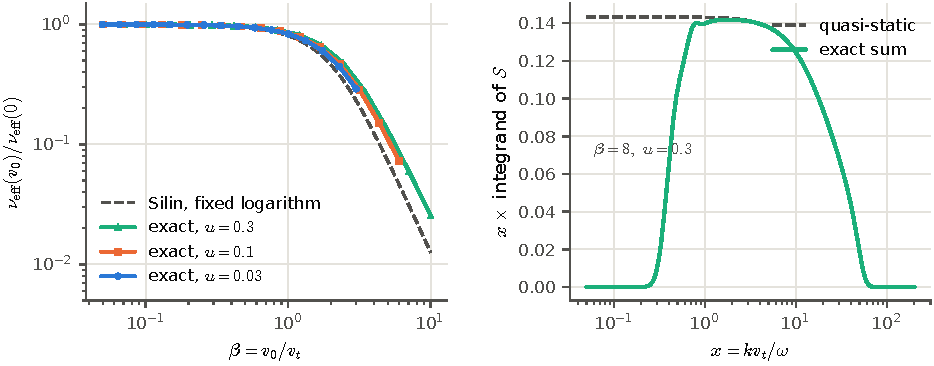
\includegraphics[width=\textwidth]{chapters/pd/fig_strong.pdf}
\caption{Strong fields. Left, the ratio $R=\nueff(v_0)/\nueff(0)$ of the exact
quantum heating rate of Eq.~\eqref{pd:eq:S-exact} for three photon energies,
and Silin's ratio $G$ at fixed logarithm, Eq.~\eqref{pd:eq:silin-Q}. Right, the
integrand of $\mathcal S$ times $x=kv_t/\omega$ at $\beta=8$, $u=0.3$, exact and in
the quasi-static limit of Eq.~\eqref{pd:eq:quasi-static}. The exact integrand is
cut off near $x\approx0.3$ by the thermal factor, and both are cut off near
$x\approx2\beta/u$ by the quantum limit on the momentum transfer.}
\label{pd:fig:strong}
\end{figure}


\section{The kinetic equation of an isotropic distribution}
\label{pd:sec:langdon}
This section returns to the master equation and follows the distribution of
the electrons, not only its energy. Let $F(v)$ be the isotropic velocity
distribution, $n_e=\int4\pi v^2F\,\dd v$, which is $2m^3f/(2\pi\hbar)^3$ in
terms of the occupation numbers.

\subsection{The averaged master equation for weak fields}
{\noindent}(1) For weak fields the master equation~\eqref{pd:eq:master} has the
terms $\ell=0,\pm1$. The term $\ell=0$ connects states of equal energy and
vanishes for an isotropic distribution. The field generates an anisotropy
proportional to $(\hat\pv\cdot\ehat)^2-\tfrac13$, which elastic collisions remove
faster than the field heats, and the isotropic part obeys the master equation
averaged over the direction of $\pv$,
\begin{equation}
\frac{\partial F(E)}{\partial t}=R_+(E)\big[F(E+\hbar\omega)-F(E)\big]+R_-(E)\big[F(E-\hbar\omega)-F(E)\big],
\end{equation}
where $R_\pm=n_iv\bar\sigma_{\pm1}$ with the cross sections of
Eq.~\eqref{pd:eq:sigma-iso},
\begin{equation}
\boxed{\;R_\pm(E)=\frac{2\pi}{3}\,\frac{n_iZ^2e^4a_0^2m}{\hbar^2p}\,L_\pm,\qquad
L_\pm=\ln\frac{p+p'_\pm}{|p-p'_\pm|},\qquad R_-(E)=0\;\;\text{for}\;\;E<\hbar\omega.\;}
\label{pd:eq:Rpm}
\end{equation}

{\noindent}(2) The density of states per unit energy and volume is
$g(E)=2\cdot4\pi p^2(2\pi\hbar)^{-3}\dd p/\dd E=8\pi mp/(2\pi\hbar)^3$, so
$g(E)R_+(E)$ is proportional to $L_+(p)$, which is symmetric in $p$ and
$p'_+$. Since $L_-$ at the momentum $p'_+$ is the same logarithm,
\begin{equation}
\boxed{\;g(E)\,R_+(E)=g(E+\hbar\omega)\,R_-(E+\hbar\omega).\;}
\label{pd:eq:db-rates}
\end{equation}
The upward rate from $E$ and the downward rate from $E+\hbar\omega$ are
balanced state by state, which is detailed balance for the rates.

\subsection{The flux form and the Fokker--Planck limit}
{\noindent}(1) Define the net flux of electrons per unit volume across the
step from $E$ to $E+\hbar\omega$,
\begin{equation}
\Phi(E)=g(E)R_+(E)\big[F(E)-F(E+\hbar\omega)\big].
\end{equation}
By Eq.~\eqref{pd:eq:db-rates} the averaged master equation is
\begin{equation}
g(E)\,\frac{\partial F(E)}{\partial t}=\Phi(E-\hbar\omega)-\Phi(E).
\end{equation}

{\noindent}(2) For $\hbar\omega\ll E$ expand,
$\Phi(E)\simeq-g R_+\hbar\omega\,\partial_EF$ and
$\Phi(E-\hbar\omega)-\Phi(E)\simeq-\hbar\omega\,\partial_E\Phi$, so
$g\,\partial_tF\simeq\partial_E[gR_+(\hbar\omega)^2\partial_EF]$. The product
$(\hbar\omega)^2R_+=\tfrac{2\pi}{3}n_iZ^2e^4v_0^2L/v$ stays finite as
$\hbar\omega\to0$, because $(\hbar\omega)^2a_0^2=\hbar^2v_0^2$.

{\noindent}(3) Change to the velocity, with $g\propto v$ and
$\partial_E=(mv)^{-1}\partial_v$,
\begin{equation}
\frac{\partial F}{\partial t}=\frac{2\pi n_iZ^2e^4v_0^2}{3m^2}\,\frac{1}{v^2}\,
\frac{\partial}{\partial v}\Big[\frac{L(v)}{v}\,\frac{\partial F}{\partial v}\Big].
\end{equation}
In terms of the momentum-transfer collision frequency
$\nu_m(v)=4\pi n_iZ^2e^4L(v)/m^2v^3$,
\begin{equation}
\boxed{\;\frac{\partial F}{\partial t}=\frac{1}{v^2}\,\frac{\partial}{\partial v}
\Big[v^2\,\frac{v_0^2}{6}\,\nu_m(v)\,\frac{\partial F}{\partial v}\Big],\qquad
\nu_m(v)=\frac{4\pi n_iZ^2e^4}{m^2v^3}\,L(v),\qquad L(v)=\ln\frac{2mv^2}{\hbar\omega}.\;}
\label{pd:eq:langdon}
\end{equation}
This is the inverse bremsstrahlung operator used by Langdon \cite{pd:Langdon1980}.
The quantum theory supplies its logarithm, $L=\ln(4E/\hbar\omega)$, which is the
limit $\hbar\omega\ll E$ of $\ln[(p+p'_+)/(p'_+-p)]$, the ratio of the largest
momentum transfer $2p$ to the smallest $\hbar\omega/v$.

\subsection{The heating rate of an arbitrary isotropic distribution}
{\noindent}(1) Multiply Eq.~\eqref{pd:eq:langdon} by $4\pi v^2\,mv^2/2$, integrate,
and integrate by parts once. With $C=2\pi n_iZ^2e^4v_0^2/3m^2$,
\begin{equation}
P=\int_0^\infty4\pi v^2\frac{mv^2}{2}\frac{\partial F}{\partial t}\dd v
=-4\pi mC\int_0^\infty L(v)\,\frac{\partial F}{\partial v}\,\dd v.
\end{equation}

{\noindent}(2) For a fixed logarithm the integral is $-LF(0)$, and
\begin{equation}
\boxed{\;P=4\pi mC\,L\,F(0).\;}
\label{pd:eq:F0}
\end{equation}
The absorption is proportional to the number of slow electrons, measured by
$F(0)$. For the Maxwellian $F(0)=n_e(2\pi v_t^2)^{-3/2}$, and
$P/(n_emv_0^2/2)=\nuT L$, which is Eq.~\eqref{pd:eq:Lambda-mb} with
$\Lambda\to L$.

{\noindent}(3) With the velocity-dependent logarithm and the Maxwellian,
$-\partial_vF=(v/v_t^2)F$, and $y=v^2/2v_t^2$ is exponentially distributed
under the weight $(v/v_t^2)e^{-v^2/2v_t^2}$. The average of
$L=\ln(4y/u)$ is $\ln(4/u)-\gamma$, which is Eq.~\eqref{pd:eq:Lambda-limits}. The
Fokker--Planck limit reproduces the exact Maxwellian result to first order in
$u$.

{\noindent}(4) The operator heats the slow electrons fastest, since
$v^2\nu_m\propto v^{-1}$. When this heating outpaces the electron--electron
collisions that restore the Maxwellian, the distribution becomes flat-topped
\cite{pd:Langdon1980}. For $F\propto\exp[-(v/v_m)^M]$ at fixed density and kinetic
energy, $v_m=v_t[3\Gamma(3/M)/\Gamma(5/M)]^{1/2}$ and
$F(0)=Mn_e/4\pi v_m^3\Gamma(3/M)$, so Eq.~\eqref{pd:eq:F0} at fixed $L$ gives the
ratio to the Maxwellian
\begin{equation}
\boxed{\;\frac{P_M}{P_2}=\frac{(2\pi)^{3/2}M}{4\pi\Gamma(3/M)}\Big[\frac{\Gamma(5/M)}{3\Gamma(3/M)}\Big]^{3/2}
=1,\;0.621,\;0.501,\;0.446\quad\text{for}\quad M=2,3,4,5,\;}
\label{pd:eq:superG}
\end{equation}
and $0.336$ for $M\to\infty$. This is consistent with the reduction by up to a
factor of two that Langdon reports \cite{pd:Langdon1980}.


\section{Summary}
\label{pd:sec:summary}
\noindent\textbf{In Summary:} An electron in the laser field is a Volkov
state, Eq.~\eqref{pd:eq:volkov}. Its matrix element with the ion potential is a
sum of harmonics weighted by $J_\ell(\kv\cdot\av)$, Eq.~\eqref{pd:eq:Vpp}, and
the golden rule gives the multiphoton cross section of Bunkin and Fedorov,
Eq.~\eqref{pd:eq:bf}. The operator method of the quantum Boltzmann equation paper
turns these rates into the master equation~\eqref{pd:eq:master} for the
occupation numbers, exactly at second order in the ion potential and without
Pauli blocking. Its energy moment is the heating rate, which in terms of the
Lindhard function is Eq.~\eqref{pd:eq:P-chi0}, and in the oscillating frame of
the interacting electron gas it becomes the dielectric form
Eq.~\eqref{pd:eq:P-silin}, with Dawson and Oberman for weak fields and Silin for
strong ones.

For weak fields and Maxwell electrons the collision frequency of the Drude
model is $\nuT\Lambda(u)$ with
$\Lambda(u)=[(1-e^{-u})/u]e^{u/2}K_0(u/2)$, which is
$\ln(4\kB T/e^\gamma\hbar\omega)$ for $\hbar\omega\ll\kB T$. The Coulomb
logarithm needs no cutoff. It is $\pi/\sqrt3$ times the thermally averaged
Born Gaunt factor, Eq.~\eqref{pd:eq:Lambda-gaunt}, Kirchhoff's law holds exactly,
and the frequency-integrated Gaunt factor is $2\sqrt3/\pi$. The degenerate
gas gives Ziman's formula, and every distribution has the same tail for
$\hbar\omega\gg\kB T$. Dynamic screening lowers the logarithm by $0.10$ at a
quarter of the critical density and by at most $0.56$ as $\omega\to\omega_p$,
Table~\ref{pd:tab:rpa}. In strong fields the
classical limit is Silin's $3Q(r)/r^3$, whose constant is
$\ln(4\sqrt2)+\gamma/2-1$, and the quantum result exceeds it because the
largest momentum transfer grows with the quiver velocity. For an isotropic
distribution the master equation reduces to Langdon's operator with the
quantum logarithm $\ln(2mv^2/\hbar\omega)$, Eq.~\eqref{pd:eq:langdon}.

Three corrections to the classical treatment of \cite{pd:Atzeni2004} follow,
Appendix~\ref{pd:app:atzeni}. The free--free and the Drude absorption
coefficients, Eqs.~(11.31) and (11.34)~\cite{pd:Atzeni2004}, differ by a factor of
$4.4$ as printed, and they agree only when the Gaunt factor is
$(\sqrt3/\pi)\ln\Lambda$. The current of Eq.~(11.8)~\cite{pd:Atzeni2004} carries
the wrong sign, which Eq.~(11.9)~\cite{pd:Atzeni2004} does not inherit. The constant of the
Coulomb logarithm of Eq.~(10.136)~\cite{pd:Atzeni2004} is $0.9$ below the value of
the cutoffs stated with it.

The theory has three limits that the next steps of this project should lift.
The Born approximation needs $Ze^2/\hbar v\ll1$, which fails for high $Z$ and
low temperature, where the exact Coulomb Gaunt factors of Sommerfeld
\cite{pd:Sommerfeld1931} and Karzas and Latter \cite{pd:KarzasLatter1961} and the
Elwert factor \cite{pd:Elwert1939} replace the Born ones \cite{pd:Moll2012}. The
random-phase response omits local-field corrections and the correlations of a
strongly coupled plasma. The anisotropy of the distribution and its relaxation
by electron--electron collisions, which decide when Langdon's flat-topped
distribution forms, require the full kinetic equation with both collision
terms.


\chapterappendix
\section{Reduction to Atzeni and Meyer-ter-Vehn}
\label{pd:app:atzeni}
This appendix takes the equations of \cite{pd:Atzeni2004} that bear on inverse
bremsstrahlung in turn, and states for each what the quantum theory gives.
Table~\ref{pd:tab:atzeni} collects the numbers, which the check script
recomputes from the constants of CODATA 2018.

\subsection{The Drude model, Eqs.~(11.7) to (11.12)}
Section~\ref{pd:sec:drude} derives Eqs.~(11.7), (11.9) and (11.12)~\cite{pd:Atzeni2004}.
The current of Eq.~(11.8)~\cite{pd:Atzeni2004} as printed is
$e^2n_0\Ev_1/[im_e(\omega+i\nu_e)]$, which equals $-\sigma\Ev_1$ with the
conductivity $\sigma$ of Eq.~\eqref{pd:eq:drude-sigma}. Inserted into
Eq.~(11.4)~\cite{pd:Atzeni2004} it would give $\varepsilon_T=1+\omega_p^2/\omega(\omega+i\nu)$,
the wrong sign of the plasma term. Eq.~(11.9)~\cite{pd:Atzeni2004} has the
correct sign, so the slip is confined to Eq.~(11.8). The quantum theory
replaces $\nu_e$ by $\nueff$ of Eq.~\eqref{pd:eq:nu-weak}.

\subsection{The collision time and the Coulomb logarithm, Eqs.~(10.133) and (10.136)}
\label{pd:app:atzeni-log}
{\noindent}(1) Eq.~(10.133)~\cite{pd:Atzeni2004} is $\tau_e=1/\nuT\ln\Lambda_e$ with
$\nuT$ of Eq.~\eqref{pd:eq:nuT}. Its numerical coefficient,
$1.088\times10^{-11}$~s, agrees with the printed $1.09\times10^{-11}$~s.

{\noindent}(2) Eq.~(10.136)~\cite{pd:Atzeni2004} prints
$\ln\Lambda_e=7.1-0.5\ln n_e+\ln T_e$. The text states that it is the
logarithm of $\lambda_D/\lambda_{\rm dB}$ with $\lambda_{\rm dB}=\hbar/2m_ev$ and
$m_ev^2/2=3\kB T_e/2$. At $\kB T_e=1$~keV and $n_e=10^{21}$~cm$^{-3}$ these
cutoffs give $\lambda_D=7.43\times10^{-7}$~cm, $\lambda_{\rm dB}=2.52\times10^{-10}$~cm and
$\ln(\lambda_D/\lambda_{\rm dB})=7.99$, so the printed constant is $0.89$ lower
than its stated definition.

{\noindent}(3) The quantum theory gives the logarithm of
Eq.~\eqref{pd:eq:Lambda-mb}, whose cutoffs are $v_t/\omega$ and
$0.445\hbar/mv_t$, Eq.~\eqref{pd:eq:cutoffs}, and Eq.~\eqref{pd:eq:Lambda-rpa} with
screening. Table~\ref{pd:tab:scales} compares them with Eq.~(10.136).

\subsection{The critical density and Eqs.~(11.30) to (11.33)}
{\noindent}(1) Eq.~(11.30)~\cite{pd:Atzeni2004} is $n_c=\pi m_ec^2/e^2\lambda_L^2=1.115\times10^{21}/\lambda_L^2$~cm$^{-3}$
with $\lambda_L$ in $\mu$m, printed as $1.1\times10^{21}$.

{\noindent}(2) Eq.~(11.33)~\cite{pd:Atzeni2004} prints
$\nu_{ec}/c\approx25Z_i/\lambda_L^2T_e^{3/2}$~cm$^{-1}$ for $\ln\Lambda_e\approx8$.
Equations (10.133) and (11.30)~\cite{pd:Atzeni2004} give $27.3$ for the same
logarithm.

{\noindent}(3) The text estimates $\ln\Lambda_e\approx8$ from Eq.~(10.136) for
$\kB T_e=1$~keV at the critical density of $\lambda_L=0.5~\mu$m,
$n_c=4.46\times10^{21}$~cm$^{-3}$. Eq.~(10.136) gives $6.35$ there and its stated
cutoffs $7.24$. The quantum theory gives $\Lambda(u)=6.81$ at
$u=\hbar\omega/\kB T=0.00248$ without screening.

\subsection{Kramers' cross section and the free--free opacity, Eqs.~(10.89) to (10.93)}
{\noindent}(1) The Maxwell average of Kramers' cross section,
Eq.~(10.89)~\cite{pd:Atzeni2004}, multiplied by $h\nu/4\pi Am_p$, is
\begin{equation}
\begin{aligned}
\eta_\nu&=\frac{h\nu}{4\pi Am_p}\,n_e\Big(\frac{m}{2\pi\kB T}\Big)^{3/2}4\pi\,
\frac{32\pi^2Z^2e^6}{3\sqrt3m^2c^3h\nu}\int_{v_{\min}}^\infty v\,e^{-mv^2/2\kB T}\dd v\\
&=\frac{16\pi}{3\sqrt{6\pi}}\,\frac{e^6Z^2n_e}{m^2c^3(\kB T/m)^{1/2}Am_p}\,e^{-h\nu/\kB T},
\end{aligned}
\end{equation}
which is Eq.~(10.91)~\cite{pd:Atzeni2004}. Kirchhoff's law with
$B_\nu=2h\nu^3c^{-2}e^{-h\nu/\kB T}$ for the true absorption gives
Eq.~(10.92)~\cite{pd:Atzeni2004} in its symbolic form. Its numerical form
evaluates to $2.74\,Z^3\rho/A^2T^{1/2}(h\nu)^3$~cm$^2$\,g$^{-1}$ against the
printed $2.78$, and Eq.~(10.93)~\cite{pd:Atzeni2004} to $1.74\times10^{17}$ against
the printed $1.76\times10^{17}$~W\,g$^{-1}$. The two differences are the same
$1.4$~percent.

{\noindent}(2) The Gaunt factor $g\approx2\sqrt3/\pi$ that the text applies to
Eq.~(10.93)~\cite{pd:Atzeni2004} is the power-averaged Born Gaunt factor of
Eq.~\eqref{pd:eq:gaunt-power}, exactly.

\subsection{The two absorption coefficients, Eqs.~(11.31) and (11.34)}
\label{pd:app:atzeni-ff}
{\noindent}(1) By Eq.~\eqref{pd:eq:kirchhoff} the net absorption coefficient of
Kramers' form with a Gaunt factor $g$ is
$K=(\nuT/c)(\omega_p^2/\omega^2)(\pi/\sqrt3)\,g\,[(1-e^{-u})/u]/n_r$. With $g=1$ this is
Eq.~(11.34)~\cite{pd:Atzeni2004}, exactly. The Drude form
Eq.~(11.31)~\cite{pd:Atzeni2004} is the same with $(\pi/\sqrt3)g(1-e^{-u})/u$
replaced by $\ln\Lambda_e$. Their ratio is
\begin{equation}
\frac{K_{(11.31)}}{K_{(11.34)}}=\frac{\ln\Lambda_e}{(\pi/\sqrt3)\,g\,(1-e^{-u})/u}.
\end{equation}

{\noindent}(2) At $\lambda_L=0.5~\mu$m and $\kB T=1$~keV, $u=0.00248$, and with
$g=1$ and $\ln\Lambda_e=8$ the ratio is $4.42$. The numerical forms give
$6.19$ and $27.3\,Z/\lambda_L^2T_e^{3/2}$~cm$^{-1}$ at $n_e=n_c$, the same
ratio. The statement below Eq.~(11.34)~\cite{pd:Atzeni2004}, that the two agree
within a few percent, holds only for $g=(\sqrt3/\pi)\ln\Lambda_e=4.4$.

{\noindent}(3) The quantum theory gives both at once. The Born Gaunt factor at
$u=0.00248$ is $\langle g\rangle=3.758$, and both forms become
$\nuT\Lambda(u)$ with $\Lambda=6.81$.

\subsection{The classical dielectric function, Eq.~(11.19)}
The classical limit of the Lindhard function of Maxwell electrons is
Eq.~(11.19)~\cite{pd:Atzeni2004}, Section~\ref{pd:sec:rpa} step~(2). Its imaginary
part is Eq.~\eqref{pd:eq:imchi-classical}.

\subsection{Bohr and Bethe, Eqs.~(11.72) to (11.74)}
For stopping, \cite{pd:Atzeni2004} takes the smaller of the classical
logarithm of Bohr and the quantum one of Bethe, Eq.~(11.74). The same choice
arises here. The quantum Coulomb logarithm of
Eq.~\eqref{pd:eq:Lambda-mb} is the Bethe-type result and holds for
$\eta=Ze^2/\hbar v_t\ll1$. For $\eta\gtrsim1$ the lower cutoff becomes the
classical distance $r_0=Ze^2/mv^2$ and the Born result overestimates the
absorption, which the exact Coulomb Gaunt factors correct.

\begin{table}[ht]
\centering
\caption{Equations of \cite{pd:Atzeni2004} on inverse bremsstrahlung, as
printed and as recomputed or derived here.}
\label{pd:tab:atzeni}
\begin{tabular}{L{2.1cm}L{4.5cm}L{4.5cm}L{3.3cm}}
\toprule
Equation & Printed & Recomputed or derived & Status\\
\midrule
(11.8) & $e^2n_0\Ev_1/[im_e(\omega+i\nu_e)]$ & $ie^2n_0\Ev_1/[m_e(\omega+i\nu_e)]$ & sign slip\\
(11.9), (11.12) & Drude $\varepsilon_T$ and $K$ & Eqs.~(\ref*{pd:eq:drude-eps}), (\ref*{pd:eq:drude-K}) & confirmed\\
(10.133) & $1.09\times10^{-11}$~s & $1.088\times10^{-11}$~s & confirmed\\
(10.136) & constant $7.1$ & $7.99$ from its cutoffs & constant low by $0.89$\\
(11.30) & $1.1\times10^{21}/\lambda_L^2$ & $1.115\times10^{21}/\lambda_L^2$ & confirmed\\
(11.33) & $25$ & $27.3$ & $9$~percent low\\
text, $\ln\Lambda_e\approx8$ & from (10.136) & $6.35$ from (10.136), $6.81$ quantum & inconsistent\\
(10.91) & symbolic form & Maxwell average of (10.89) & confirmed\\
(10.92) & $2.78$ & $2.74$ & $1.4$~percent\\
(10.93) & $1.76\times10^{17}$ & $1.74\times10^{17}$ & $1.4$~percent\\
$g\approx2\sqrt3/\pi$ & quoted for (10.93) & Born power average, Eq.~(\ref*{pd:eq:gaunt-power}) & exact\\
(11.31) vs (11.34) & agree within a few percent & ratio $4.42$ & needs $g=4.4$\\
(11.19) & classical $\varepsilon_L$ & classical limit of Lindhard & confirmed\\
\bottomrule
\end{tabular}
\end{table}


\section{Mathematical identities}
\label{pd:app:math}
\subsection{An integral of the error function}
Integrate by parts, $\int_0^S\erf(s)s^{-1}\dd s=\erf(S)\ln S-(2/\sqrt\pi)\int_0^Se^{-s^2}\ln s\,\dd s$.
Differentiating $\int_0^\infty s^{2a-1}e^{-s^2}\dd s=\Gamma(a)/2$ with respect to $a$
at $a=\tfrac12$ gives $\int_0^\infty e^{-s^2}\ln s\,\dd s=\Gamma'(\tfrac12)/4
=\tfrac{\sqrt\pi}{4}\psi(\tfrac12)=-\tfrac{\sqrt\pi}{4}(\gamma+2\ln2)$, with
$\psi(\tfrac12)=-\gamma-2\ln2$ from Eq.~(5.4.13)~\cite{pd:DLMF}. Since
$1-\erf S$ and the tail of the last integral decay faster than any power,
\begin{equation}
\int_0^S\frac{\erf s}{s}\,\dd s=\ln S+\frac\gamma2+\ln2+o(1).
\label{pd:eq:erf-integral}
\end{equation}

\subsection{A logarithmic integral}
With $x=\sin\varphi$,
\begin{equation}
\int_0^1\Big[\frac{1}{(1-x^2)^{1/2}}-1\Big]\frac{\dd x}{x}
=\int_0^{\pi/2}\frac{1-\cos\varphi}{\sin\varphi}\,\dd\varphi
=\int_0^{\pi/2}\tan\frac\varphi2\,\dd\varphi=\Big[-2\ln\cos\frac\varphi2\Big]_0^{\pi/2}=\ln2.
\label{pd:eq:ln2-integral}
\end{equation}

\subsection{The large-field limit of the phase average}
{\noindent}(1) With $s=s_0\sin\theta'$ and the symmetry of the average,
$\langle g(s_0\cos\theta)\rangle=(2/\pi)\int_0^{s_0}g(s)(s_0^2-s^2)^{-1/2}\dd s$.

{\noindent}(2) For the part $\sqrt\pi\erf(s)/s$ write
$(s_0^2-s^2)^{-1/2}=s_0^{-1}\{1+[(1-s^2/s_0^2)^{-1/2}-1]\}$. The first term gives
$s_0^{-1}\sqrt\pi[\ln s_0+\gamma/2+\ln2]$ by Eq.~\eqref{pd:eq:erf-integral}. In the
second term $\erf(s)\to1$ wherever the bracket is not small, and
Eq.~\eqref{pd:eq:ln2-integral} gives $s_0^{-1}\sqrt\pi\ln2$.

{\noindent}(3) The part $-2e^{-s^2}$ is confined to $s\lesssim1$, where
$(s_0^2-s^2)^{-1/2}\simeq s_0^{-1}$, and gives $-s_0^{-1}\sqrt\pi$.

{\noindent}(4) Adding, $\langle g\rangle=(2/\pi s_0)\sqrt\pi[\ln s_0+\gamma/2+2\ln2-1]
=(2/\sqrt\pi s_0)[\ln(4s_0)+\gamma/2-1]$, which is the form used in
Eq.~\eqref{pd:eq:G-limits}.

\subsection{The phase average of a Gaussian}
With $\cos^2\theta=\tfrac12(1+\cos2\theta)$ and Eq.~(10.32.1)~\cite{pd:DLMF},
$I_0(z)=\pi^{-1}\int_0^\pi e^{\pm z\cos\phi}\dd\phi$,
\begin{equation}
\big\langle e^{-a\cos^2\theta}\big\rangle_\theta=e^{-a/2}\big\langle e^{-(a/2)\cos2\theta}\big\rangle_\theta
=e^{-a/2}I_0\Big(\frac a2\Big).
\end{equation}


\section{The numerical checks}
\label{pd:app:checks}
A check script verifies every boxed
result of these notes, in their order, by an independent numerical route.
The routes are quadrature of the defining integrals in place of the closed
forms, finite differences in place of derivatives, the golden-rule time
integral at finite times, the cross-section route against the Lindhard route,
an exact computation in the Fock space of three fermion modes for the
equation of motion, and the published equations of
\cite{pd:BunkinFedorov1966,pd:Silin1965,pd:Atzeni2004} as printed. It runs
with \texttt{numpy} and \texttt{scipy} under Python~3 in about
fifteen seconds. Table~\ref{pd:tab:checks} is written by the script itself. A
quantitative check passes when its deviation is below the tolerance stated in
the script, which reflects the precision of the quadrature or of the
asymptotic expansion it tests. A printed number passes when the script
reproduces it to its last printed digit. The figures are made by a second script.

\begin{longtable}{L{4.0cm}cccc}
\caption{The numerical checks of these notes, by the equation, table or section they verify. The second column counts all checks of the row. The third gives the largest deviation among its quantitative checks, relative, or absolute for quantities near zero, and is empty when the row has none. The fourth counts the numbers printed in these notes that the script reproduces to their last printed digit, and the fifth the logical conditions, such as a sign or a monotone decrease.}\label{pd:tab:checks}\\
\toprule
Equation & Checks & Largest deviation & Printed & Logical\\
\midrule
\endfirsthead
\toprule
Equation & Checks & Largest deviation & Printed & Logical\\
\midrule
\endhead
\bottomrule
\endfoot
Eq.~(\ref*{pd:eq:drude-sigma}) & 2 & $1.3\times10^{-16}$ &  & \\
Eq.~(\ref*{pd:eq:drude-eps}) & 2 & $2.9\times10^{-16}$ &  & \\
Eq.~(\ref*{pd:eq:drude-imeps}) & 1 & $6.4\times10^{-16}$ &  & \\
Eq.~(\ref*{pd:eq:P-drude}) & 2 & $2.9\times10^{-11}$ &  & \\
Eq.~(\ref*{pd:eq:drude-K}) & 3 & $1.6\times10^{-7}$ &  & \\
Eq.~(\ref*{pd:eq:nuT}) & 1 &  & 1 & \\
Eq.~(\ref*{pd:eq:quiver}) & 3 & $1.6\times10^{-12}$ &  & \\
Eq.~(\ref*{pd:eq:alpha-A}) & 2 & $0$ &  & \\
Eq.~(\ref*{pd:eq:H-KH1}) & 2 & $1.9\times10^{-16}$ &  & \\
Eq.~(\ref*{pd:eq:vk}) & 3 & $1.8\times10^{-16}$ &  & \\
Eq.~(\ref*{pd:eq:volkov}) & 2 & $5.0\times10^{-13}$ &  & \\
Eq.~(\ref*{pd:eq:jacobi-anger}) & 3 & $4.6\times10^{-16}$ &  & \\
Eq.~(\ref*{pd:eq:bessel-sums}) & 9 & $5.6\times10^{-16}$ &  & \\
Eq.~(\ref*{pd:eq:bessel-genfun}) & 6 & $8.5\times10^{-15}$ &  & \\
Eq.~(\ref*{pd:eq:bessel-small}) & 2 & $2.5\times10^{-7}$ &  & \\
Eq.~(\ref*{pd:eq:Vpp}) & 2 & $1.2\times10^{-16}$ &  & \\
Eq.~(\ref*{pd:eq:rate}) & 2 & $1.1\times10^{-3}$ &  & \\
Eq.~(\ref*{pd:eq:rate-ions}) & 1 & $1.4\times10^{-3}$ &  & \\
Eq.~(\ref*{pd:eq:bf}) & 2 & $8.6\times10^{-8}$ &  & \\
Eq.~(\ref*{pd:eq:rutherford}) & 2 & $4.0\times10^{-16}$ &  & \\
Eq.~(\ref*{pd:eq:sigma-theta0}) & 3 & $6.1\times10^{-15}$ &  & \\
Eq.~(\ref*{pd:eq:sigma-iso}) & 3 & $2.0\times10^{-15}$ &  & \\
Eq.~(\ref*{pd:eq:bf10}) & 15 & $1.5\times10^{-6}$ &  & 1\\
Eq.~(\ref*{pd:eq:arcsine}) & 2 & $7.9\times10^{-6}$ &  & 1\\
Eq.~(\ref*{pd:eq:bilinear}) & 2 & $0$ &  & 1\\
Eq.~(\ref*{pd:eq:eom}) & 1 & $1.8\times10^{-16}$ &  & \\
Eq.~(\ref*{pd:eq:markov}) & 2 & $1.3\times10^{-11}$ &  & \\
Eq.~(\ref*{pd:eq:second-order}) & 1 & $3.0\times10^{-13}$ &  & \\
Eq.~(\ref*{pd:eq:no-blocking}) & 2 & $3.6\times10^{-16}$ &  & \\
Eq.~(\ref*{pd:eq:master}) & 1 & $1.4\times10^{-14}$ &  & \\
Eq.~(\ref*{pd:eq:P-general}) & 2 & $1.5\times10^{-15}$ &  & 1\\
Eq.~(\ref*{pd:eq:imchi-general}) & 3 & $3.7\times10^{-10}$ &  & \\
Eq.~(\ref*{pd:eq:imchi-mb}) & 3 & $3.3\times10^{-15}$ &  & \\
Eq.~(\ref*{pd:eq:imchi-fd}) & 6 & $2.3\times10^{-14}$ &  & \\
Eq.~(\ref*{pd:eq:imchi-classical}) & 4 & $7.0\times10^{-8}$ &  & 2\\
Eq.~(\ref*{pd:eq:K0-integral}) & 2 & $1.7\times10^{-15}$ &  & \\
Eq.~(\ref*{pd:eq:Lambda-mb}) & 10 & $6.8\times10^{-12}$ &  & \\
Eq.~(\ref*{pd:eq:Lambda-limits}) & 4 & $2.5\times10^{-3}$ &  & 2\\
Eq.~(\ref*{pd:eq:cutoffs}) & 4 &  & 4 & \\
Table~\ref*{pd:tab:Lambda} & 36 &  & 36 & \\
Eq.~(\ref*{pd:eq:nu-fd}) & 5 & $4.5\times10^{-6}$ &  & \\
Eq.~(\ref*{pd:eq:nu-T0}) & 8 & $2.4\times10^{-7}$ &  & \\
Eq.~(\ref*{pd:eq:L0-limits}) & 6 & $5.0\times10^{-4}$ &  & 2\\
Eq.~(\ref*{pd:eq:tail}) & 5 & $8.4\times10^{-5}$ &  & \\
Eq.~(\ref*{pd:eq:spont-stim}) & 1 & $1.1\times10^{-16}$ &  & \\
Eq.~(\ref*{pd:eq:spont-diff}) & 1 & $1.7\times10^{-15}$ &  & \\
Eq.~(\ref*{pd:eq:born-brems}) & 3 & $2.4\times10^{-12}$ &  & \\
Eq.~(\ref*{pd:eq:gaunt-born}) & 3 & $2.2\times10^{-16}$ &  & \\
Eq.~(\ref*{pd:eq:gaunt-avg}) & 4 & $3.5\times10^{-12}$ &  & \\
Eq.~(\ref*{pd:eq:Lambda-gaunt}) & 4 & $5.2\times10^{-15}$ &  & \\
Eq.~(\ref*{pd:eq:gaunt-power}) & 3 & $1.1\times10^{-13}$ & 1 & \\
Eq.~(\ref*{pd:eq:kirchhoff}) & 2 & $6.9\times10^{-16}$ &  & \\
Eq.~(\ref*{pd:eq:frames}) & 1 & $6.6\times10^{-16}$ &  & \\
Eq.~(\ref*{pd:eq:chi0-Z}) & 5 & $1.5\times10^{-11}$ &  & \\
Eq.~(\ref*{pd:eq:P-silin}) & 4 & $1.1\times10^{-15}$ &  & \\
Eq.~(\ref*{pd:eq:Lambda-rpa}) & 8 & $1.3\times10^{-3}$ &  & \\
Eq.~(\ref*{pd:eq:dawson-oberman}) & 1 & $3.1\times10^{-15}$ &  & \\
Table~\ref*{pd:tab:rpa} & 26 &  & 26 & \\
Eq.~(\ref*{pd:eq:Bl-recursion}) & 12 & $9.6\times10^{-16}$ &  & \\
Eq.~(\ref*{pd:eq:S-exact}) & 4 & $1.5\times10^{-5}$ &  & \\
Table~\ref*{pd:tab:strong} & 12 &  & 12 & \\
Eq.~(\ref*{pd:eq:quasi-static}) & 2 & $3.9\times10^{-5}$ &  & 1\\
Eq.~(\ref*{pd:eq:g-function}) & 7 & $8.7\times10^{-10}$ &  & \\
Eq.~(\ref*{pd:eq:silin-Q}) & 8 & $2.4\times10^{-14}$ &  & \\
Eq.~(\ref*{pd:eq:G}) & 1 & $4.5\times10^{-7}$ &  & \\
Eq.~(\ref*{pd:eq:G-limits}) & 6 & $1.0\times10^{-4}$ & 1 & \\
Eq.~(\ref*{pd:eq:db-rates}) & 3 & $0$ &  & \\
Eq.~(\ref*{pd:eq:Rpm}) & 3 & $0$ &  & \\
Eq.~(\ref*{pd:eq:langdon}) & 4 & $2.8\times10^{-8}$ &  & 2\\
Eq.~(\ref*{pd:eq:F0}) & 2 & $2.2\times10^{-13}$ &  & \\
Eq.~(\ref*{pd:eq:superG}) & 7 & $3.0\times10^{-16}$ & 5 & \\
Table~\ref*{pd:tab:atzeni} & 15 & $3.5\times10^{-8}$ & 13 & \\
Sec.~\ref*{pd:app:atzeni-log} & 4 &  & 4 & \\
Sec.~\ref*{pd:app:atzeni-ff} & 7 & $3.3\times10^{-16}$ & 5 & \\
Table~\ref*{pd:tab:scales} & 36 &  & 36 & \\
Sec.~\ref*{pd:sec:dipole} & 2 &  & 2 & \\
Sec.~\ref*{pd:sec:closed} & 2 &  & 2 & \\
Eq.~(\ref*{pd:eq:erf-integral}) & 2 & $1.8\times10^{-16}$ &  & \\
Eq.~(\ref*{pd:eq:ln2-integral}) & 1 & $4.5\times10^{-14}$ &  & \\
Sec.~\ref*{pd:app:math} & 6 & $7.1\times10^{-6}$ &  & \\
\midrule
Total & 394 & & 148 & 13\\
\end{longtable}



\begin{thebibliography}{99}

\bibitem{pd:Atzeni2004} S. Atzeni and J. Meyer-ter-Vehn, \emph{The Physics of
Inertial Fusion: Beam Plasma Interaction, Hydrodynamics, Hot Dense Matter}
(Oxford University Press, Oxford, 2004), doi:10.1093/acprof:oso/9780198562641.001.0001.

\bibitem{pd:Volkov1935} D. M. Wolkow, \"Uber eine Klasse von L\"osungen der
Diracschen Gleichung, Z. Phys. \textbf{94}, 250 (1935), doi:10.1007/BF01331022.

\bibitem{pd:BunkinFedorov1966} F. V. Bunkin and M. V. Fedorov, Bremsstrahlung in a
strong radiation field, Sov. Phys. JETP \textbf{22}, 844 (1966) [Zh. Eksp. Teor.
Fiz. \textbf{49}, 1215 (1965)].

\bibitem{pd:Watson2026} C. K. Watson, M. I. Shaukat, A. Svidzinsky, M. Kim, and M. O.
Scully, Unified microscopic foundations of the quantum Boltzmann equation,
Fluct. Noise Lett. \textbf{25}, 2640002 (2026), doi:10.1142/S021947752640002X.

\bibitem{pd:Watson2026erratum} C. K. Watson, M. I. Shaukat, A. Svidzinsky, M. Kim,
and M. O. Scully, Erratum: Unified microscopic foundations of the quantum
Boltzmann equation, manuscript (2026).

\bibitem{pd:DawsonOberman1962} J. Dawson and C. Oberman, High-frequency
conductivity and the emission and absorption coefficients of a fully ionized
plasma, Phys. Fluids \textbf{5}, 517 (1962), doi:10.1063/1.1706652.

\bibitem{pd:JohnstonDawson1973} T. W. Johnston and J. M. Dawson, Correct values for
high-frequency power absorption by inverse bremsstrahlung in plasmas, Phys.
Fluids \textbf{16}, 722 (1973), doi:10.1063/1.1694419.

\bibitem{pd:Kramers1923} H. A. Kramers, On the theory of X-ray absorption and of
the continuous X-ray spectrum, Phil. Mag. \textbf{46}, 836 (1923),
doi:10.1080/14786442308565244.

\bibitem{pd:Silin1965} V. P. Silin, Nonlinear high-frequency plasma conductivity,
Sov. Phys. JETP \textbf{20}, 1510 (1965) [Zh. Eksp. Teor. Fiz. \textbf{47}, 2254
(1964)].

\bibitem{pd:Lindhard1954} J. Lindhard, On the properties of a gas of charged
particles, Kgl. Danske Vid. Selsk. Mat.-Fys. Medd. \textbf{28}, No.~8 (1954).

\bibitem{pd:DLMF} F. W. J. Olver \emph{et al.}, eds., \emph{NIST Digital Library of
Mathematical Functions}, https://dlmf.nist.gov, Chapters 5 and 10.

\bibitem{pd:Henneberger1968} W. C. Henneberger, Perturbation method for atoms in
intense light beams, Phys. Rev. Lett. \textbf{21}, 838 (1968),
doi:10.1103/PhysRevLett.21.838.

\bibitem{pd:Marcuse1962} D. Marcuse, Stimulated emission of bremsstrahlung, Bell
Syst. Tech. J. \textbf{41}, 1557 (1962), doi:10.1002/j.1538-7305.1962.tb03994.x.

\bibitem{pd:Kohn1961} W. Kohn, Cyclotron resonance and de Haas--van Alphen
oscillations of an interacting electron gas, Phys. Rev. \textbf{123}, 1242
(1961), doi:10.1103/PhysRev.123.1242.

\bibitem{pd:GiulianiVignale2005} G. F. Giuliani and G. Vignale, \emph{Quantum Theory
of the Electron Liquid} (Cambridge University Press, Cambridge, 2005),
doi:10.1017/CBO9780511619915.

\bibitem{pd:KullPlagne2001} H.-J. Kull and L. Plagne, Quantum-mechanical
dielectric model of the electron--ion collision frequency in strong laser
fields, Phys. Plasmas \textbf{8}, 5244 (2001), doi:10.1063/1.1416182.

\bibitem{pd:Bornath2001} Th. Bornath, M. Schlanges, P. Hilse, and D. Kremp,
Nonlinear collisional absorption in dense laser plasmas, Phys. Rev. E
\textbf{64}, 026414 (2001), doi:10.1103/PhysRevE.64.026414.

\bibitem{pd:Kremp1999} D. Kremp, Th. Bornath, M. Bonitz, and M. Schlanges, Quantum
kinetic theory of plasmas in strong laser fields, Phys. Rev. E \textbf{60},
4725 (1999), doi:10.1103/PhysRevE.60.4725.

\bibitem{pd:FriedConte1961} B. D. Fried and S. D. Conte, \emph{The Plasma
Dispersion Function} (Academic Press, New York, 1961).

\bibitem{pd:Langdon1980} A. B. Langdon, Nonlinear inverse bremsstrahlung and
heated-electron distributions, Phys. Rev. Lett. \textbf{44}, 575 (1980),
doi:10.1103/PhysRevLett.44.575.

\bibitem{pd:Sommerfeld1931} A. Sommerfeld, \"Uber die Beugung und Bremsung der
Elektronen, Ann. Phys. \textbf{403}, 257 (1931), doi:10.1002/andp.19314030302.

\bibitem{pd:KarzasLatter1961} W. J. Karzas and R. Latter, Electron radiative
transitions in a Coulomb field, Astrophys. J. Suppl. \textbf{6}, 167 (1961),
doi:10.1086/190063.

\bibitem{pd:Elwert1939} G. Elwert, Versch\"arfte Berechnung von Intensit\"at und
Polarisation im kontinuierlichen R\"ontgenspektrum, Ann. Phys. \textbf{426},
178 (1939), doi:10.1002/andp.19394260206.

\bibitem{pd:Moll2012} M. Moll, M. Schlanges, Th. Bornath, and V. P. Krainov,
Inverse bremsstrahlung heating beyond the first Born approximation for dense
plasmas in laser fields, New J. Phys. \textbf{14}, 065010 (2012),
doi:10.1088/1367-2630/14/6/065010.

\end{thebibliography}
\endgroup

% Chapter ea: the note of October 20, 2026, assembled for the compendium -- do not edit by hand
\chapter{Detailed derivation of free--free absorption by electron--atom collisions at terahertz frequencies}\label{ea:chapter}
\notedate{October 20, 2026}
\begingroup
\noindent\emph{These notes derive, with every intermediate result written
out, the rate at which an electromagnetic wave of terahertz frequency is
absorbed by free electrons that collide with neutral atoms. They ask whether
the classical absorption kernel, the Lorentz-gas conductivity built on the
momentum-transfer cross section, is accurate at the terahertz frequencies
proposed for reheating the electrons of an electron-beam-pumped KrF laser
gas. The electron is described by exact scattering states of a local
potential that represents the atom, the field is treated to first order, and
the rate follows from the golden rule. Every boxed result is checked
numerically, as Appendix~\ref{ea:app:checks} describes.}

\medskip
\noindent For notation, Gaussian units are used. The
electron has charge $-e$ and mass $m$, and the atom is infinitely heavy and
sits at the origin. A state of momentum $\hbar\kv$ has energy
$E=\hbar^2k^2/2m$ and speed $v=\hbar k/m$. The wave is uniform and linearly
polarized along the unit vector $\ehat$, with amplitude $E_0$ and angular
frequency $\omega$, and $f=\omega/2\pi$ is its frequency. The absorption of one
photon takes the electron from $\hbar\kv$ to $\hbar\kv'$ with
$k'^2=k^2+2m\omega/\hbar$. The temperature of a Maxwell distribution is $T$ and
$u=\hbar\omega/\kB T$. The momentum-transfer cross section is $\sm(E)$, and a
cross section with a subscript $+$ or $-$ is the free--free cross section for
absorption or stimulated emission per unit photon flux, defined in
Sec.~\ref{ea:sec:cross}. The numbers are computed in atomic units, $\hbar=m=e=1$,
with the bohr $a_0$ and the hartree $E_h=27.211$~eV. A boxed equation is a
result that is checked.


\section{Why the atoms matter}
\label{ea:sec:why}

{\noindent}(1) Inverse bremsstrahlung, the absorption of a wave by electrons
that scatter on ions, heats laser plasmas \cite{ea:Atzeni2004}. In the gas of an electron-beam-pumped
KrF laser the electron density is $10^{19}$ to $2.7\times10^{21}$~m$^{-3}$
against an atom density of $2.4\times10^{25}$ to $4.9\times10^{25}$~m$^{-3}$,
so that there are $9\times10^3$ to $5\times10^6$ atoms for every ion. The
Coulomb cross section is larger by orders of magnitude, however, and
Sec.~\ref{ea:sec:ei} finds the regime in which each kind of collision dominates
the absorption. Away from the coldest and densest afterglow the atoms win.

{\noindent}(2) Free--free absorption on neutral atoms has been computed from
phase shifts for the negative hydrogen ion \cite{ea:OhmuraOhmura1960} and for
other atoms \cite{ea:Geltman1973}, and with the multichannel R-matrix method for
argon \cite{ea:BellBerrington1987}. Its inverse, the neutral bremsstrahlung, has
been measured \cite{ea:TaylorCaledonia1969,ea:Ranson1977} and explains part of the
electroluminescence of two-phase argon detectors \cite{ea:Buzulutskov2018}.

{\noindent}(3) Proposals to reheat the electrons of the laser gas with a
terahertz wave compute its absorption length with the classical kernel of the
Lorentz gas. That kernel is the
conductivity of electrons that scatter off heavy atoms with the energy
dependent collision frequency $\nu(v)=N\sm(v)v$, derived in
Sec.~\ref{ea:sec:classical}. It treats the electron as a classical particle that
absorbs energy continuously. Two quantum effects are missing from it. The
first is the ratio $u=\hbar\omega/\kB T$, which is $0.16$ at 1~THz and $4.5$
at the 28.3~THz of a CO$_2$ laser for electrons at the gas temperature of
300~K. The second is the structure of $\sm(E)$. Argon and krypton have a
Ramsauer--Townsend window in which $\sm$ falls from its value at 1~meV by a
factor of 82 in argon and 330 in krypton, to minima at 0.25 and 0.51~eV in the
LXCat sets, and a photon of 28.3~THz carries 0.117~eV. Table~\ref{ea:tab:scales}
lists the photon energy and $u$ at the frequencies used below.

\begin{table}[ht]
\caption{Photon energy $\hbar\omega$, the ratio $u=\hbar\omega/\kB T$ and the
stimulated-emission factor $(1-e^{-u})/u$ at 300~K, and $u$ for electrons at
0.63~eV.}
\label{ea:tab:scales}
\begin{center}
\begin{tabular}{lcccc}
\toprule
$f$ (THz) & $\hbar\omega$ (meV) & $u$, 300~K & $(1-e^{-u})/u$, 300~K & $u$, 0.63~eV\\
\midrule
\tabinput{chapters/ea/tab_scales.tex}
\bottomrule
\end{tabular}
\end{center}
\end{table}

{\noindent}(4) The question is the error of the classical kernel at 3 to
28~THz in two fills of the laser gas, Ne/Kr/F$_2$ = 0.948/0.05/0.002 at
2~atm and Ar/Kr/F$_2$ = 0.597/0.40/0.003 at 1~atm. The kernel is good enough
if the error is below 5\,\% in the band of 0.3 to 4~THz proposed for reheating.
Sections~\ref{ea:sec:ham} to~\ref{ea:sec:detailed} derive the quantum free--free
cross section of one electron and one atom exactly within a one-body model.
Section~\ref{ea:sec:soft} finds its soft-photon and classical limits, and
Sec.~\ref{ea:sec:exact} two limits in which it is known in closed form at any
photon energy. Sections~\ref{ea:sec:models} and~\ref{ea:sec:thermal} evaluate it for
model potentials fitted to the measured cross sections of neon, argon and
krypton. The answer is in Sec.~\ref{ea:sec:thermal} and in the Summary.

\section{The Hamiltonian}
\label{ea:sec:ham}

\subsection{One electron and one atom}
{\noindent}(1) The atom is represented by a local central potential $V(r)$
that acts on the scattering electron,
\begin{equation}
H_0=\frac{p^2}{2m}+V(r),\qquad
V(r)\to-\frac{\alpha_de^2}{2r^4}\quad(r\to\infty),
\label{ea:eq:H0}
\end{equation}
where $\alpha_d$ is the static dipole polarizability of the atom. At short
range $V$ contains the screened attraction of the nucleus and the repulsion
that the Pauli principle produces. In the one-body model the latter appears
because the occupied orbitals of the atom are bound states of the same
potential, so that the scattering states are orthogonal to them. The models
of Sec.~\ref{ea:sec:models} are of this kind.

{\noindent}(2) The atom is infinitely heavy. Its recoil changes the electron
energy by a fraction of order $m/M$, which is $1.4\times10^{-5}$ for argon,
and is neglected. Exchange between the scattering electron and the atomic
electrons, and the excitation of the atom, are outside the model. The second
needs at least 11.5~eV in argon and 9.9~eV in krypton and is closed for the
electrons that absorb terahertz photons.

\subsection{The wave}
{\noindent}(1) The wave has the field $\Ev(t)=E_0\ehat\cos\omega t$. At 1~THz
its wavelength is 0.3~mm and at 28.3~THz it is 10.6~$\mu$m. A collision takes
place within a few hundred $a_0$ of the atom, so the field is uniform over it
and the dipole approximation holds. In the length gauge the potential energy of
the charge $-e$ in the field is $e\Ev(t)\cdot\rv$, and
\begin{equation}
H(t)=H_0+eE_0\cos(\omega t)\,\ehat\cdot\rv
=H_0+\frac{eE_0}{2}\,\ehat\cdot\rv\,\big(e^{-i\omega t}+e^{i\omega t}\big).
\label{ea:eq:H}
\end{equation}
The term with $e^{-i\omega t}$ absorbs a photon and the term with
$e^{i\omega t}$ emits one.

{\noindent}(2) The field is weak when the quiver amplitude
$a=eE_0/m\omega^2$ is small against the wavelength of the electron. The
criterion and its numbers are in Sec.~\ref{ea:sec:strong}. In the weak field the
golden rule to first order in $E_0$ describes the absorption of one photon.

\subsection{The response of the atom to the wave}
\label{ea:sec:pb}
{\noindent}(1) The wave also polarizes the atom. Its induced dipole is
$\alpha_d\Ev(t)$, since $\hbar\omega$ is far below the excitation energies of
the atom. The electrostatic potential of a dipole $\mathbf d$ at the origin is
$\mathbf d\cdot\rv/r^3$, so the electron acquires the potential energy
$-e\alpha_d\Ev(t)\cdot\rv/r^3$. Together with Eq.~\eqref{ea:eq:H} the
interaction with the wave becomes
\begin{equation}
e\Ev(t)\cdot\rv\Big(1-\frac{\alpha_d}{r^3}\Big).
\label{ea:eq:pb-op}
\end{equation}
The second term is the polarization bremsstrahlung of the atom, the photon
absorbed through the dipole of the atom rather than through the electron.
Inside the atom the field of the dipole is screened, so the term is cut off
there. Section~\ref{ea:sec:pbnum} computes its effect with the same cut-off as the
polarization potential, and finds it below 0.7\,\% up to 3~THz. Until then it
is left out.

\section{The golden-rule cross section between exact scattering states}
\label{ea:sec:cross}

\subsection{The scattering states}
{\noindent}(1) The scattering states of $H_0$ with energy $E=\hbar^2k^2/2m$
are normalized to $\langle\psi_{\kv}|\psi_{\kv'}\rangle=\delta^3(\kv-\kv')$.
In partial waves,
\begin{equation}
\psi^{(\pm)}_{\kv}(\rv)=(2\pi)^{-3/2}\sum_{l=0}^\infty(2l+1)\,i^l
e^{\pm i\delta_l}\,\frac{u_{kl}(r)}{kr}\,P_l(\hat\kv\cdot\hat\rv),
\label{ea:eq:pw}
\end{equation}
where $u_{kl}$ is the real regular solution of the radial equation
\begin{equation}
u_{kl}''+\Big[k^2-U(r)-\frac{l(l+1)}{r^2}\Big]u_{kl}=0,\qquad
U(r)=\frac{2mV(r)}{\hbar^2},
\label{ea:eq:radial}
\end{equation}
normalized to unit amplitude,
$u_{kl}\to\sin(kr-l\pi/2+\delta_l)$ as $r\to\infty$, and $\delta_l(k)$ is
the phase shift. For $V=0$ the radial function is the Riccati--Bessel
function $\hat\jmath_l(kr)=kr\,j_l(kr)$, and Eq.~\eqref{ea:eq:pw} is the
expansion of the plane wave $(2\pi)^{-3/2}e^{i\kv\cdot\rv}$. The state
$\psi^{(+)}$ has an outgoing scattered wave and is the initial state. The
state $\psi^{(-)}$, with an incoming scattered wave, is the final state of an
electron detected in the direction $\hat\kv'$.

{\noindent}(2) With $P_l(\hat\kv\cdot\hat\rv)=\frac{4\pi}{2l+1}\sum_m
Y^*_{lm}(\hat\kv)Y_{lm}(\hat\rv)$,
\begin{equation}
\psi^{(\pm)}_{\kv}(\rv)=(2\pi)^{-3/2}\,\frac{4\pi}{kr}\sum_{lm}i^le^{\pm i\delta_l}
u_{kl}(r)\,Y^*_{lm}(\hat\kv)\,Y_{lm}(\hat\rv).
\label{ea:eq:pw-ylm}
\end{equation}

\subsection{The matrix element}
{\noindent}(1) The absorption term of Eq.~\eqref{ea:eq:H} has the matrix element
$(eE_0/2)M$ with $M=\langle\psi^{(-)}_{\kv'}|\ehat\cdot\rv|\psi^{(+)}_{\kv}\rangle$.
The complex conjugate of Eq.~\eqref{ea:eq:pw-ylm} for the final state has the
factors $(-i)^{l'}e^{+i\delta'_{l'}}Y_{l'm'}(\hat\kv')Y^*_{l'm'}(\hat\rv)$,
with $\delta'_{l'}=\delta_{l'}(k')$. The factor $r^2$ of $\dd^3r$ cancels the
two factors $1/r$, and
\begin{equation}
M=\frac{(4\pi)^2}{(2\pi)^3kk'}\sum_{lm,l'm'}(-i)^{l'}i^l
e^{i(\delta_l+\delta'_{l'})}\,Y_{l'm'}(\hat\kv')Y^*_{lm}(\hat\kv)\,
\langle l'm'|\ehat\cdot\hat\rv|lm\rangle\,R_{l\to l'},
\label{ea:eq:M}
\end{equation}
with the angular matrix element
$\langle l'm'|\ehat\cdot\hat\rv|lm\rangle=\int Y^*_{l'm'}\,\ehat\cdot\hat\rv\,
Y_{lm}\,\dd\Omega$ and the radial integral
\begin{equation}
R_{l\to l'}=\int_0^\infty u_{k'l'}(r)\,r\,u_{kl}(r)\,\dd r .
\label{ea:eq:Rlen}
\end{equation}
The integrand grows like $r$ at large $r$, and $R_{l\to l'}$ is defined with
the convergence factor $e^{-\eta r}$ and $\eta\to0^+$. Section~\ref{ea:sec:forms}
replaces it by an absolutely convergent integral.

{\noindent}(2) The angular matrix element vanishes unless $l'=l\pm1$, the
dipole selection rule. Appendix~\ref{ea:app:angular} sums its square over $m$
and $m'$,
\begin{equation}
\sum_{mm'}|\langle l+1,m'|\ehat\cdot\hat\rv|lm\rangle|^2=\frac{l+1}{3},\qquad
\sum_{mm'}|\langle l-1,m'|\ehat\cdot\hat\rv|lm\rangle|^2=\frac l3 .
\label{ea:eq:angsum}
\end{equation}

\subsection{The rate and its average over directions}
{\noindent}(1) The golden rule gives the rate of absorption from the state
$\psi^{(+)}_{\kv}$ into all final directions,
\begin{equation}
W_+=\frac{2\pi}{\hbar}\Big(\frac{eE_0}{2}\Big)^2\int\dd^3k'\,|M|^2\,
\delta\Big(\frac{\hbar^2k'^2}{2m}-\frac{\hbar^2k^2}{2m}-\hbar\omega\Big).
\end{equation}

{\noindent}(2) The electrons of a gas move in all directions, so $W_+$ is
averaged over $\hat\kv$. The integral over $\hat\kv'$ and the average over
$\hat\kv$ use the orthonormality of the $Y_{lm}$,
$\int Y_{l'm'}(\hat\kv')Y^*_{l''m''}(\hat\kv')\dd\Omega'=\delta_{l'l''}\delta_{m'm''}$
and $\frac1{4\pi}\int Y^*_{lm}(\hat\kv)Y_{\tilde l\tilde m}(\hat\kv)\dd\Omega
=\delta_{l\tilde l}\delta_{m\tilde m}/4\pi$. The cross terms between different
pairs $(l,l')$ vanish, the phases drop out, and with Eq.~\eqref{ea:eq:angsum}
\begin{equation}
\frac1{4\pi}\int\dd\Omega\int\dd\Omega'\,|M|^2
=\frac{(4\pi)^4}{(2\pi)^6k^2k'^2}\,\frac1{4\pi}\,\frac{S}{3}
=\frac{S}{3\pi^3k^2k'^2},
\label{ea:eq:Mavg}
\end{equation}
\begin{equation}
S=\sum_{l=0}^\infty\Big[(l+1)\,R_{l\to l+1}^2+l\,R_{l\to l-1}^2\Big].
\label{ea:eq:S}
\end{equation}

{\noindent}(3) The energy delta function contributes
$\int k'^2\dd k'\,\delta(\hbar^2k'^2/2m-E-\hbar\omega)=mk'/\hbar^2$. The
averaged rate is
\begin{equation}
\langle W_+\rangle=\frac{2\pi}{\hbar}\,\frac{e^2E_0^2}{4}\,\frac{mk'}{\hbar^2}\,
\frac{S}{3\pi^3k^2k'^2}=\frac{e^2E_0^2\,m\,S}{6\pi^2\hbar^3k^2k'} .
\end{equation}

\subsection{The cross section per photon flux}
{\noindent}(1) The state $\psi^{(+)}_{\kv}$ carries the incident flux
$(2\pi)^{-3}\hbar k/m$ of electrons, and the wave carries the flux
$\Phi=I/\hbar\omega$ of photons with $I=cE_0^2/8\pi$. The free--free cross
section for absorption is the rate divided by both fluxes,
$\sigma_+=\langle W_+\rangle/[(2\pi)^{-3}(\hbar k/m)\Phi]$. With
$(2\pi)^3\cdot8\pi/6\pi^2=32\pi^2/3$,
\begin{equation}
\boxed{\;\sigma_+(k\to k')=\frac{32\pi^2}{3}\,\frac{e^2m^2\omega}{\hbar^3c}\,
\frac{S}{k^3k'},\qquad \hbar k'=(\hbar^2k^2+2m\hbar\omega)^{1/2}.\;}
\label{ea:eq:sigplus}
\end{equation}
It has the dimension length$^4\times$time. An electron of speed $v$ among $N$
atoms per unit volume, in the photon flux $\Phi$, absorbs at the rate
$N\Phi v\sigma_+$.

{\noindent}(2) In the first Born approximation the radial functions are
$\hat\jmath_l$ and Eq.~\eqref{ea:eq:sigplus} must equal the one-photon limit of
the cross section of Bunkin and Fedorov \cite{ea:BunkinFedorov1966}, with
$J_1^2(x)\simeq x^2/4$, divided by $\Phi$. The check script compares the two
for a Gaussian potential and finds agreement to $10^{-14}$, which tests the
factor $32\pi^2/3$ and the angular sums together.

\subsection{Length, velocity and acceleration forms}
\label{ea:sec:forms}
{\noindent}(1) For eigenstates of $H_0$ the commutators
$[H_0,\rv]=-i\hbar\pv/m$ and $[H_0,\pv]=i\hbar\nabla V$ give
$[H_0,[H_0,\rv]]=(\hbar^2/m)\nabla V$. Between states that differ in energy by
$\hbar\omega$ the double commutator is $(\hbar\omega)^2$ times the matrix
element of $\rv$, so
\begin{equation}
\langle f|\rv|i\rangle=\frac{-i}{m\omega}\langle f|\pv|i\rangle
=\frac{1}{m\omega^2}\langle f|\nabla V|i\rangle .
\label{ea:eq:forms}
\end{equation}
For scattering states the boundary terms at infinity oscillate and vanish with
the convergence factor $e^{-\eta r}$, so the identities hold for the
regularized integrals of Eq.~\eqref{ea:eq:Rlen}.

{\noindent}(2) Since $\nabla V=V'(r)\hat\rv$ has the same angular structure as
$\rv=r\hat\rv$, the identity holds partial wave by partial wave,
\begin{equation}
\boxed{\;R_{l\to l'}=\frac{1}{m\omega^2}\int_0^\infty u_{k'l'}(r)\,V'(r)\,u_{kl}(r)\,\dd r .\;}
\label{ea:eq:Racc}
\end{equation}
The acceleration form converges absolutely when $V'$ falls faster than $1/r$,
as the $r^{-5}$ of the polarization tail does, and the numerics use it. The
form makes plain that the photon is absorbed where the electron is
accelerated, near the atom. The check script verifies Eq.~\eqref{ea:eq:Racc}
against the closed form of the length integral in the zero-range limit of
Sec.~\ref{ea:sec:zerorange}.

\section{Emission, detailed balance and the absorption coefficient}
\label{ea:sec:detailed}

\subsection{Stimulated emission and detailed balance}
{\noindent}(1) The term with $e^{i\omega t}$ in Eq.~\eqref{ea:eq:H} takes an
electron from $\hbar\kv'$ to $\hbar\kv$ and adds a photon to the wave. The
same steps give its cross section per photon flux, with $k$ and $k'$
exchanged in the prefactor,
$\sigma_-(k'\to k)=(32\pi^2e^2m^2\omega/3\hbar^3c)\,S'/(k'^3k)$. Here $S'$ has
the radial integrals $R'_{l\to l'}=\int u_{kl'}\,r\,u_{k'l}\,\dd r=R_{l'\to l}$.
Shifting the summation index in each of the two sums of Eq.~\eqref{ea:eq:S}
shows $S'=S$. Hence
\begin{equation}
\boxed{\;k^2\,\sigma_+(k\to k')=k'^2\,\sigma_-(k'\to k).\;}
\label{ea:eq:db}
\end{equation}
This is the principle of detailed balance for free--free transitions.

\subsection{The absorption coefficient}
{\noindent}(1) Let $g(E)\dd E$ be the fraction of electrons with energy in
$\dd E$, for an isotropic distribution normalized to $\int g\,\dd E=1$, and
let $\sigma_-(E)$ denote the emission cross section from $E$ to $E-\hbar\omega$,
zero for $E<\hbar\omega$. The wave loses photons at the rate
$n_eN\Phi\int g\,v(\sigma_+-\sigma_-)\dd E$ per unit volume, so its intensity
decays with the coefficient
\begin{equation}
\boxed{\;\kappa=n_eN\int_0^\infty g(E)\,v(E)\big[\sigma_+(E)-\sigma_-(E)\big]\dd E .\;}
\label{ea:eq:kappa-gen}
\end{equation}

{\noindent}(2) Shift the emission integral to $E=E''+\hbar\omega$ and use
Eq.~\eqref{ea:eq:db}, $\sigma_-(E''+\hbar\omega)=[E''/(E''+\hbar\omega)]\,\sigma_+(E'')$.
For the Maxwell distribution
$g(E)=2\pi^{-1/2}(\kB T)^{-3/2}E^{1/2}e^{-E/\kB T}$,
\begin{equation}
g(E''+\hbar\omega)\,v(E''+\hbar\omega)\,\frac{E''}{E''+\hbar\omega}
=e^{-u}\,g(E'')\,v(E''),
\end{equation}
since $g\,v$ is proportional to $E\,e^{-E/\kB T}$. Therefore
\begin{equation}
\boxed{\;\kappa=n_eN\,(1-e^{-u})\int_0^\infty g(E)\,v(E)\,\sigma_+(E)\,\dd E
\qquad\text{(Maxwell electrons)}.\;}
\label{ea:eq:kappa-mb}
\end{equation}
Stimulated emission reduces the absorption by the factor $1-e^{-u}$, as it
does for ions \cite{ea:KarzasLatter1961}.

\subsection{The kinetic equation and its Fokker--Planck limit}
\label{ea:sec:kinetic}
{\noindent}(1) Let $n(E)\dd E$ be the number of electrons per unit volume in
$\dd E$, and write $n=n_eE^{1/2}F(E)$ with $\int E^{1/2}F\,\dd E=1$, the
normalization of the two-term Boltzmann codes \cite{ea:HagelaarPitchford2005}.
An electron at $E$ climbs to $E+\hbar\omega$ at the rate
$W_+(E)=N\Phi v\sigma_+(E)$ and falls to $E-\hbar\omega$ at the rate
$W_-(E)=N\Phi v\sigma_-(E)$. The master equation for the distribution is
\begin{equation}
\frac{\partial n(E)}{\partial t}=W_+(E-\hbar\omega)n(E-\hbar\omega)
+W_-(E+\hbar\omega)n(E+\hbar\omega)-\big[W_+(E)+W_-(E)\big]n(E).
\label{ea:eq:master}
\end{equation}

{\noindent}(2) Detailed balance, Eq.~\eqref{ea:eq:db}, makes the two rates that
connect $E$ and $E+\hbar\omega$ equal after weighting with $E^{1/2}$,
\begin{equation}
W_+(E)\,E^{1/2}=W_-(E+\hbar\omega)\,(E+\hbar\omega)^{1/2}
=N\Phi\Big(\frac2m\Big)^{1/2}E\,\sigma_+(E)\equiv\mathcal Q\Big(E+\frac{\hbar\omega}2\Big).
\end{equation}
Dividing Eq.~\eqref{ea:eq:master} by $n_e$ gives the jump operator in
conservation form,
\begin{equation}
\boxed{\;\frac{\partial(E^{1/2}F)}{\partial t}
=\mathcal Q\Big(E+\frac{\hbar\omega}2\Big)\big[F(E+\hbar\omega)-F(E)\big]
-\mathcal Q\Big(E-\frac{\hbar\omega}2\Big)\big[F(E)-F(E-\hbar\omega)\big].\;}
\label{ea:eq:jump}
\end{equation}
The right side is a difference of two fluxes through the energies
$E\pm\hbar\omega/2$, so the operator conserves the number of electrons.

{\noindent}(3) When $\hbar\omega$ is small against the scale on which $F$ and
$\mathcal Q$ vary, each bracket is $\hbar\omega\,\partial F/\partial E$ at the
midpoint, and the difference of the two fluxes is $\hbar\omega$ times their
derivative,
\begin{equation}
\frac{\partial(E^{1/2}F)}{\partial t}=\frac{\partial}{\partial E}
\Big[\mathcal D(E)\,\frac{\partial F}{\partial E}\Big]+O\big((\hbar\omega)^4\big),
\qquad \mathcal D=(\hbar\omega)^2\mathcal Q(E).
\end{equation}
With the soft-photon cross section of Sec.~\ref{ea:sec:soft},
$\sigma_+=4\pi e^2v^2\sm/3c\hbar\omega^3$, and $\Phi=cE_0^2/8\pi\hbar\omega$,
\begin{equation}
\boxed{\;\mathcal D(E)=\frac{2}{3}\,\frac{e^2E_{\rm rms}^2}{m\omega^2}\,
N\Big(\frac2m\Big)^{1/2}E^2\,\sm(E),\qquad E_{\rm rms}^2=\frac{E_0^2}{2}.\;}
\label{ea:eq:Dfp}
\end{equation}
This is the field term of the two-term Boltzmann equation in a high-frequency
field \cite{ea:HagelaarPitchford2005} in the limit $\omega\gg\nu$. There the field
diffusion is $\propto E_{\rm rms}^2\,\epsilon\,\sigma/[\sigma^2+(\omega/N)^2/\gamma^2\epsilon]$
and tends to $E_{\rm rms}^2\epsilon^2\sigma/\omega^2$, the dependence $E^2\sm$ of
Eq.~\eqref{ea:eq:Dfp}. The check script confirms that both give the same heating
rate. Equation~\eqref{ea:eq:jump} is therefore the form that a two-term code should
use when $\hbar\omega$ is not small against the energies of the electrons.

\section{The soft-photon limit}
\label{ea:sec:soft}

\subsection{The force identity}
\label{ea:sec:force}
{\noindent}(1) As $\omega\to0$ the final state approaches the initial one, and
Eq.~\eqref{ea:eq:Racc} needs the integral of $V'$ between two states of the same
energy and neighbouring $l$. It is fixed by the phase shifts alone. Write
$u_l=u_{kl}$, $u_{l+1}=u_{k,l+1}$ and $A_l=l(l+1)/r^2$, so that
$u_l''=(A_l+U-k^2)u_l$ by Eq.~\eqref{ea:eq:radial}, and define
\begin{equation}
P=u_{l+1}u_l,\qquad h=u_{l+1}'u_l',\qquad g=u_{l+1}'u_l-u_{l+1}u_l' .
\end{equation}

{\noindent}(2) The radial equations give
$h'=(U-k^2)P'+A_{l+1}u_{l+1}u_l'+A_lu_{l+1}'u_l$. With
$(U-k^2)P'=[(U-k^2)P]'-U'P$ this is
\begin{equation}
U'P=\big[(U-k^2)P\big]'-h'+A_{l+1}u_{l+1}u_l'+A_lu_{l+1}'u_l .
\end{equation}

{\noindent}(3) The two centrifugal terms are
$\frac{l+1}{r^2}\big[(l+2)u_{l+1}u_l'+l\,u_{l+1}'u_l\big]
=\frac{l+1}{r^2}\big[(l+1)P'-g\big]$.
The equations for $u_l$ and $u_{l+1}$ also give $g'=(A_{l+1}-A_l)P=2(l+1)P/r^2$.
Hence
\begin{equation}
\frac{(l+1)^2P'}{r^2}=\Big[\frac{(l+1)^2P}{r^2}\Big]'+\frac{2(l+1)^2P}{r^3}
=\Big[\frac{(l+1)^2P}{r^2}\Big]'+\frac{(l+1)g'}{r},
\end{equation}
and $(l+1)g'/r-(l+1)g/r^2=(l+1)(g/r)'$. Every term is a derivative,
\begin{equation}
U'(r)\,u_{l+1}u_l=\frac{\dd}{\dd r}\Big[(U-k^2)P-h+\frac{(l+1)^2P}{r^2}+\frac{(l+1)g}{r}\Big].
\label{ea:eq:totalder}
\end{equation}

{\noindent}(4) At $r=0$ the regular solutions behave as $r^{l+1}$ and $r^{l+2}$,
so $P\sim r^{2l+3}$, $h$, $P/r^2$ and $g/r$ all $\sim r^{2l+1}$, and the
bracket vanishes for a potential less singular than $r^{-3}$. Where $U$ has
fallen off, $u_l=\sin\varphi$ and $u_{l+1}=-\cos(\varphi+\Delta)$ with
$\varphi=kr-l\pi/2+\delta_l$ and $\Delta=\delta_{l+1}-\delta_l$. Then $g\to
k\cos\Delta$ is bounded, the terms with $1/r$ and $1/r^2$ vanish, and
\begin{equation}
-k^2P-h=k^2\big[\sin\varphi\cos(\varphi+\Delta)-\cos\varphi\sin(\varphi+\Delta)\big]
=-k^2\sin\Delta,
\end{equation}
a constant. Integrating Eq.~\eqref{ea:eq:totalder} from 0 to $\infty$ and
returning to $V=\hbar^2U/2m$,
\begin{equation}
\boxed{\;\int_0^\infty u_{k,l+1}\,V'(r)\,u_{kl}\,\dd r=\frac{\hbar^2k^2}{2m}\,
\sin(\delta_l-\delta_{l+1}).\;}
\label{ea:eq:force}
\end{equation}
The check script verifies it for the deep models of argon and krypton of
Sec.~\ref{ea:sec:models} at $ka_0\ge0.05$, to $10^{-4}$ for each $l\le2$ and to
$4\times10^{-6}$ for the sum over $l\le9$ weighted with $l+1$, as the integrals
enter the cross sections below. The higher partial waves at small $k$ carry
integrals of $10^{-7}$ and less, which the integration resolves only to a few
per cent.

\subsection{The soft-photon cross section}
{\noindent}(1) Insert Eq.~\eqref{ea:eq:force} into Eq.~\eqref{ea:eq:Racc} at
$k'=k$. The terms with $l\to l+1$ and $l\to l-1$ of Eq.~\eqref{ea:eq:S} give the
same sum after a shift of the index,
\begin{equation}
S\to\Big(\frac{\hbar^2k^2}{2m^2\omega^2}\Big)^2\,2\sum_l(l+1)\sin^2(\delta_l-\delta_{l+1})
=\frac{\hbar^4k^6}{8\pi m^4\omega^4}\,\sm(E),
\end{equation}
with the momentum-transfer cross section of Appendix~\ref{ea:app:angular},
\begin{equation}
\sm(E)=\int(1-\cos\theta)\frac{\dd\sigma}{\dd\Omega}\dd\Omega
=\frac{4\pi}{k^2}\sum_{l=0}^\infty(l+1)\sin^2(\delta_l-\delta_{l+1}).
\label{ea:eq:sigmam}
\end{equation}

{\noindent}(2) Equation~\eqref{ea:eq:sigplus} becomes
\begin{equation}
\boxed{\;\sigma_+\to\sigma_+^{\rm soft}=\frac{4\pi}{3}\,\frac{e^2v^2}{c\hbar\omega^3}\,\sm(E)
\qquad(\hbar\omega\ll E).\;}
\label{ea:eq:soft}
\end{equation}
This is the content of the low-energy theorem of Low \cite{ea:Low1958} for
potential scattering. Kroll and Watson \cite{ea:KrollWatson1973} wrote it, angle by
angle, as $(k'/k)(\Qv\cdot\avea)^2/4$ times the elastic cross section, where
$\Qv=\kv-\kv'$ and $\avea=eE_0\ehat/m\omega^2$. The average of
$(\Qv\cdot\ehat)^2$ over directions is $Q^2/3$, and $Q^2=2k^2(1-\cos\theta)$
turns the elastic cross section into $\sm$, which is Eq.~\eqref{ea:eq:soft}.

{\noindent}(3) The literature on neutral bremsstrahlung, the emission that
corresponds to this absorption, is divided on this point. Buzulutskov et
al.~\cite{ea:Buzulutskov2018} report two opinions, the integral elastic cross
section, used by Kas'yanov and Starostin \cite{ea:KasyanovStarostin1965} among
others, and the momentum-transfer cross section, used by Dalgarno and Lane
\cite{ea:DalgarnoLane1966} among others, and they adopt the elastic one. The
force identity decides for $\sm$. The two differ where the scattering is
anisotropic, most of all in the Ramsauer windows. At the minimum of the deep
models of Sec.~\ref{ea:sec:models} the elastic cross section is 3.8 times $\sm$
in argon and 6.6 times in krypton.

\subsection{The classical limit is the Lorentz gas}
\label{ea:sec:classical}
{\noindent}(1) The classical kernel is the conductivity of the Lorentz gas. Expand the distribution of velocities as
$f_0(v)+(\vv\cdot\ehat/v)f_1(v,t)$. The force on an electron is $-e\Ev$, and
heavy scatterers relax the anisotropic part at the rate $\nu(v)=N\sm v$. The
Boltzmann equation gives for $f_1=\Real[\hat f_1e^{-i\omega t}]$
\begin{equation}
(\nu-i\omega)\hat f_1=\frac{eE_0}{m}\frac{\partial f_0}{\partial v}.
\end{equation}

{\noindent}(2) The current along $\ehat$ is $-e\int v\cos^2\theta\,f_1\,\dd^3v
=-(4\pi e/3)\int v^3f_1\,\dd v$, and with $\int4\pi v^2f_0\,\dd v=n_e$ the
conductivity is
\begin{equation}
\sigma(\omega)=-\frac{4\pi e^2}{3m}\int_0^\infty\frac{v^3}{\nu(v)-i\omega}
\frac{\partial f_0}{\partial v}\,\dd v .
\label{ea:eq:allis}
\end{equation}
For a constant $\nu$ an integration by parts returns the Drude conductivity
$e^2n_e/m(\nu-i\omega)$ \cite{ea:Atzeni2004}.

{\noindent}(3) For $\omega\gg\nu$, $\Real(\nu-i\omega)^{-1}\to\nu/\omega^2$. For
Maxwell electrons $\partial f_0/\partial v=-(mv/\kB T)f_0$, and the
absorption coefficient $\kappa=4\pi\Real\sigma/c$ at refractive index one is
\begin{equation}
\boxed{\;\kappa_{\rm cl}=\frac{4\pi e^2n_eN}{3c\,\kB T\,\omega^2}\,\langle v^3\sm\rangle,
\qquad\langle X\rangle=\int_0^\infty g(E)\,X\,\dd E .\;}
\label{ea:eq:kappa-cl}
\end{equation}

{\noindent}(4) The quantum result reduces to it. In Eq.~\eqref{ea:eq:kappa-mb}
put the soft-photon cross section, Eq.~\eqref{ea:eq:soft}, and $1-e^{-u}\to u$,
\begin{equation}
\kappa\to n_eN\,\frac{\hbar\omega}{\kB T}\,\frac{4\pi e^2}{3c\hbar\omega^3}\,
\langle v^3\sm\rangle=\kappa_{\rm cl}.
\end{equation}
The check script confirms the equality numerically with the measured cross
sections.

\subsection{The free--free Gaunt factor and the error of the classical kernel}
{\noindent}(1) Define the free--free Gaunt factor of the electron--atom pair
by $\sigma_+=G(E,\omega)\,\sigma_+^{\rm soft}$. With Eqs.~\eqref{ea:eq:kappa-mb}
and~\eqref{ea:eq:kappa-cl} the ratio of the quantum to the classical absorption
coefficient is
\begin{equation}
\boxed{\;\mathcal R(T,\omega)=\frac{\kappa}{\kappa_{\rm cl}}
=\frac{1-e^{-u}}{u}\,\frac{\langle v^3\sm G\rangle}{\langle v^3\sm\rangle}.\;}
\label{ea:eq:R}
\end{equation}
The average is over $g\,v^3\propto E^2e^{-E/\kB T}$. The quantity $\mathcal R-1$
is the error of the classical kernel that Sec.~\ref{ea:sec:why} asks for. Two effects
compete. The factor $(1-e^{-u})/u$ is below one, and $G$ exceeds one for slow
electrons because a photon larger than their energy carries them to where
$\sm$ is different.

\section{Exact limits at finite photon energy}
\label{ea:sec:exact}

\subsection{The zero-range potential}
\label{ea:sec:zerorange}
{\noindent}(1) A potential of zero range scatters only the $s$ wave, with
$k\cot\delta_0=-1/a$ for the scattering length $a$. Outside the origin
$u_{k0}=\sin(kr+\delta_0)$ and $u_{kl}=\hat\jmath_l(kr)$ for $l\ge1$. The
only transitions are $0\to1$ and $1\to0$.

{\noindent}(2) Write $\sin(kr+\delta_0)=\cos\delta_0\sin kr+\sin\delta_0\cos kr$.
The part with $\sin kr=\hat\jmath_0(kr)$ is a free--free integral between
plane waves and vanishes for $k\ne k'$. Appendix~\ref{ea:app:abel} evaluates the
other part with the convergence factor,
\begin{equation}
\int_0^\infty\hat\jmath_1(k'r)\,r\cos(kr)\,\dd r=\frac{2k'^2}{(k'^2-k^2)^2},
\label{ea:eq:abel}
\end{equation}
so that, with $k'^2-k^2=2m\omega/\hbar$,
\begin{equation}
R_{0\to1}=\frac{\hbar^2k'^2}{2m^2\omega^2}\sin\delta_0(k),\qquad
R_{1\to0}=\frac{\hbar^2k^2}{2m^2\omega^2}\sin\delta_0(k').
\label{ea:eq:R01}
\end{equation}

{\noindent}(3) Then $S=R_{0\to1}^2+R_{1\to0}^2$ and, with
$\sm=(4\pi/k^2)\sin^2\delta_0$ from Eq.~\eqref{ea:eq:sigmam},
Eq.~\eqref{ea:eq:sigplus} gives
\begin{equation}
\boxed{\;\sigma_+^{\rm zr}=\frac{2\pi}{3}\,\frac{e^2\hbar\,kk'}{c\,m^2\omega^3}
\Big[\Big(\frac{k'}{k}\Big)^2\sm(E)+\sm(E')\Big],\qquad E'=E+\hbar\omega .\;}
\label{ea:eq:twoenergy}
\end{equation}
The cross section at both energies enters, the initial one weighted by
$(k'/k)^2$. As $\omega\to0$ the bracket tends to $2\sm(E)$ and
Eq.~\eqref{ea:eq:soft} returns. The check script compares Eq.~\eqref{ea:eq:R01} with
the acceleration form for a Gaussian well of width $b\to0$ tuned to
$a=-1.46\,a_0$ and finds the deviation falling in proportion to $b$, from
$1.1\times10^{-2}$ at $b=0.1\,a_0$ to $2.2\times10^{-3}$ at $b=0.025\,a_0$.

{\noindent}(4) Written for emission with Eq.~\eqref{ea:eq:db} and multiplied by
the density $8\pi\nu^2/c^2$ of photon modes per unit frequency, which turns
stimulated into spontaneous emission, Eq.~\eqref{ea:eq:twoenergy} becomes
\begin{equation}
\frac{\dd\sigma}{\dd\nu}=\frac83\,\frac{r_e}{c}\,\frac{1}{h\nu}
\Big(\frac{E-h\nu}{E}\Big)^{1/2}\big[(E-h\nu)\,\sm(E)+E\,\sm(E-h\nu)\big],
\qquad r_e=\frac{e^2}{mc^2},
\label{ea:eq:nbrs}
\end{equation}
for an electron of energy $E$ that emits a photon of frequency $\nu$. This is
Eq.~(4)~\cite{ea:Buzulutskov2018}, the cross section for neutral bremsstrahlung
of Buzulutskov et al., with $\sm$ in place of their elastic cross section.
They attribute it to the Born approximation with one dominant partial wave.
Equation~\eqref{ea:eq:twoenergy} shows that it is exact for a zero-range
potential of any strength, for which the elastic and momentum-transfer cross
sections coincide. The check script confirms the prefactors to $10^{-13}$.

\subsection{The Born approximation}
\label{ea:sec:born}
{\noindent}(1) In the first Born approximation the one-photon cross section of
Bunkin and Fedorov \cite{ea:BunkinFedorov1966} holds for any potential, with the Born amplitude
$f_B(Q)=-(m/2\pi\hbar^2)\tilde V(Q)$. Dividing by $\Phi$ and averaging
$(\Qv\cdot\ehat)^2$ over directions,
\begin{equation}
\sigma_+^B=\frac{2\pi\hbar e^2}{3cm^2\omega^3}\,\frac{k'}{k}\int Q^2|f_B(Q)|^2\,\dd\Omega' .
\end{equation}

{\noindent}(2) At fixed $k$ and $k'$, $Q^2=k^2+k'^2-2kk'\cos\theta$ gives
$\dd\Omega'=2\pi Q\,\dd Q/kk'$ with $Q$ from $k'-k$ to $k'+k$. With
$M(q)=\int_0^qQ^3|f_B|^2\dd Q$,
\begin{equation}
\sigma_+^B=\frac{4\pi^2\hbar e^2}{3cm^2\omega^3k^2}\big[M(k'+k)-M(k'-k)\big].
\end{equation}

{\noindent}(3) The elastic momentum-transfer cross section at momentum
$\hbar\kappa$ is, with $Q^2=2\kappa^2(1-\cos\theta)$ and
$\dd\Omega=2\pi Q\,\dd Q/\kappa^2$,
$\sm^B(\kappa)=(\pi/\kappa^4)M(2\kappa)$. Hence
\begin{equation}
\boxed{\;\sigma_+^B=\frac{4\pi\hbar e^2}{3cm^2\omega^3k^2}
\Big[\kappa_+^4\,\sm^B(\kappa_+)-\kappa_-^4\,\sm^B(\kappa_-)\Big],\qquad
\kappa_\pm=\frac{k'\pm k}{2}.\;}
\label{ea:eq:meanmom}
\end{equation}
In the Born approximation the exact one-photon cross section at any photon
energy is the momentum-transfer cross section at the mean momentum
$(k+k')/2$, less a term at the half difference. The check script confirms
Eq.~\eqref{ea:eq:meanmom} to $10^{-14}$. Section~\ref{ea:sec:models} finds that the
same form with the true $\sm$ is the best of the formulas that use only $\sm$,
far outside the Born approximation.

\subsection{The first order in the photon energy}
\label{ea:sec:firstorder}
{\noindent}(1) Expand Eqs.~\eqref{ea:eq:twoenergy} and~\eqref{ea:eq:meanmom} to
first order in $\hbar\omega/E$. With $\Ebar=E+\hbar\omega/2$ the mean energy,
$\kappa_+^2=k^2+m\omega/\hbar+O(\omega^2)$, so $\hbar^2\kappa_+^2/2m=\Ebar$ to
first order and $\kappa_-^4$ is of fourth order. In
Eq.~\eqref{ea:eq:twoenergy}, $\sm(E)$ and $\sm(E')$ are $\sm(\Ebar)\mp\frac12\hbar\omega\sm'$,
and the terms with $\sm'$ cancel against $k^2-k'^2$ to second order. Both
give
\begin{equation}
\boxed{\;\sigma_+=\frac{4\pi}{3}\,\frac{e^2\hbar\,k'^2}{c\,m^2\omega^3}\,
\sm(\Ebar)\Big[1+O\Big(\frac{\hbar\omega}{E}\Big)^2\Big].\;}
\label{ea:eq:firstorder}
\end{equation}

{\noindent}(2) The two exact limits agree to first order. The theorem of
Burnett and Kroll \cite{ea:BurnettKroll1968} states that the term of first order
beyond the soft-photon limit is fixed by the elastic cross section alone. For
the model potentials of Sec.~\ref{ea:sec:models}, which are neither weak nor of
zero range, the check script finds that the residual of
Eq.~\eqref{ea:eq:firstorder} falls by a factor between 3.85 and 4.04 each time
$\hbar\omega/E$ is halved, the signature of a second-order remainder.

\section{Strong fields and the weak-field criterion}
\label{ea:sec:strong}

{\noindent}(1) Kroll and Watson \cite{ea:KrollWatson1973} extended the soft-photon
result to any field strength. For a collision short against the period of the
wave and $\ell\hbar\omega\ll E$, the cross section for the exchange of $\ell$
photons is
\begin{equation}
\frac{\dd\sigma_\ell}{\dd\Omega'}=\frac{k_\ell}{k}\,J_\ell^2(\Qv\cdot\avea)\,
\frac{\dd\sigma_{\rm el}}{\dd\Omega},
\label{ea:eq:kw}
\end{equation}
with the elastic cross section at shifted momenta. It has the structure of
the Born result of Bunkin and Fedorov \cite{ea:BunkinFedorov1966}, with the
Born cross section replaced by the exact one. Weingartshofer et al.\ observed
the multiphoton terms directly \cite{ea:Weingartshofer1977}.

{\noindent}(2) One photon dominates when $|\Qv\cdot\avea|\ll1$, with
$a=eE_0/m\omega^2$ and $E_0=(8\pi I/c)^{1/2}$. Since $Q\le2k$, the condition
$2ka\le0.3$ keeps $J_1^2$ within 2.3\,\% of $x^2/4$. Table~\ref{ea:tab:weak} gives
the intensity at which it is reached for an electron of energy $\hbar\omega$,
for which the quantum corrections of Secs.~\ref{ea:sec:models}
and~\ref{ea:sec:thermal} matter most, and for electrons of energy $3\kB T/2$.

\begin{table}[ht]
\caption{Intensity in W\,cm$^{-2}$ at which $2ka=0.3$, the edge of the
one-photon regime, for an electron of energy $\hbar\omega$ and of energy
$3\kB T/2$ at 300~K and at 0.63~eV.}
\label{ea:tab:weak}
\begin{center}
\begin{tabular}{lccc}
\toprule
frequency & $E=\hbar\omega$ & $E=3\kB T/2$, 300~K & $E=3\kB T/2$, 0.63~eV\\
\midrule
\tabinput{chapters/ea/tab_weak.tex}
\bottomrule
\end{tabular}
\end{center}
\end{table}

{\noindent}(3) Above that intensity the multiphoton terms of Eq.~\eqref{ea:eq:kw}
appear. For electrons with $\hbar\omega\ll E$ they change how the energy is
exchanged but not how fast it is gained. The energy diffusion is proportional
to $\sum_\ell\ell^2J_\ell^2(x)$, and the sum rule
$\sum_\ell\ell^2J_\ell^2(x)=x^2/2$, which follows from the Jacobi--Anger
expansion and Parseval's theorem, makes it equal to
the one-photon value $2\cdot x^2/4$. The classical kernel therefore holds at any
intensity for those electrons. With the field above the collision frequency
and only elastic losses the electrons are Maxwellian, and their temperature
exceeds that of the gas, $T_g$, by $\kB(T_e-T_g)=\frac23(M/m)U_p$, with the
quiver energy $U_p=e^2E_0^2/4m\omega^2$ \cite{ea:Margenau1946}. A jump of 0.5~eV in
pure krypton then needs 53~W\,cm$^{-2}$ at 0.3~THz and 585~W\,cm$^{-2}$ at 1~THz, where
$2ka$ is 7.1 and 2.1 for an electron of 0.5~eV, and it heats as the classical
theory says. The one-photon corrections of these notes need $2ka\le0.3$ only
for the slow electrons, which holds up to 1.4~kW\,cm$^{-2}$ at 1~THz and
31~MW\,cm$^{-2}$ at 28.3~THz.

\section{Realistic atoms}
\label{ea:sec:models}

\subsection{Three families of model potentials}
{\noindent}(1) The exact cross section, Eq.~\eqref{ea:eq:sigplus}, needs the
radial functions of a potential that reproduces the measured scattering. Three
local forms are fitted, in atomic units,
\begin{align}
\text{A:}\quad&V=V_0e^{-r^2/b^2}-\frac{\alpha_d}{2(r^2+r_c^2)^2},\nonumber\\
\text{B:}\quad&V=V_0e^{-r/b}-\frac{\alpha_d\,(1-e^{-(r/r_c)^6})}{2r^4},\label{ea:eq:models}\\
\text{D:}\quad&V=-\frac{Z}{r}\,\frac{1}{1+H(e^{r/d}-1)}-\frac{\alpha_d}{2(r^2+r_c^2)^2}.\nonumber
\end{align}
A and B have a repulsive core. They bind no states, except that krypton's
model B, whose cut-off $r_c=0.36\,a_0$ leaves the polarization attraction
strong inside the atom, binds one $s$ and one $p$ state. D has the screening
function
of the independent-particle model of Green, Sellin and Zachor \cite{ea:GSZ1969} for
the nucleus of charge $Z$, and is constrained to bind the occupied orbitals of
the atom, two $s$ and one $p$ state for neon, three $s$ and two $p$ for argon,
four $s$, three $p$ and one $d$ for krypton. The count is the number of nodes
of the zero-energy solution. All three have the polarization tail of
Eq.~\eqref{ea:eq:H0} with the recommended static polarizabilities, 2.6611, 11.083
and 16.78 atomic units for Ne, Ar and Kr \cite{ea:Schwerdtfeger2019}.

{\noindent}(2) The parameters minimize $\sum(\ln\sm^{\rm model}-\ln\sm^{\rm LXCat})^2$
over 36 energies from 0.003 to 4~eV, against the measured cross sections
that the classical kernel uses, the BSR set for neon, the
IST-Lisbon set for argon and the Biagi set for krypton, taken from LXCat
\cite{ea:LXCat}. Table~\ref{ea:tab:models} lists the quality of the fits and the
scattering lengths, and Fig.~\ref{ea:fig:sigma} compares the cross sections.
The deep models D fit within 7 to 11\,\% and reproduce the Ramsauer windows of
argon and krypton and the rise toward their $d$-wave shape resonances. The
repulsive cores cannot dig a window as deep as krypton's, and model A misses it
by a factor of 1.75 on average. The scattering length of D lies inside the
range of the measurements for krypton and $0.024\,a_0$ beyond its edge for argon
\cite{ea:Kurokawa2011,ea:BuckmanMitroy1989,ea:Kitajima2015}. For neon the three models
give $0.28$ to $0.29\,a_0$, between the measured $0.21\,a_0$
\cite{ea:OMalleyCrompton1980} and the $0.38\,a_0$ implied by the zero-energy cross
section of the BSR set, which they are fitted to. The scattering lengths come
from the zero-energy solution, whose polarization tail $-\alpha_d/2r^4$ is
followed to $4000\,a_0$ and continued analytically beyond.

\begin{table}[ht]
\caption{The model potentials of Eq.~\eqref{ea:eq:models}. The rms of
$\ln\sm^{\rm model}-\ln\sm^{\rm LXCat}$ over 0.003 to 4~eV, the scattering
length $A$ in $a_0$, and the range of measured scattering lengths quoted in
\cite{ea:Kitajima2015} for argon and krypton and in \cite{ea:OMalleyCrompton1980,ea:Kitajima2015}
for neon.}
\label{ea:tab:models}
\begin{center}
\begin{tabular}{lccccccccc}
\toprule
 & & \multicolumn{3}{c}{rms of $\ln\sm$} & \multicolumn{3}{c}{$A$ ($a_0$)} & \\
gas & $\alpha_d$ & A & B & D & A & B & D & measured\\
\midrule
\tabinput{chapters/ea/tab_models.tex}
\bottomrule
\end{tabular}
\end{center}
\end{table}

\begin{figure}[ht]
\begin{center}
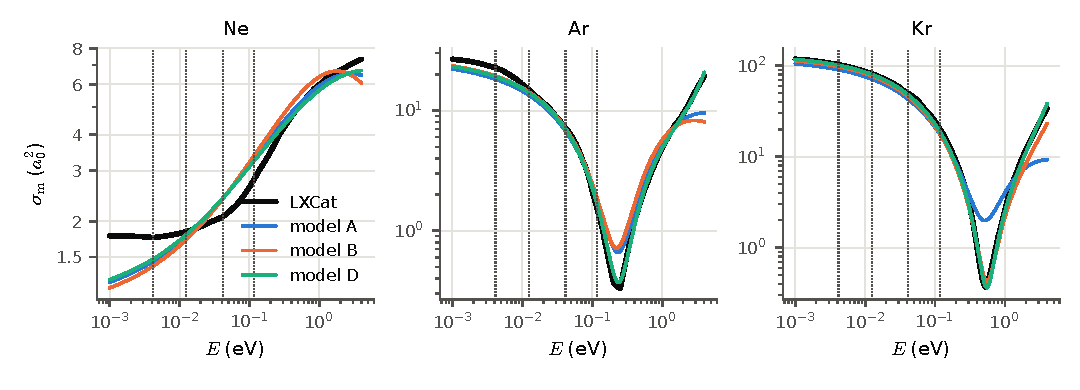
\includegraphics[width=\textwidth]{chapters/ea/fig_sigma.pdf}
\end{center}
\caption{Momentum-transfer cross sections of the LXCat sets used by the
classical kernel and of the three model families. The vertical lines mark the
photon energies of 1, 3, 10 and 28.3~THz.}
\label{ea:fig:sigma}
\end{figure}

\subsection{Numerical method}
\label{ea:sec:numerics}
{\noindent}(1) The radial equation is integrated by the method of Numerov,
on a uniform grid of step $0.01\,a_0$ for the smooth cores and on the
logarithmic grid $r=e^x$, $u=e^{x/2}y$, with
$y''=[(l+\frac12)^2+r^2(2V-k^2)]y$ and step $\Delta x=5\times10^{-4}$, for the
Coulomb-like cores of D. At $r_{\max}=400\,a_0$ the solution is matched to the
Riccati--Bessel functions, which fixes $\delta_l$ and the amplitude, and the
acceleration integrals of Eq.~\eqref{ea:eq:Racc} are accumulated during the
integration and normalized at the end. Partial waves up to $l=12$ are kept.

{\noindent}(2) For the deep models, halving the step, doubling $r_{\max}$ and
raising the largest $l$ to 16 change $G$ by at most $1.4\times10^{-5}$. The
cores of the models A reach $6\times10^{10}$ hartree in krypton, where the
recursion of Numerov is unstable on the uniform grid. The outward growth of the
solution through the forbidden core filters that error out. Starting instead
at a hard wall placed where $h^2\cdot2mV/\hbar^2$ last exceeds 2, with half the
step, changes $G$ of the models A and B by at most $1\times10^{-5}$. The force
identity holds as stated in Sec.~\ref{ea:sec:force}, and detailed balance,
Eq.~\eqref{ea:eq:db}, to $10^{-13}$.

\subsection{The free--free Gaunt factor}
\label{ea:sec:gaunt}
{\noindent}(1) Figure~\ref{ea:fig:G} shows $G=\sigma_+/\sigma_+^{\rm soft}$ for the
deep models. For $\hbar\omega\ll E$ it tends to one, with the slope
$1+\frac12\,\dd\ln\sm/\dd\ln E$ in $\hbar\omega/E$ that Eq.~\eqref{ea:eq:firstorder}
predicts. Below $E\approx\hbar\omega$ it grows as $E^{-3/2}$. There the final
state is near $\hbar\omega$ whatever the initial energy, $\sigma_+$ varies as
$1/k$, and the soft-photon reference vanishes as $k^2$.

\begin{figure}[ht]
\begin{center}
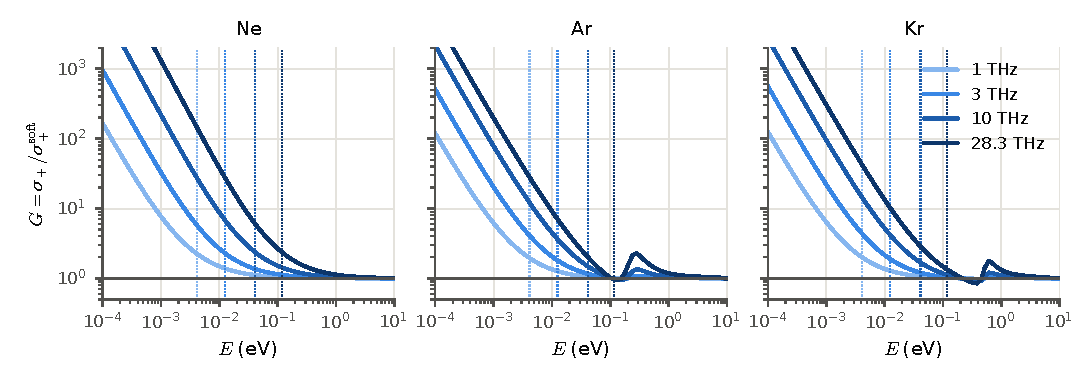
\includegraphics[width=\textwidth]{chapters/ea/fig_G.pdf}
\end{center}
\caption{The free--free Gaunt factor $G=\sigma_+/\sigma_+^{\rm soft}$ of the deep
models at 1, 3, 10 and 28.3~THz. The dotted lines mark $E=\hbar\omega$.}
\label{ea:fig:G}
\end{figure}

{\noindent}(2) A code that needs $\sigma_+$ without solving the scattering
problem can use one of three forms built on $\sm$ alone, the two-energy form of
Eq.~\eqref{ea:eq:twoenergy}, the mean-energy form of Eq.~\eqref{ea:eq:firstorder},
or the mean-momentum form of Eq.~\eqref{ea:eq:meanmom} with the true $\sm$.
Table~\ref{ea:tab:presc} compares them with the exact result of each deep model.
The two-energy form, exact for the zero-range potential, overestimates
$\sigma_+$ of argon by a factor 2.1 for thermal electrons at 28.3~THz. The
polarization tail makes the $p$ wave matter at low energy, since it raises
the $p$-wave phase shift as $\pi\alpha_dk^2/15$ in atomic units rather than as
$k^3$ \cite{ea:OMalleySpruchRosenberg1961}, a law the check script confirms for
the deep models. The mean-energy form falls up to 25\,\% short there.

{\noindent}(3) The mean-momentum form is the best of the three. For neon it
is within 0.5\,\% of the exact result at every energy above $\hbar\omega$ up to
28.3~THz. For argon and krypton it is within 1.2\,\% at 3~THz and 3.3\,\% at
10~THz above $\hbar\omega$. At 28.3~THz it errs by up to 14\,\% in argon and
17\,\% in krypton above $\hbar\omega$, most where the final energy
$E+\hbar\omega$ falls at the Ramsauer minimum of the model, 0.24~eV in argon
and 0.55~eV in krypton. There $\sm$ changes by a large factor across one photon
energy. Table~\ref{ea:tab:presc} shows errors of the same size for thermal
electrons below $\hbar\omega$. In the thermal
averages of Sec.~\ref{ea:sec:thermal} up to 4~THz the form is within 1\,\% of the
exact result for every gas.

\begin{table}[ht]
\caption{The exact Gaunt factor $G$ of the deep models at $E=26$~meV and
0.3~eV, and the two-energy (TE), mean-energy (ME) and mean-momentum (MM) forms
with the model's own $\sm$, as ratios to the exact cross section.}
\label{ea:tab:presc}
\begin{center}
\begin{tabular}{lccccccc}
\toprule
 & & \multicolumn{4}{c}{$E=26$~meV} & \multicolumn{2}{c}{$E=0.3$~eV}\\
gas & $f$ (THz) & $G$ & TE & ME & MM & $G$ & MM\\
\midrule
\tabinput{chapters/ea/tab_presc.tex}
\bottomrule
\end{tabular}
\end{center}
\end{table}

\subsection{Polarization bremsstrahlung}
\label{ea:sec:pbnum}
{\noindent}(1) The term of Eq.~\eqref{ea:eq:pb-op} has the same angular structure
as $\rv$, so in the acceleration form it adds $-m\omega^2\alpha_d/r^2$ to
$V'(r)$. With the cut-off $r^2\to r^2+r_c^2$ of the polarization potential of
model D, Table~\ref{ea:tab:pb} gives the change of $\sigma_+$. It is below 0.7\,\%
up to 3~THz for every gas and energy. At 28.3~THz it reaches $-13$\,\% for slow
electrons in argon, $-8$\,\% in krypton and $+4$\,\% in neon, so a CO$_2$-laser
calculation for a cold gas has to include it. At 1~eV it stays below 1\,\% at
every frequency. Geltman \cite{ea:Geltman1995} studied the same field-induced
dipole in the laser-assisted elastic scattering of Sec.~\ref{ea:sec:strong}.

\begin{table}[ht]
\caption{Change of $\sigma_+$ in percent when the polarization bremsstrahlung
of Eq.~\eqref{ea:eq:pb-op} is added, for the deep models.}
\label{ea:tab:pb}
\begin{center}
\begin{tabular}{lccccc}
\toprule
gas & $E$ (meV) & 1~THz & 3~THz & 10~THz & 28.3~THz\\
\midrule
\tabinput{chapters/ea/tab_pb.tex}
\bottomrule
\end{tabular}
\end{center}
\end{table}

\section{Thermal absorption and the error of the classical kernel}
\label{ea:sec:thermal}

\subsection{The pure gases}
{\noindent}(1) Equation~\eqref{ea:eq:R} gives $\mathcal R(T,\omega)$ from $G$ and
$\sm$ of each model. Table~\ref{ea:tab:R} lists it for the deep models with the
range over the three families. Up to 4~THz the classical kernel is right to
2.5\,\% or better for every gas and temperature, and to 2.8\,\% with any of the
three families. At 10~THz electrons at 300~K
absorb 12\,\% less than the classical kernel says in argon and 7\,\% less in
krypton, and at 28.3~THz 41\,\% and 25\,\% less. In neon the two effects of
Sec.~\ref{ea:sec:soft} cancel to within 3\,\%. Above 0.3~eV the classical kernel
is right to 1.6\,\% at every frequency up to 28.3~THz.

\begin{table}[ht]
\caption{The ratio $\mathcal R=\kappa/\kappa_{\rm cl}$ of Eq.~\eqref{ea:eq:R} for
each gas, from the deep model D, and its range over the models A, B and D.}
\label{ea:tab:R}
\begin{center}
\begin{tabular}{lccccccc}
\toprule
 & & \multicolumn{2}{c}{$T=300$~K} & \multicolumn{2}{c}{$T=0.1$~eV} & \multicolumn{2}{c}{$T=0.63$~eV}\\
gas & $f$ (THz) & D & A--D & D & A--D & D & A--D\\
\midrule
\tabinput{chapters/ea/tab_R.tex}
\bottomrule
\end{tabular}
\end{center}
\end{table}

\subsection{The two fills}
{\noindent}(1) In a mixture each gas contributes to $\kappa_{\rm cl}$ in
proportion to its share $x_g\langle v^3\sm\rangle$, and the ratio of the
mixture is the share-weighted mean of the ratios of its gases. Fluorine
appears only at 0.2 and 0.3\,\%, and its molecular cross section is treated
with the mean-momentum form. At 300~K krypton carries 44\,\% of the classical
absorption of the neon fill and 83\,\% of that of the argon fill, because per
atom its $\langle v^3\sm\rangle$ is 15 times that of neon and 7.6 times that of
argon.

{\noindent}(2) Table~\ref{ea:tab:fills} gives the ratio for both fills, from the
deep models and, in parentheses, from the mean-momentum form with the measured
cross sections alone. Figure~\ref{ea:fig:R} shows it against frequency.

\begin{table}[ht]
\caption{The ratio $\mathcal R=\kappa/\kappa_{\rm cl}$ for the two fills of
Sec.~\ref{ea:sec:why}, from the deep models, and in parentheses from the
mean-momentum form with the LXCat cross sections.}
\label{ea:tab:fills}
\begin{center}
\begin{tabular}{lccccc}
\toprule
fill & $f$ (THz) & $T=300$~K & $T=0.1$~eV & $T=0.63$~eV & $T=1.08$~eV\\
\midrule
\tabinput{chapters/ea/tab_fills.tex}
\bottomrule
\end{tabular}
\end{center}
\end{table}

\begin{figure}[ht]
\begin{center}
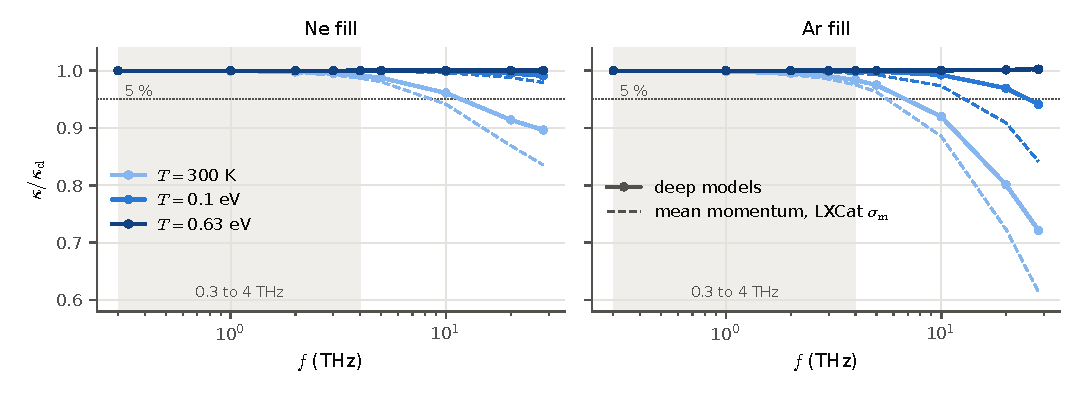
\includegraphics[width=\textwidth]{chapters/ea/fig_R_v2.pdf}
\end{center}
\caption{The ratio of the quantum to the classical absorption coefficient for
the two fills against frequency. Solid lines are the deep models, dashed lines
the mean-momentum form with the LXCat cross sections. The shaded band is the
band of 0.3 to 4~THz proposed for reheating.}
\label{ea:fig:R}
\end{figure}

\subsection{The answer for the laser gas}
{\noindent}(1) In the band of 0.3 to 4~THz proposed for reheating, the
classical kernel differs from the quantum result by
at most 1.6\,\% in either fill at any electron temperature from 300~K to
1.08~eV. The mean-momentum form with the measured cross sections gives at most
2.5\,\%. Both are below the 5\,\% of the criterion of Sec.~\ref{ea:sec:why}, so
the classical kernel holds in that band, and the absorption lengths and
reflectances computed with it stand.

{\noindent}(2) For a CO$_2$ laser on a thermalized fill the classical kernel
fails. At 28.3~THz and 300~K the quantum absorption is 10\,\% below it in the
neon fill and 28\,\% below it in the argon fill, before the polarization
bremsstrahlung of Sec.~\ref{ea:sec:pbnum}. Above 0.3~eV it is right to 1\,\% in
both fills at every frequency studied. A code that heats electrons at such
frequencies should multiply the classical absorption by $\mathcal R$, or
replace the diffusion term of the two-term equation by the jump operator of
Eq.~\eqref{ea:eq:jump} with the mean-momentum cross section.

\section{Electron--ion or electron--atom}
\label{ea:sec:ei}

{\noindent}(1) The ions contribute the effective collision frequency
$\nu_T\Lambda$ \cite{ea:Atzeni2004}, with
\[
\nu_T=\frac{4\sqrt{2\pi}}{3}\,\frac{n_iZ^2e^4}{m^{1/2}(\kB T)^{3/2}},\qquad
\Lambda=\frac{\pi}{\sqrt3}\,\langle g\rangle\,\frac{1-e^{-u}}{u},
\]
the thermal Gaunt factor $\langle g\rangle$ times the factor of stimulated emission
\cite{ea:Kramers1923,ea:KarzasLatter1961}. The atoms
contribute $\kappa$ of Eq.~\eqref{ea:eq:kappa-mb}, which corresponds to the
effective collision frequency $(mN/3\kB T)\langle v^3\sm\rangle\mathcal R$.
With singly charged ions, $n_i=n_e$, the ions win above the electron density at
which the two are equal.

{\noindent}(2) In the Born approximation the thermal Gaunt factor is
$\langle g\rangle=(\sqrt3/\pi)e^{u/2}K_0(u/2)$ \cite{ea:KarzasLatter1961}, valid for
$Ze^2/\hbar v\ll1$. For an electron of energy
$\kB T$, $Ze^2/\hbar v$ is 23 at 300~K and 3.5 at 1.08~eV, and the collisions
are classical. For $x=\omega Ze^2/mv^3\ll1$ and $\hbar\omega\ll\kB T$ the
classical thermal Gaunt factor is that of Scheuer \cite{ea:Scheuer1960},
$\langle g\rangle=(\sqrt3/\pi)\{\ln[(2\kB T)^{3/2}/\pi Ze^2m^{1/2}f]-\frac52\gamma\}$,
with $f$ in hertz. At 300~K and 1~THz, $x$ is about 5 for $v=(\kB T/m)^{1/2}$,
and that formula turns negative. For larger $x$ the classical Gaunt factor
tends to Kramers' value one from above. The estimate used here is the larger
of Scheuer's value and one. At 1~THz, where $u\le0.16$, the Born value exceeds
this estimate at every temperature and bounds the ionic absorption from
above. At 28.3~THz and 300~K, where $u=4.5$, the Born value falls to 0.44,
below Kramers' one, which is then the better estimate.

{\noindent}(3) Table~\ref{ea:tab:ei} and Fig.~\ref{ea:fig:ei} give the density
at which the two kinds of absorption are equal at 1~THz. Ions dominate only in
a cold and dense plasma. At 300~K that takes $7.0\times10^{19}$~m$^{-3}$ in the
neon fill and $1.5\times10^{20}$~m$^{-3}$ in the argon fill with the classical
Gaunt factor, and at 0.63~eV more than $10^{22}$~m$^{-3}$ in both. At 28.3~THz
and 300~K, with Kramers' one, the densities are $2.7\times10^{20}$ and
$4.5\times10^{20}$~m$^{-3}$. The plasma of the laser gas with the beam on,
$2.7\times10^{21}$~m$^{-3}$ at 1.08~eV, absorbs on atoms, and so does the
afterglow while its electrons stay warm. In a thermalized afterglow at
$10^{20}$~m$^{-3}$ and 1~THz the ions absorb 1.4 times as much as the atoms in
the neon fill and 0.7 times as much in the argon fill. The atoms dominate
because $n_e/N$ is small only away from that corner.

\begin{table}[ht]
\caption{Electron density in m$^{-3}$ at which electron--ion and electron--atom
absorption are equal at 1~THz, with the classical estimate of the thermal
Gaunt factor and with the Born value \cite{ea:KarzasLatter1961}. Ions dominate above it.}
\label{ea:tab:ei}
\begin{center}
\begin{tabular}{lccccc}
\toprule
fill & $T$ (eV) & $\langle g\rangle_{\rm cl}$ & $\langle g\rangle_{\rm Born}$ & $n_e$, classical & $n_e$, Born\\
\midrule
\tabinput{chapters/ea/tab_ei.tex}
\bottomrule
\end{tabular}
\end{center}
\end{table}

\begin{figure}[ht]
\begin{center}
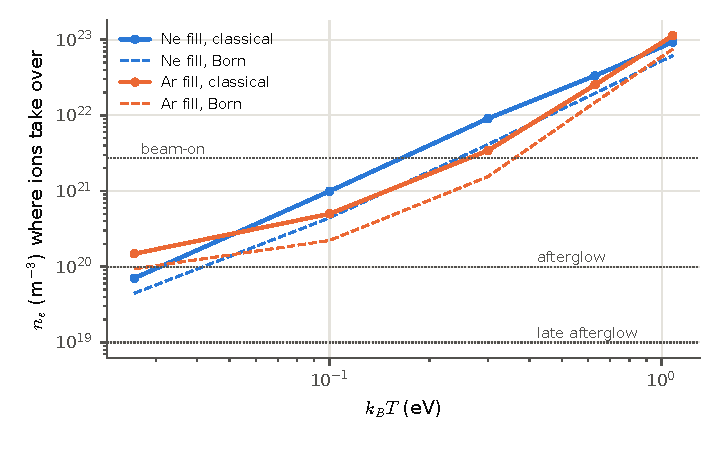
\includegraphics[width=0.75\textwidth]{chapters/ea/fig_ei.pdf}
\end{center}
\caption{The electron density above which electron--ion absorption exceeds
electron--atom absorption at 1~THz. Solid lines use the classical estimate of
the Gaunt factor, dashed lines the Born value. The horizontal lines mark the
electron density of the laser gas with the beam on, $2.7\times10^{21}$~m$^{-3}$,
and in the afterglow, $10^{20}$ and $10^{19}$~m$^{-3}$.}
\label{ea:fig:ei}
\end{figure}

\section{Summary}
\label{ea:sec:summary}

{\noindent}(1) The one-photon free--free cross section of an electron in the
field of an atom is Eq.~\eqref{ea:eq:sigplus}, a sum over partial waves of the
squared dipole integrals, which the acceleration form, Eq.~\eqref{ea:eq:Racc},
makes absolutely convergent. Emission follows from detailed balance,
Eq.~\eqref{ea:eq:db}, and the absorption coefficient of Maxwell electrons carries
the factor $1-e^{-u}$, Eq.~\eqref{ea:eq:kappa-mb}. The kinetic equation is the jump
operator of Eq.~\eqref{ea:eq:jump}, whose Fokker--Planck limit,
Eq.~\eqref{ea:eq:Dfp}, is the field term of the two-term Boltzmann equation at
$\omega\gg\nu$.

{\noindent}(2) The force identity, Eq.~\eqref{ea:eq:force}, reduces the soft-photon
limit to the momentum-transfer cross section, Eq.~\eqref{ea:eq:soft}, and the
classical limit is the Lorentz gas, Eq.~\eqref{ea:eq:kappa-cl}. The cross section
that belongs in the classical formula is therefore $\sm$, which settles the
choice between $\sm$ and the elastic cross section that the literature on
neutral bremsstrahlung leaves open \cite{ea:Buzulutskov2018}.

{\noindent}(3) At finite photon energy the cross section is known exactly for
a zero-range potential, Eq.~\eqref{ea:eq:twoenergy}, which is also the emission
formula of neutral bremsstrahlung, Eq.~\eqref{ea:eq:nbrs}, and in Born
approximation, Eq.~\eqref{ea:eq:meanmom}. Both agree to first order with
Eq.~\eqref{ea:eq:firstorder}, and the model potentials confirm that this order is
universal. Wherever $\hbar\omega\le E$ the mean-momentum form with the true
$\sm$ is accurate to 0.5\,\% for neon at every frequency and to 3.3\,\% for
argon and krypton up to 10~THz, but errs by up to 17\,\% at 28.3~THz near the
Ramsauer minima.

{\noindent}(4) For the laser gas the quantum correction to the classical
kernel is below 1.6\,\% from 0.3 to 4~THz at every temperature, so the
classical kernel holds in that band. It becomes $-10$ to $-28$\,\% at 28.3~THz for electrons at 300~K, where
polarization bremsstrahlung changes the cross section of slow electrons by up
to $-13$\,\%. Electron--ion absorption competes only in a cold afterglow above
about $10^{20}$~m$^{-3}$.

{\noindent}(5) Left open are the exchange of the scattering electron with the
atomic electrons, which a one-body potential only mimics and which the
multichannel R-matrix calculation of Bell and Berrington
\cite{ea:BellBerrington1987} treats for argon, the molecular fluorine, and the
laser-assisted measurements on argon that find photon exchange, up to 12\,\%
of the field-free cross section, where the theory of Kroll and Watson predicts
none \cite{ea:WallbankHolmes1993,ea:WallbankHolmes1994}. The
measured neutral bremsstrahlung \cite{ea:TaylorCaledonia1969,ea:Ranson1977} is the
experimental test of the models at higher photon energies.

\chapterappendix
\section{Partial waves}
\label{ea:app:angular}

{\noindent}(1) Take $\ehat=\hat z$, which the average over the direction of
the electron allows. The matrix elements of $\cos\theta$ are
$\langle l+1,m|\cos\theta|lm\rangle=[((l+1)^2-m^2)/((2l+1)(2l+3))]^{1/2}$ and
vanish for $m'\ne m$. Summing over $m$,
\begin{equation}
\sum_{m=-l}^l\frac{(l+1)^2-m^2}{(2l+1)(2l+3)}
=\frac{(2l+1)(l+1)^2-l(l+1)(2l+1)/3}{(2l+1)(2l+3)}=\frac{l+1}{3},
\end{equation}
and the same steps with $\langle l-1,m|\cos\theta|lm\rangle^2=(l^2-m^2)/((2l-1)(2l+1))$
give $l/3$, which is Eq.~\eqref{ea:eq:angsum}.

{\noindent}(2) The elastic amplitude is
$f(\theta)=k^{-1}\sum_l(2l+1)e^{i\delta_l}\sin\delta_l\,P_l(\cos\theta)$.
In $\int(1-\cos\theta)|f|^2\dd\Omega$ the term with $1$ gives
$(4\pi/k^2)\sum_l(2l+1)\sin^2\delta_l$, and with
$\cos\theta\,P_l=[(l+1)P_{l+1}+lP_{l-1}]/(2l+1)$ the term with $\cos\theta$
gives $(4\pi/k^2)\sum_l2(l+1)\sin\delta_l\sin\delta_{l+1}\cos(\delta_l-\delta_{l+1})$.
Their difference, with
$\sin^2\delta_l+\sin^2\delta_{l+1}-2\sin\delta_l\sin\delta_{l+1}\cos(\delta_l-\delta_{l+1})
=\sin^2(\delta_l-\delta_{l+1})$ and $(2l+1)=(l+1)+l$ regrouped, is
Eq.~\eqref{ea:eq:sigmam}.

\section{The integrals of the zero-range limit}
\label{ea:app:abel}

{\noindent}(1) With $\hat\jmath_1(x)=\sin x/x-\cos x$ and the factor
$e^{-\eta r}$,
\begin{equation}
\int_0^\infty\hat\jmath_1(k'r)\,r\cos(kr)\,e^{-\eta r}\dd r
=\frac1{k'}\int_0^\infty\sin(k'r)\cos(kr)e^{-\eta r}\dd r
-\int_0^\infty r\cos(k'r)\cos(kr)e^{-\eta r}\dd r .
\end{equation}

{\noindent}(2) The first integral is
$\frac1{2k'}\int[\sin(k'+k)r+\sin(k'-k)r]e^{-\eta r}\dd r\to
\frac1{2k'}\big[\frac1{k'+k}+\frac1{k'-k}\big]=\frac{1}{k'^2-k^2}$.

{\noindent}(3) With $\int_0^\infty r\cos(qr)e^{-\eta r}\dd r
=(\eta^2-q^2)/(\eta^2+q^2)^2\to-1/q^2$, the second integral tends to
$-\frac12\big[(k'-k)^{-2}+(k'+k)^{-2}\big]=-(k^2+k'^2)/(k'^2-k^2)^2$.

{\noindent}(4) The difference is
$[(k'^2-k^2)+(k'^2+k^2)]/(k'^2-k^2)^2=2k'^2/(k'^2-k^2)^2$, which is
Eq.~\eqref{ea:eq:abel}. The integral with $\sin kr$ in place of $\cos kr$ tends
to zero for $k\ne k'$, since $\int\sin a r\sin b r\,e^{-\eta r}\dd r$ and
$\int r\sin(qr)e^{-\eta r}\dd r=2\eta q/(\eta^2+q^2)^2$ both vanish with $\eta$.

\section{The numerical checks}
\label{ea:app:checks}

{\noindent}(1) A check script computes every boxed result of these notes and
reproduces every number printed in them, from the tables it writes and from
the prose. It needs numpy, scipy and the LXCat cross sections, runs about
three minutes, and stops with an error if any check fails. The model
potentials are fitted by a second script, and the check script verifies that
the stored parameters reproduce the fit quality and the scattering lengths of
Table~\ref{ea:tab:models}.

{\noindent}(2) It uses four methods. Identities are verified against
independent evaluations, the golden-rule cross section against the plane-wave
Born formula and the Born mean-momentum form to $10^{-14}$. Limits are
verified by their convergence, the zero-range form by narrowing the well and
the soft-photon and Fokker--Planck limits by the order of the remainder. The
numerics are verified by halving the steps and doubling the ranges. The tables
and the numbers in the text are printed from the same computation, and the
script recomputes each number of the prose to the digits shown.

\begin{longtable}{L{4.0cm}cccc}
\caption{The numerical checks of these notes, by the equation, table or section they verify. The second column counts all checks of the row, the third gives the largest deviation among its quantitative checks, relative except for the slopes of Eq.~(\ref*{ea:eq:soft}), which are absolute, the fourth counts the numbers printed in these notes that the script reproduces to their last digit, and the fifth the logical conditions.}\label{ea:tab:checks}\\
\toprule
Equation & Checks & Largest deviation & Printed & Logical\\
\midrule
\endfirsthead
\toprule
Equation & Checks & Largest deviation & Printed & Logical\\
\midrule
\endhead
\bottomrule
\endfoot
Eq.~(\ref*{ea:eq:sigplus}) & 4 & $2.3\times10^{-15}$ &  & \\
Eq.~(\ref*{ea:eq:angsum}) & 8 & $4.4\times10^{-16}$ &  & \\
Eq.~(\ref*{ea:eq:abel}) & 4 & $4.4\times10^{-10}$ &  & \\
Eq.~(\ref*{ea:eq:R01}) & 4 & $1.1\times10^{-2}$ &  & 1\\
Eq.~(\ref*{ea:eq:twoenergy}) & 3 & $4.7\times10^{-16}$ &  & \\
Eq.~(\ref*{ea:eq:nbrs}) & 3 & $1.2\times10^{-16}$ &  & \\
Eq.~(\ref*{ea:eq:db}) & 8 & $8.5\times10^{-14}$ &  & \\
Eq.~(\ref*{ea:eq:kappa-mb}) & 3 & $1.4\times10^{-7}$ &  & \\
Eq.~(\ref*{ea:eq:Dfp}) & 6 & $6.7\times10^{-16}$ &  & \\
Eq.~(\ref*{ea:eq:jump}) & 4 & $6.6\times10^{-5}$ &  & 1\\
Eq.~(\ref*{ea:eq:force}) & 4 & $9.2\times10^{-5}$ &  & \\
Eq.~(\ref*{ea:eq:sigmam}) & 6 & $5.1\times10^{-8}$ &  & \\
Eq.~(\ref*{ea:eq:soft}) & 12 & $5.9\times10^{-3}$ &  & 6\\
Eq.~(\ref*{ea:eq:kappa-cl}) & 4 & $6.9\times10^{-5}$ &  & \\
Eq.~(\ref*{ea:eq:meanmom}) & 4 & $1.6\times10^{-15}$ &  & \\
Eq.~(\ref*{ea:eq:firstorder}) & 6 &  &  & 6\\
Sec.~\ref*{ea:sec:strong} & 9 & $2.0\times10^{-16}$ & 4 & 1\\
Table~\ref*{ea:tab:weak} & 1 &  &  & 1\\
Sec.~\ref*{ea:sec:models} & 50 & $2.6\times10^{-5}$ & 6 & 14\\
Sec.~\ref*{ea:sec:numerics} & 6 & $1.4\times10^{-5}$ & 3 & 1\\
Sec.~\ref*{ea:sec:gaunt} & 20 & $2.2\times10^{-4}$ & 8 & 6\\
Table~\ref*{ea:tab:presc} & 5 &  &  & 5\\
Table~\ref*{ea:tab:pb} & 1 &  &  & 1\\
Sec.~\ref*{ea:sec:thermal} & 22 &  & 15 & 7\\
Sec.~\ref*{ea:sec:ei} & 14 &  & 10 & 4\\
Sec.~\ref*{ea:sec:why} & 11 &  & 11 & \\
Sec.~\ref*{ea:sec:ham} & 5 &  & 5 & \\
Sec.~\ref*{ea:sec:pb} & 1 &  &  & 1\\
Sec.~\ref*{ea:sec:cross} & 1 &  &  & 1\\
Sec.~\ref*{ea:sec:born} & 1 &  &  & 1\\
Sec.~\ref*{ea:sec:force} & 2 &  & 1 & 1\\
Sec.~\ref*{ea:sec:soft} & 2 &  & 2 & \\
Sec.~\ref*{ea:sec:zerorange} & 2 &  & 2 & \\
Sec.~\ref*{ea:sec:firstorder} & 2 &  & 2 & \\
Sec.~\ref*{ea:sec:pbnum} & 4 &  & 3 & 1\\
\midrule
Total & 242 & & 72 & 59\\
\end{longtable}


\raggedright
\begin{thebibliography}{99}
\bibitem{ea:Atzeni2004} S.~Atzeni and J.~Meyer-ter-Vehn, \emph{The Physics of Inertial Fusion}
(Oxford University Press, Oxford, 2004), doi:\href{https://doi.org/10.1093/acprof:oso/9780198562641.001.0001}{10.1093/acprof:oso/9780198562641.001.0001}.
\bibitem{ea:Kramers1923} H.~A.~Kramers, Phil. Mag. \textbf{46}, 836 (1923), doi:\href{https://doi.org/10.1080/14786442308565244}{10.1080/14786442308565244}.
\bibitem{ea:KarzasLatter1961} W.~J.~Karzas and R.~Latter, Astrophys. J. Suppl. \textbf{6}, 167 (1961), doi:\href{https://doi.org/10.1086/190063}{10.1086/190063}.
\bibitem{ea:BunkinFedorov1966} F.~V.~Bunkin and M.~V.~Fedorov, \emph{Bremsstrahlung in a
strong radiation field}, Sov.\ Phys.\ JETP \textbf{22}, 844 (1966), record at
\url{http://www.jetp.ras.ru/cgi-bin/e/index/e/22/4/p844?a=list}.
\bibitem{ea:Margenau1946} H.~Margenau, Phys. Rev. \textbf{69}, 508 (1946), doi:\href{https://doi.org/10.1103/physrev.69.508}{10.1103/physrev.69.508}.
\bibitem{ea:KasyanovStarostin1965} V.~Kas'yanov and A.~Starostin, \emph{On the
theory of bremsstrahlung of slow electrons on atoms}, Sov.\ Phys.\ JETP
\textbf{21}, 193 (1965), record at
\url{http://www.jetp.ras.ru/cgi-bin/e/index/e/21/1/p193?a=list}.
\bibitem{ea:Low1958} F.~E.~Low, Phys. Rev. \textbf{110}, 974 (1958), doi:\href{https://doi.org/10.1103/physrev.110.974}{10.1103/physrev.110.974}.
\bibitem{ea:BurnettKroll1968} T.~H.~Burnett and N.~M.~Kroll, Phys. Rev. Lett. \textbf{20}, 86 (1968), doi:\href{https://doi.org/10.1103/physrevlett.20.86}{10.1103/physrevlett.20.86}.
\bibitem{ea:KrollWatson1973} N.~M.~Kroll and K.~M.~Watson, Phys. Rev. A \textbf{8}, 804 (1973), doi:\href{https://doi.org/10.1103/physreva.8.804}{10.1103/physreva.8.804}.
\bibitem{ea:DalgarnoLane1966} A.~Dalgarno and N.~F.~Lane, ApJ \textbf{145}, 623 (1966), doi:\href{https://doi.org/10.1086/148801}{10.1086/148801}.
\bibitem{ea:OhmuraOhmura1960} T.~Ohmura and H.~Ohmura, ApJ \textbf{131}, 8 (1960), doi:\href{https://doi.org/10.1086/146799}{10.1086/146799}.
\bibitem{ea:Geltman1973} S.~Geltman, J. Quant. Spectrosc. Radiat. Transf. \textbf{13}, 601 (1973), doi:\href{https://doi.org/10.1016/0022-4073(73)90019-8}{10.1016/0022-4073(73)90019-8}.
\bibitem{ea:BellBerrington1987} K.~L.~Bell and K.~A.~Berrington, J. Phys. B: At. Mol. Phys. \textbf{20}, 1329 (1987), doi:\href{https://doi.org/10.1088/0022-3700/20/6/017}{10.1088/0022-3700/20/6/017}.
\bibitem{ea:TaylorCaledonia1969} R.~L.~Taylor and G.~Caledonia, J. Quant. Spectrosc. Radiat. Transf. \textbf{9}, 657 (1969), doi:\href{https://doi.org/10.1016/0022-4073(69)90013-2}{10.1016/0022-4073(69)90013-2}.
\bibitem{ea:Ranson1977} P.~Ranson, O.~Vall\'ee and J.~Chapelle, Rev. Phys. Appl. (Paris) \textbf{12}, 1829 (1977), doi:\href{https://doi.org/10.1051/rphysap:0197700120120182900}{10.1051/rphysap:0197700120120182900}.
\bibitem{ea:Buzulutskov2018} A.~Buzulutskov \emph{et al.}, Astropart. Phys. \textbf{103}, 29 (2018), doi:\href{https://doi.org/10.1016/j.astropartphys.2018.06.005}{10.1016/j.astropartphys.2018.06.005}.
\bibitem{ea:Weingartshofer1977} A.~Weingartshofer \emph{et al.}, Phys. Rev. Lett. \textbf{39}, 269 (1977), doi:\href{https://doi.org/10.1103/physrevlett.39.269}{10.1103/physrevlett.39.269}.
\bibitem{ea:WallbankHolmes1993} B.~Wallbank and J.~K.~Holmes, Phys. Rev. A \textbf{48}, R2515 (1993), doi:\href{https://doi.org/10.1103/physreva.48.r2515}{10.1103/physreva.48.r2515}.
\bibitem{ea:WallbankHolmes1994} B.~Wallbank and J.~K.~Holmes, J. Phys. B: At. Mol. Opt. Phys. \textbf{27}, 5405 (1994), doi:\href{https://doi.org/10.1088/0953-4075/27/21/027}{10.1088/0953-4075/27/21/027}.
\bibitem{ea:Geltman1995} S.~Geltman, Phys. Rev. A \textbf{51}, R34 (1995), doi:\href{https://doi.org/10.1103/physreva.51.r34}{10.1103/physreva.51.r34}.
\bibitem{ea:OMalleySpruchRosenberg1961} T.~F.~O'Malley, L.~Spruch and L.~Rosenberg, J. Math. Phys. \textbf{2}, 491 (1961), doi:\href{https://doi.org/10.1063/1.1703735}{10.1063/1.1703735}.
\bibitem{ea:Schwerdtfeger2019} P.~Schwerdtfeger and J.~K.~Nagle, Mol. Phys. \textbf{117}, 1200 (2019), doi:\href{https://doi.org/10.1080/00268976.2018.1535143}{10.1080/00268976.2018.1535143}.
\bibitem{ea:Kitajima2015} M.~Kitajima \emph{et al.}, J. Phys.: Conf. Ser. \textbf{635}, 012030 (2015), doi:\href{https://doi.org/10.1088/1742-6596/635/1/012030}{10.1088/1742-6596/635/1/012030}.
\bibitem{ea:Kurokawa2011} M.~Kurokawa \emph{et al.}, Phys. Rev. A \textbf{84}, 062717 (2011), doi:\href{https://doi.org/10.1103/physreva.84.062717}{10.1103/physreva.84.062717}.
\bibitem{ea:BuckmanMitroy1989} S.~J.~Buckman and J.~Mitroy, J. Phys. B: At. Mol. Opt. Phys. \textbf{22}, 1365 (1989), doi:\href{https://doi.org/10.1088/0953-4075/22/9/010}{10.1088/0953-4075/22/9/010}.
\bibitem{ea:OMalleyCrompton1980} T.~F.~O'Malley and R.~W.~Crompton, J. Phys. B: At. Mol. Phys. \textbf{13}, 3451 (1980), doi:\href{https://doi.org/10.1088/0022-3700/13/17/023}{10.1088/0022-3700/13/17/023}.
\bibitem{ea:GSZ1969} A.~E.~S.~Green, D.~L.~Sellin and A.~S.~Zachor, Phys. Rev. \textbf{184}, 1 (1969), doi:\href{https://doi.org/10.1103/physrev.184.1}{10.1103/physrev.184.1}.
\bibitem{ea:HagelaarPitchford2005} G.~J.~M.~Hagelaar and L.~C.~Pitchford, Plasma Sources Sci. Technol. \textbf{14}, 722 (2005), doi:\href{https://doi.org/10.1088/0963-0252/14/4/011}{10.1088/0963-0252/14/4/011}.
\bibitem{ea:Scheuer1960} P.~A.~G.~Scheuer, Mon. Not. R. Astron. Soc. \textbf{120}, 231 (1960), doi:\href{https://doi.org/10.1093/mnras/120.3.231}{10.1093/mnras/120.3.231}.
\bibitem{ea:LXCat} L.~C.~Pitchford \emph{et al.}, Plasma Process. Polym. \textbf{14}, 1600098 (2016), doi:\href{https://doi.org/10.1002/ppap.201600098}{10.1002/ppap.201600098}.
\end{thebibliography}
\endgroup


\end{document}
